\documentclass[12pt,fleqn, toc=listof, parskip]{scrreprt}

%%% INCLUDE PACKAGES %%%
%%% Im folgenden Abschnitt können packages eingebunden werden. Packages erweitern Latex um Zusätzliche Befehle und oder passen an wie etwas dargestellt wird. %%%
\usepackage[T1]{fontenc}% Fontkodierung auf das neuere T1 umschalten, behebt umlautfehler beim kopieren aus generierter pdf
\usepackage{lmodern} % needed for scalable fonts
\usepackage[utf8]{inputenc} % Der Latex Code wird in utf8 kodiert. Das ist eine verbreitete Norm die praktisch alle Buchstaben und Sonderzeichen enthält.
\usepackage{microtype}
\usepackage{a4} % Setzt das Format des Dokuments auf DinA4
\usepackage{hyphenat} % Verwaltet Wörter, die nicht richtig getrennt werden und einen Zeilenüberlauf generieren würden.
\usepackage[hyphens]{url} % erlaubt mehr Umbrüche in urls, sehr wichtig für style des Literaturverzeichnisses
\usepackage[ngerman]{babel} % passt bestimmte Ausgaben wie z.B. Datum an die jeweilige Sprache an.
%\usepackage{parskip} % keine automatischer abstand nach paragrafen, use option parskip for KOMA Script classes
%\usepackage{umlaute} % umlaute werden richtig gerendert
\usepackage{adjustbox} % resizing stuff
\usepackage{graphicx} % ermöglicht einbinden von Bildern
\usepackage{setspace} % damit kann man den Zeilenabstand ändern (einfach, eineinhalbfach, doppelt)
%\usepackage{titlesec} % ermöglicht anpassen vom style der chapters, section und subsections
\usepackage{tabularx} % braucht man um Tabellen zu erstellen
\usepackage{wrapfig} % Formatiert Fießtext um Inline Bilder
\usepackage{floatflt} % Ermöglicht Inline Bilder und Tabellen
\usepackage[format=default,font=footnotesize,labelfont=bf]{caption} % Kümmert sich um Darstellung von Bildüberschriften
\usepackage{listings}
\usepackage{color} % Bindet verschiedene Schriftfarben ein.
\usepackage[pdftex,dvipsnames,table,xcdraw]{xcolor}  % Noch mehr Farben.
\usepackage{float} % Man kann für Fließbilder und Tabellen verschiedene Stylings auswählen.

\definecolor{CiteColor}{rgb}{0,0,0.6}
\definecolor{LinkColor}{rgb}{0.6,0,0}
\usepackage[
    bookmarks,
    bookmarksopen=true,
    colorlinks=true,
    linkcolor=LinkColor, 
    citecolor=CiteColor, 
    %linkcolor=black,
    %citecolor=black,
    menucolor=red, 
    anchorcolor=black,
    urlcolor=black,
    filecolor=black,
    backref,
    plainpages=false, 
    pdfpagelabels,
    hypertexnames=false, 
    linktocpage=true
    ]{hyperref}
   % ermöglicht komfortable Referenzierung im Dokument (autoref)
\usepackage[printonlyused]{acronym} % Funktionen und Befehle für Abkürzungsverzeichnis
\usepackage[sort&compress,square,comma,authoryear]{natbib}
\usepackage{bibtopic} % erstellt Literaturverzeichnis
% bibtopic needs a special compilation. use pdflatex -synctex=1 -interaction=nonstopmode %.tex|bibtex %1.aux|bibtex %2.aux|bibtex %3.aux|pdflatex -synctex=1 -interaction=nonstopmode %.tex|pdflatex -synctex=1 -interaction=nonstopmode %.tex in fast translation when in TexMaker
%\usepackage{bpchem}
\usepackage{textcomp}
\usepackage{pdflscape}
\usepackage[colorinlistoftodos,prependcaption]{todonotes}
\usepackage{xargs}   % Use more than one optional parameter in a new commands
\usepackage{amsmath}
\usepackage{multirow}
\usepackage{fancyvrb} % style verbatims
\usepackage{amssymb}
\usepackage{nicefrac} % schöne Brüche im Textfluss
\usepackage{rotating}





%%% INCLUDE COMMANDS %%%
%%% Hier werden neue Commands erstellt. %%%

\newcommand{\bildklein}[3]{  
	\begin{figure}[hp]
	\begin{center}
	\includegraphics[width=0.5\textwidth]{#1}
	\end{center}
	\caption[#2]{#3}
	\end{figure}
}
  	
\newcommand{\bildgross}[3]{  
	\begin{figure}[hp]
	\begin{center}
	\includegraphics[width=0.95\textwidth]{#1}
	\end{center}
	\caption[#2]{#3}
	\end{figure}
}

% binary division in math mode
\makeatletter
\newcommand*{\bdiv}{%
  \nonscript\mskip-\medmuskip\mkern5mu%
  \mathbin{\operator@font div}\penalty900\mkern5mu%
  \nonscript\mskip-\medmuskip
}
\makeatother

% Updated definition, see explanation below
\newcommand*{\fullref}[1]{\hyperref[{#1}]{\autoref*{#1} - \nameref*{#1}}} % One single link

% New commands for todonotes package
\newcommandx{\unsure}[2][1=]{\todo[linecolor=red,backgroundcolor=red!25,bordercolor=red,#1]{#2}}
\newcommandx{\change}[2][1=]{\todo[linecolor=blue,backgroundcolor=blue!25,bordercolor=blue,#1]{#2}}
\newcommandx{\info}[2][1=]{\todo[nolist,linecolor=OliveGreen,backgroundcolor=OliveGreen!25,bordercolor=OliveGreen,#1]{#2}}
\newcommandx{\improvement}[2][1=]{\todo[linecolor=Plum,backgroundcolor=Plum!25,bordercolor=Plum,#1]{#2}}
\newcommandx{\thiswillnotshow}[2][1=]{\todo[disable,#1]{#2}}

\newcommandx{\citepauthor}[2][1=]{[\citeauthor[#1]{#2}]}
\newcommandx{\citetauthor}[2][1=]{\citeauthor[#1]{#2}}

% Labels for items in (nested) itemize (uses bullets/characters)
\renewcommand\labelitemi{\normalfont\bfseries \textendash}% bullet
\renewcommand\labelitemii{\normalfont\bfseries \textendash}% --
\renewcommand\labelitemiii{\normalfont\bfseries \textendash}% *
\renewcommand\labelitemiv{\normalfont\bfseries \textendash}% .

% Put somethin above a sign in math mode
\newcommandx{\aoverb}[2]{\mathrel{\stackrel{\makebox[0pt]{\mbox{\normalfont\tiny \textbf{#1}}}}{#2}}}

% make nested parenthesis grow
%\delimitershortfall=-1pt
\let\Right\right
\let\Left\left
\makeatletter
\def\right#1{\Right#1\@ifnextchar){\!\right}{}}
\def\left#1{\Left#1\@ifnextchar({\!\left}{}}
\makeatother

% my listing style and own language definitions

\renewcommand{\lstlistingname}{Codebeispiel}

\lstset{
  basicstyle=\ttfamily\footnotesize,
  columns=fullflexible,
  keepspaces=true,
  numbers=left,           % where to put the line-numbers
  inputencoding={utf8},
  captionpos=b,   
  literate=%
    {Ö}{{\"O}}1
    {Ä}{{\"A}}1
    {Ü}{{\"U}}1
    {ß}{{\ss}}1
    {ü}{{\"u}}1
    {ä}{{\"a}}1
    {ö}{{\"o}}1
    {~}{{\textasciitilde}}1
}

% Define Language
\lstdefinelanguage{bytetxt}
{
  moredelim=**[is][\color{red}]{@}{@},
  moredelim=**[is][\color{blue}]{!!}{!!},
}

\definecolor{eclipsecgreencomment}{RGB}{63,127,95} % eclipsedoc
\definecolor{eclipsecgreentypes}{RGB}{0,80,50} % eclipsedoc
\definecolor{eclipsecpurplekey}{RGB}{127,0,85} % eclipsedoc
\definecolor{eclipsecblueattrandstr}{RGB}{0,0,192} % eclipsedoc
\definecolor{eclipsecblueemph}{RGB}{206,204,247} % eclipsedoc
\definecolor{eclipsecgrey}{RGB}{128,128,128} % eclipsedoc

\lstdefinestyle{CStyle}{
	language=C,
	morekeywords={__attribute__, msgb_data, msgb_put},
	keywordstyle=\color{eclipsecpurplekey}\bfseries, % keywords
	stringstyle=\color{eclipsecblueattrandstr}, % strings
	commentstyle=\color{eclipsecgreencomment}, % comments
	morecomment=[s][\color{eclipsecblueattrandstr}]{<}{>},
	emph=[0]{%
		uint8_t,uint16_t,uint32_t,
		int8_t,int16_t,int32_t,
		gsmtap_hdr,msgb,
	},
	emph=[1]{%
		version,
		hdr_len,
		type,
		timeslot,
		arfcn,
		signal_dbm,
		snr_db,
		frame_number,
		sub_type,
		antenna_nr,
		sub_slot,
		res,
		PLAIN,
		BURSTMAP_XCCH,
		l2h,l1h,
		STATE_IMSI_CATCHER_SABM,
	},
	emphstyle=[0]{\color{eclipsecgreentypes}}, % own types
	emphstyle=[1]{\color{eclipsecblueattrandstr}}, % attributes
	emphstyle=[2]{\color{eclipsecblueemph}}, % other emphasized keywords like TODO
	breakatwhitespace=false,         
    breaklines=true,                 
    captionpos=b,                    
    keepspaces=true,                 
    numbers=left,                    
    numbersep=5pt,                  
   	numberstyle=\tiny\color{black},
    showspaces=false,                
    showstringspaces=false,
    showtabs=false,                  
    tabsize=4,
}

%%% INITIALISIERUNG
% Hier wird das Dokument initialisiert und bestimmte Formatierungsbefehle ausgeführt. %%%
\defaulthyphenchar=127 % sagt latex das der "Bindestrich" der aktuellen font das Trennzeichen ist. Ermöglicht Anwendung auf kombinierte Wörter wie München-Vorstadt
\hyphenation{Se-bas-ti-an Su-per-ca-li-fra-gi-li-sti-cex-pi-a-li-do-ci-ous Lei-tungs-ver-mitt-lung} % gibt Trennung für bestimmte Wörter vor
%\sloppy % ermöglicht größeren Wortabstand, dadurch weniger Trennung
\pagestyle{empty} % keine kopf oder fussleiste
\bibliographystyle{dinat}
% define citation aliases for Internet links that in most cases lack an author
\defcitealias{bsp:weblinkzitat}{Titel der Beispiel Webseite}
% Textformatierung
\textwidth16cm
\textheight22cm
\topmargin0cm
\oddsidemargin0cm
\evensidemargin0cm
\emergencystretch 3em% % allows latex to strech lines to avoid overfull boxes 

%%% BEGINN
% des Dokuments %%%
\begin{document} 

%%% TITELSEITE 1 und 2 %%%
\begin{center}
	\bigskip \bigskip \bigskip 
	\begin{figure}[ht]
	\centering \includegraphics[width=0.8\linewidth]{figures/hm_logo_svg.pdf}
	\end{figure}
	\vspace*{0.8cm}
	\huge \textbf{Hochschule für angewandte Wissenschaften München} \\
	\bigskip \bigskip \bigskip
	{\huge \textbf{Fakultät für Informatik und Mathematik}} \\
	\bigskip \bigskip \bigskip 
	{\Large \textbf{Masterthesis in Informatik}} \\
	\bigskip \bigskip \bigskip \bigskip \bigskip
	{\Huge \textbf{Ein vom Verschlüsselungsverfahren unabhängiger Man-in-the-Middle Angriff in GSM}} \\  
	\bigskip \bigskip \bigskip
	{\Large Sebastian Stumpf} \\
\end{center}
\vfill
\newpage
\input{misc/emptypage}
\begin{center}
	\bigskip \bigskip \bigskip 
	%\begin{figure}[ht]
	%\centering \includegraphics[width=0.8\linewidth]{figures/hm_logo_svg.pdf}
	%\end{figure}
	\vspace*{0.8cm}
	\huge \textbf{University of Applied Sciences Munich} \\
	\bigskip \bigskip \bigskip
	{\huge \textbf{Department of computer science and mathematics}} \\
	\bigskip \bigskip \bigskip 
	{\Large \textbf{Master thesis in computer science}} \\
	\bigskip \bigskip \bigskip \bigskip \bigskip
	{\Huge \textbf{An encryption independent Man-In-The-Middle Attack in GSM}} \\  
	\bigskip \bigskip \bigskip
	{\Large Sebastian Stumpf} \\
\end{center}
\vfill
\newpage
\input{misc/emptypage}
\bigskip \bigskip \bigskip 
%\begin{figure}[ht]
%\centering \includegraphics[width=0.8\linewidth]{figures/hm_logo_svg.pdf}
%\end{figure}
\vspace*{0.8cm}
\bigskip
\vfill

\begin{tabular}{ll}
{\Large \textbf{Author:}} & {\Large Sebastian Stumpf} \\\\
{\Large \textbf{Matrikelnummer:}} & {\Large 49780514} \\\\
{\Large \textbf{Prüfer:}} & {\Large Prof. Dr. Alf Zugenmaier} \\\\
{\Large \textbf{Semester:}} & {\Large 5. Mastersemester Informatik} \\\\
{\Large \textbf{Abgabedatum:}} & {\Large 06.06.2017}
\end{tabular}

\newpage	
\input{misc/emptypage}

%%% ABSTRACT GERMAN %%%	
%%% ABSTRACT GERMAN %%%	
\section*{Zusammenfassung}
\begin{spacing}{1.2}
\acused{XOR}
In dieser Masterarbeit wird ein neuartiger \ac{MitM} Angriff auf eine Sprachverbindung im \ac{GSM} Netz entwickelt. Der Angriff nutzt den fehlenden Integritätsschutz auf der Funkschnittstelle aus, um in den verschlüsselten Anrufaufbau eines Opfers einzugreifen und den Anruf an ein Mobiltelefon unter Kontrolle des Angreifers umzuleiten. Im theoretischen Teil der Arbeit wird der Angriff entwickelt, seine Machbarkeit mathematisch nachgewiesen und die zugrunde liegende Schwachstelle beschrieben. Im praktischen Teil wird der Angriff für einen \ac{MitM}, in einer Testumgebung mit einer virtualisierten Funkschnittstelle, implementiert und durchgeführt. Die in \ac{GSM} verwendeten Verschlüsselungsverfahren sind Stromchiffren, die die Vertraulichkeit des Datenstroms durch die \ac{XOR}-Kombination mit einem Schlüsselstrom schützen. Es wird gezeigt dass bekannte Teile des Chiffrestroms beliebig manipuliert werden können. Da \ac{GSM} kein Verfahren für den Integritätsschutz spezifiziert, kann der Angreifer die Telefonnummer im ausgehenden Anruf also unbemerkt ersetzen und den Anruf an ein von ihm bestimmtes Endgerät umleiten. Durch die Verknüpfung des eingehenden Anrufs mit einem neuen Anruf bei der ersetzten Nummer, erhält der Angreifer Zugriff auf das geführte Gespräch -- ein \ac{MitM}-Angriff auf die Sprachverbindung. Das Netzwerk und die Endgeräte kümmern sich für den Angreifer um Verschlüsselung und Kodierung der Sprachdaten, da es sich um reguläre \ac{GSM}-Anrufe handelt. Der Angriff ist selbst bei der Verwendung von sicheren Verschlüsselungsverfahren, wie A5/4 anwendbar, da die Verschlüsselung nicht gebrochen werden muss. Auch das aktuelle 3G \ac{AKA} bietet keinen Schutz, da es in \ac{GSM} zwar die gegenseitige Authentifizierung ermöglicht, aber keinen Integritätsschutz unterstützt. Der Angriff erfordert die teilweise Kenntnis der vom Opfer angerufenen Telefonnummer ("`Known Plaintext"'). Diese kann als gegeben angenommen werden, da die Rufnummern in der Regel bekannte Teile aufweisen. \citet{meyer2004man} zeigten, dass es möglich ist, ein \ac{MitM}-Gerät auf der Funkschnittstelle zu installieren, was für die Arbeit vorausgesetzt und nicht näher untersucht wird. Für die praktische Durchführung des Angriffs wird die physikalische Ebene der Funkschnittstelle, auf Basis von Multicast-Sockets, virtualisiert und für diese ein \ac{MitM} implementiert. Die Durchführung des Angriffs erfolgt im Rahmen des Osmocom Projekts. Im letzten Teil der Arbeit wird Bezug zu verwandten Angriffen auf den \ac{GSM}-Standard aufgebaut und die Vorteile gegenüber diese herausgearbeitet.
\end{spacing}
\vfill
\acresetall
%%% ABSTRACT ENGLISH %%%
\section*{Abstract}	% section* heisst die section taucht nicht in der toc auf
\begin{spacing}{1.2}

In this master thesis, a new \ac{MitM} attack on a voice connection in the \ac{GSM} network is being developed. The attack exploits the lack of integrity protection on the radio interface to manipulate a victim's outgoing call and redirect it to a mobile phone designated by the attacker. In the theoretical part of the thesis, the attack and the security flaws it is based on, as well as relations to current attacks are established. In the practical part, the call setup manipulation is verified by a \ac{MitM} on a virtual radio interface. The encryption methods used in \ac{GSM} are stream ciphers. This means the data stream is secured by combining it with a key stream using the exclusive-or (\acs{XOR}) operation. It is shown that a cipher stream generated by a stream cipher can be arbitrarily manipulated if the plaintext is known. Since \ac{GSM} does not specify a procedure for integrity protection, the called phone number in the outgoing call can be replaced by the attacker. The attacker can redirect the call to a mobile entity under control and thus receives the voice traffic from the calling victim. By linking this voice traffic with a new call to the original called number, the attacker creates a \ac{MitM} in between the two communication partners. Because incoming and outgoing calls are valid \ac{GSM} calls, the network and mobile devices take care of the encryption and encoding of the voice data by themselves. This means the attacker has access to the unencrypted communication and can record or manipulate the call as they wish. Since the encryption does not have to be broken, the attack is working even with strong encryption algorithms. Furthermore, the use of the more recent 3G \ac{AKA} instead of the outdated 2G \ac{AKA} provides no protection from the attack. It brings mutual authentication to \ac{GSM} networks, but does not ensure integrity between \ac{MS} and \ac{BTS}. The attack requires partial known plaintext of the called mobile number, which can be assumed in \ac{GSM}. Mobile phone numbers usually have known parts, like the \ac{NDC} or the \ac{CC}. The installation of a \ac{MitM} on the physical level of the real radio frequency interface is not investigated in this work. However, the physical level of the radio interface is virtualized and the \ac{MitM} is inserted into it for the verification of the attack in the practical part. The implementations of the virtual physical interface as well as the \ac{MitM} are carried out within the framework of the Osmocom project.
\end{spacing}
\vfill
\acresetall
\newpage % spring auf die nächste Seite
\vspace*{50px}
An dieser Stelle möchte ich all jenen danken, die durch ihre Unterstützung zu dieser Masterarbeit beigetragen haben.

Harald Welte, für die Einladung zu OsmoCon2017 und OsmoDevCon2017 und die Beantwortung vieler Fragen rund um die Implementierung der virtuellen Um-Schnittstelle. 

Prof. Alf Zugenmaier, für das Teilen der Idee hinter dem Angriff und die regelmäßigen Treffen, in denen er mir mit Rat beiseite stand. 

Meiner Freundin Carmen, für ihr immer offenes Ohr und ihre vielen nützlichen Tipps.

Und nicht zuletzt den Lesern der Arbeit für ihre Zeit und ihr Feedback.

%%% INHALTSVERZEICHNIS %%%
\tableofcontents % Dieser Befehl erstellt den table of contents, das Inhaltsverzeichnis
\newpage

%%% EINSTELLUNGEN 
% für den gesamten Content %%%
\setcounter{tocdepth}{3} % gibt an bis in welche Tiefe Überschriften in der table of contents erscheinen
\setcounter{secnumdepth}{3} % gibt an bis in welche Tiefe Überschriften nummeriert werden
\setlength{\mathindent}{0pt}
\setcounter{page}{1} % Pagecounter beginnt hier bei 1
\pagestyle{headings} % erzeugt eine Kopfzeile aus seitennummer und überschrift des aktuellen Abschnitts
\addtocontents{toc}{\protect\thispagestyle{empty}}

%%% ALLE KAPITEL
% In diesem Abschnitt wirst du deine eigentliche Arbeit schreiben. Jedes Kapitel wird als ein eigenes File angelegt und eingebunden, damit es übersichtlich bleibt. Die chapters liegen im Ordner "chapters". %%%
\begin{spacing}{1.2}
	%%%%%%%%%%%%%%%%%%%%%%%%%%%%%%%%%%%%%%%%%%%%%%%%%%%%%%%%%%%%
%%% Latex Konstrukte
%%%%%%%%%%%%%%%%%%%%%%%%%%%%%%%%%%%%%%%%%%%%%%%%%%%%%%%%%%%
\chapter{Latex Beispiele} \label{hdl:konstrukte}
\section{Aufzählung} \label{hdl:konstrukte_aufzaehlung}
\begin{itemize}
	\item item 1
	\begin{itemize}
		\item sub item 11
		\item sub item 12
		\item sub item 13
	\end{itemize}
	\item item 2
	\item item 3
\end{itemize}
\clearpage

\section{Grafiken} \label{hdl:konstrukte_grafiken}
\begin{figure}[H]
\begin{center}
    \includegraphics[width=1.0\textwidth]{figures/hm_logo_svg.pdf}
	\caption[Kurzeintrag Verzeichnis Beispielbild]{Text unter Beispielbild} \label{fig:beispielbild}
\end{center}
\end{figure}

\begin{wrapfigure}[13]{r}{0.6\textwidth}
  \begin{center}
    \includegraphics[width=0.5\textwidth]{figures/hm_logo_svg.pdf}
  \end{center}
  \caption[Kurzeintrag Verzeichnis Beispielbild wrapped]{Text unter Beispielbild wrapped} \label{fig:beispielbild_wrapped} 
\end{wrapfigure}
Lorem ipsum dolor sit amet, consetetur sadipscing elitr, sed diam nonumy eirmod tempor invidunt ut labore et dolore magna aliquyam erat, sed diam voluptua. At vero eos et accusam et justo duo dolores et ea rebum. Stet clita kasd gubergren, no sea takimata sanctus est Lorem ipsum dolor sit amet. Lorem ipsum dolor sit amet, consetetur sadipscing elitr, sed diam nonumy eirmod tempor invidunt ut labore et dolore magna aliquyam erat, sed diam voluptua. At vero eos et accusam et justo duo dolores et ea rebum. Stet clita kasd gubergren, no sea takimata sanctus est Lorem ipsum dolor sit amet.
Lorem ipsum dolor sit amet, consetetur sadipscing elitr, sed diam nonumy eirmod tempor invidunt ut labore et dolore magna aliquyam erat, sed diam voluptua. At vero eos et accusam et justo duo dolores et ea rebum. Stet clita kasd gubergren, no sea takimata sanctus est Lorem ipsum dolor sit amet. Lorem ipsum dolor sit amet, consetetur sadipscing elitr, sed diam nonumy eirmod tempor invidunt ut labore et dolore magna aliquyam erat, sed diam voluptua. At vero eos et accusam et justo duo dolores et ea rebum. Stet clita kasd gubergren, no sea takimata sanctus est Lorem ipsum dolor sit amet.
\clearpage

\section{Links} \label{hdl:konstrukte_links}
In \ref{hdl:konstrukte} werden Latex Konstrukte vermittelt.\\
In \autoref{hdl:konstrukte_aufzaehlung} werden Latex Aufzählungen vermittelt.
\newline
In \autoref{hdl:konstrukte_links} (Links) werden Latex Links erklärt.
\newline
Ein \fullref{fig:beispielbild_wrapped} (Grafik) kurzer Grafik Link.
\clearpage


\section{Abkürzungen} \label{hdl:konstrukte_abkuerzungen}
Texte, die eine \acs{Abk.} enthalten, die nicht im Duden steht, sollten ein \acl{Abk.}sverzeichnis haben. Eine \ac{Abk.}, die nicht verwendet wird, steht auch nicht im \acl{Abk.}sverzeichnis.
\clearpage

\section{Textgestaltung} \label{hdl:konstrukte_textgestaltung}
\textbf{big}\\
\textit{\glqq italic\grqq}\\
\texttt{monospace}\\
Trenn\-zeichen definieren\\
\clearpage

\section{Zitate} \label{hdl:konstrukte_zitate}
Für das Zitieren von Standards und Weblinks wird das Feld AUTHOR im .bib file missbraucht.\\
\textbf{cite} - nicht benutzen, verhalten nicht klar definiert offenbar\\
\textit{\glqq Dies ist ein Buchzitat mit Seitenzahl.\grqq}\cite[S.92ff.]{bsp:buchzitat}\\
\textit{\glqq Dies ist ein Artikelzitat.\grqq}\cite{bsp:artikelzitat}\\
\textit{\glqq Dies ist ein Weblinkzitat.\grqq}\cite{bsp:weblinkzitat}\\
\textit{\glqq Dies ist Zitat eines Standards mit Jahr.\grqq}\cite{bsp:techspec}\\
\textit{\glqq Dies ist Zitat eines Standards ohne Jahr.\grqq}\citeauthor{bsp:techspec}\\
\textbf{\\citep, natbib functionality}\\
\textit{\glqq Dies ist ein Buchzitat mit Seitenzahl.\grqq}\citep[S.92ff.]{bsp:buchzitat}\\
\textit{\glqq Dies ist ein Artikelzitat.\grqq}\citep{bsp:artikelzitat}\\
\textit{\glqq Dies ist ein Weblinkzitat.\grqq}\citep{bsp:weblinkzitat}\\
\textit{\glqq Dies ist Zitat eines Standards mit Jahr.\grqq}\citep{bsp:techspec}\\
\textit{\glqq Dies ist Zitat eines Standards ohne Jahr.\grqq}\citepauthor{bsp:techspec}\\
\textbf{\\citet, natbib functionality}\\
Dies ist ein inline Buchzitat mit Seitenzahl wie in \citet[S.92ff.]{bsp:buchzitat}.\\
Dies ist ein inline Artikelzitat wie in \citet{bsp:artikelzitat}.\\
Dies ist ein inline Weblinkzitat wie in \citet{bsp:weblinkzitat}.\\
Dies ist ein inline Zitat eines Standards mit Jahr wie in \citet{bsp:techspec}.\\
Dies ist ein inline Zitat eines Standards ohne Jahr wie in \citetauthor{bsp:techspec}.\\
\textbf{\\citetalias and citepalias, natbib functionality}\\
After defining an alias by the \textbackslash defcitealias\{bsp:buchzitat\}\{buchzitat-alias\} this can be used in text and after a paragraph.\\
\defcitealias{bsp:buchzitat}{buchzitat-alias}
\textit{\glqq Dies ist ein Webseitenzitat.\grqq}\citepalias[S.92ff.]{bsp:buchzitat}\\
Dies ist ein inline Webseitenzitat wie in \citetalias[S.92ff.]{bsp:buchzitat}.\\
\clearpage

\section{Tabellen} \label{hdl:konstrukte_tabellen}
\begin{table}[h]\footnotesize
\begin{center}
\begin{tabular}{ | p{3cm} | p{5cm} | p{5cm} |}
  \hline
    \textbf{Überschrift 1} & \textbf{Überschrift 2} & \textbf{Überschrift 3} \\
  \hline
    Inhalt 11 & Inhalt 12 & Inhalt 13 \\
  \hline
    Inhalt 21 & Inhalt 22 & Inhalt 23 \\
  \hline
    Inhalt 31 & Inhalt 32 & Inhalt 33 \\
  \hline
\end{tabular}
\caption[Kurzeintrag Verzeichnis Beispiel Tabelle]{Text unter Beispiel Tabelle} \label{tab:Beispieltabelle}
\end{center}
\end{table}
\clearpage

%%%%%%%%%%%%%%%%%%%%%%%%%%%%%%%%%%%%%%%%%%%%%%%%%%%%%%%%%%%
%%% Latex Konstrukte ENDE
%%%%%%%%%%%%%%%%%%%%%%%%%%%%%%%%%%%%%%%%%%%%%%%%%%%%%%%%%%%
	%%%%%%%%%%%%%%%%%%%%%%%%%%%%%%%%%%%%%%%%%%%%%%%%%%%%%%%%%%%
%%% Einleitung
%%%%%%%%%%%%%%%%%%%%%%%%%%%%%%%%%%%%%%%%%%%%%%%%%%%%%%%%%%%
\chapter{Einleitung} \label{hdl:einleitung}

Seit der Einführung von \ac{GSM} 1992 hat sich der Mobilfunk stetig weiterentwickelt. So wurden neue, schnellere und sicherere Standards für Mobilfunknetzwerke spezifiziert und ausgerollt. Weil das \ac{GSM}-Netz aber wegen seiner bestehenden und weit verbreiteten Infrastruktur flächendeckenden Empfang liefert und kostengünstig ist, wird es in den meisten Regionen trotz Ausbau der 3G und 4G Netze weiterhin unterstützt und verwendet \citep{opensignal}. In Japan, Korea und Singapur ist die Abschaltung des 2G Netzes bereits erfolgt und in Australien bis September 2017 geplant. Das Ziel dabei ist vor allem die Wiederverwendung der begehrten, aber von \ac{GSM} belegten Frequenzen im 900 MHz Band. In Europa wird laut \citet{heise:newsticker-3582914} aktuell die Unterstützung und Instandhaltung der Infrastruktur von \ac{GSM} bis etwa 2020 vorausgesagt - viele Netzanbieter halten sich diesbezüglich bedeckt. Da vor allem im \ac{IoT} Bereich und für die \ac{M2M} Kommunikation viele \ac{GSM}-Module verwendet werden, die die neueren Standards nicht unterstützen, hält man sich in einigen Ländern wie Deutschland mit konkreten Angaben ganz zurück. Der Lebenszyklus dieser meist im Embedded-Bereich verwendeten Geräte ist in der Regel hoch und ohne \ac{GSM} müssten sie ersetzt werden, was hohe Kosten verursachen würde. Auch 2017 wird noch in den Ausbau von \ac{GSM}-Netzwerken investiert. In Mexiko wird zum Beispiel für schwer erreichbare Regionen von Non-Profit-Organisationen der \ac{GSM} Netzausbau auf Basis von Open-Source-Software des Osmocom Projektes vorangetrieben \citep{osmocom:news-rhizomatica}. Es wird derzeit angenommen, dass das 3G Netz als Übergangstechnologie vom sprachbasierten \ac{GSM} zum datenbasierten \ac{LTE} früher abgeschaltet wird als \ac{GSM}. Die \ac{GSM}-Infrastruktur wird, wenn man von der derzeitigen Entwicklung ausgeht, also noch lange erhalten bleiben. Die folgenden Zitate stützen diese Behauptung.

\textit{"`In terms of global reach, cellular networks already cover 90 percent of the world’s population.
WCDMA and LTE are catching up, but GSM will offer superior coverage in many markets for
years to come."'} \citep{Ericsson:2016:Uen:284-23-3278}

\textit{"`Speziell für M2M Anwendungen könnte GSM über 2020 hinaus weiterhin relevant bleiben."'} \citep[Tom Tesch]{heise:newsticker-3582914}

\textit{"`We are still maintaining our old networks, and modernising the network, also still delivering 2G and 3G services to the customer. And yes, 2G will continue longer than we expected"'} \citep[Matthias Sauder, Vodafone]{mobileworldlive:long-life-2g}

Der wohl noch länger andauernden Laufzeit von \ac{GSM} stehen dessen veraltete Sicherheitsmechanismen und die Einstellung von Mobilfunkanbietern und Herstellen, diese zu überarbeiten gegenüber. Harald Welte fasst diese in seinem Blog zum Thema Sicherheit zusammen.

\textit{"`GSM equipment manufacturers and mobile operators have shown no interest in fixing gaping holes in their security system."'} \citep[Harald Welte]{laforge:blog-20101112}

So wird \ac{GSM} ohne größere Veränderungen auf dem gleichen Stand der Technik wie vor 30 Jahren betrieben. Trotz einiger Versuche die Sicherheit zu verbessern, wie die Einführung der gegenseitigen Authentifizierung oder die Spezifikation von neuen Verschlüsselungsalgorithmen wie A5/4, bleibt \ac{GSM} verwundbar und anfällig für eine Vielzahl von Angriffen. Gründe dafür sind Schwachstellen in den Anpassungen der Sicherheitsmechanismen und die verzögerte Einführung dieser von den Netzanbietern. Das auch für \ac{GSM} spezifizierte \ac{UMTS}-\ac{AKA} gewährleistet in \ac{GSM} zum Beispiel gegenseitige Authentifizierung, aber keinen Integritätsschutz, eine Schwachstelle in der Spezifikation. Der in dieser Arbeit vorgestellte \ac{MitM}-Angriff nutzt diese Schwachstelle, sowie in \ac{GSM} unverschlüsselt preisgegebene Informationen, um in den Anrufaufbau einzugreifen und ein Telefonat zu einem Angreifer umzuleiten. Der Eingriff liegt in der Manipulation der angerufenen Telefonnummer in der verschlüsselten, für den Anrufaufbau zuständigen Signalisierungsnachricht. Der Angriff verdeutlicht die Notwendigkeit, Möglichkeiten für den Schutz der Integrität für den \ac{GSM}-Standard zu spezifizieren und in den \ac{GSM}-Netzwerken einzuführen. Verschlüsselung ohne Integritätsschutz stellt eine gravierende Schwachstelle dar. Vor allem im Hinblick auf die voraussichtlich noch lange Laufzeit von \ac{GSM}, muss diese dringend behoben werden.
	%%%%%%%%%%%%%%%%%%%%%%%%%%%%%%%%%%%%%%%%%%%%%%%%%%%%%%%%%%%
%%% Ziel
%%%%%%%%%%%%%%%%%%%%%%%%%%%%%%%%%%%%%%%%%%%%%%%%%%%%%%%%%%%
\chapter{Ziel} \label{hdl:ziel}
Ziel dieser Arbeit ist es, einen \ac{MitM}-Angriff auf eine verschlüsselte Sprachverbindung im \ac{GSM}-Netz umzusetzen. Der Angriff soll den fehlenden Integritätsschutz der Kommunikation zwischen Netzteilnehmer und Netzwerk ausnutzen, um ein ausgehendes Telefonat an eine vom Angreifer bestimmte Telefonnummer umzuleiten. Die Verschlüsselung soll nicht gebrochen werden, der kryptografische Schlüssel wird also als unbekannt vorausgesetzt.

Der Angriff soll sowohl theoretisch entwickelt, als auch praktisch umgesetzt werden. Im theoretischen Teil soll die Möglichkeit der Identifizierung der für den Anrufaufbau zuständigen Nachricht im Nachrichtenfluss gezeigt und die Machbarkeit der Manipulation dieser Nachricht, ohne Kenntnis des kryptografischen Schlüssels, mathematisch nachgewiesen werden. Im praktischen Teil der Arbeit soll der Angriff innerhalb einer Testumgebung, anhand eines vom Opfer ausgehenden Anrufs, praktisch durchgeführt werden. Die Implementierung des Angriffs und dafür nötiger Anwendungen soll das Open-Source-Projekt Osmocom nutzen. Für den Aufbau der Testumgebung sollen die Projekte osmoBTS (die \ac{BTS}) und osmocomBB (die \ac{MS}) über eine virtuelle Funkschnittstelle verbunden werden. Die virtuelle Funkschnittstelle soll die Übertragung der Nachrichten über \ac{UDP}/\ac{IP}, statt einem Funksignal ermöglichen. Für die virtuelle Funkschnittstelle soll eine \ac{MitM}-Anwendung implementiert werden, die Zugriff auf die Kommunikation zwischen \ac{MS} und \ac{BTS} hat. Der ausgehende Anruf des Opfers soll vom \ac{MitM} an eine vom Angreifer bestimmte Rufnummer umgeleitet werden. Die Weiterleitung der Audiodaten, vom Mobilfunktelefon des Angreifers an die ersetzte Rufnummer, ist nicht Teil dieser Arbeit, ebenso wie die Umsetzung des \acp{MitM}-Angriffs auf der realen Funkschnittstelle.

Das übergreifende Ziel ist es, den Bedarf an Integritätsschutz generell und speziell in \ac{GSM} zu verdeutlichen. Es soll gezeigt werden, dass die fehlende Integrität die Verschlüsselung nutzlos macht, wenn ein Angreifer Teile der verschlüsselten Signalisierungsnachrichten kennt. 
	\input{misc/emptypage}
	\chapter{Grundlagen} \label{hdl:einfuehrung-gsm}

Folgenden Abschnitte umfassen Grundlagen, die für das Verständnis der weiteren Kapitel der Arbeit von Nutzen sind. Es wird auf die \ac{GSM}-Netzarchitektur, verschiedene von \ac{3GPP} spezifizierte Protokolle und Sicherheitsmechanismen in \ac{GSM} eingegangen.

\section{GSM Architektur} \label{hdl:einfuehrung-gsm_architektur}

\acused{A3}
\acused{A8}

Die \ac{GSM}-Netzarchitektur ist, wie in \autoref{fig:gsm-architecture} zu sehen, hierarchisch aufgebaut. Auf \ac{GPRS} Komponenten sowie Schnittstellen der Infrastruktur zu 3G und 4G Netzen wird nicht eingegangen. Ein \ac{BSS} ist zuständig für Verwaltung und den Betrieb der Funkschnittstelle die den verbundenen Endgeräten die Übertragung von Sprache und Daten ermöglicht. Die Funktion des \ac{NSS} eines Netzbetreibers besteht in der Vermittlung von Gesprächs- oder Datenverbindungen innerhalb des eigenen \ac{BSS}, oder zu Partnernetzwerken wie dem Festnetz und Mobilfunknetzen anderer Anbieter. Hier wegen mangelnder Relevanz nicht erklärte Begriffe und Komponenten finden sich im Anhang in \autoref{hdl:a_gsm_arch}.

\begin{figure}[H]
	\centering 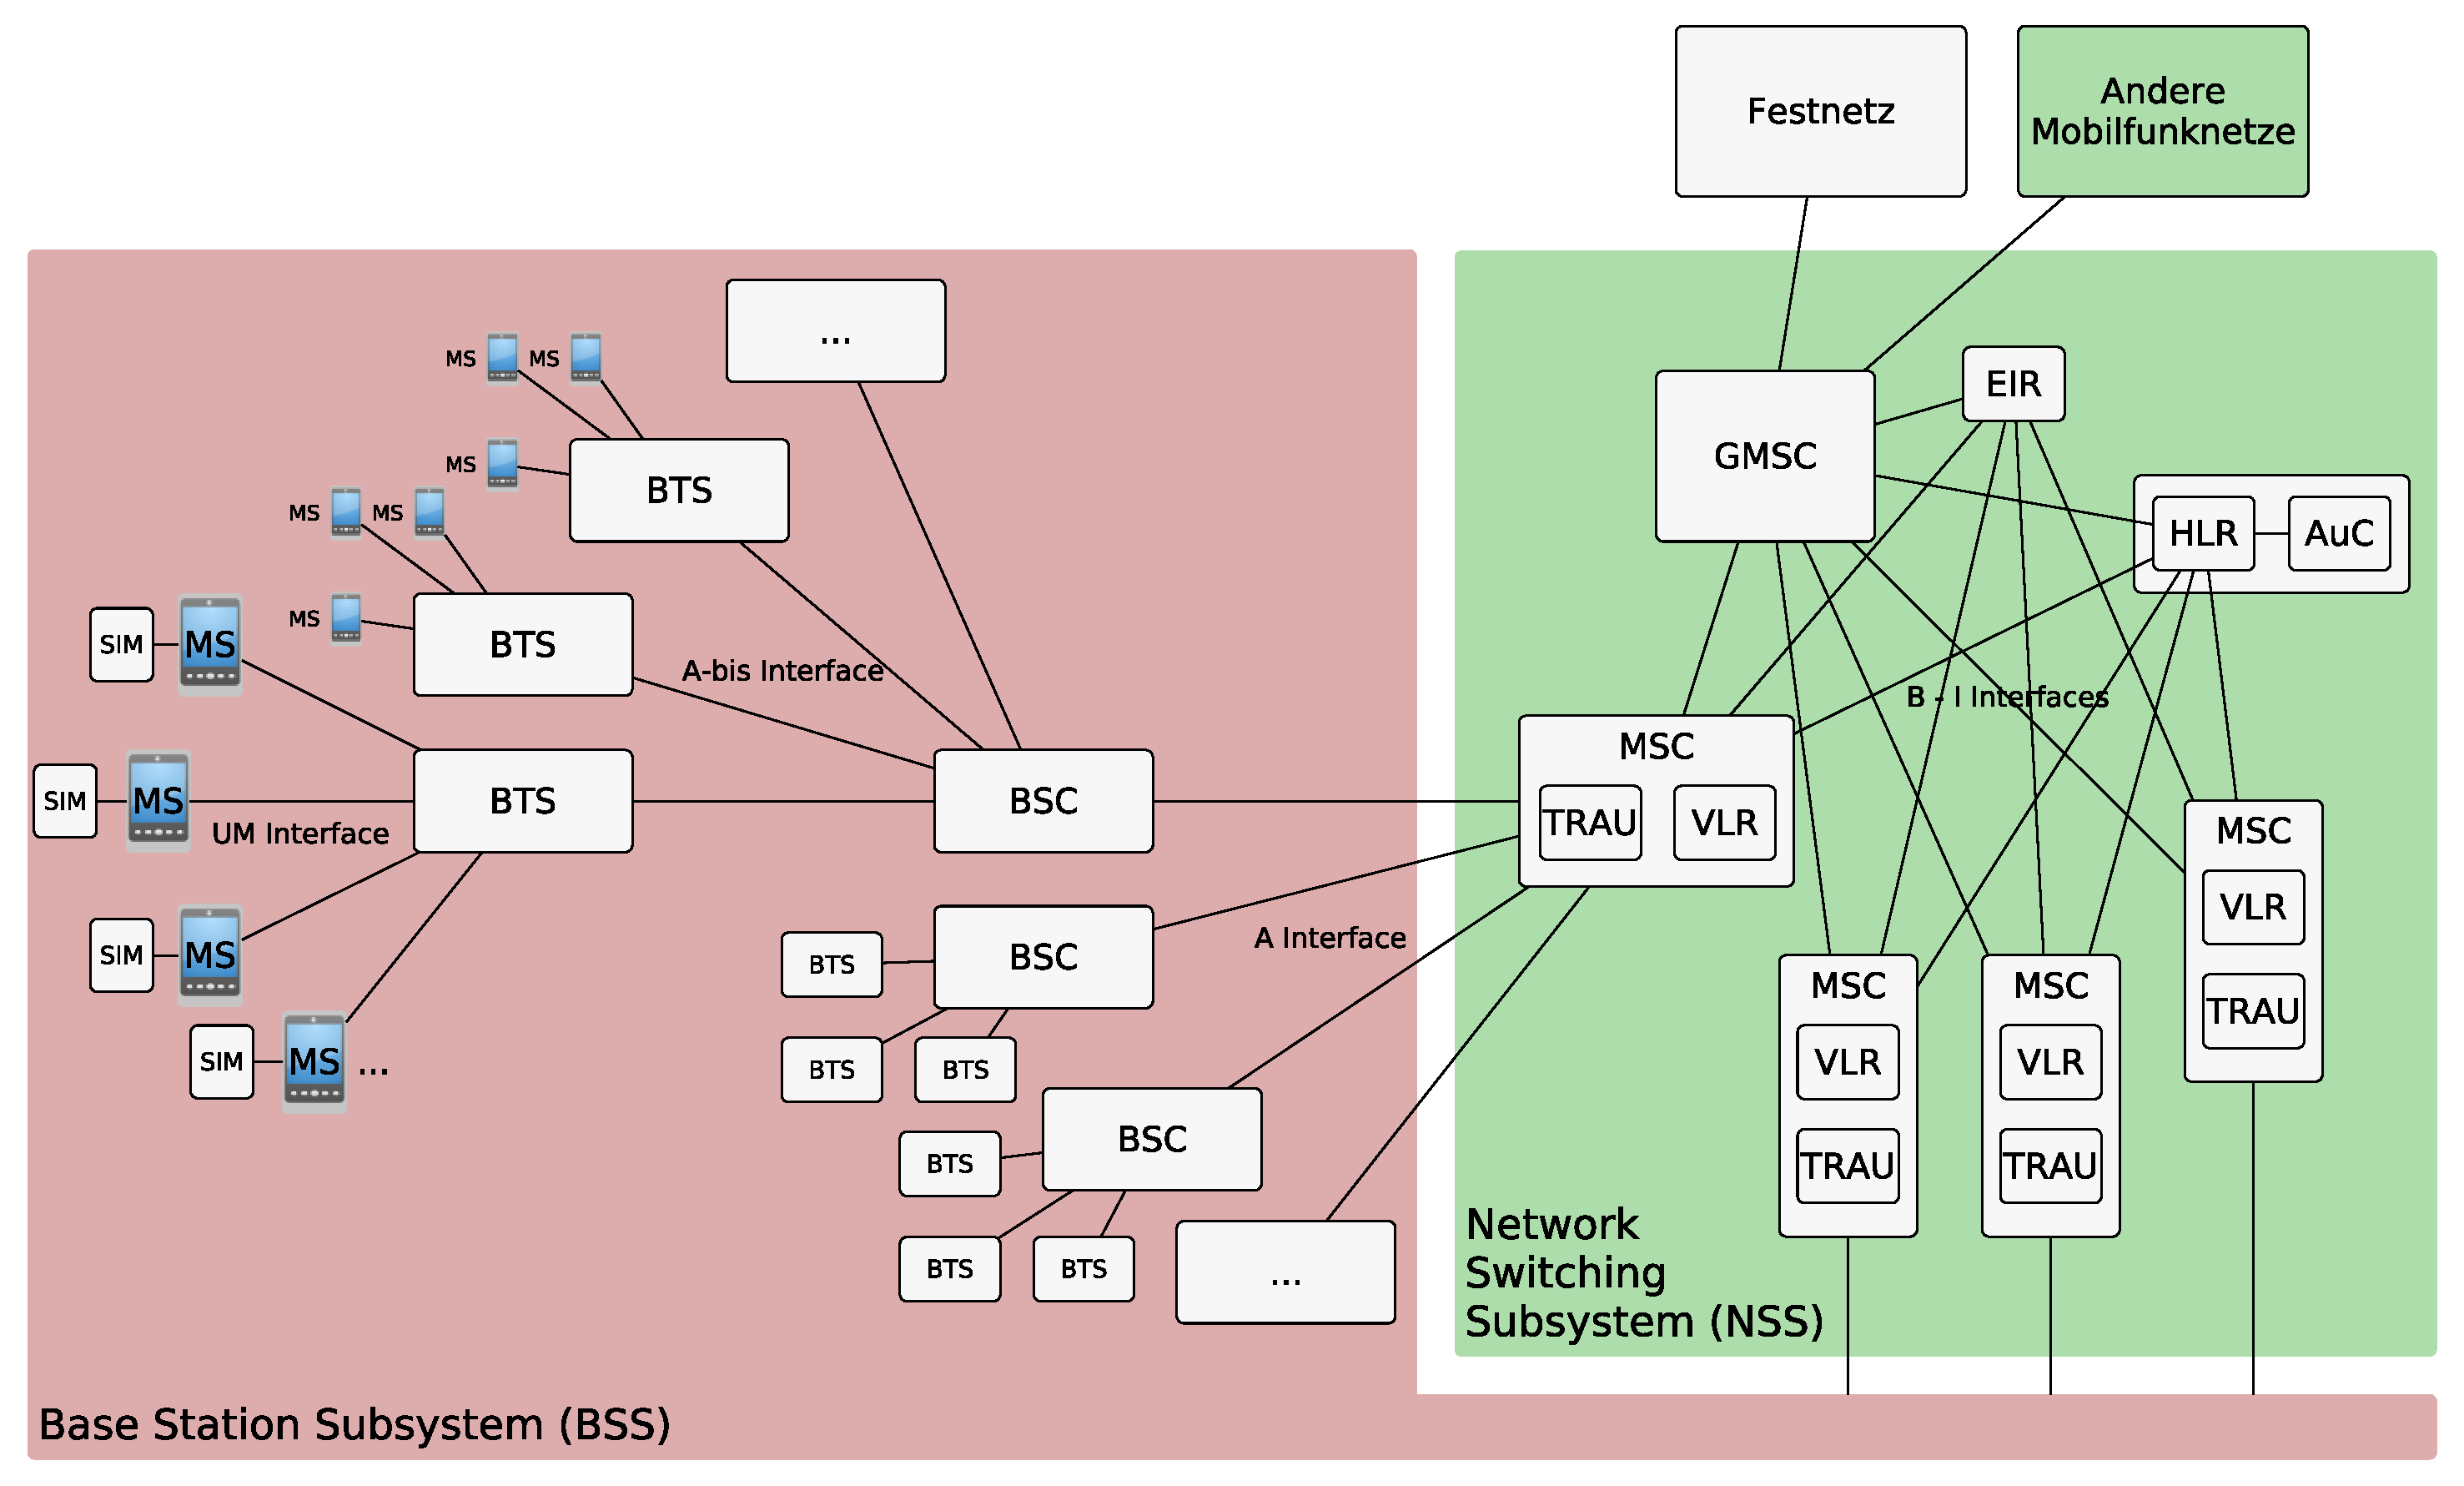
\includegraphics[width=1.0\linewidth]{figures/gsm_network_architecture.pdf}
	  \caption[Die GSM Netzarchitektur]{Die \ac{GSM}-Netzarchitektur, erstellt mit yEd nach \citep{schnabel2003kommunikationstechnik}} \label{fig:gsm-architecture} 
\end{figure}

\begin{description}
\item[\acused{MS}\acs{MS} - \acl{MS}] Die \ac{MS} bezeichnet das mobile Endgerät, das Zugriff auf das Netzwerk erhält. Um die volle Funktionalität des Netzwerks nutzen zu können braucht man eine \acs{SIM}-Karte. Auf ihr sind \ac{IMSI} und geheimer Schlüssel eines Netzteilnehmers gespeichert. Die vom Anbieter zugeteilte \ac{IMSI} identifiziert den Nutzer eindeutig, womit ihm die verwendeten Dienste in Rechnung gestellt werden können. Das \ac{SIM} Modul ist ein Mikrocontroller, der zusammen mit dem \ac{AuC} Zugriff auf den geheimen Schlüssel \acs{Ki} und die Algorithmen \acs{A3} (Authentifizierung) und \acs{A8} (Schlüsselgenerierung) hat. Neben \ac{IMSI} und \acs{Ki} können auch Benutzerdaten wie persönliche Kontakte und der Anrufverlauf gespeichert werden.
\item[\acused{BTS}\acs{BTS} - \acl{BTS}] Die \ac{BTS} kommuniziert über die Funkschnittstelle auf einer oder mehreren zugewiesenen Trägerfrequenzen mit den \acp{MS}. Dabei werden Uplink- und Downlinkfrequenz von einer \ac{ARFCN} definiert. Damit sich benachbarte \ac{BTS} nicht gegenseitig stören, werden ihnen sich nicht überlappende Trägerfrequenzen zugeteilt. Mehrere \acp{MS} können gleichzeitig mit einer \ac{BTS} verbunden sein. 
\item[\acused{BSC}\acs{BSC} - \acl{BSC}] Der \ac{BSC} kann über das Abis Interface auf dem \ac{OML} mehrere \acp{BTS} verwalten und vermittelt Daten vom \ac{NSS} an den zuständigen \ac{BTS}. Nutzdaten von von Mobiltelefonen werden an das \ac{NSS} weitergeleitet.
\item[\acused{MSC}\acs{MSC} - \acl{MSC}] Mehrere \acp{BSC} sind über ein \ac{MSC} mit dem Kernnetzwerk und anderen Netzwerken verbunden. Das \ac{MSC} ist Teil des \ac{SS7} Netzwerks, hat also Zugriff auf alle Komponenten darin. Das \ac{VLR} ist meist direkt im \ac{MSC} integriert.
\item[\acused{HLR}\acs{HLR} - \acl{HLR}] Das \ac{HLR} enthält eine Datenbank mit Informationen aller Netzteilnehmer des Providers sowie das \ac{AuC} mit den Algorithmen \ac{A3} und \ac{A8}. Gespeichert sind Vertragsdetails, Zugriffsberechtigungen auf Netzdienste, aktuelles Guthaben, \acs{Ki}, \ac{MSRN}, aktuelles \ac{VLR} und \ac{MSISDN} zu jeder \ac{IMSI}. Die \ac{MSRN} ermöglicht das Auffinden des Teilnehmers in fremden Netzen beim Roaming. Das aktuelle \ac{VLR} wird für die Lokalisierung im eigenen Netz verwendet. Falls sich beim \ac{LAU} eine \ac{MS} aus dem Zuständigkeitsbereich des \ac{MSC} entfernt, muss im \ac{HLR} die Adresse des \ac{VLR} angepasst werden.
\item[\acused{VLR}\acs{VLR} - \acl{VLR}] Der zeitaufwendige Zugriff des \ac{MSC} auf das \ac{HLR} über das \ac{SS7} wird durch das \ac{VLR} umgangen. Es enthält eine Kopie der Daten des \ac{HLR} und zusätzlich die Felder \ac{TMSI} und \ac{LAI}. Mit dem \ac{LAI} kann der \ac{BSC}, in dessen Zuständigkeitsbereich sich der Teilnehmer gerade befindet, identifiziert werden. Die Teilnehmerdaten sind über \ac{TMSI}, \ac{IMSI} und die \ac{MSRN} indiziert. Die Adresse des \ac{HLR} wird benötigt um Authentifizierungsanfragen an dieses weiterzuleiten.
\item[\acs{Um}-Schnittstelle] (siehe \autoref{hdl:einfuehrung-gsm_schnittstellen_protokolle-um_interface})
Die Funk- oder Radioschnittstelle wird für den Datentransfer zwischen \ac{MS} und \ac{BTS} verwendet. \ac{FDMA} ermöglicht die Kommunikation mit verschiedenen \ac{BTS} und legt die Richtung des Datenflusses (Uplink / Downlink) fest. Mit \ac{TDMA} werden verschiedene Kommunikationskanäle mit einer \ac{BTS} definiert, durch die verschiedene Typen von Signalisierungsinformationen und Daten unterschieden werden können. Übertragene Nachrichten sind kodiert und in der Regel verschlüsselt.
\end{description}

\section{GSM Signalisierungsprotokolle} \label{hdl:einfuehrung-gsm_schnittstellen_protokolle}

Logische Kanäle (siehe \autoref{tab:logical-channels}) können entweder Signalisierungsinformationen oder Nutzdaten übertragen. Wegen der unterschiedlichen Anforderungen werden in \ac{GSM} dafür zwei Protokollstapel definiert - Signaling Plane und User Plane \cite[Kap. 5.2, 5.3]{eberspacher:2008:gsm-architecture}.

\begin{figure}[H]
  \begin{center}
    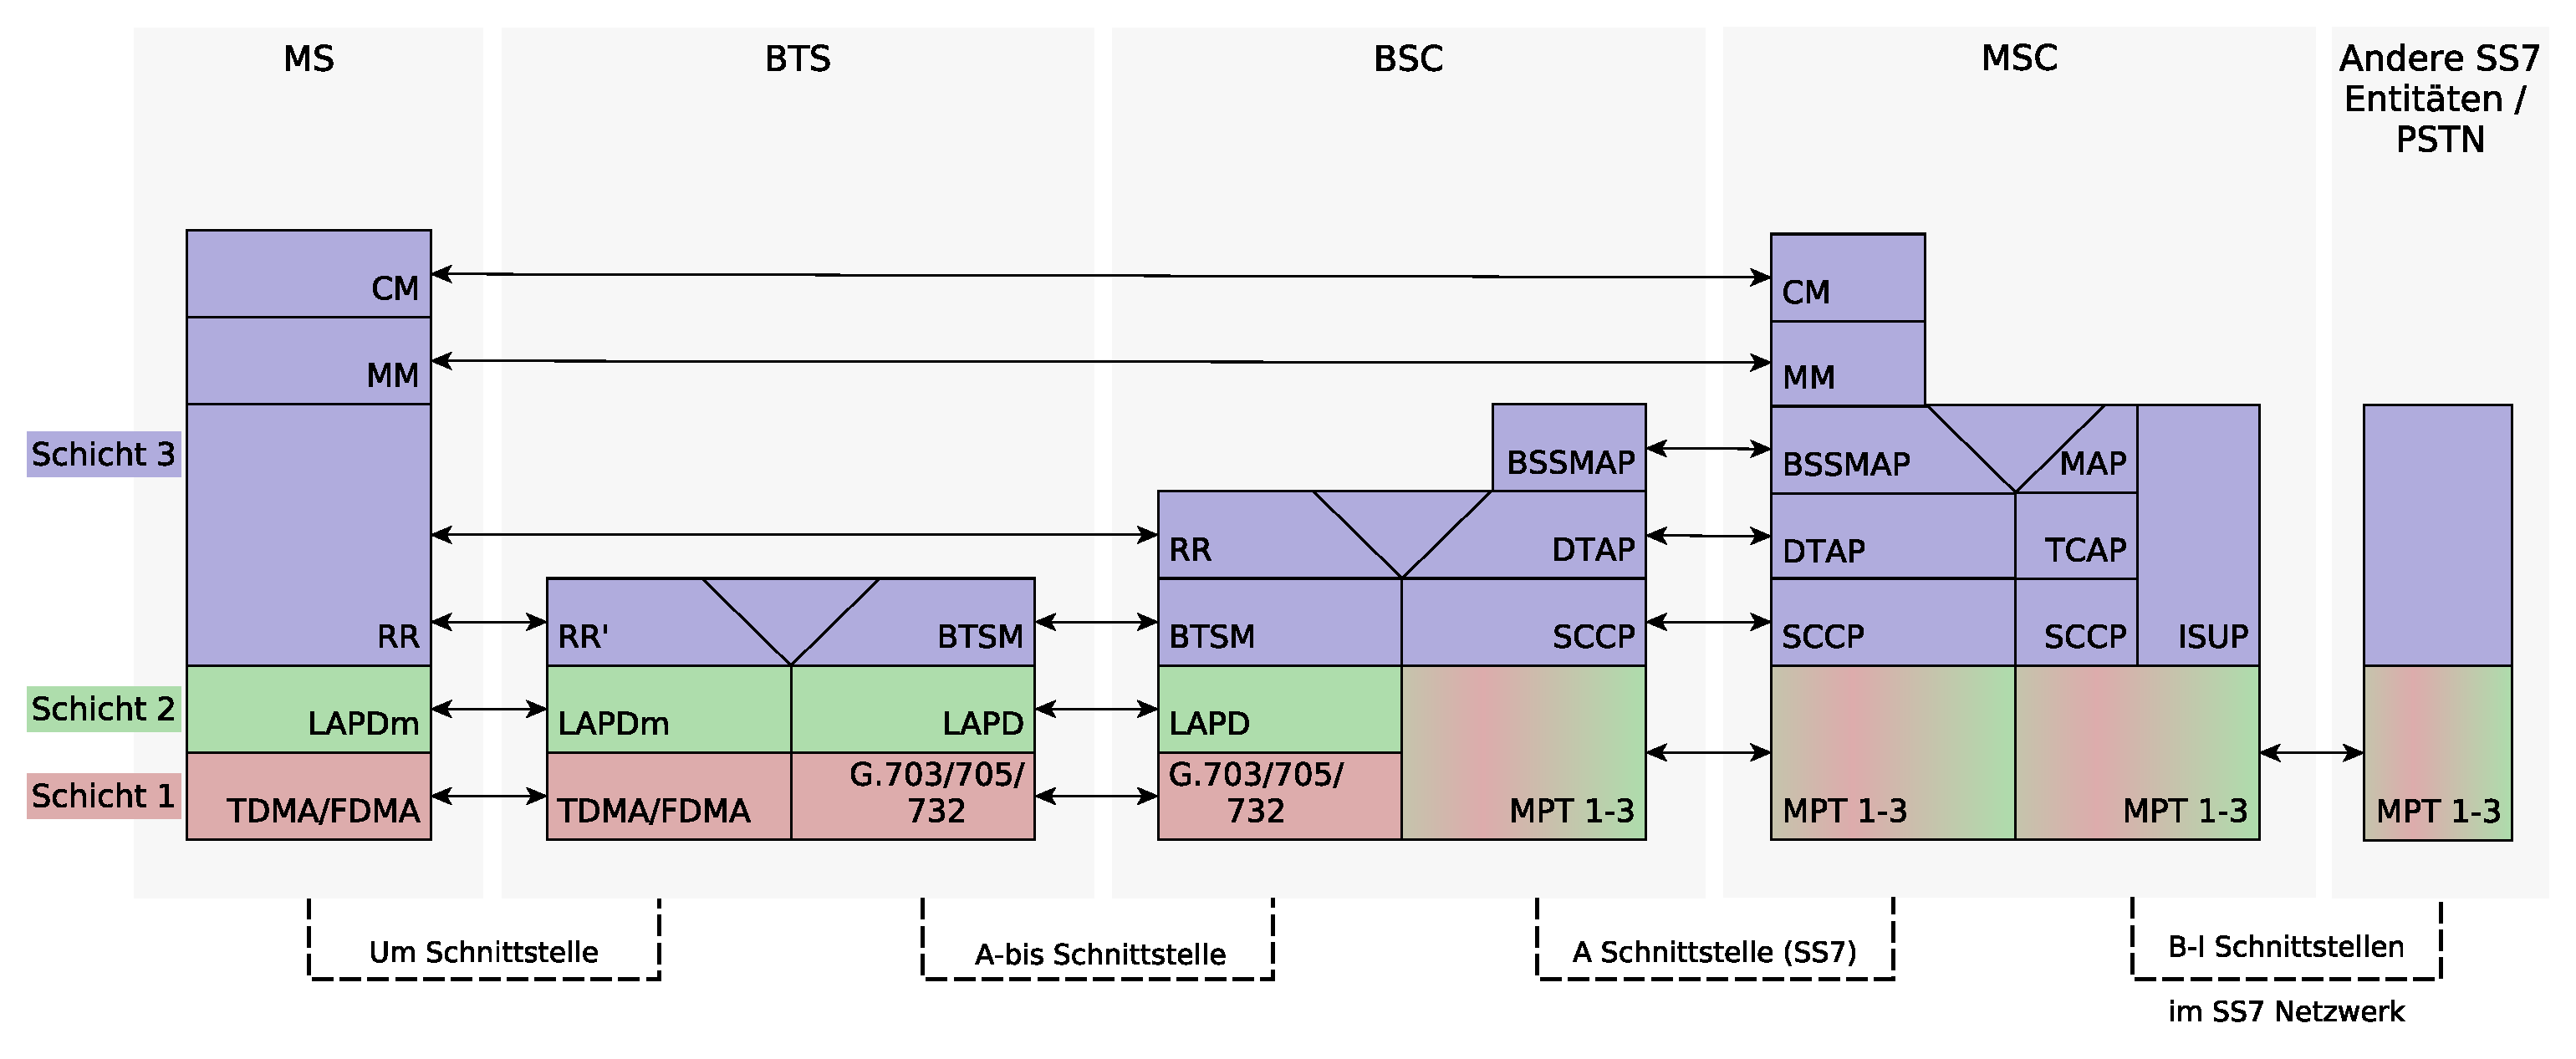
\includegraphics[width=1.0\textwidth]{figures/gsm_protocol_stack.pdf}
  \end{center}
  \caption[Protokollstapel für Signalisierung in GSM]{Protokollstapel für Signalisierung in \ac{GSM}, erstellt mit yEd nach \citep{eberspacher:2008:gsm-architecture}} \label{fig:gsm-protocol-stack} 
\end{figure}

\autoref{fig:gsm-protocol-stack} bietet eine Übersicht über die Signaling Plane, deren Protokollstruktur und Schnittstellen in den folgenden Kapiteln erklärt werden. Hier wegen mangelnder Relevanz nicht erklärte Protokolle und Schnittstellen finden sich im Anhang in \autoref{hdl:a_schnittstellen_protokolle}.

\section{Um Schnittstelle} \label{hdl:einfuehrung-gsm_schnittstellen_protokolle-um_interface}

\acused{Um}

Die Funkschnittstelle zwischen \ac{MS} und \ac{BTS} wird \ac{Um}-Schnittstelle oder auch kurz \ac{Um} genannt. Die Frequenzen für Uplink und Downlink, über die mit einer \ac{BTS} kommuniziert werden kann, werden über die \ac{ARFCN} der \ac{BTS} bestimmt. Auf dem Uplink läuft der Datenfluss Richtung \ac{BTS}, auf dem Downlink Richtung \ac{MS}. Da die Übertragung über die Funkschnittstelle fehlerbehaftet ist, müssen für eine zuverlässige Verbindung Fehlerkorrekturmechanismen implementiert sein.

Das Übertragungsprotokoll der physikalischen Schicht basiert auf einer Kombination aus \ac{FDMA} und \ac{TDMA} (siehe \autoref{hdl:a_tdma_fdma}). Durch \ac{FDMA} wird das verfügbare Frequenzband in verschiedene Trägerfrequenzen unterteilt. Mit \ac{TDMA} werden auf einer Trägerfrequenz acht Zeitschlitze definiert und physikalischen Kanälen zugeteilt. Einem physikalischen Kanal wird durch Multiframes wiederum eine sich wiederholende Sequenz logischer Kanäle zugewiesen. Logische Kanäle bieten verschiedene Funktionen an. Auf \acp{TCH} werden zum Beispiel Sprachdaten, auf \acp{BCCH} Broadcast Signalisierungsdaten und auf \acp{CCCH} Signalisierungsdaten für einzelne Teilnehmer übertragen.

Im Zeitschlitz eines physikalischen Kanals kann genau die Datenmenge eines Bursts übertragen werden. In \autoref{fig:normal_burst} ist der Aufbau eines normalen Bursts dargestellt. Normale Burst werden in \ac{GSM} sowohl für die Übertragung von Nutzdaten auf \acp{TCH}, als auch für die Übertragung von Signalisierungsnachrichten auf \ac{SDCCH}, \ac{SACCH}, \ac{FACCH} und weiteren verwendet. Wie man in der Grafik sehen kann, trägt jeder Burst zwei 57 Bit Datenblöcke auf einmal. Traingssequenz, vorderer und hinterer Tail sind für die Funkübertragung relevant und für diese Arbeit nicht von Bedeutung. Auf die Stealing Flags wird im folgenden Abschnitt eingegangen. Der Aufbau verschiedener Bursttypen kann in \citepauthor[Kap. 5.2.3]{3gpp:05.02} nachgelesen werden.

\begin{figure}[H]
  \begin{center}
    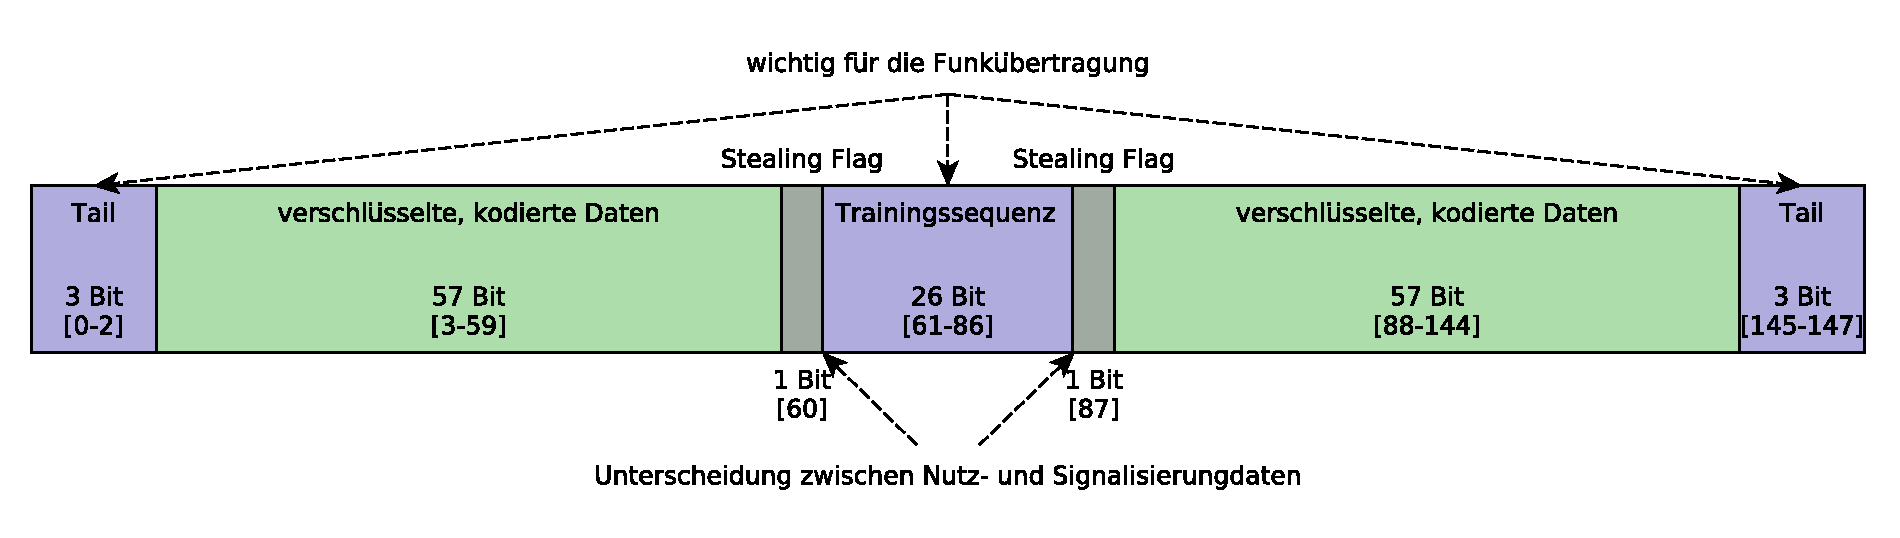
\includegraphics[width=1.0\textwidth]{figures/normal_burst.pdf}
  \end{center}
  \caption[Der Aufbau eines normalen Bursts]{Der Aufbau eines normalen Bursts, erstellt mit yEd nach \citepauthor[Kap. 5.2.3]{3gpp:05.02}} \label{fig:normal_burst} 
\end{figure}

\subsection{Logische Kanäle -- GSM-Multiframe}\label{hdl:logical-channels}

Physikalischen Kanälen können verschiedene Sequenzen logischer Kanäle zugeordnet werden\citepauthor[Kap. 6]{3gpp:04.03}.

Es wird ein sich wiederholendes Multiframe definiert, welches sich auf Signalisierungskanälen nach 51 Frames und auf Datenkanälen nach 26 Frames wiederholt. Die Struktur des Multiframes, also die Sequenz seiner logischen Kanäle, ordnet damit einer Nachricht, über ihre \ac{FN}, genau einem logischen Kanal zu. Durch die unterschiedliche Größe der Multiframes für \ac{TCH}, \ac{BCCH} und \ac{CCCH} beginnen diese erst nach ihrem gemeinsamen Vielfachen ($26 \cdot 51$ Frames) wieder zusammen von vorne -- einem Superframe. Aufgrund der begrenzten Größe der \ac{FN} wird ein Hyperframe von 2048 Superframes definiert, nach der die \ac{FN} wieder bei 0 beginnt \citepauthor[Kap. 6]{3gpp:05.02}. Die \ac{FN} wiederholt sich also alle 3 Stunden, 28 Minuten und 53.76 Sekunden. 

\begin{figure}[H]
  \begin{center}
    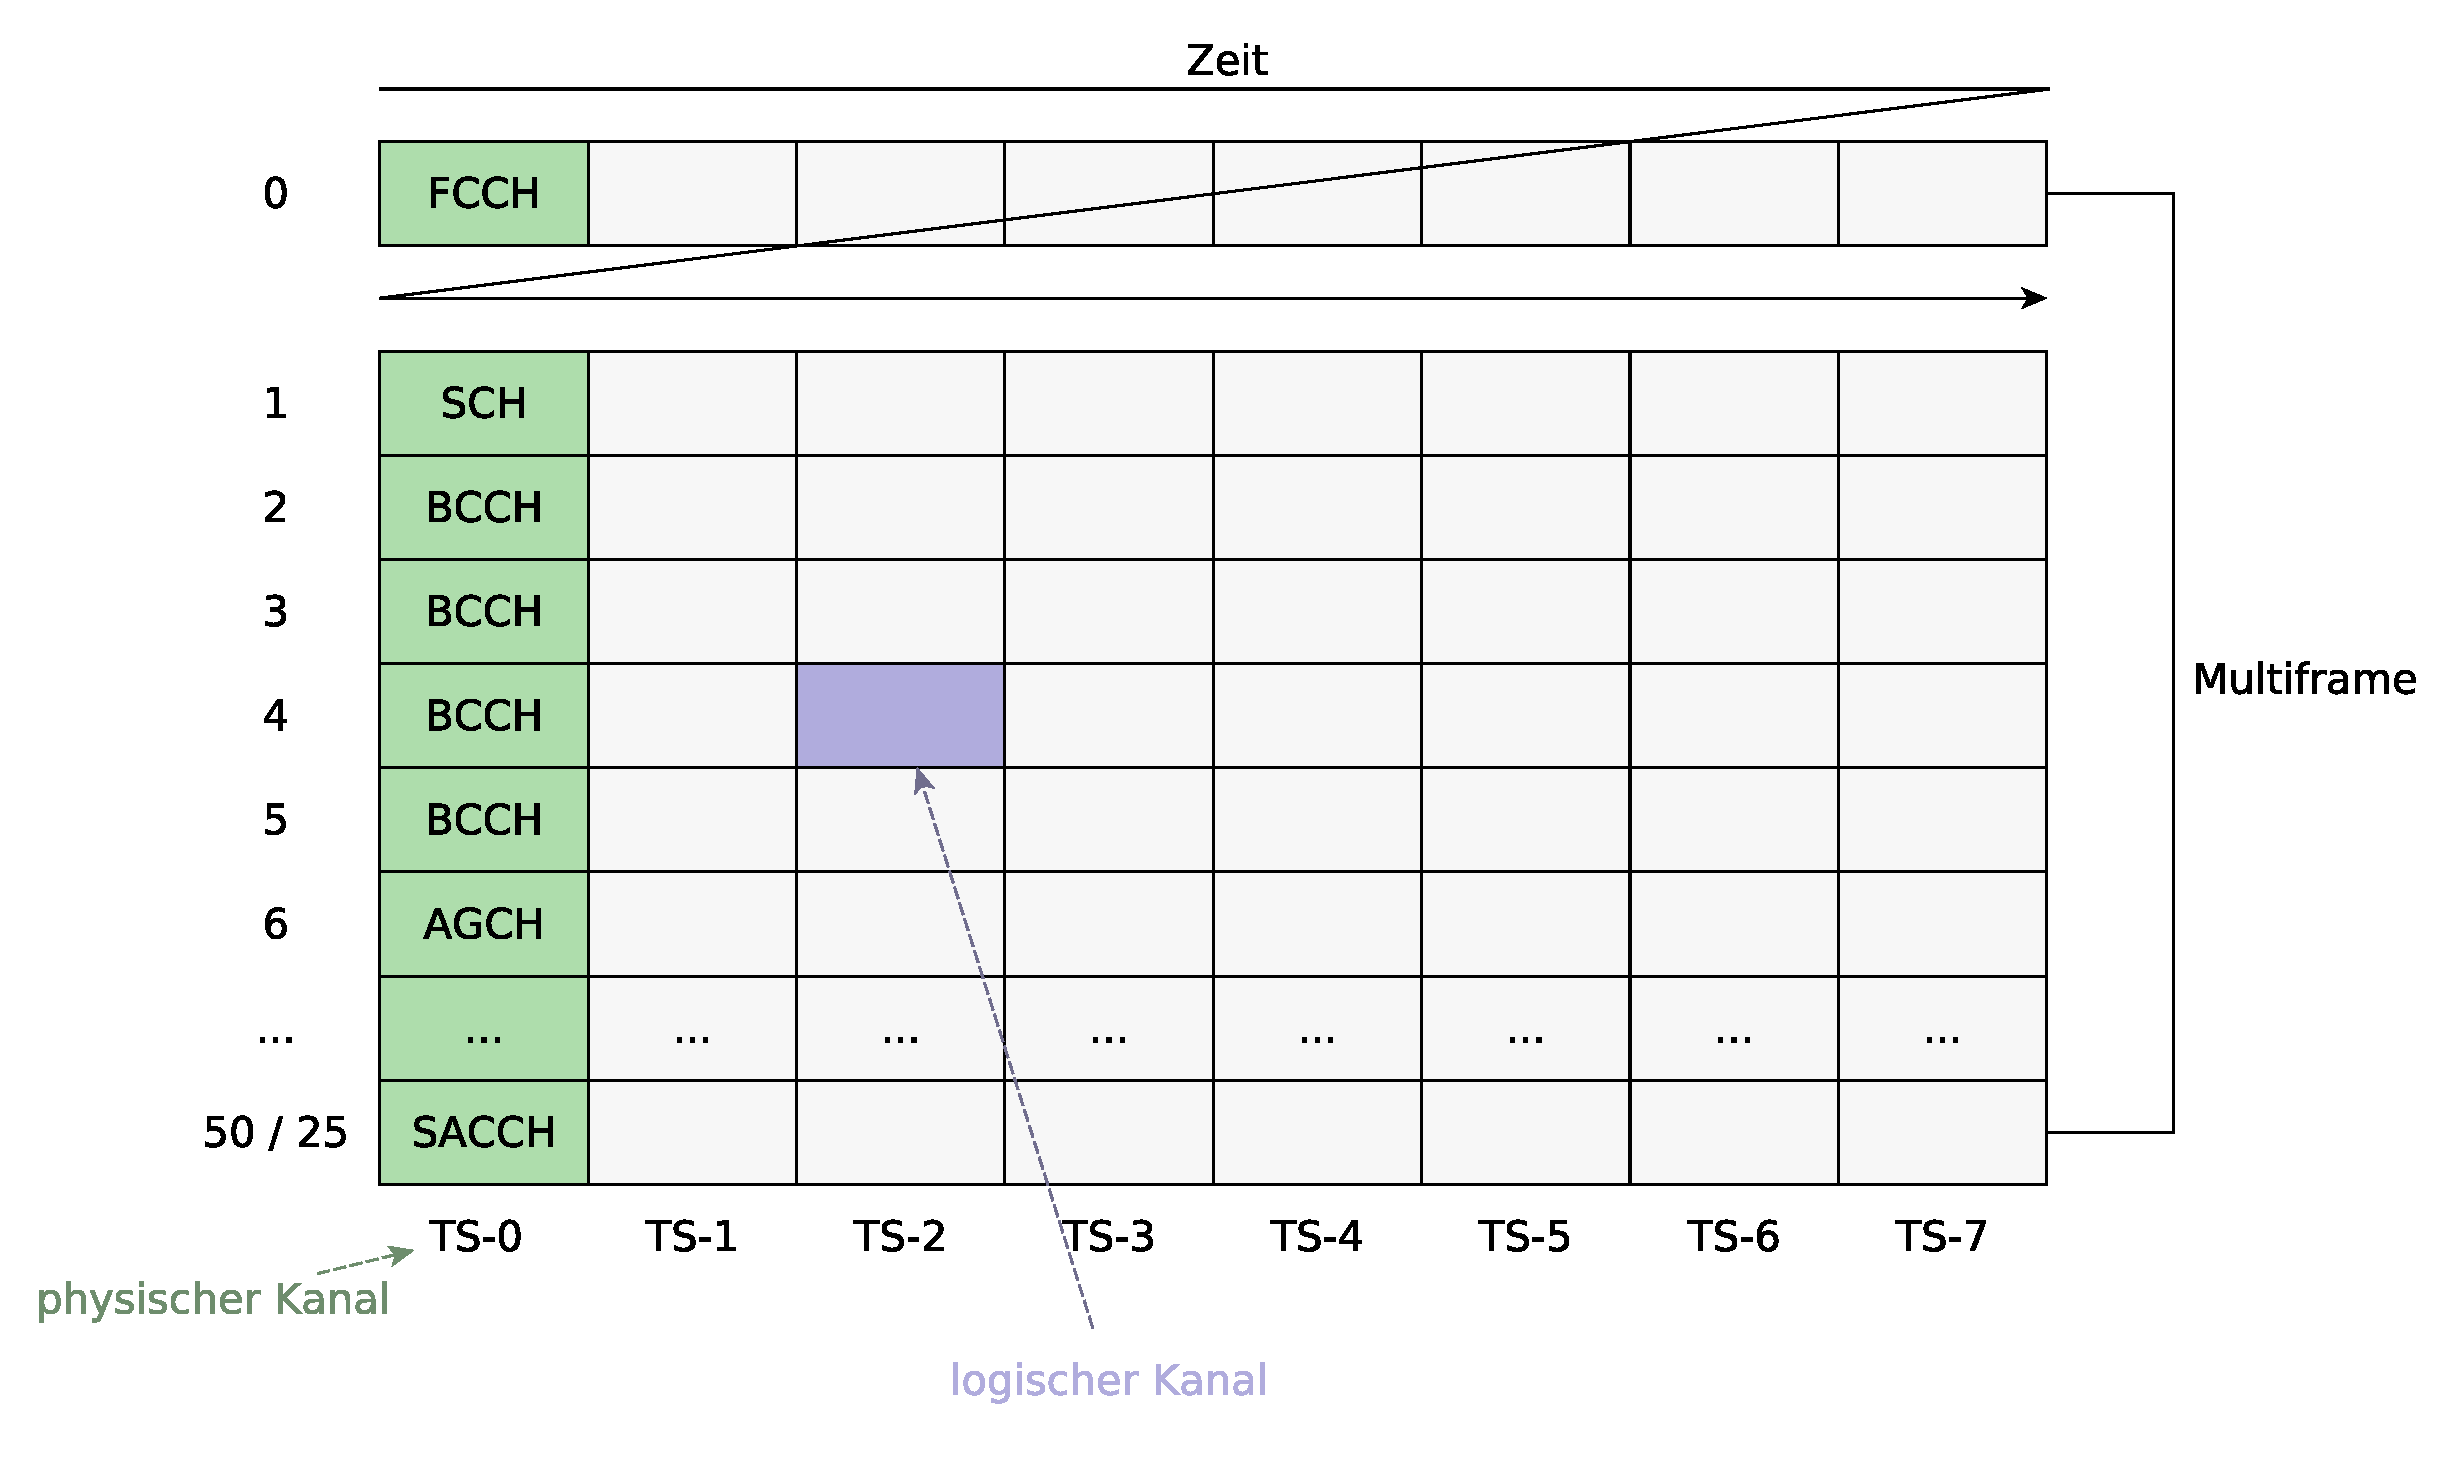
\includegraphics[width=1.0\textwidth]{figures/gsm_multiframe.pdf}
  \end{center}
  \caption[Die GSM Multiframe Struktur]{Die \ac{GSM} Multiframe Struktur, erstellt mit yEd nach \citep[Kap. 1.7.3]{sauter:2011:grundkurs-mobile}} \label{fig:gsm-multiframe} 
\end{figure}

In \ac{GSM} wird jedem physikalischen Kanal ein Multiframe zugeordnet. Das Multiframe, das für die Bestimmung des logischen Kanals einer Nachricht angewendet wird, ist also durch den Zeitschlitz bestimmt, auf dem die Nachricht übertragen wurde. Aus der \ac{FN}, mit der die Nachricht empfangen wurde, wird das Offset im Multiframe berechnet und ihr damit ein logischer Kanal zugeordnet. Die \ac{FN} und der physikalische Kanal bestimmen also eindeutig den logischen Kanal einer Nachricht. \autoref{tab:logical-channels} gibt eine Übersicht über die logischen Kanäle und ihre Funktionen.

Kanäle vom Typ \ac{BCCH}, \ac{CCCH} und \ac{DCCH} übertragen Signalisierungsinformationen und sind Teil der Signaling Plane. Der \ac{TCH} überträgt ausschließlich Sprachdaten und wird der User Plane zugeordnet. Der \ac{SDCCH} wird für Signalisierung und im Fall von \ac{SMS} Nachrichten auch für Nutzdaten verwendet, weshalb durch Multiplexing zwischen User und Signaling Plane unterschieden wird. Für das Multiplexing ist das \ac{SAPI} Feld des \ac{LAPDm} Headers zuständig (siehe \autoref{hdl:einfuehrung-gsm_schnittstellen_protokolle-um_interface-layer2}).

\begin{table}[H]
\begin{adjustbox}{width={1.00\textwidth}, center}
\begin{tabular}{|l|l|l|l|}
\rowcolor[HTML]{F7F7F7} 
\hline
\textbf{Name} & \textbf{Beschreibung}                 	& \textbf{Richtung} & \textbf{Typ} 	\\ \hline
\acs{BCCH}          & \acl{BCCH}              			& Downlink          & Broadcast    		\\ \hline
\acs{SCH}           & \acl{SCH}               			& Downlink          & Broadcast   		\\ \hline
\acs{FCCH}          & \acl{FCCH}        			  	& Downlink          & Broadcast    		\\ \hline
\acs{AGCH}          & \acl{AGCH}                  		& Downlink          & Common Control       		\\ \hline
\acs{PCH}           & \acl{PCH}                         & Downlink          & Common Control       		\\ \hline
\acs{RACH}          & \acl{RACH}                 		& Uplink            & Common Control       		\\ \hline
\acs{FACCH}         & \acl{FACCH}       				& Bidirektional     & Dedicated Control    		\\ \hline
\acs{SACCH}         & \acl{SACCH}       				& Bidirektional     & Dedicated Control    		\\ \hline
\acs{SDCCH}         & \acl{SDCCH} 						& Bidirektional     & Dedicated Control    		\\ \hline
\acs{TCH}           & \acl{TCH}                       	& Bidirektional     & Nutzdatenkanal  \\ \hline
\end{tabular}
\end{adjustbox}
\caption{Die logischen Kanäle der Funkschnittstelle}\label{tab:logical-channels}
\end{table}
\acused{BCCH}\acused{SCH}\acused{FCCH}\acused{AGCH}\acused{PCH}\acused{RACH}\acused{FACCH}\acused{SACCH}\acused{SDCCH}\acused{TCH}

\textbf{\acfp{BCCH}} werden für Nachrichten von der \ac{BTS} an alle sich im Empfangsbereich befindenden \acp{MS} verwendet. Es gibt sie deshalb nur im Downlink. \citepauthor[Kap. 4.1.1]{3gpp:04.03}
\begin{itemize}
\item \textbf{\ac{BCCH}}: Auf dem \ac{BCCH} werden über die \ac{SI} Nachrichten regelmäßig Konfiguration und Parameter des Netzwerks verschickt. Davon gibt es insgesamt 9, von denen aber nur \ac{SI}-1 bis \ac{SI}-4 auf dem \ac{BCCH} übertragen werden.
\item \textbf{\ac{SCH}}: Die auf diesem Kanal gesendeten Bursts ermöglichen es Endgeräten, sich mit der Multiframe-Struktur der \ac{BTS} zu synchronisieren. Damit das \ac{MS} den Burst dekodieren kann, obwohl es zu diesem Zeitpunkt die Entfernung und damit den genauen Anfang des empfangenen Bursts nicht kennt, haben die Synchronisation-Bursts ein spezielles Format.
\item \textbf{\ac{FCCH}}: Dieser Kanal dient zur Kalibrierung des Transceivers der \ac{MS} und definiert den Anfang des Multiframes.
\end{itemize}

Auf den \textbf{\acfp{CCCH}} werden Signalisierungsinformationen ausgetauscht, mit denen dedizierte bidirektionale Kanäle beantragt und vergeben werden können. Die \acp{CCCH} werden von mehreren \acp{MS} verwendet. \citepauthor[Kap. 4.1.2]{3gpp:04.03}
\begin{itemize}
\item \textbf{\ac{RACH}}: Auf dem einzigen Kanal den es nur im Uplink gibt, können \acp{MS} mit einem sogenannten "`Channel Request"' vom Netzwerk einen dedizierten Kanal anfordern.
\item \textbf{\ac{AGCH}}: Der \ac{AGCH} wird verwendet, um einer \ac{MS} nach einem Channel-Request einen dedizierten Kanal zuzuweisen.
\item \textbf{\ac{PCH}}: Auf dem \ac{PCH} werden \acp{MS} im Empfangsbereich einer Basisstation über eingehende Anrufe und \ac{SMS} informiert.
\end{itemize} 

Die bidirektionalen \textbf{\acfp{DCCH}} sind einer dedizierten Verbindung zwischen \ac{BTS} und \ac{MS} zugeordnet. Um sie vor Zugriff von anderen zu schützen wird der Datentransfer auf \acp{DCCH} in der Regel verschlüsselt. \citepauthor[Kap. 4.1.3]{3gpp:04.03}
\begin{itemize}
\item \textbf{\ac{FACCH}}: Der \ac{FACCH} ist ein Signalisierungskanal, der auf einem \ac{TCH} übertragen wird. Er wird für dringende Signalisierungsnachrichten verwendet, wobei die Nutzdaten des Bursts durch Signalisierungsinformationen ersetzt werden. Ob der \ac{TCH}-Burst vom \ac{FACCH} gestohlen wurde, wird durch Setzen eines "`Stealing Flags"' gekennzeichnet. Der Qualitätsverlust der Sprachübertragung durch die fehlenden Nutzdaten ist nicht hörbar.
\item \textbf{\ac{SACCH}}: Der \ac{SACCH} wird im Uplink für die Übertragung von Messdaten, wie der Signalstärke benachbarter \ac{BTS}, verwendet. Im Downlink erhält die \ac{MS} Befehle zu Leistungsregelung von der \ac{BTS}. 
\item \textbf{\ac{SDCCH}}: Der \ac{SDCCH} wird für die Signalisierung bei der Nutzung von Netzdiensten verwendet, zum Beispiel für den Aufbau eines Gesprächs, das Einrichten einer verschlüsselten Verbindung, Identitätsabfragen, Authentifizierung und "`Location Updates"'. Freie Kapazitäten werden für den Empfang und Versand von \ac{SMS} Nachrichten benutzt. In diesem Fall dient er auch der Übertragung von Nutzdaten.
\end{itemize}

Der \textbf{\ac{TCH}} ist ein bidirektionaler, dedizierter Nutzdatenkanal, über den entweder Sprachdaten oder leitungsvermittelte Datendienste übertragen werden.

\subsection{Service Access Point}\label{hdl:sap}

Ein \ac{SAP} ist eine interne Schnittstelle zwischen Protokollschichten. Die Kommunikation zwischen den Schichten basiert dabei, wie in \ac{GSM} üblich, auf Primitives. Es gibt folgende Typen von Primitives \citepauthor{3gpp:04.04}:

\begin{itemize}
\item \textbf{\ac{IND}}: Layer 1 $\rightarrow$ Layer 2+\\
Benachrichtigung höherer Schichten über Vorkommnisse auf dieser Schicht -- wie zum Beispiel eingehende Daten.
\item \textbf{\ac{REQ}}: Layer 1 $\leftarrow$ Layer 2+\\
Höhere Schichten können damit vom \ac{SAP} angebotene Dienste nutzen.
\item \textbf{\ac{RES_proto}}: Layer 1 $\leftarrow$ Layer 2+\\
Bestätigung des Empfangs einer Indication.
\item \textbf{\ac{CON}}: Layer 1 $\rightarrow$ Layer 2+\\
Antwort auf Response nach erfolgreich abgearbeiteter Routine.
\end{itemize}

Folgende Abbildung aus \citetauthor{3gpp:04.04} zeigt die Schnittstellen der physikalischen Schicht in \ac{GSM} zu anderen Protokollschichten. Die physikalische Schicht bietet \ac{SAP}-Schnittstellen zur Datensicherungsschicht und dem Schicht 3 zugeordneten \ac{RR}-Management, die über PH-Primitives und MPH-Primitives angesprochen werden können.

\begin{figure}[H]
  \begin{center}
    \includegraphics[width=0.8\textwidth]{figures/0404_fig_21.pdf}
  \end{center}
  \caption[Die Schnittstellen der physikalischen Schicht]{Die Schnittstellen der physikalischen Schicht, aus \citepauthor[Abb. 2.1]{3gpp:04.04}} \label{fig:interface-physical-layer} 
\end{figure}

Die logischen Kanäle definieren im Fall der physikalischen Schicht unterschiedliche \acp{SAP} zu \ac{LAPDm}, wie in \autoref{fig:sap-logical-channels} zu sehen ist.

\begin{figure}[H]
  \begin{center}
    \includegraphics[width=0.95\textwidth]{figures/0404_fig_23.pdf}
  \end{center}
  \caption[SAPs der physikalischen Schicht zur Sicherungsschicht ]{\acp{SAP} der physikalischen Schicht zur Sicherungsschicht, aus \citepauthor[Abb. 3.2]{3gpp:04.04}} \label{fig:sap-logical-channels} 
\end{figure}


\subsection{Link Access Protocol Dm-Channel}
\label{hdl:einfuehrung-gsm_schnittstellen_protokolle-um_interface-layer2}

Die Aufgabe des in \citetauthor{3gpp:04.05} und \citetauthor{3gpp:04.06} spezifizierten \ac{LAPDm}-Protokolls der Datensicherungsschicht ist der Aufbau einer zuverlässigen Verbindung zwischen \ac{MS} und \ac{BTS}. Für die zuverlässige Übertragung von Daten stellt es einen \ac{SAP} für Schicht 3 zur Verfügung, selbst greift es auf die von der physikalischen Schicht angebotenen \acp{SAP} der logischen Kanäle zu (siehe \autoref{fig:sap-logical-channels}). Das zwischen \ac{MS} und \ac{BTS} terminierende Protokoll wurde in großen Teilen aus der \ac{ISDN}-Spezifikation des Protokolls \ac{LAPD} übernommen und an die Anforderungen der Funkschnittstelle angepasst. 

Das Protokoll soll mehrere Einheiten von physikalischer Schicht und Schicht 3 unterstützen, sowie die Signalisierung auf \ac{BCCH}, \ac{CCCH} und \ac{DCCH}. In \citetauthor[Kap. 3.1]{3gpp:04.05} wird sein Funktionsumfang wie folgt beschrieben:

\begin{itemize}
\item Unterstützung einer oder mehrerer Schicht 3 Datenverbindungen, die durch einen \ac{DLCI} identifiziert werden.
\item Unterscheidung verschiedener Nachrichtentypen.
\item Transparente Nachrichtenübertragung zwischen Schicht 3 Einheiten.
\item Sicherstellen der korrekten Reihenfolge der Nachrichten (Ablaufsteuerung).
\item Anpassen der Datenrate an Eigenschaften der physikalischen Schicht (Flusskontrolle).
\item Benachrichtigung von Schicht 3 Einheiten über nicht behebbare Fehler. 
\end{itemize}

\ac{LAPDm} bietet Schicht 3 zwei verschiedenen Übertragungsoperationen an. Die unzuverlässige "`unacknowledged operation"' und die zuverlässige "`acknowledged operation"'. Auf \ac{BCCH} und \ac{CCCH} ist nur die unzuverlässige Operation verfügbar, auf \ac{DCCH} können beide benutzt werden. Mit den beiden Übertragungstypen realisiert \ac{LAPDm} die Dienste "`Unacknowledged Information Transfer"' für unzuverlässige und "`Acknowledged Multiple Frame Information Transfer"' für zuverlässige Datenverbindungen.

\subsubsection*{Unacknowledged Information Transfer}

Von Schicht 2 wird weder die korrekte Reihenfolge verifiziert, noch dass eine gesendete Nachricht beim Empfänger angekommen ist \citepauthor[Kap. 4.2.4]{3gpp:04.05}. Nachrichten werden als \ac{UI}-Frames übertragen. 

\subsubsection*{Acknowledged Multiple Frame Information Transfer}
\acused{N(R)}\acused{N(S)}\acused{RRm}

Durch Kontrollmechanismen von Schicht 2 wird sichergestellt, dass übertragene Daten in der richtigen Reihenfolge beim Empfänger ankommen \citepauthor[Kap. 4.2.5]{3gpp:04.05}. Auf beiden Seiten werden jeweils die Nummern \ac{N(R)} empfangener und \ac{N(S)} gesendeter Nachrichten gepflegt. Die übertragenen \ac{I}-Frames enthalten diese beiden Zähler. Durch Synchronisation der empfangenen Nummern mit den eigenen kann so festgestellt werden, ob Daten verloren gegangen sind oder die Reihenfolge nicht mehr stimmt. Mit einer \ac{REJ} Nachricht kann eine fehlerhaft empfangene Nachricht abgewiesen werden, mit Receive-Ready (\acs{RRm})-Nachrichten wird der Gegenseite mitgeteilt, welche Nachricht sie als nächstes schicken soll. Ein \ac{RRm} enthält dazu die Nummer $\ac{N(R)} + 1$ und bestätigt gleichzeitig den Empfang aller Nachrichten bis zu dieser. Sollte die Datensicherungsschicht keine Möglichkeit haben eine zuverlässige Verbindung zu gewährleisten, wird ein Fehler an Schicht 3 gemeldet. Mit einer \ac{SABM}-Nachricht signalisiert Schicht 2 ihrer Gegenseite, dass in den zuverlässigen Übertragungsmodus gewechselt werden soll. Diese bestätigt den Wechsel mit einer \ac{UA}-Nachricht. Mit einem \ac{DISC} kann von beiden Seiten die Verbindung wieder beendet und in den unzuverlässigen Modus gewechselt werden \citepauthor[Kap. 5.4]{3gpp:04.06}.

\subsubsection*{Aufbau eines LAPDm-Frames} \label{hdl:lapdm-format}

Für \ac{LAPDm}-Nachrichten auf verschiedenen logischen Kanälen werden auch verschiedene Formate definiert. Da für die Masterarbeit nur \ac{LAPDm} Nachrichten auf \ac{DCCH} untersucht werden, wird hier nur auf das "`Frame Format A"' eingegangen. Dieses ist, wie auch die anderen Formate, in \citetauthor[Kap. 2]{3gpp:04.06} definiert.

\begin{figure}[H]
	\centering \includegraphics[width=0.9\linewidth]{figures/0406_fig_1_pt_1.pdf}
	\caption[Das LAPDm Format A]{Das \ac{LAPDm} Format A, aus \citep[Abb. 1, Teil 1]{3gpp:04.06}} \label{fig:lapdm-format-a}
\end{figure}

Obige Abbildung zeigt die \ac{LAPDm}-Nachricht im Format A. Sie setzt sich aus je einem Byte (Oktett) für Adressierungs-, Kontroll- und Längeninformationen und N201 Bytes an Nutzdaten zusammen. Die Größe von N201 wird in \citetauthor[Kap. 5.8.3]{3gpp:04.06} für \ac{FACCH} und \ac{SDCCH} als 20 definiert, damit ist die gesamte Nachricht 23 Bytes oder 184 Bit lang. 

\begin{figure}[H]
	\centering \includegraphics[width=0.8\linewidth]{figures/0406_fig_4.pdf}
	\caption[Das LAPDm Addressierungsfeld]{Das \ac{LAPDm} Addressierungsfeld, aus \citep[Abb. 4]{3gpp:04.06}} \label{fig:lapdm-format-addr}
\end{figure}

Das oben gezeigte Adressierungsfeld liefert Informationen über den Sender und Empfänger der Nachricht. Das \ac{EA} sagt aus, ob dies das letzte Byte des Adressierungsfeldes ist oder noch weitere folgen. Es wird benötigt, da das Adressierungsfeld auch mehrere Bytes lang sein kann. Das \ac{C/R} definiert ob es sich um einen Befehl (Command) oder die Antwort auf diesen (Response) handelt. Die \ac{SAPI} entspricht dem \ac{DLCI} und definiert die Schicht 3 Datenverbindung, für die die Nachricht bestimmt ist. Das \ac{LPD}-Feld identifiziert das verwendete Schicht 2 Protokoll und ist in \ac{LAPDm} immer 0.

\begin{figure}[H]
	\centering \includegraphics[width=0.8\linewidth]{figures/0406_tab_3.pdf}
	\caption[Das LAPDm Kontrollfeld]{Das \ac{LAPDm} Kontrollfeld, aus \citep[Tabelle 3]{3gpp:04.06}} \label{fig:lapdm-format-ctl}
\end{figure}

Der oben gezeigte Aufbau des Kontrollfelds hängt mit dem verwendeten Nachrichtenformat zusammen. Beim nummerierten \ac{I}-Format (Bit[1] == 0) gibt es die Nummer der letzten korrekt empfangenen Nachricht \ac{N(R)} und die Nummer der zuletzt gesendeten Nachricht \ac{N(S)}. Das \ac{S} (Bit[1,2] == 10) benötigt die Nummer \ac{N(R)} der erwarteten nächsten Nachricht und zwei S-Bits, die die verwendete Supervisory Funktion (zum Beispiel \ac{RRm}) bestimmen. Das \ac{U} (Bit[1,2] == 11) ist nicht durchnummeriert und benutzt alle U-Bits für die Bestimmung der verwendeten Unnumbered Funktion (zum Beispiel \ac{SABM}). Das \ac{P/F} definiert bei einem Command, ob man eine Antwort der Gegenseite möchte und bei einer Response, ob es sich um eine Antwort auf einen "`Poll"' der Gegenseite handelt.

\begin{figure}[H]
	\centering \includegraphics[width=0.9\linewidth]{figures/0406_fig_5.pdf}
	\caption[Das LAPDm Längeninformationsfeld]{Das \ac{LAPDm} Längeninformationsfeld, aus \citep[Abb. 5]{3gpp:04.06}} \label{fig:lapdm-format-len}
\end{figure}

Das \ac{EL} der oben gezeigten Längeninformation sagt aus, ob es sich bei diesem um das letzte Byte handelt (siehe \ac{EA} im Adressierungsfeld). Das \ac{M} zeigt an, ob sich die übertragene Signalisierungsnachricht aus mehr als dieser \ac{LAPDm}-Nachricht zusammensetzt. Das wird benötigt, wenn mehr als 160 Bit an Signalisierungsinformationen übertragen werden müssen, da diese nicht mehr in eine einzelne \ac{LAPDm}-Nachricht passen. Der \ac{L} gibt die Länge der Nutzdaten in dieser Nachricht an. Alle Daten nach der definierten Länge enthalten keine nützlichen Information mehr und werden in der Regel mit \texttt{0x2b} aufgefüllt.

\section{Schicht 3 Protokolle}

Die Protokollebene 3 besteht in \ac{GSM} aus \acf{RR}, \acf{MM} und \acf{CM}, die verschiedene Aufgaben übernehmen. Ein Teil des \ac{RR}-Protokolls fällt in den Aufgabenbereich der \ac{BTS} und wird von dieser bearbeitet, der Rest wird transparent an den \ac{BSC} weitergeleitet. \ac{MM} und \ac{CM} werden weder von \ac{BTS} noch \ac{BSC} bearbeitet und den Protokollen zugewiesene Nachrichten zwischen \ac{MS} und \ac{MSC} ausgetauscht. Der für die Funkschnittstelle relevante Teil der Protokolle ist in \citetauthor{3gpp:04.18} spezifiziert, der Rest findet sich in \citetauthor{3gpp:24.008} und \citetauthor{3gpp:23.108}.

\begin{figure}[H]
	\centering \includegraphics[width=0.9\linewidth]{figures/24008_fig_10-1.pdf}
	\caption[Der gemeinsame Header der Schicht 3 Protokolle]{Der gemeinsame Header der Schicht 3 Protokolle, aus \citep[Abb. 10.1]{3gpp:24.008}} \label{fig:l3-common-hdr}
\end{figure}

Die Protokolle teilen sich den in \autoref{fig:l3-common-hdr} gezeigten, gemeinsamen Header \citep[11.2.3.1]{3gpp:24.007}. Bit 1 bis 4 werden einem Protokolldiskriminator zugeordnet und ermöglichen die Unterscheidung der verschiedenen Schicht 3 Protokolle. Die für die Arbeit relevanten Werte für diesen sind in \autoref{tab:l3-prot-disc-values} aufgeführt. Bit 5 bis 8 kann entweder unbenutzt bleiben und übersprungen werden ("`Skip Indicator"') oder für die Zuordnung der Nachricht zu einer von bis zu 16 Transaktionen oder Verbindungen (\ac{TI}) verwendet werden. Das zweite Byte ist für den Typ der übertragenen Nachricht reserviert ("`Message Type"'), von denen die Schicht 3 Protokolle verschiedene spezifizieren können. 

\begin{table}[H]
\centering
\begin{tabular}{|l|l|}
\hline
Bits 4 3 2 1 & Protokoll                 \\ \hline
0 0 1 1      & Call Control              \\ \hline
0 1 0 1      & Mobility Management       \\ \hline
0 1 1 0      & Radio Resource Management \\ \hline
1 0 0 1      & SMS                       \\ \hline
\end{tabular}
\caption[Werte des Schicht 3 Protokolldiskriminators]{Werte des Schicht 3 Protokolldiskriminators, nach \citep[Tabelle 11.2]{3gpp:24.007}}
\label{tab:l3-prot-disc-values}
\end{table}

Die Informationsfelder des Schicht 3 Headers sind im \ac{TLV} Format angegeben. Der "`Type"' ist der \ac{IEI} des Informationselements, "`Length"' seine Länge und "`Value"' sein Wert. Damit ist es möglich, optionale Informationselemente dynamischer Länge aneinanderzureihen. Ist die Position des Feldes festgelegt, muss T nicht mit angegeben werden. Ist die Länge festgelegt, muss L nicht angegeben werden. Bei einem reinen V Feld sind zum Beispiel sowohl Länge als auch Typ festgelegt. \autoref{tab:tlv-ie} zeigt die Kombinationsmöglichkeiten.

\begin{table}[H]
\centering
\begin{tabular}{|l|l|l|l|l|}
\hline
             & \textbf{T (Typ)} & \textbf{L (Länge)} & \textbf{V (Wert)} & \textbf{Gesamtlänge} \\ \hline
\textbf{V}   & -                & -                  & +                 & fest                 \\ \hline
\textbf{T}   & +                & -                  & -                 & fest                 \\ \hline
\textbf{TV}  & +                & -                  & +                 & fest                 \\ \hline
\textbf{LV}  & -                & +                  & +                 & dynamisch            \\ \hline
\textbf{TLV} & +                & +                  & +                 & dynamisch            \\ \hline
\end{tabular}
\caption[Das TLV Format für Informationselemente der Protokollschicht 3]{Das \ac{TLV} Format für Informationselemente der Protokollschicht 3, nach \citepauthor[Kap. 11.2.1.1]{3gpp:24.007}}
\label{tab:tlv-ie}
\end{table}

Im Folgenden wird näher auf die \ac{RR}, \ac{MM} und \ac{CM}-Protokolle eingegangen. 

\subsection{\acl{RR}}
\acf{RR} ist größtenteils für die Verwaltung der Frequenzen und Kanäle zuständig. Die Kommunikation dazu läuft zwischen den \ac{RR}-Modulen von \ac{MS} und \ac{BSC}. Zwischen \ac{MS} und \ac{BTS} terminiert die Messung der Verbindungsqualität auf der Funkschnittstelle und die Regelung der Signalstärken der \ac{MS}. Das Einrichten, Aufrechterhalten und Beenden von \ac{RR}-Verbindungen, die eine dedizierte Verbindung zwischen \ac{MS} und Netzwerk ermöglichen, ist die Hauptaufgabe von \ac{RR} [\citetauthor{3gpp:04.18}].

Übersicht über die Aufgaben des \ac{RR} im \ac{MS} \citepauthor[Kap. 3.2.1]{3gpp:04.18}:
\begin{itemize}
\item \ac{BCCH}-Überwachung: Die Auswertung von \ac{SI}-Nachrichten auf dem Downlink.
\item \ac{PCH}-Überwachung: Die Auswertung von Paging-Nachrichten auf dem Downlink.
\item \ac{RACH}-Verwaltung: Das Anfordern eines dedizierten Signalisierungskanals als Antwort auf Paging oder initiiert vom \ac{MS}.
\item Der Aufbau von \ac{RR}-Verbindungen auf dedizierten Kanälen.
\item Der Transport von Nachrichten über \ac{RR}-Verbindungen.
\item Das Aushandeln von Verschlüsselungsalgorithmen und die Einrichtung verschlüsselter Verbindungen.
\item Die Messung und Mitteilung der Verbindungsqualität an die \ac{BTS}.
\end{itemize}

Übersicht über die Aufgaben des \ac{RR} im Netzwerk \citepauthor[Kap. 3.2.2]{3gpp:04.18}:
\begin{itemize}
\item Die Zuweisung und der Aufbau von \ac{RR}-Verbindungen auf dedizierten Kanälen.
\item Der Transport von Nachrichten über \ac{RR}-Verbindungen.
\item Das Aushandeln von Verschlüsselungsalgorithmen und die Einrichtung verschlüsselter Verbindungen.
\item Die Überwachung der Verbindungsqualität der \acp{MS} und die Regelung von deren Sendeleistung.
\item Die Durchführung von Handover-Prozeduren, also die Übergabe von laufenden Gesprächen zwischen \ac{BSC} oder \ac{BTS}, wenn sich ein \ac{MS} in einen neuen Zuständigkeitsbereich begibt.
\end{itemize}

\subsection{\acl{MM}}
\acf{MM} ist für alle Funktionen und Abläufe zuständig, die sich aus der Mobilität des Mobilfunkteilnehmers ergeben. Die komplette \ac{MM}-Signalisierung läuft transparent für das \ac{BSS}, zwischen \ac{MSC} und \ac{MS}, ab. Für die Nachrichtenübertragung greift das \ac{MM} über einen \ac{SAP} auf die vom \ac{RR} zur Verfügung gestellte, dedizierte Verbindung zu. Das Protokoll ist in \citetauthor{3gpp:24.008} spezifiziert, Beispiele für die Abläufe finden sich in \citetauthor{3gpp:23.108}.

Übersicht über die Aufgaben des \ac{MM} \citepauthor[Kap. 4]{3gpp:24.008}:
\begin{itemize}
\item Die Zuweisung von \acp{TMSI} zum Schutz der Teilnehmeridentitäten.
\item Die Lokalisierung der \ac{MS} im \ac{BSS}, also die Bearbeitung von "`Location Updates"'.
\item Die Zuordnung von \acp{IMSI} und \acp{IMEI} zu \ac{MS}.
\item Die Authentifizierung von Netzteilnehmern.
\item Die Registrierung ("`\ac{IMSI}-Attach"') und Abmeldung ("`\ac{IMSI}-Detach"') von Netzteilnehmern beim Einlegen und Entfernen der \ac{SIM}-Karte.
\end{itemize}

\subsection{\acl{CM}}
\acf{CM} ist für den Aufbau von Verbindungen zwischen Endgeräten zuständig, dazu gehören Telefonate und der Versand von \ac{SMS}. \ac{CM} wird noch einmal unterteilt in \acf{CC}, \acf{SS} und \ac{SMS}. Ebenso wie beim \ac{MM} sind Nachrichten des \ac{CM} transparent für das \ac{BSS} \citepauthor{3gpp:24.007}.

Übersicht über die Aufgaben des \ac{CM}:
\begin{itemize}
\item \ac{CC} kümmert sich um den Aufbau, die Verwaltung und das Beenden von Anrufen \citepauthor[Kap. 5]{3gpp:24.008}.
\item \ac{SS} kann anrufbezogen sein oder nicht. Der anrufbezogene Teil ist zuständig für Anrufweiterleitung, Halten und Warten, sowie Gruppenanrufe \citepauthor{3gpp:24.010}.
\item \begin{sloppypar}\ac{SMS} regelt den Empfang und Versand von "`Point-to-Point"' Kurznachrichten \citepauthor{3gpp:24.011}.\end{sloppypar}
\end{itemize}

\section{Signalverarbeitung und Kanalkodierung} \label{hdl:encoding}
Die im \ac{DSP} meist in Hardware implementierte Logik für digitale Signalverarbeitung, Kodierung und Verschlüsselung von Daten wird der physikalischen Schicht zugeordnet. \autoref{fig:gsm-signal-processing} zeigt, welche Schritte Sprachdaten und sonstige digitale Daten durchlaufen, bevor sie als analoges Signal auf der Trägerfrequenz gesendet werden. Im Gegensatz zu anderen digitalen Daten durchläuft Sprache noch einen zusätzlichen Kodierungsschritt. Sprachkodierungen wie Full-Rate-, Half-Rate-, Enhanced-Full-Rate und Adaptive-Multi-Rate-Speech-Codec sorgen für eine verlustbehaftete Kompression der Sprachdaten, um die benötigte Bandbreite zu reduzieren. \citep[S. 55 ff.]{sauter:2011:grundkurs-mobile}.

\begin{figure}[H]
  \begin{center}
    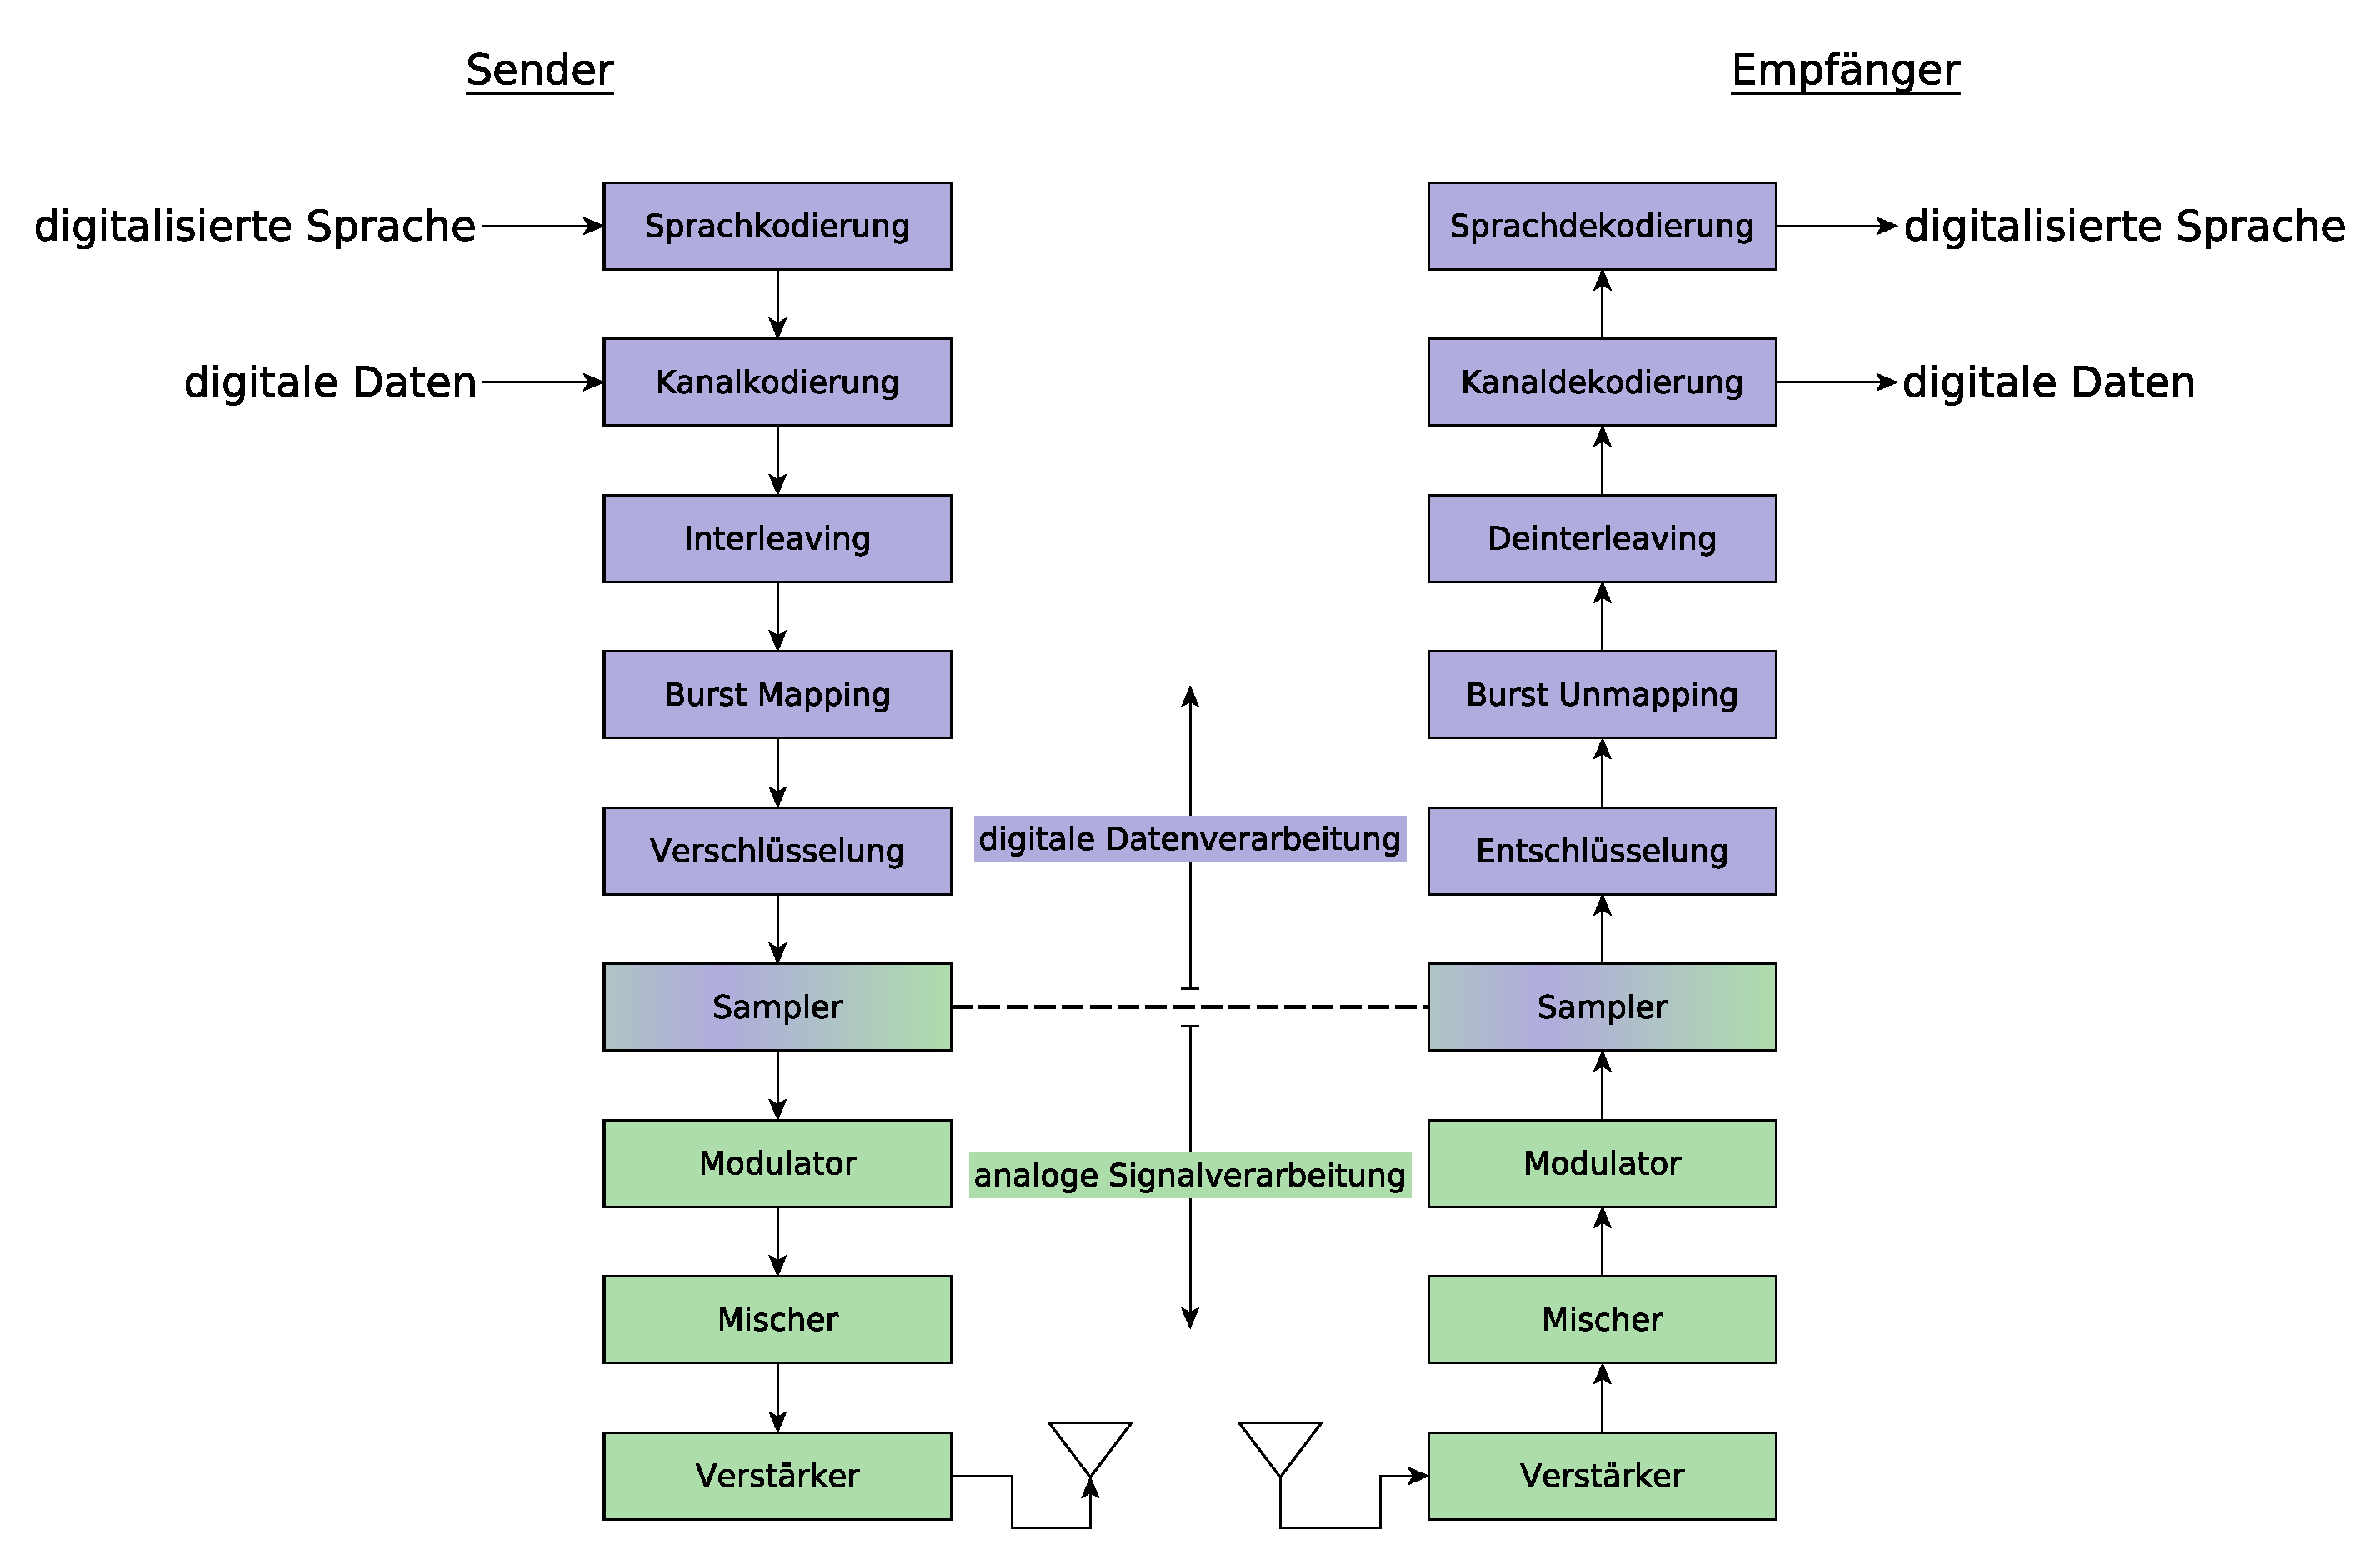
\includegraphics[width=1.0\textwidth]{figures/gsm_signal_processing.pdf}
  \end{center}
  \caption[Die Signalverarbeitung in GSM]{Die Signalverarbeitung in \ac{GSM}, erstellt mit yEd nach \citepauthor[Figure 1a]{3gpp:05.03} und \citep{zoudigital}} \label{fig:gsm-signal-processing} 
\end{figure}

Beim Sendevorgang laufen die diskreten, digitalen Daten nach Kanalkodierung und Verschlüsselung durch den Sampler, der sie in ein analoges Signal umwandelt. Dieses wird dann auf die bestehende Trägerfrequenz moduliert, gemischt und verstärkt übertragen. Beim Empfang der Daten werden die Schritte der digitalen und analogen Signalverarbeitung umgekehrt durchlaufen \citep{zoudigital}.

Aufgrund der hohen Anfälligkeit der Signalübertragung über die Luft werden Mechanismen zur Fehlererkennung und Korrektur angewandt, mit denen die Bitfehlerrate um den Faktor $10^{3}$ verringert werden kann \citep[Kap. 4.8]{eberspacher:2008:gsm-architecture}. Jeder logische Kanal hat andere Anforderungen an die übertragenen Daten. Deshalb werden, wie in \autoref{fig:0503fig1a-channel-coding} zu sehen, verschiedene Kodierungsverfahren kombiniert.

\begin{figure}[H]
  \begin{center}
    \includegraphics[width=0.9\textwidth]{figures/0503_fig_1a.pdf}
  \end{center}
  \caption[Die Kanalkodierung in GSM]{Die Kanalkodierung in \ac{GSM}, aus \citepauthor[Abb. 1a]{3gpp:05.03}} \label{fig:0503fig1a-channel-coding} 
\end{figure}

In \autoref{fig:0503fig1a-channel-coding} aus \citet{3gpp:05.03} sind die Kodierungsschritte aufgelistet, die für die verschiedenen logischen Kanäle durchlaufen werden. In jedem Kasten findet man unter dem Namen des Verfahrens die Nummer des Kapitels aus \citet{3gpp:05.03}, in dem es beschrieben wird. Die Call Setup Nachricht, die für den vorgestellten Angriff manipuliert werden muss, wird auf den Kanälen \ac{FACCH} oder \ac{SDCCH} übertragen. Die farblich markierten Verfahren sind also für die Arbeit besonders relevant und werden im Folgenden genauer erklärt.

\subsection{Blockcode}\label{hdl:blockcode}

Mit Blockcodes wird einem Block von Daten Redundanz für Fehlererkennung und/oder Fehlerkorrektur hinzugefügt. Der \ac{GSM}-Standard definiert den Einsatz von zwei Verfahren, \ac{CRC} für Nutzdatenkanäle und Firecode auf Signalisierungskanälen.

Auf Sprachkanälen werden die Informationsbits zudem in verschiedene Klassen eingeteilt, von denen nur Klasse 1 Bits besonders signifikant für die Spracherkennung sind und durch den \ac{CRC} fehlergeschützt werden. Klasse 2 Bits sind nicht so wichtig und fließen deshalb auch nicht in die Berechnung der Paritätsbits mit ein.

Für Signalisierungsnachrichten wird ein Firecode verwendet, ein linearer binärer Blockcode. Für eine Reihe von Informationsbits liefert dieser eine Anzahl redundanter Bits, die für die Fehlererkennung und -korrektur verwendet werden können. Die redundanten Bits werden durch \ac{XOR}, beziehungsweise binäre Addition der Informationsbits berechnet. 

Für alle zyklischen Codes kann die Berechnung der Redundanz als binäre Polynomdivision ausgedrückt werden. Aus der originalen Datensequenz wird ein Polynom aufgebaut, dessen Koeffizienten die Bits der Sequenz sind. Der Teiler ist ein definiertes Generatorpolynom und die Redundanz der Rest der Polynomdivision. Durch das Anhängen der Redundanz an die Datensequenz kann der Empfänger diese auf Fehler überprüfen, indem er ebenfalls durch das Generatorpolynom teilt. Ist das Ergebnis 0, sind keine Fehler aufgetreten. Es ist möglich, einen Sollrest anzugeben, der bei der Überprüfung der Datensequenz als Ergebnis herauskommen soll. Durch die \ac{XOR}-Verknüpfung der berechneten Redundanz mit dem Sollrest auf der Senderseite kommt dieser bei der Überprüfung durch den Empfänger wieder heraus. \ac{GSM} definiert als Sollrest die 40 Bits mit dem Wert 1, wodurch die Daten als fehlerfrei übertragen gelten, wenn das Ergebnis der Überprüfung \texttt{0xffffffffff} ist.
\begin{align}
&g: (x^{23} + 1) \cdot (x^{17} + x^3 + 1) = x^{40} + x^{26} + x^{23} + x^{17} + x^{3} + 1 \label{gl:firecode-gen}
\end{align}
Das Generatorpolynom (siehe \autoref{gl:firecode-gen}) des Firecodes und die Definition des Soll-Rests ist in \citetauthor[Kap. 4.1.2]{3gpp:05.03} zu finden.

Da die Eingangsdaten immer ein \ac{LAPDm} Frame sind, ist die Länge k der Informationsbits 184 Bit. Der Firecode generiert mit obigem Generatorpolynom, entsprechend dessen Grad, aus der 184 Bit langen Sequenz, 40 redundante Paritätsbits $p(k)$. In \ac{GSM} werden die berechneten Paritätsbits einfach an die Originaldaten $d(k)$ angehängt. Für die Weiterverarbeitung werden für die Faltungskodierung noch vier Nullbits angefügt, womit die ausgehenden Daten $u(k)$ die Länge von 228 Bit haben. Der Zusammenhang ist in  \autoref{eq:blockcode_2} mathematisch dargestellt.
\begin{align}\label{eq:blockcode_2}
\begin{split}
u(k) = d(k) &\quad \text{für} \, k= 0,1,...,183 \\
u(k) = p(k-184) &\quad \text{für} \, k = 184,185,...,223 \\
u(k) = 0 &\quad \text{für} \, k = 224,225,226,227
\end{split}
\end{align}
Das verwendete Generatorpolynom wurde von \citet{fire1959class} vorgestellt und bietet eine gute Erkennung und Korrektur von Fehlergruppen von bis zu 11 Bits. Obwohl eine Fehlerkorrektur möglich wäre, verzichtet \ac{GSM} darauf und verlässt sich stattdessen auf die erneute Übertragung der Nachricht, auf der von \ac{LAPDm} zur Verfügung gestellten, zuverlässigen Verbindung. In folgendem Beispiel wird der Firecode auf Testdaten angewendet.\\

%\begin{adjustbox}{max width={0.980\textwidth}, padding=3pt 2pt 3pt 0pt, frame, center}
\begin{lstlisting}[caption={[Kodierung von Testdaten mit dem Firecodes]Kodierung von Testdaten mit dem Firecodes, Datensatz generiert mit \texttt{dummycoder} (siehe \autoref{hdl:coder-impl})}, captionpos=b, language=bytetxt, numbers=none, frame=single]
Datensequenz (184 Bit):
01 20 51 03 45 04 04 60  02 00 81 5e 07 81 10 57 
81 81 81 81 15 01 01

Rest aus Polynomdivision mit Generatorpolynom (40 Bit): 
07 47 e3 10 1a

Soll-Rest in GSM (40 Bit):
ff ff ff ff ff

Paritätsbits in GSM == Rest XOR Soll-Rest (40 Bit):
f8 b8 1c ef e5

Anhängen von Paritäts- und Nullbits (228 Bit):
01 20 51 03 45 04 04 60  02 00 81 5e 07 81 10 57 
81 81 81 81 15 01 01 f8  b8 1c ef e5 0
\end{lstlisting}
%\end{adjustbox}

Blockcodes und zyklische Codes gehören zu den linearen Codes, weshalb Methoden der Linearen Algebra angewandt werden können. Für lineare Abbildungen gilt Additivität \citep[S. 142 ff.]{werner2008codierung}:
\begin{align}
\boldsymbol{u}(\boldsymbol{x} \oplus \boldsymbol{y}) = \boldsymbol{u}(\boldsymbol{x}) \oplus \boldsymbol{u}(\boldsymbol{y}) \label{gl:fire-lin}
\end{align}
Es können also die Paritätsbits berechnet werden, die bei einer Datenmanipulation kippen. Das bedeutet Blockcodes, wie der Firecode, sind nur für die Erkennung von zufälligen Fehlern ausgelegt und eignen sich nicht für den Schutz der Integrität.

\subsection{Faltungscode}\label{hdl:conv-code}

Durch Faltungskodierung, auch "`Convolutional Coding"' genannt, wird das Signal erneut mit Redundanz zur Fehlerkorrektur versehen. Wie Blockcodes lässt sich auch die Faltungskodierung polynomial beschreiben. Bei der Kodierung wird der Informationsgehalt der Eingangsbits, durch Faltung mit einer durch das Generatorpolynom definierten Maske, auf mehrere Ausgangsbits verteilt. Bei der Dekodierung kommt der Viterbi-Algorithmus zum Einsatz, der aus der kodierten Datensequenz die wahrscheinlichsten Ausgangsdaten bestimmt. Da beim Paritätscheck des Blockcodes die bereits durch den Viterbi-Dekodierer fehlerkorrigierten Daten eingehen, spricht man bei der Faltungskodierung von internem und beim Blockcode von externem Fehlerschutz \cite[Kap. 4.8.1, 4.8.2]{eberspacher:2008:gsm-architecture}.

Die Polynomdarstellung des in \ac{GSM} verwendeten "`$\nicefrac{1}{2}$ Rate Convolutional Coders"' ist in \citetauthor[Kap. 4.1.3]{3gpp:05.03} zu finden.
\begin{align}
\begin{split}
& g_0 = x^4 + x^3 + 1 \\
& g_1 = x^4 + x^3 + x + 1
\end{split}
\end{align}
Obige Gleichung bedeutet, das aus einem Eingangsbit $x$ zwei Bits $g_0$ und $g_1$ durch binäre Additionen von $x$ mit seinen Vorgängerbits generiert werden. Wo es keine Vorgängerbits gibt, werden diese als 0 definiert.

Die Eingangsdaten der Faltungskodierung sind die vom Blockcode generierte Datensequenzen. Das Ergebnis $c(k)$ der Faltungskodierung wird wie folgt als Funktion der Eingangsdaten $u(k)$ ausgedrückt:
\begin{align}\label{eq:convcode}
\begin{split}
& c(2k) = u(k-4) \oplus u(k-3) \oplus u(k) \\
& c(2k+1) = u(k-4) \oplus u(k-3) \oplus u(k-1) \oplus u(k) \quad \text{für} \, k = 0,1,...,227 \\
& u(j) = 0 \quad \forall \, j < 0
\end{split}
\end{align}\noindent
Die Faltungskodierung wird in Hardware als Schieberegister implementiert. Es wird ein Puffer von vier Bits benötigt, da die Bits bis zu vier Stellen vor dem Eingangsbit ($u(k-4)$) in die Berechnung mit eingehen. Der Puffer wird mit vier Speicherregistern realisiert. Durch die mit \ac{XOR}-Gattern implementierten Funktionen $c(2k)$ und $c(2k+1)$ werden zwei Ausgangsbits generiert. Welche Speicherregister verknüpft werden müssen, lässt sich aus \autoref{eq:convcode} ableiten. Da pro Eingangsbit zwei Ergebnisbits generiert werden, bezeichnet man den Kodierer als $\nicefrac{1}{2}$ Rate Convolutional Coder. Die vier nach dem Blockcode angehängten Nullbits sind notwendig, um das Schieberegister wieder in einen vordefinierten Zustand -- alle Register gleich 0 -- für den nächsten Block zu bringen.

\begin{figure}[H]
  \begin{center}
    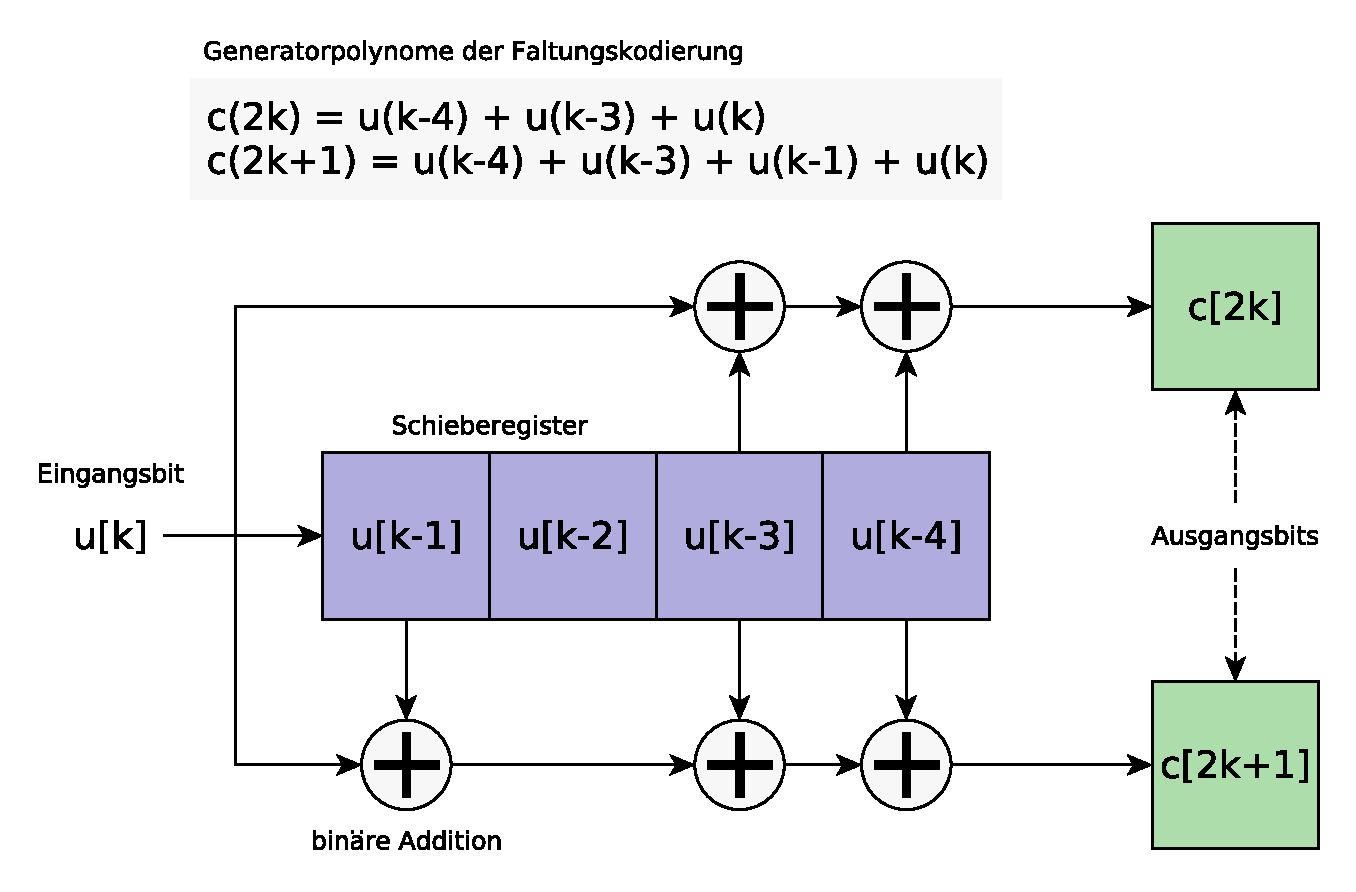
\includegraphics[width=1.0\textwidth]{figures/conv_code_shift_reg.pdf}
  \end{center}
  \caption[Das Schieberegister für die Faltungskodierung]{Das Schieberegister für die Faltungskodierung, erstellt mit yEd} \label{fig:conv_code_shift_reg} 
\end{figure}
Auf Signalisierungskanälen sind alle Datenbits wichtig und fließen in die Faltungskodierung mit ein. Bei Sprachkanälen hingegen wird ein sogenannter "`Punctured Convolutional Code"' verwendet. Um Bandbreite zu sparen werden dabei vom Kodierer nur die für die Wiederherstellung des Sprachsignals wichtigen Klasse 1 Bits kodiert, die unwichtigeren Klasse 2 Bits werden ohne Redundanz übertragen \citepauthor[Kap. 3.1.2, 3.2.2]{3gpp:05.03}. 

Wie Blockcodes gehört die Faltungskodierung zur Gruppe linearer Codes und es gilt Additivität \citep[S. 142 ff.]{werner2008codierung}:
\begin{align}
\boldsymbol{c}(\boldsymbol{x} \oplus \boldsymbol{y}) = \boldsymbol{c}(\boldsymbol{x}) \oplus \boldsymbol{c}(\boldsymbol{y})
\end{align}
In folgendem Beispiel wird die Faltungskodierung auf Testdaten angewendet.\\

%\begin{adjustbox}{max width={0.980\textwidth}, padding=3pt 2pt 3pt 0pt, frame, center}
\begin{lstlisting}[caption={[Faltungskodierung von Testdaten]Faltungskodierung von Testdaten, Datensatz generiert mit \texttt{dummycoder} (siehe \autoref{hdl:coder-impl})}, label=lst:conv_code_data, captionpos=b, language=bytetxt, numbers=none, frame=single]
Datensequenz (228 Bit):
01 20 51 03 45 04 04 60  02 00 81 5e 07 81 10 57 
81 81 81 81 15 01 01 f8  b8 1c ef e5 0

Faltungskodierte Daten (456 Bit): 
00 03 42 3c 37 bc 4f 0e  47 c7 bf 34 f0 34 c9 cc 
00 0d 3c 00 d3 c3 78 55  0c 3a 50 c3 4c 4f 37 85 
50 c3 9c c3 9c c3 9c c3  4c 78 bf 03 4f 03 a6 90 
1d 60 c3 a8 da e5 a9 3b  bf 
\end{lstlisting}
%\end{adjustbox}

\subsection{Interleaving}\label{hdl:interleaving}

Um gegen auf der Funkschnittstelle auftretende Burstfehler zu schützen, werden die Daten umsortiert und vom Interleaver verschachtelt. Blockweise Signalstörungen verteilen sich damit auf eine größere Datenmenge und können von der Fehlerkorrektur mit größerer Wahrscheinlichkeit berichtigt werden. Die aus dem Faltungskodierer kommenden Datenblöcke $N_n$ mit 456 kodierten und verschlüsselten Bits werden in Unterblöcke von je 57 Bits unterteilt. Je zwei solcher Unterblöcke werden einem Burst $B_b$ zugewiesen (siehe \autoref{fig:normal_burst}). Für Sprachkanäle wird die Stelle im Burst $B_b[j]$, an dem ein Bit eines Datenblocks $N_n[k]$ landet, in \citetauthor[Kap. 3.1.3]{3gpp:05.03} wie folgt bestimmt:
\begin{align}
\begin{split}
& i(B_b,j) = c(N_n,k) \\
& k = 0,1,...,455 \\
& n = 0,1,... \\
& b = 4 \cdot n + \left(k \bmod 8\right) \\
& j = 2 \cdot \left(\left( 49 \cdot k \right) \bmod 57 \right) + \left(\left( k \bmod 8 \right) \bdiv 4 \right)
\end{split}
\end{align}
Die Nummer des Bursts wird also durch die Nummer des Datenblocks und den Laufindex $k$ modulo $8$ auf diesem bestimmt. Das heißt jedes der acht Bits eines Bytes wird in einem anderen Burst untergebracht. Wird ein kompletter Burst fehlerhaft übertragen, erhält man auf Empfängerseite nach dem Deinterleaving die 114 fehlerhaften Bits auf einen Fehler pro Byte verteilt. So verteilte Bitfehler können von der Fehlerkorrektur berichtigt werden.

In \citetauthor[Tabelle 1]{3gpp:05.03} ist das Ergebnis von Interleaving und Umsortierung der Bits aufgelistet. Die Daten eines Blockes $N_n$ sind so auf die Bursts verteilt, dass die vorderen vier Bursts $B_{4n + 0,1,2,3}$ immer die geraden Bits [0-56] und die hinteren vier Burst $B_{4n + 4,5,6,7}$ die ungeraden Bits [57-113] enthalten. Das bedeutet, dass ein Burst immer die Daten von zwei Datenblöcken $N_n$ und $N_{n + 1}$ enthält. Die geraden Datenbits stammen aus dem höheren, die ungeraden aus dem niedrigeren Block. Diese Art der Verzahnung nennt man block-diagonales Interleaving. Alle vier Bursts beginnt ein neuer Datenblock, der in acht Bursts komplett übertragen wird. Die Übertragung einer gesamten Sprachprobe dauert somit $8 \cdot 4.615 ms = 30 ms$. Folgendes Beispiel zeigt das Ergebnis von block-diagonalem Interleaving, angewendet auf das das Ergebnis der Faltungskodierung aus \autoref{lst:conv_code_data}. Die Daten werden binär dargestellt und sind bereits ihren Bursts zugewiesen, zur besseren Kenntlichkeit sind binäre Einsen rot und Nullen blau markiert. Im Beispiel ist nur das Ergebnis des Interleaving für den Datenblock $N_n$ dargestellt, nicht die Überlagerung mit vorherigem und nachfolgenden Datenblock. So kann man erkennen, dass Bit [57-113] der ersten vier Bursts und Bit [0-56] der zweiten vier Bursts nicht befüllt sind (alle Bits gleich Null). Bit [57-113] der ersten vier Bursts wäre vom Datenblock $N_{n-1}$ befüllt worden, $N_{n+1}$ würde Bit [0-56] der zweiten vier Bursts befüllen.\\

\begin{samepage}
\begin{adjustbox}{max width={0.995\textwidth}, padding=4pt 2pt 4pt 0pt, frame, center}
\begin{lstlisting}[language=bytetxt, numbers=none]
Bit[0-56]                                                 Bit[57-113]
!!00000000000000!!@1@!!000!!@1@!!000!!@1@!!0!!@1@!!0!!@1@!!00000!!@1@!!00000!!@1@!!0!!@1@!!0!!@1@!!0!!@1@!!000!!@1@!!000!!@1@!!000!!@1@ !!000000000000000000000000000000000000000000000000000000000!! Burst 0
!!00!!@1@!!0!!@1@!!000!!@1@!!00000!!@1@!!0!!@1@!!0!!@1@!!0000000000000!!@1@!!0!!@1@!!0!!@1@!!000!!@1@!!000!!@1@!!0!!@1@!!0!!@1@!!000!!@1@!!0!!@1@!!00!! !!000000000000000000000000000000000000000000000000000000000!! Burst 1
!!00!!@1@!!0!!@1@!!000!!@1@!!0!!@1@!!0!!@1@!!0!!@1@!!000000000!!@1@!!0!!@1@!!0!!@1@!!00000000000!!@1@!!0!!@1@!!000000000!!@1@!!000!!@1@ !!000000000000000000000000000000000000000000000000000000000!! Burst 2
!!0000000000!!@1@!!0!!@1@!!0!!@1@!!000!!@1@!!000!!@1@!!0!!@1@!!0!!@1@!!0000000000000!!@1@!!0!!@1@!!0!!@1@!!0!!@1@!!0!!@1@!!00000000!! !!000000000000000000000000000000000000000000000000000000000!! Burst 3
!!000000000000000000000000000000000000000000000000000000000!! @1@!!000!!@1@!!0!!@1@!!0!!@1@!!0!!@1@!!0!!@1@!!000000000!!@1@!!0!!@1@!!0!!@1@!!0!!@1@!!000!!@1@!!000!!@1@!!0!!@1@!!00000!!@1@!!000000000000!! Burst 4
!!000000000000000000000000000000000000000000000000000000000!! @1@!!0000000!!@1@!!00000!!@1@!!0!!@1@!!0!!@1@!!000!!@1@!!0!!@1@!!000!!@1@!!00000!!@1@!!0!!@1@!!00000!!@1@!!0!!@1@!!0!!@1@!!000!!@1@!!0!!@1@!!0000!! Burst 5
!!000000000000000000000000000000000000000000000000000000000!! !!00!!@1@!!0000000!!@1@!!0!!@1@!!0!!@1@!!0!!@1@!!000!!@1@!!000!!@1@!!00000!!@1@!!0!!@1@!!0000000!!@1@!!0!!@1@!!0!!@1@!!000!!@1@!!0!!@1@!!000000!! Burst 6
!!000000000000000000000000000000000000000000000000000000000!! @1@!!0!!@1@!!0!!@1@!!000!!@1@!!00000!!@1@!!000000000!!@1@!!0!!@1@!!0!!@1@!!00000!!@1@!!0000000!!@1@!!0!!@1@!!0!!@1@!!0!!@1@!!0!!@1@!!000!!@1@!!00!! Burst 7
\end{lstlisting}
\end{adjustbox}
\begin{lstlisting}[caption={[Verschachtlung von Testdaten mit block-diagonalem Interleaving]Verschachtlung von Testdaten mit block-diagonalem Interleaving, Datensatz generiert mit \texttt{dummycoder} (siehe \autoref{hdl:coder-impl})}, basicstyle=\tiny, label=lst:interl-block-diag]
\end{lstlisting}
\end{samepage}

Das für Signalisierungskanäle angewandte Interleaving \citepauthor[Kap. 4.1.4]{3gpp:05.03} unterscheidet sich nur in der Verteilung der 57 Bit Blöcke auf die Bursts.
\begin{align}
\begin{split}
& i(B_b,j) = c(N_n,k) \\
& k = 0,1,...,455 \\
& n = 0,1,... \\
& b = 4 \cdot n + \left(k \bmod 4\right) \\
& j = 2 \cdot \left(\left( 49 \cdot k \right) \bmod 57 \right) + \left(\left( k \bmod 8 \right) \bdiv 4 \right)
\end{split}
\end{align}
Im Gegensatz zum block-diagonalen Interleaving werden die generierten Blöcke auf nur vier Bursts aufgeteilt. Es gibt keine Verzahnung von aufeinander folgenden Datenblöcken, wodurch eine Signalisierungsnachricht nach $4 \cdot 4.615 ms = 15 ms$ komplett übertragen ist. Ein Burst $B_{4n + 1,2,3,4}$ enthält also eine Kombination von geraden und ungeraden Daten des selben Datenblocks $N_n$. Das Verfahren wird deshalb block-rectangular Interleaving genannt. Die Verteilung der Bits eines Datenblocks $N_n$ auf die Burst mit block-rectangular Interleaving, ist in folgendem Beispiel dargestellt. Es werden die selbigen Eingangsdaten verwendet wie in \autoref{lst:interl-block-diag}. Anschaulich gesagt wandern Bit [57-113] der zweiten vier Bursts "`nach oben"', in die ersten vier Bursts.\\

\begin{samepage}
\begin{adjustbox}{max width={0.995\textwidth}, padding=4pt 2pt 4pt 0pt, frame, center}
\begin{lstlisting}[language=bytetxt, numbers=none]
Bit[0-56]                                                 Bit[57-113]
!!00000000000000!!@1@!!000!!@1@!!000!!@1@!!0!!@1@!!0!!@1@!!00000!!@1@!!00000!!@1@!!0!!@1@!!0!!@1@!!0!!@1@!!000!!@1@!!000!!@1@!!000!!@1@ @1@!!000!!@1@!!0!!@1@!!0!!@1@!!0!!@1@!!0!!@1@!!000000000!!@1@!!0!!@1@!!0!!@1@!!0!!@1@!!000!!@1@!!000!!@1@!!0!!@1@!!00000!!@1@!!000000000000!! Burst 0
!!00!!@1@!!0!!@1@!!000!!@1@!!00000!!@1@!!0!!@1@!!0!!@1@!!0000000000000!!@1@!!0!!@1@!!0!!@1@!!000!!@1@!!000!!@1@!!0!!@1@!!0!!@1@!!000!!@1@!!0!!@1@!!00!! @1@!!0000000!!@1@!!00000!!@1@!!0!!@1@!!0!!@1@!!000!!@1@!!0!!@1@!!000!!@1@!!00000!!@1@!!0!!@1@!!00000!!@1@!!0!!@1@!!0!!@1@!!000!!@1@!!0!!@1@!!0000!! Burst 1
!!00!!@1@!!0!!@1@!!000!!@1@!!0!!@1@!!0!!@1@!!0!!@1@!!000000000!!@1@!!0!!@1@!!0!!@1@!!00000000000!!@1@!!0!!@1@!!000000000!!@1@!!000!!@1@ !!00!!@1@!!0000000!!@1@!!0!!@1@!!0!!@1@!!0!!@1@!!000!!@1@!!000!!@1@!!00000!!@1@!!0!!@1@!!0000000!!@1@!!0!!@1@!!0!!@1@!!000!!@1@!!0!!@1@!!000000!! Burst 2
!!0000000000!!@1@!!0!!@1@!!0!!@1@!!000!!@1@!!000!!@1@!!0!!@1@!!0!!@1@!!0000000000000!!@1@!!0!!@1@!!0!!@1@!!0!!@1@!!0!!@1@!!00000000!! @1@!!0!!@1@!!0!!@1@!!000!!@1@!!00000!!@1@!!000000000!!@1@!!0!!@1@!!0!!@1@!!00000!!@1@!!0000000!!@1@!!0!!@1@!!0!!@1@!!0!!@1@!!0!!@1@!!000!!@1@!!00!! Burst 3
\end{lstlisting}
\end{adjustbox}
\begin{lstlisting}[caption={[Verschachtlung von Testdaten mit block-rectangular Interleaving]Verschachtlung von Testdaten mit block-rectangular Interleaving, Datensatz generiert mit \texttt{dummycoder} (siehe \autoref{hdl:coder-impl})}, basicstyle=\tiny]
\end{lstlisting}
\end{samepage}

\subsection{Burst Mapping}\label{hdl:burst-mapping}
Ein normaler Burst enthält zusätzlich zu den zwei 57 Bit Blöcken an Daten noch sogenannte "`Stealing Flags"' (siehe \autoref{fig:normal_burst}). Sie sind gesetzt, wenn die Daten des ihnen zugeordneten 57 Bit Blockes für die Übertragung von Signalisierungsinformationen genutzt werden. Auf Sprachkanälen kann der \ac{FACCH} somit die Bandbreite des \ac{TCH} mitbenutzen. Die Sprachdaten auf dem \ac{TCH}, die so durch Signalisierungsdaten des \ac{FACCH} ersetzt werden, werden verworfen \citepauthor[Kap. 4.3.5]{3gpp:05.03}. Der \ac{FACCH} stiehlt also Bandbreite vom \ac{TCH}, was den Namen des Flags erklärt. Auf Kanälen wie dem \ac{SDCCH}, die nur Signalisierungsinformationen übertragen, sind immer beide Flags gesetzt \citepauthor[Kap. 4.5, 4.1.5]{3gpp:05.03}.

"`Burst Mapping"' fügt in die vom Interleaving erstellten 57 Bit Blöcke Stealing Flags ein und ordnet jeweils zwei der entstandenen 58 Bit Blöcke den 116 Bit Nutzdaten eines fertigen Bursts zu. Das Beispiel zeigt die Zuordnung der schon in \autoref{hdl:interleaving} verwendeten, auf einem \ac{SDCCH} übertragenen Signalisierungsnachricht. In diesem Fall werden beide Stealing Flags gesetzt. Würde die Signalisierungsnachricht auf einem \ac{FACCH} übertragen werden, wäre sie vom Burstmapping auf acht Bursts verteilt worden. Jedem der acht Bursts würde dann nur die Hälfte seiner Nutzdaten gestohlen werden.\\

\begin{samepage}
\begin{adjustbox}{max width={0.995\textwidth}, padding=4pt 2pt 4pt 0pt, frame, center}
\begin{lstlisting}[language=bytetxt, numbers=none]
Bit[0-56]                                                     Bit[59-115]
!!00000000000000!!@1@!!000!!@1@!!000!!@1@!!0!!@1@!!0!!@1@!!00000!!@1@!!00000!!@1@!!0!!@1@!!0!!@1@!!0!!@1@!!000!!@1@!!000!!@1@!!000!!@1@ @1@ @1@ @1@!!000!!@1@!!0!!@1@!!0!!@1@!!0!!@1@!!0!!@1@!!000000000!!@1@!!0!!@1@!!0!!@1@!!0!!@1@!!000!!@1@!!000!!@1@!!0!!@1@!!00000!!@1@!!000000000000!! Burst 0
!!00!!@1@!!0!!@1@!!000!!@1@!!00000!!@1@!!0!!@1@!!0!!@1@!!0000000000000!!@1@!!0!!@1@!!0!!@1@!!000!!@1@!!000!!@1@!!0!!@1@!!0!!@1@!!000!!@1@!!0!!@1@!!00!! @1@ @1@ @1@!!0000000!!@1@!!00000!!@1@!!0!!@1@!!0!!@1@!!000!!@1@!!0!!@1@!!000!!@1@!!00000!!@1@!!0!!@1@!!00000!!@1@!!0!!@1@!!0!!@1@!!000!!@1@!!0!!@1@!!0000!! Burst 1
!!00!!@1@!!0!!@1@!!000!!@1@!!0!!@1@!!0!!@1@!!0!!@1@!!000000000!!@1@!!0!!@1@!!0!!@1@!!00000000000!!@1@!!0!!@1@!!000000000!!@1@!!000!!@1@ @1@ @1@ !!00!!@1@!!0000000!!@1@!!0!!@1@!!0!!@1@!!0!!@1@!!000!!@1@!!000!!@1@!!00000!!@1@!!0!!@1@!!0000000!!@1@!!0!!@1@!!0!!@1@!!000!!@1@!!0!!@1@!!000000!! Burst 2
!!0000000000!!@1@!!0!!@1@!!0!!@1@!!000!!@1@!!000!!@1@!!0!!@1@!!0!!@1@!!0000000000000!!@1@!!0!!@1@!!0!!@1@!!0!!@1@!!0!!@1@!!00000000!! @1@ @1@ @1@!!0!!@1@!!0!!@1@!!000!!@1@!!00000!!@1@!!000000000!!@1@!!0!!@1@!!0!!@1@!!00000!!@1@!!0000000!!@1@!!0!!@1@!!0!!@1@!!0!!@1@!!0!!@1@!!000!!@1@!!00!! Burst 3
                                                          ^ ^
                Stealing Bit [57] für Daten von Bit[0-56]  |  Stealing Bit [58] für Daten von Bit[59-115]                                                           
                                       <-----------------  |  -----------------> 
\end{lstlisting}
\end{adjustbox}
\begin{lstlisting}[caption={[Zuordnung von Testdaten zu Bursts auf dem SDCCH durch Burstmapping]Zuordnung von Testdaten zu Bursts auf dem \ac{SDCCH} durch Burstmapping, Datensatz generiert mit \texttt{dummycoder} (siehe \autoref{hdl:coder-impl})}, basicstyle=\tiny]
\end{lstlisting}
\end{samepage}

\section{Sicherheit in GSM} \label{hdl:sicherheitsmechanismen-gsm_authentifizierung}

\acused{A3}
\acused{A8}
\acused{A5}
\acused{SRES}
\acused{Ki}
\acused{RES}
\acused{RAND}
\acused{COMP128}

Da auf der Funkschnittstelle jeder Mithören kann, der ein entsprechendes Empfangsgerät besitzt, spezifiziert \ac{GSM} verschiedene Techniken und Funktionen, um den Schutz, sowie die Authentizität der Identitäten der Netzteilnehmer und die Vertraulichkeit der kommunizierten Daten zu gewährleisten. 

Die Teilnehmeridentität wird durch Verwendung einer \ac{TMSI} zur Identifikation des \ac{MS} beim Netzwerk geschützt. Ein Teilnehmer erhält vom Netzwerk diese temporäre Identifikationsnummer, die er statt seiner eindeutigen \ac{IMSI} benutzen kann, um sich für die Nutzung von Diensten beim Netzwerk zu identifizieren \citepauthor{3gpp:03.20}.

Um Authentizität von Teilnehmeridentitäten und die Vertraulichkeit von kommunizierten Nutzdaten und Signalisierungsinformationen sicherzustellen, werden in \citetauthor{3gpp:03.20} die Algorithmen \ac{A3}, \ac{A8} und \ac{A5} definiert. Eine Beschreibung der Algorithmen findet sich nicht im Standard, die Algorithmen konnten aber durch Reverse Enginnering herausgefunden werden. So veröffentlichten \citet{briceno1998implementation} die Implementierung von \ac{COMP128}, einer Kombination der \ac{A3} und \ac{A8} Algorithmen und \citet{briceno1999pedagogical} die Implementierung von A5/1 und A5/2. Mit der Entwicklung neuerer Algorithmen hat \ac{3GPP} den "`Security by Obscurity"' Ansatz fallen gelassen. So steht zum Beispiel die Spezifikation von A5/3 auf der Website von \ac{3GPP} zu Verfügung\footnote{\url{http://www.3gpp.org/specifications/60-confidentiality-algorithms}}. Die Implementierung von \ac{A3} und \ac{A8} wurde von \ac{3GPP} als netzanbieterspezifisch bezeichnet, \ac{COMP128} wäre nur eine Beispielimplementierung gewesen und war nicht für den konkreten Einsatz gedacht. A5/1 und A5/2 wurden von \ac{3GPP} auch nachträglich nicht mehr selbst veröffentlicht, finden sich aber online\footnote{\url{http://www.scard.org/gsm/}}. Die folgenden Abschnitte gehen näher auf die in \ac{GSM} verwendeten Sicherheitsalgorithmen ein.

\subsection{GSM Authentifizierung} \label{hdl:authentication}

\begin{figure}[H]
  \begin{center}
    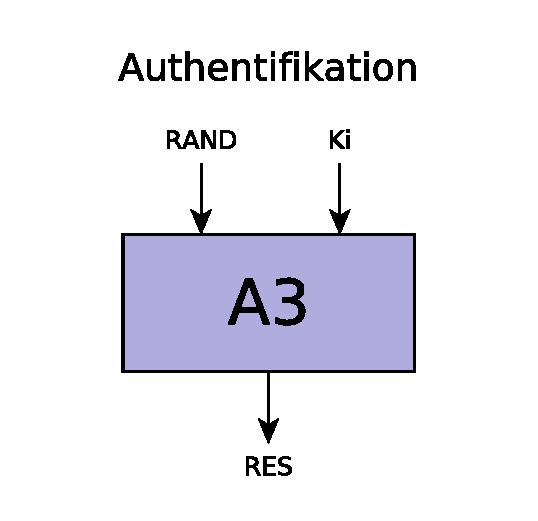
\includegraphics[width=0.5\textwidth]{figures/gsm_a3.pdf}
  \end{center}
  \caption[Der A3-Algorithmus]{Der \ac{A3}-Algorithmus, erstellt mit yEd nach \citepauthor[Abb. 3.1]{3gpp:03.20}} \label{fig:a3-algorithm}
\end{figure}

Die Authentifizierung wird vom Netzwerk gestartet. Zuerst werden vom \ac{MSC} die für die Überprüfung der Identität des Teilnehmers benötigten Werte mit seiner \ac{IMSI} beim \ac{AuC} angefragt. Das \ac{AuC} generiert die zufällige Challenge \ac{RAND} und holt sich vom \ac{HLR} den geheimen Schlüssel \ac{Ki} für die erhaltene \ac{IMSI}. Aus den beiden wird mit dem Authentifizierungsalgorithmus \ac{A8} die erwartete Antwort \ac{SRES} des Teilnehmers berechnet \citepauthor[Kap. 3, Anhang C.2]{3gpp:03.20}. Die berechneten Werte werden konkateniert und als Authentifizierungsvektor [$\ac{RAND}\parallel\ac{SRES}$] an das \ac{MSC} zurückgeschickt. Das \ac{MSC} kann der \ac{MS} nun den Authentication-Request mit der vom Netzwerk benutzten Challenge \ac{RAND} schicken. Erhält die \ac{MS} einen Authentication-Request, lässt es von der \ac{SIM}-Karte, die Zugriff auf \ac{A8} und \ac{Ki} hat, das Ergebnis \ac{RES} berechnen. Die Anfrage vom \ac{MSC} wird dann mit einer Authentication-Response, die \ac{RES} enthält, beantwortet. Ist der Vergleich $\ac{RES} == \ac{SRES}$ im \ac{MSC} erfolgreich, so ist die \ac{MS} authentifiziert.

Da das Verfahren keine gegenseitige Authentifizierung zulässt, sondern nur die des Netzteilnehmers, ermöglicht es einem Angreifer eine falschen \ac{BTS} zu installieren, dessen Identität von der \ac{MS} nicht überprüft werden kann. Durch die Einführung von gegenseitiger Authentifizierung mit dem \ac{UMTS}-\ac{AKA} und der Möglichkeit, dieses auch in \ac{GSM}-Netzwerken zu verwenden, wurde diese Schwachstelle behoben. Das Verfahren und die mögliche Interoperabilität mit 2G Infrastruktur wird in \autoref{hdl:umts-aka} erklärt.

\subsection{GSM Schlüsselgenerierung} \label{hdl:keygen}

\begin{figure}[H]
  \begin{center}
    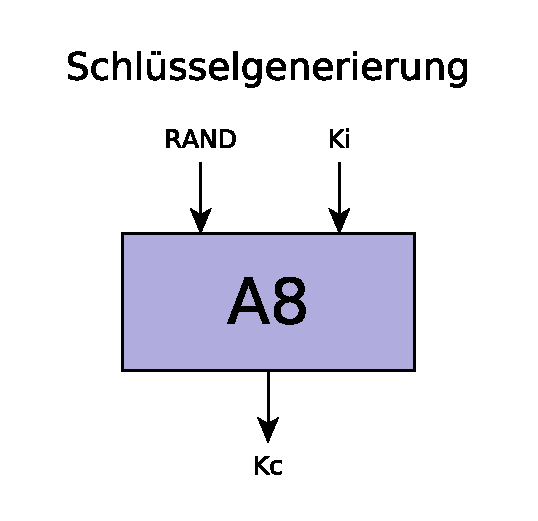
\includegraphics[width=0.5\textwidth]{figures/gsm_a8.pdf}
  \end{center}
  \caption[Der A8-Algorithmus]{Der \ac{A8}-Algorithmus, erstellt mit yEd nach \citepauthor[Abb. 4.1]{3gpp:03.20}} \label{fig:a8-algorithm}
\end{figure}

Nach erfolgreicher Authentifikation des Netzteilnehmers wird, mit dem Algorithmus \ac{A8} zur Schlüsselgenerierung, auf beiden Seiten ein 64 Bit langer \ac{Kc} berechnet, der für die weitere Verschlüsselung dieser Verbindung verwendet wird \citepauthor[Kap. 4.3, Anhang C.3]{3gpp:03.20}. Die Eingangsparameter von \ac{A8} sind die gleichen wie von \ac{A3}, vermutlich ein Grund für deren gemeinsame Implementierung in \ac{COMP128}.

Die Kombination der Verfahren zur Authentifizierung und Schlüsselgenerierung in \ac{GSM} wird \ac{AKA} genannt. Nach der Schlüsselgenerierung wird \ac{Kc} in \ac{MS} und \ac{BTS} als sogenannter Security Context unter einer \ac{CKSN} abgespeichert. Da die \ac{CKSN} bereits beim CM Service Request mitgeschickt wird, kann die \ac{BTS} prüfen, ob bereits ein gültiger Security Context mit der \ac{MS} besteht und diesen wiederverwenden. Das \ac{AKA} muss also nicht erneut ausgeführt werden, da der kryptografische Schlüssel \ac{Kc} beiden Seiten bereits bekannt ist. 

\subsection{UMTS Authentication and Key Agreement} \label{hdl:umts-aka}

\acused{K}
\acused{XMAC} 

Für \ac{UMTS} wurde mit dem 3G \ac{AKA} ein gegenseitiges Authentifizierungsverfahren spezifiziert \citepauthor{3gpp:33.102}, um die Schwachstellen der nur einseitigen 2G Authentifizierung zu beheben. Dadurch wird es einem Angreifer erschwert, in einem 3G Netzwerk eine falsche \ac{BTS} auf der \ac{Um}-Schnittstelle zu installieren, da die Authentizität des Netzwerks vom Netzteilnehmer überprüft werden kann. Außerdem wurde die Länge des zwischen 3G \ac{AuC} und \ac{USIM} geteilten geheimen Schlüssels \ac{K} von den in \ac{GSM} verwendeten 64 Bit auf 128 Bit erhöht. \autoref{fig:umts-auth-vec} zeigt die in den \ac{AUTN} einfließenden Werte und \autoref{fig:umts-auth-vec} wie die Authentifizierung des Netzwerks in der \ac{USIM} abläuft. Im \ac{UMTS}-Standard haben sich einige Bezeichnungen verändert, so wird \ac{MS} zu \ac{ME}, \ac{Ki} zu \ac{K}, und \ac{SRES} zu \ac{XRES}.

\begin{figure}[H]
  \begin{center}
    \includegraphics[width=0.7\textwidth]{figures/33102_fig_7}
  \end{center}
  \caption[Die Generierung des UMTS Authentifizierungsvektors]{Die Generierung des \ac{UMTS} Authentifizierungsvektors, aus \citepauthor[Abb. 7]{3gpp:33.102}} \label{fig:umts-auth-vec}
\end{figure}

Wie in \ac{GSM} erzeugt das \ac{AuC} zuerst eine zufällige Challenge \ac{RAND} und eine teilnehmerspezifische \ac{SQN} \citepauthor[Anhang C.1 und C.2]{3gpp:33.102}. Diese Sequenznummer bietet Schutz vor Replay-Attacken mit aufgezeichneten Authentifizierungsabläufen, da das \ac{ME} nur Anfragen akzeptiert, deren \ac{SQN} ungefähr gleich der im \ac{ME} mitgezählten \ac{SQN} ist. Ein proprietäres \ac{AMF} geht ebenfalls in die Berechnung mit ein \citepauthor[Anhang H]{3gpp:33.102}.
Das \ac{AuC} erzeugt dann folgende Werte:
\begin{itemize}
\item \textbf{\acf{MAC}}: $MAC = f1_K (SQN \parallel RAND \parallel AMF)$ 
\item \textbf{\acf{XRES}}: $XRES = f2_K (RAND)$ wobei f1 und f2 Authentifizierungsfunktionen sind.
\item \textbf{\acf{CK}}: $CK = f3_K (RAND)$
\item \textbf{\acf{IK}}: $IK = f4_K (RAND)$
\item \textbf{\acf{AK}}: $AK = f5_K (RAND)$ wobei f3, f4 und f5 Schlüsselerzeugungsfunktionen sind. \ac{AK} wird benutzt um die Sequenznummer zu anonymisieren und kann auch 0 sein, wenn das nicht erforderlich ist.
\end{itemize}
Aus diesen wird schließlich der Authentifizierungsvektor $\ac{AUTN} = \ac{SQN} \oplus \ac{AK} \parallel \ac{AMF} \parallel \ac{MAC}$ gebildet und im Authentication-Request an den Mobilfunkteilnehmer ausgeliefert.

\begin{figure}[H]
  \begin{center}
    \includegraphics[width=0.7\textwidth]{figures/33102_fig_9}
  \end{center}
  \caption[Die Authentifizierung des Netzwerks in der USIM]{Die Authentifizierung des Netzwerks in der \ac{USIM}, aus \citepauthor[Abb. 9]{3gpp:33.102}} \label{fig:auth-in-usim}
\end{figure}

Erhält das \ac{ME} den Authentication-Request des Netzwerks, so kann es mit der \ac{AUTN} überprüfen, ob dieses Kenntnis seines geheimen Schlüssels \ac{K} hat. 

Als erstes löst es die Anonymisierung der Sequenznummer auf und holt sich deren Wert mit $\ac{SQN} = (\ac{SQN} \oplus \ac{AK}) \oplus \ac{AK}$, wobei für die Berechnung von \ac{AK} die Funktion f5, die auch dem \ac{AuC} zur Verfügung steht, benutzt wird. Sollte die erhaltene \ac{SQN} nicht innerhalb der richtigen Größenordnung liegen, wird ein Synchronisationsfehler mit der aktuellen \ac{SQN} der \ac{USIM} an das Netzwerk zurückgeschickt und die laufende Authentifizierung abgebrochen.

Mit der Sequenznummer und \ac{AMF} kann nun aus dem \ac{AUTN} der erwartete Authentifizierungscode des Netzwerks \ac{XMAC} berechnet werden. Wenn dieser gleich dem aus \ac{AUTN} erhaltenen \ac{MAC} ist, weiß die \ac{USIM}, dass das Netzwerk ebenfalls den geheimen Schlüssel \ac{K} kennt. Das Netzwerk ist somit authentifiziert und die Authentication-Response mit dem Ergebnis \ac{RES} wird zurückgeschickt. Die anschließende Authentifizierung der Netzteilnehmer läuft wie in \ac{GSM} durch die Überprüfung \ac{RES} == \ac{XRES} des Netzwerks.

Der Schlüssel \ac{CK} geht dann in den Verschlüsselungsalgorithmus ein und sorgt wie schon in \ac{GSM}, für Vertraulichkeit der Daten. \ac{IK} ist in 3G neu und wird verwendet, um mit der Integritätsfunktion f9 \citepauthor[Kap. 6.5.3]{3gpp:33.102} die Integrität der Daten sicherzustellen.

Das für \ac{UMTS} spezifizierte \ac{AKA} kann in \ac{GSM} ebenfalls benutzt werden, sofern der Netzteilnehmer und das \ac{AuC} die 3G Authentifizierungsverfahren unterstützen. \autoref{fig:3g-aka-in-2g} zeigt die verschiedenen Möglichkeiten der Interoperabilität zwischen 2G und 3G Netzwerk- und \ac{ME}. Da aktuelle \acp{ME} (Mobilfunkgeräte, \ac{USIM}) und Kernnetzwerke (\ac{AuC}) alle 3G kompatibel sind, wird das \ac{GSM}-\ac{AKA} in der Regel nicht mehr benutzt.

\begin{figure}[H]
  \begin{center}
    \includegraphics[width=0.8\textwidth]{figures/31900_fig_1}
  \end{center}
  \caption[Interoperabilität des 3G AKA mit 2G Netzwerken]{Interoperabilität des 3G \ac{AKA} mit 2G Netzwerken, aus \citepauthor[Abb. 1]{3gpp:31.900}} \label{fig:3g-aka-in-2g}
\end{figure}

Die Verwendung des \ac{UMTS}-AKA in 2G Netzwerken basiert darauf, dass das \ac{MSC} den vom \ac{AuC} erhaltenen Wert (\ac{RAND} oder \ac{AUTN}) einfach nur in den Authentication-Request einfügt und weiterleitet und \ac{SRES} nicht selbst berechnet. Von einem 3G-fähigen \ac{AuC} erhält die \ac{USIM} also den Wert von \ac{AUTN}, mit dem sie das Netzwerk authentifizieren kann. Für die Authentication-Response muss die \ac{USIM} die korrekte Antwort \ac{RES} berechnen mit der sie, wie im 2G Standard definiert, im \ac{MSC} authentifiziert wird. Die einzigen Komponenten, die für die Ausführung des \ac{UMTS}-\ac{AKA} 3G-fähig sein müssen, sind also \ac{USIM} und \ac{AuC}. Der von f3 berechnete kryptografische Schlüssel \ac{CK} wird von der 2G \ac{BTS} als \ac{Kc} verwendet. Für den Integritätsschlüssel \ac{IK} hat die \ac{BTS} aber keine Verwendung. Die Integrität der übertragenen Daten bleibt weiterhin ungeschützt.

\subsection{Verschlüsselung} \label{hdl:ciphering}

Bevor die Kommunikation über die Funkschnittstelle verschlüsselt werden kann, muss der verwendete \ac{A5}-Algorithmus zwischen \ac{MS} und \ac{BTS} ausgehandelt werden \citepauthor[Kap. 4.8]{3gpp:03.20}, was in der "`\ac{MM} Connection Establishment Prozedur"' \citepauthor[Kap. 4.5.1.1]{3gpp:24.008} genau beschrieben wird. Die \ac{A5}-Algorithmen sind in der Hardware von Endgerät und \ac{BTS} realisiert, da sie in Echtzeit verschlüsseln und entschlüsseln müssen.

\begin{figure}[H]
  \begin{center}
    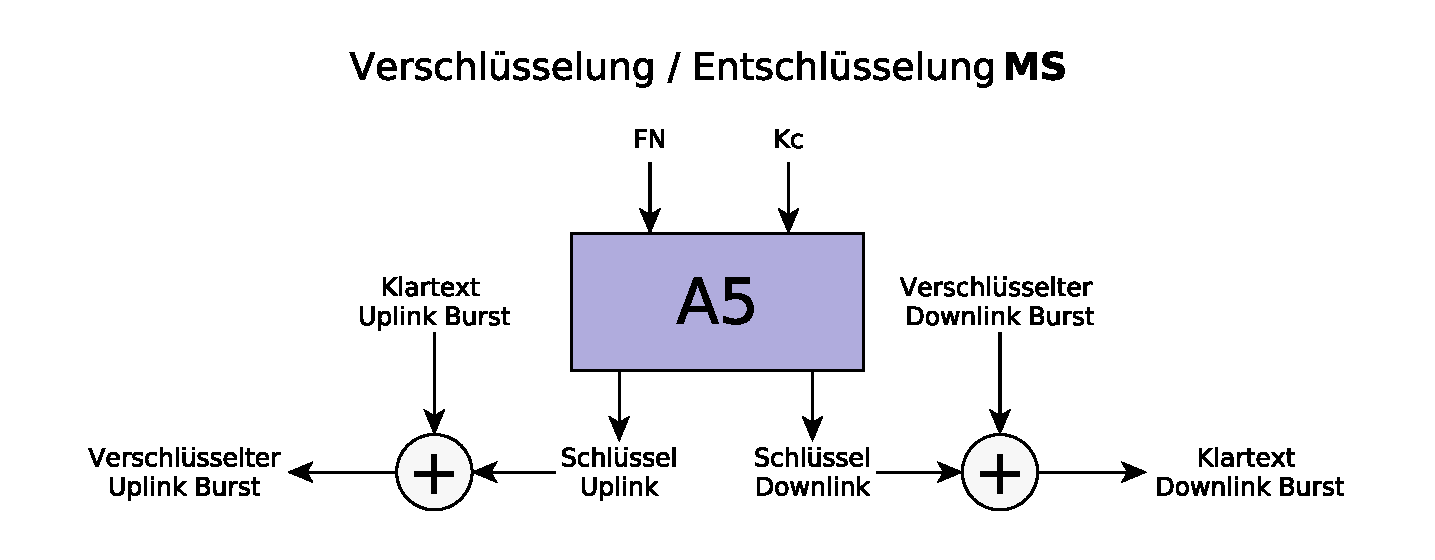
\includegraphics[width=1.0\textwidth]{figures/gsm_a5.pdf}
  \end{center}
  \caption[Der A5-Algorithmus]{Der \ac{A5}-Algorithmus, erstellt mit yEd nach \citepauthor[Abb. C.2]{3gpp:03.20}} \label{fig:a5-algorithm}
\end{figure}

Die \ac{MS} schickt der \ac{BTS} im \ac{CM} Service Request \citepauthor[Kap. 10.5.1.6]{3gpp:24.008} unter anderem das Mobile Station Classmark 2, welches ihre unterstützten Verschlüsselungsverfahren enthält. Die \ac{BTS} wählt daraus den größten gemeinsamen Nenner aus und informiert die \ac{MS} im \ac{CM} Service Accept \citepauthor[Kap. 9.2.5]{3gpp:24.008} über diesen. Durch die ebenfalls im Request übertragene \ac{CKSN} kann das Netzwerk überprüfen, ob schon ein übereinstimmender Security Context zwischen \ac{MS} und Netzwerk besteht, oder erst durch die Authentifizierung des Teilnehmers erstellt werden muss. Ist der beste gemeinsam verfügbare Algorithmus gefunden und \ac{Kc} bekannt, kann die Verbindung mit diesem geschützt werden. Die \ac{FN}, die mit in die Schlüsselstromgenerierung einfließt, verhindert Replay-Angriffe. Da diese nach einem Hyperframe allerdings wieder bei 0 beginnt und zumindest in einem laufenden Gespräch kein neuer Security Context zwischen \ac{MS} und \ac{BTS} ausgehandelt wird, wiederholt sich etwa alle drei Stunden und 26 Minuten der verwendete Schlüsselstrom. Für ein Gespräch, welches länger dauert entsteht dadurch ein Sicherheitsproblem, da der Schlüsselstrom wiederverwendet wird.
\begin{align}\label{eq:key-stream-reuse_1}
\begin{split}
&(A \oplus C) \oplus (B \oplus C) = (A \oplus B) \oplus (C \oplus C) = A \oplus B \\
\end{split}
\end{align}\noindent
\autoref{eq:key-stream-reuse_1} zeigt, dass bei Verwendung des gleichen Schlüsselstroms C für zwei verschiedene Klartextdatenströme A und B, deren \ac{XOR}-Kombination herausgefunden werden.
\begin{align}\label{eq:key-stream-reuse_2}
\begin{split}
&\text{A bekannt} \Rightarrow A \oplus A \oplus B  = B \\
&\text{B bekannt} \Rightarrow B \oplus B \oplus A = A 
\end{split}
\end{align}
Es gibt verschiedene Ansätze und Möglichkeiten, die Datenströme wieder voneinander zu trennen \citep[Kap. 3]{borisov2001intercepting}. \autoref{eq:key-stream-reuse_2} zeigt die Idee dahinter. Aus bekannten Teilen von A kann direkt der Inhalt dieses Teils von B hergeleitet werden und umgekehrt. 

Alle \ac{A5} Verschlüsselungsverfahren sind Stromchiffren und basieren auf der binären Addition des Datenstroms mit einem generierten Schlüsselstrom. In Anhang, in \autoref{hdl:a_a5} werden die von \ac{3GPP} für \ac{GSM} spezifizierten \ac{A5}-Verschlüsselungsverfahren kurz aufgeführt.

Laut Untersuchungen von \citet{gsmmap:secrep-ger} werden in deutschen 2G Netzen aktuell nur die Algorithmen A5/1 und A5/3 unterstützt. Dabei hat A5/1 bekannte Schwachstellen und A5/3 eine geringe Schlüssellänge die ihn verwundbar für Bruteforce Angriffe macht. Der aktuell (Stand 2017) als sicher geltende Algorithmus A5/4 \citep{3gpp:55.226} ist zwar seit einigen Jahren spezifiziert, wird aber nicht verwendet.

\begin{table}[H]
\centering
\begin{tabular}{|l|l|l|l|l|}
\rowcolor[HTML]{F7F7F7}
\hline
              & \textbf{O2} & \textbf{Eplus} & \textbf{Vodafone} & \textbf{Telekom} \\ \hline
\textbf{A5/1} & 73\%        & 56\%           & 41\%              & 26\%             \\ \hline
\textbf{A5/3} & 27\%        & 44\%           & 59\%              & 74\%             \\ \hline
\end{tabular}
\caption[Die prozentuale Verteilung der A5-Algorithmen in Deutschland]{Die prozentuale Verteilung der \ac{A5}-Algorithmen in Deutschland, aus \citep{gsmmap:secrep-ger}} \label{a5-usage-germany}
\end{table}

\subsection{Zusammenspiel der Sicherheitsalgorithmen in GSM}

\autoref{fig:encryption-overview} stellt das Zusammenspiel der Sicherheitsalgorithmen in \ac{GSM} dar. Aus \ac{Ki} und der im \ac{AKA} erhaltenen Challenge \ac{RAND}, berechnet das \ac{MS} mit \ac{A3} das Ergebnis \ac{RES} und schickt es an das Netzwerk zurück. Das Netzwerk vergleicht das Ergebnis des \ac{MS} mit dem eigenen als Authentizitätsprüfung. Aus den gleichen Eingangsparametern berechnet \ac{A8} auf beiden Seiten den Schlüssel \ac{Kc}. Nach erfolgreicher Authentifizierung und Aktivierung der Verschlüsselung wird aus \ac{Kc} und der aktuellen \ac{FN} der Schlüsselstrom für Uplink und Downlink generiert. Durch die \ac{XOR}-Verknüpfung mit den 114 verschlüsselten Nutzdatenbits eines dekodierten, eingehenden Burst kann dieser entschlüsselt werden. Durch die Verknüpfung mit dem unverschlüsselten Nutzdatenbits eines ausgehenden Bursts wird dieser verschlüsselt.

\begin{figure}[H]
  \begin{center}
    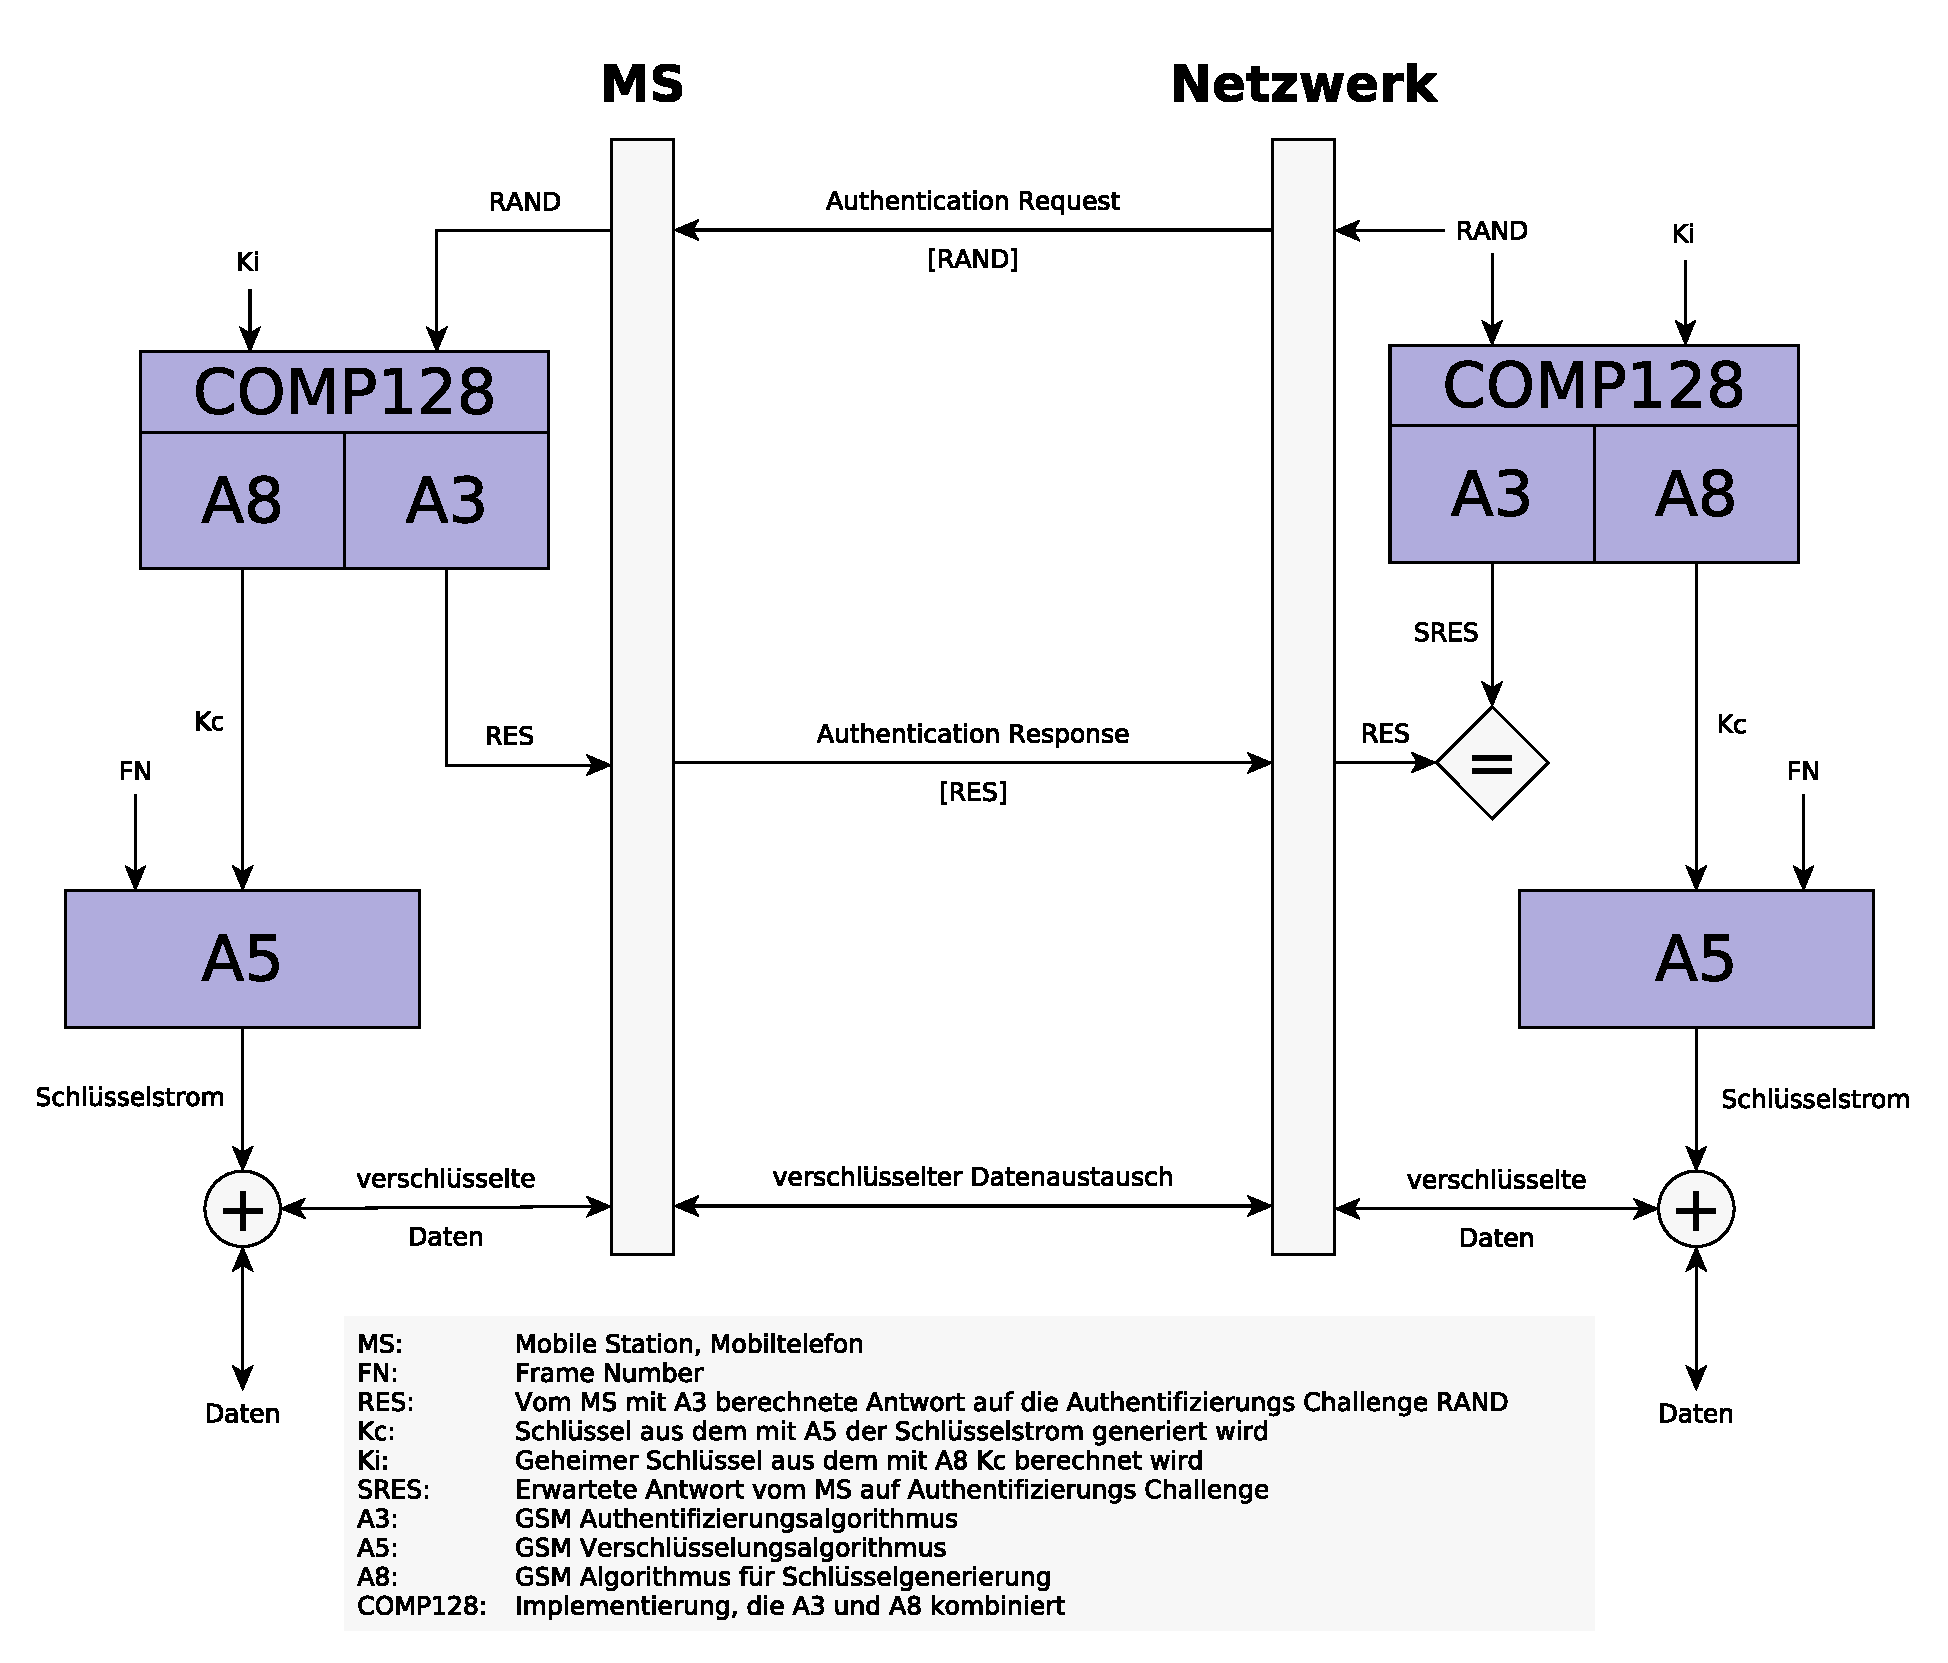
\includegraphics[width=1.0\textwidth]{figures/gsm_security_overview.pdf}
  \end{center}
  \caption[Das Zusammenspiel der GSM Sicherheitsalgorithmen]{Das Zusammenspiel der \ac{GSM} Sicherheitsalgorithmen, erstellt mit yEd} \label{fig:encryption-overview}
\end{figure}

\section{Timing Advance}\label{hdl:ta}

Da die Datenübertragung, abhängig von der Entfernung zwischen \ac{MS} und \ac{BTS}, unterschiedlich lange dauert, muss regelmäßig die Signallaufzeit gemessen und daraus der \ac{TA}-Wert \citepauthor[Kap. 6.1]{3gpp:04.04} berechnet werden. Dieser bestimmt, wie viel früher die \ac{MS} ihre Daten losschicken muss, damit sie zum richtigen Zeitpunkt bei der \ac{BTS} ankommen. Wird kein Timing-Advance verwendet, stimmt der Zeitpunkt der Ankunft des Signals unter Umständen nicht mit dem Anfang eines \ac{TDMA}-Zeitschlitzes überein. Damit liegt die Nachricht außerhalb eines gültigen physikalischen und logischen Kanals und kann von der \ac{BTS} nicht richtig dekodiert werden. Auf der Seite des \ac{MS} wird die zeitliche Verzögerung bei der Synchronisation mit der \ac{BTS} berücksichtigt, weshalb dort die Nachrichten in den korrekten Zeitschlitzen ankommen.

Der erste \ac{TA}-Wert wird dem \ac{MS} in der "`Immediate Assignment"' Nachricht auf dem \ac{AGCH} mitgeteilt und während einer Verbindung auf dem \ac{SACCH} aktualisiert. Der \ac{TA}-Wert ist quantisiert durch Vielfache der Bitübertragungsdauer von $3,7\mu s$. Er kann Werte zwischen 0 und 63 annehmen, wodurch sich der Sendezeitpunkt maximal um $63 \cdot 3.7\mu = 233\mu s$ verschieben lässt. Das entspricht etwas weniger als einem halben Burst. Das elektromagnetische Funksignal breitet sich mit Lichtgeschwindigkeit aus. In der Zeit von $233\mu s$ wird also ein Weg von ca. $300.000 \nicefrac{km}{s} \cdot 233 \cdot 10^{-6} s = 69.9 km$ zurückgelegt, womit sich ein maximaler Abstand vom \ac{MS} zur \ac{BTS} von etwa $35km$ realisieren lässt.
	\chapter{Osmocom} \label{hdl:grundlagen_osmocom}
Das \textbf{O}pen \textbf{S}ource \textbf{MO}bile \textbf{COM}munications Projekt ist ein Umbrella-Projekt für freie und quelloffene Software im Bereich der mobilen Telekommunikation. Es umfasst Software und Werkzeuge, die eine Vielzahl von mobilen Kommunikationsstandards wie \ac{GSM}, \ac{UMTS}, \ac{DECT} und \ac{TETRA} implementieren \citep{osmocom}.

Die unter Osmocom vereinigten Projekte werden vom Unternehmen sysmocom\footnote{\url{https://www.sysmocom.de/}} und freien Entwicklern aktiv gepflegt. Der Gründer von Osmocom, wie auch sysmocom ist Harald Welte. Es gibt eine aktive Community, Mailinglisten und in Redmine gepflegte Repositories der verschiedenen Projekte.

Die Software findet im akademischen Bereich Verwendung. Aufgrund des quelloffenen Codes und der vielen Anwendungsmöglichkeiten eignet sie sich, um einen Einblick in die Welt der mobilen Kommunikation zu bekommen \citep{osmocom:bb-project-rationale}.

Kommerziell genutzt werden die Projekte osmoBSC und osmoBTS zum Beispiel von Rhizomatica\footnote{\url{https://www.rhizomatica.org}}, um in Mexiko Bergregionen an ein \ac{GSM}-Netz anzubinden \citep{osmocom:news-rhizomatica}. In der maritimen Telekommunikation bietet On-Waves\footnote{\url{https://www.on-waves.com}} auf OsmoBTS, OsmoPCU und OsmoBSC basierende Lösungen an, um Schiffe mit einem \ac{GSM}-Netz abzudecken \citep{osmocon:onwaves}. Für zwei aktuelle Projekte von Facebook wird ebenfalls Osmocom Technologie verwendet. OpenCellular nutzt osmoBTS und hat die Entwicklung einer robusten Basisstation für den Einsatz in klimatisch anspruchsvollen Regionen zum Ziel \citep{osmocon:opencellular}. Der "`Community Cellular Manager"' soll ein Verwaltungssystem und Abrechnungsmöglichkeiten für mehrere privat verwaltete Netzwerkzellen liefern und implementiert eine Schnittstelle zu osmoBSC \citep{osmocon:communityCellularManager}.

Es gibt mehrere Osmocom Bibliotheken, die in Projekten gemeinsam genutzte Funktionen beinhalten \citep{osmocom:libraries}. Für Debian sind aktuelle Nightly Builds der am häufigsten benutzten Bibliotheken verfügbar \citep{osmocom:nightly-builds}.

Die Projekte, die für den Aufbau eines funktionierenden \ac{GSM}-Netzwerks benötigt werden, werden in den folgenden Kapiteln erklärt. 

\section{OsmocomBB} \label{hdl:grundlagen_osmocom_OsmocomBB}
OsmocomBB ist eine Open-Source \ac{GSM}-Baseband Implementierung. Das Projekt wurde mit dem Ziel gestartet, proprietäre \ac{GSM}-Baseband Software vollständig zu ersetzen. Es implementiert Treiber für interne und externe, analoge und digitale \ac{GSM} Baseband Peripheriegeräte und den \ac{MS} seitigen \ac{GSM}-Protokollstapel von Schicht 1 bis 3. \citep{osmocom:bb}

Mit OsmocomBB ist es also möglich, auf der Basis von freier Software Mobilfunkdienste (Anrufe, \ac{SMS}) auf einem kompatiblem Handy zu nutzen.

Alle Informationen zum Projekt findet man im Osmocom Wiki\footnote{\url{https://osmocom.org/projects/baseband/wiki}}.

\section{OsmoBTS} \label{hdl:grundlagen_osmocom_OsmoBTS}

OsmoBTS realisiert eine \ac{GSM}-\ac{BTS} in Open-Source. Damit implementiert das Projekt den Protokollstapel der Abis-Schnittstelle zum \ac{BSC} und den netzwerkseitigen Protokollstapel der \ac{Um}-Schnittstelle. Was das Projekt besonders macht ist die Unterstützung einer Vielzahl verschiedener Transceiverhardware und Implementierungen der physikalischen Schicht. OsmoBTS kann zum Beispiel zusammen mit OsmoTRX verwendet werden, um \ac{SDR}-Geräte, wie die \acp{USRP} aus dem Angebot von Ettus Research\footnote{\url{https://www.ettus.com/}}, als Transceiver zu verwenden. \citep[OsmoBTS Benutzerhandbuch]{osmocom:docs-latest}

Die Konfiguration des \ac{BTS} ist zur Laufzeit über ein \ac{VTY} \ac{CLI} möglich.

Alle Informationen zum Projekt findet man im Wiki\footnote{\url{https://osmocom.org/projects/osmobts/wiki/Wiki}} und im Benutzerhandbuch.

\section{OsmoBSC und OsmoNITB} \label{hdl:grundlagen_osmocom_OpenBSC}

OsmoBSC implementiert einen \ac{GSM}-\ac{BSC} und somit den Protokollstapel der Abis-Schnittstelle zur \ac{BTS} und der A-Schnittstelle zum \ac{MSC}. \citep[OsmoBSC Benutzerhandbuch]{osmocom:docs-latest}

Alle Informationen zu OsmoBSC findet man im Wiki\footnote{\url{https://osmocom.org/projects/openbsc/wiki/Osmo-bsc}} und im Benutzerhandbuch.

\acused{NITB}
OsmoNITB implementiert einen \ac{GSM}-\ac{BSC} als "`Network in the Box"'. Das Projekt realisiert die vollständige Abis-Schnittstelle zur \ac{BTS}, enthält jedoch intern alle nötigen Netzkomponenten und implementiert daher keine A-Schnittstelle. Mit dem \ac{NITB} ist es möglich ein in sich funktionales Netzwerk, bestehend aus dem \ac{NITB} selbst und einer Reihe von angebundenen \ac{BTS}, aufzubauen. \citep[OsmoNITB Benutzerhandbuch]{osmocom:docs-latest}

Alle Informationen zu OsmoNITB findet man im Wiki\footnote{\url{https://osmocom.org/projects/osmonitb/wiki/OsmoNITB}} und im Benutzerhandbuch.

Die Konfiguration von \ac{BSC} und \ac{NITB} ist zur Laufzeit über ein \ac{VTY} \ac{CLI} möglich.

	\input{misc/emptypage}
	%%%%%%%%%%%%%%%%%%%%%%%%%%%%%%%%%%%%%%%%%%%%%%%%%%%%%%%%%%%
%%% Umsetzung
%%%%%%%%%%%%%%%%%%%%%%%%%%%%%%%%%%%%%%%%%%%%%%%%%%%%%%%%%%%
\chapter{Die theoretische Ausarbeitung des Angriffs} \label{hdl:theroetical-attack}

In diesem Kapitel wird der \ac{MitM} Angriff theoretisch ausgearbeitet und gezeigt, unter welchen Voraussetzungen er in \ac{GSM} umgesetzt werden kann. Die Schwachstellen im \ac{GSM}-Standard, die den Angriff möglich machen werden dargestellt und die Schritte herausgearbeitet, die notwendig sind um ein ausgehendes Telefonat erfolgreich umzuleiten.

\section{Das Problem von Stromverschlüsselung ohne Integrität} \label{hdl:einleitung_verschlue_ohne_int}

\ac{GSM} verwendet Stromverschlüsselung zum Schutz der vertraulichen Kommunikation und ist damit anfällig für "`Known Plaintext"' Angriffe ohne Kenntnis des kryptografischen Schlüssels. Da die Integrität der übertragenen Nachrichten nicht geschützt, ist kann ein \ac{MitM}-Angreifer bekannte Daten beliebig verändern.

\begin{figure}[H]
	\centering 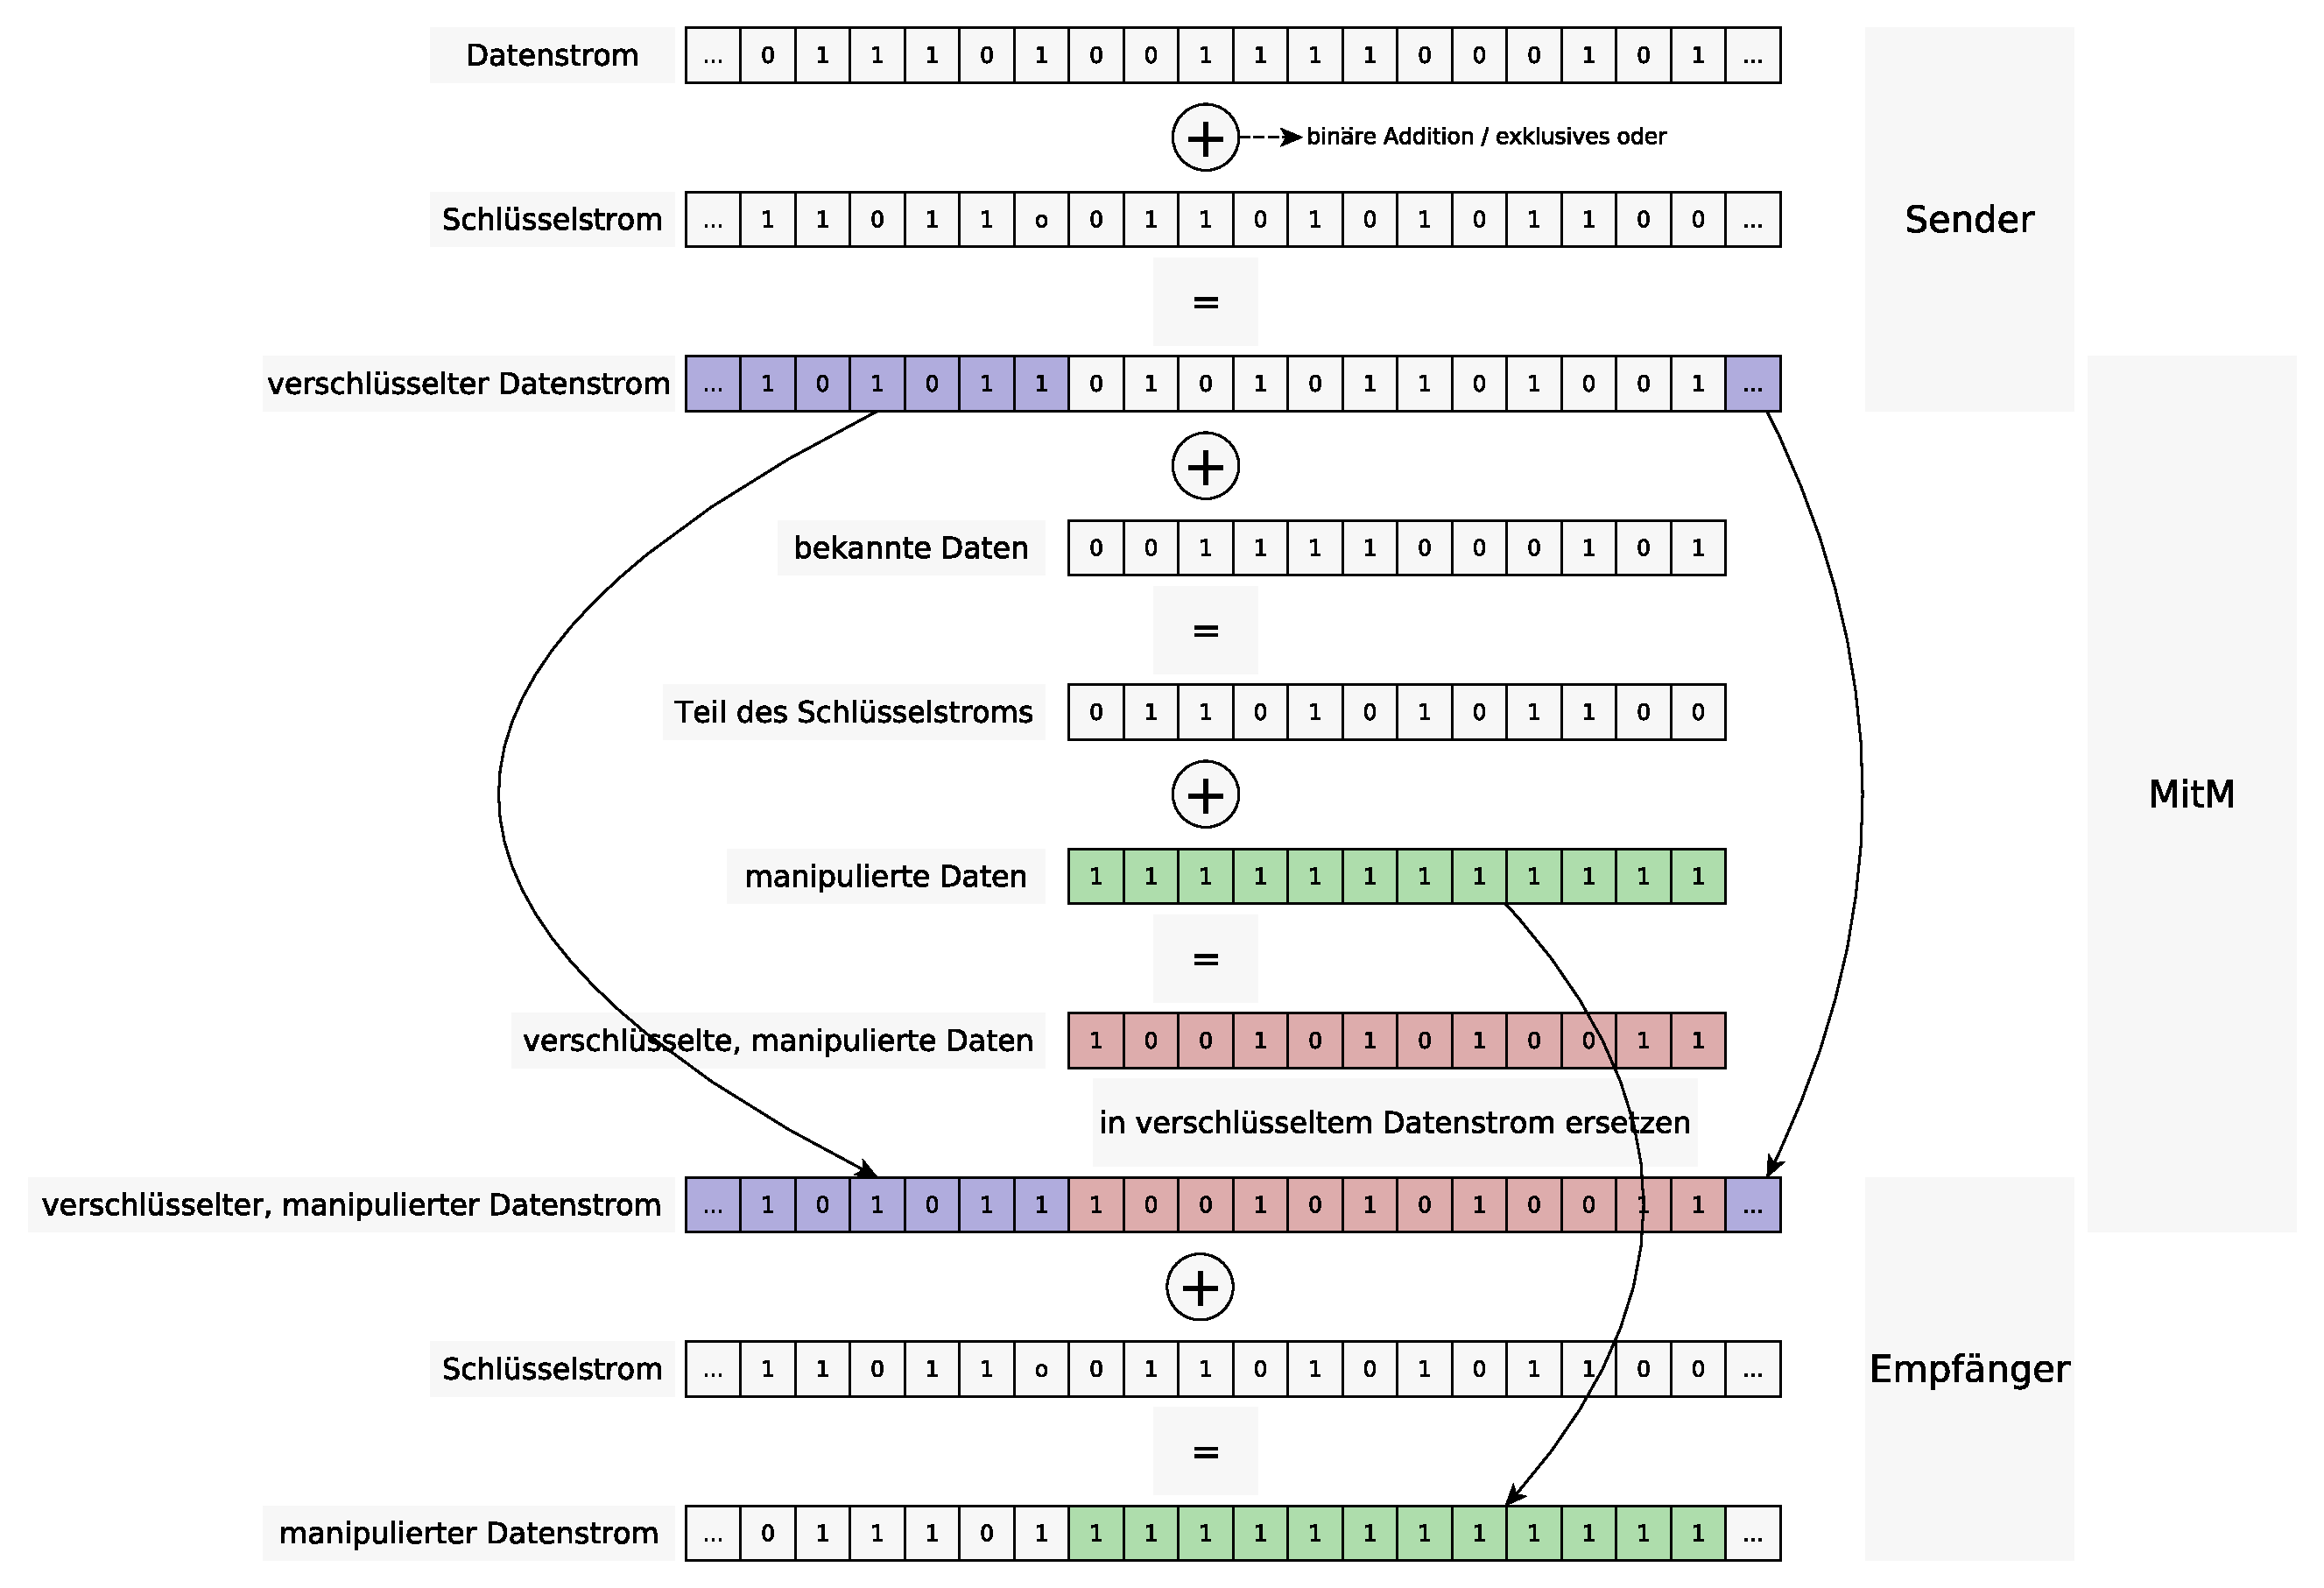
\includegraphics[width=1.0\linewidth]{figures/partially_known_plaintext_manipulation.pdf}
	\caption[Datenmanipulation ohne Kenntnis des kryptografischen Schlüssels]{Datenmanipulation ohne Kenntnis des kryptografischen Schlüssels, erstellt mit yEd} \label{fig:partially-known-plaintext-manipulation}
\end{figure}

\autoref{fig:partially-known-plaintext-manipulation} zeigt an einem Ausschnitt des Datenstroms, wie bekannte Daten trotz Verschlüsselung von einem \ac{MitM} geändert werden können. Da der Chiffrestrom das Ergebnis der \ac{XOR}-Kombination von Datenstrom und Schlüsselstrom ist, kann der Angreifer für bekannte Daten, den verwendeten Schlüsselstrom berechnen. Die Kenntnis des Schlüsselstroms für einen Teil des Datenstroms erlaubt dem Angreifer, diesen Teil beliebig zu manipulieren. Beim Empfänger kommt nach der Entschlüsselung der geänderte Datenstrom heraus. Methoden zum Schutz der Integrität übertragen zusätzlich zu den Nutzdaten in der Regel einen Hashwert, der nur korrekt berechnet werden kann, wenn der vollständige Klartext bekannt ist. Änderungen eines Angreifers, der nur einen Teil der Daten kennt, können also vom Empfänger bemerkt werden. Ohne Methoden zum Schutz der Integrität kann der Empfänger die Manipulation hingegen nicht bemerken.

Die Kenntnis über den mangelnden Schutz von Verschlüsselung ohne Integrität ist weit verbreitet. Dennoch werden darauf basierende Angriffe von verschiedenen Übertragungsprotokollen und deren Spezifikationen ermöglicht. So zeigen \citet{paterson2006cryptography} die Schwachstelle in der \ac{IPSec} Implementierung im Linux Kernel auf. Sie können, wenn \ac{IPSec} ohne Authentifizierung und Integrität konfiguriert ist, die Verschlüsselung von \ac{ESP} Paketen erfolgreich brechen. \citet{degabriele2007attacking} stellen mehrere implementierungsunabhängige Angriffe auf \ac{IPSec} vor und zeigen damit, dass die Schwachstelle in \ac{IPSec} nicht nur im Linux Kernel existiert, sondern in der \ac{IPSec}-Standardisierung. Der für den Standard IEEE 802.11 für Drahtlosnetzwerke spezifizierte Verschlüsselungsalgorithmus \ac{WEP}, leidet an der gleichen Schwachstelle. Er gilt heute offiziell als unsicher, von Herstellern wird generell empfohlen, \ac{WEP} nicht mehr für ihre Geräte zu verwenden. Dennoch besteht nach wie vor die Möglichkeit, die meisten Wlan-Router und andere IEEE 802.11 kompatible Geräte für \ac{WEP} zu konfigurieren. \citet{bittau2006final} stellen einen Fragmentierungsangriff auf \ac{WEP} vor, der wegen seiner kurzen Ausführungszeit, trotz regelmäßiger Erneuerung des Schlüssels funktioniert. Wiederum basiert er auf fehlender Integrität von durch Stromverschlüsselung geschützten Daten. Die Arbeiten weisen alle auf die Gefahren der Nutzung von Verschlüsselung ohne Integrität hin und empfehlen, solche Konfigurationen generell nicht zu unterstützen und zu verwenden.

\section{Die Idee des \acl{MitM} Angriffs auf GSM} \label{hdl:einleitung_mitm-gsm}

\begin{figure}[H]
	\centering 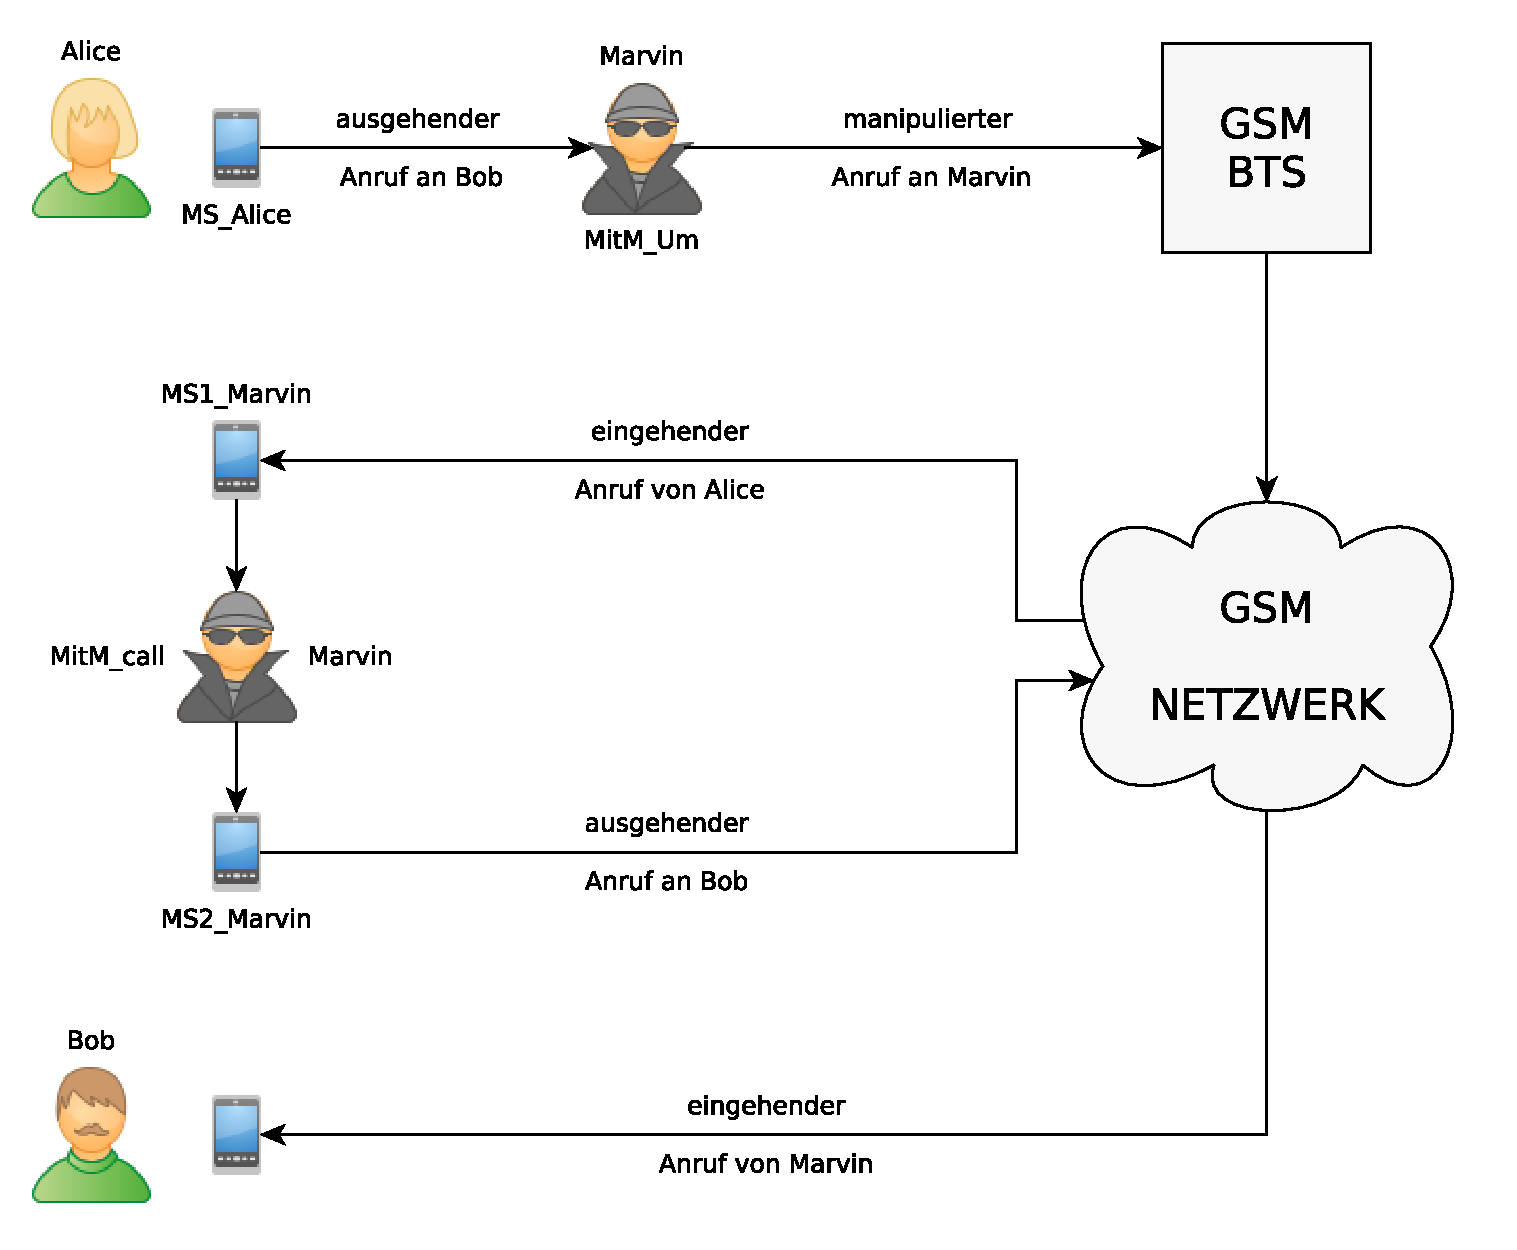
\includegraphics[width=0.9\linewidth]{figures/mitm_attack_overview.pdf}
	\caption[Die Idee des MitM-Angriffs]{Die Idee des \ac{MitM}-Angriffs, erstellt mit yEd} \label{fig:mitm-attack-overview}
\end{figure}

Das Szenario (siehe \autoref{fig:mitm-attack-overview}):

Alice ist mit dem \ac{GSM}-Netz verbunden und möchte Bob anrufen. Der Angreifer Marvin hat ein \ac{MitM}-Gerät ($\ac{MitM}_{Um}$) auf der \ac{Um} Schnittstelle installiert, mit dem er auf physikalischer Ebene Zugriff auf alle ausgetauschten Nachrichten zwischen Alice's Telefon und der \ac{GSM}-\ac{BTS} hat. Die Nachrichten sind kodiert und stromverschlüsselt. Stromverschlüsselung schützt nicht vor Datenmanipulation bei bekanntem Klartext und Bob's Telefonnummer ist Marvin bekannt. Er kann deshalb den Anrufaufbau im $\ac{MitM}_{Um}$ manipulieren und Bob's Telefonnummer austauschen. Da die Integrität der ausgetauschten Nachrichten in \ac{GSM} nicht geschützt ist, können weder Alice noch die \ac{BTS} die Manipulation bemerken. Der manipulierte Anruf wird deshalb vom Netzwerk als gültig erkannt und an Marvin's Mobiltelefon weitergeleitet. Das Netzwerk übernimmt Kodierung und Verschlüsselung des übertragenen Datenstroms, Marvin erhält das Gespräch von Alice im Klartext. Marvin ruft nun Bob an und verknüpft die beiden Anrufe so, dass Bob die Gesprächsdaten von Alice erhält und umgekehrt. Da Marvin Zugriff auf den Klartext beider Datenströme hat, kann er diese aufnehmen und manipulieren. Der dadurch entstandene \ac{MitM}-Angriff ($\ac{MitM}_{call}$) funktioniert unabhängig vom verwendeten Verschlüsselungsverfahren und ist in \autoref{fig:mitm-in-voice-con} dargestellt.

\begin{figure}[H]
	\centering 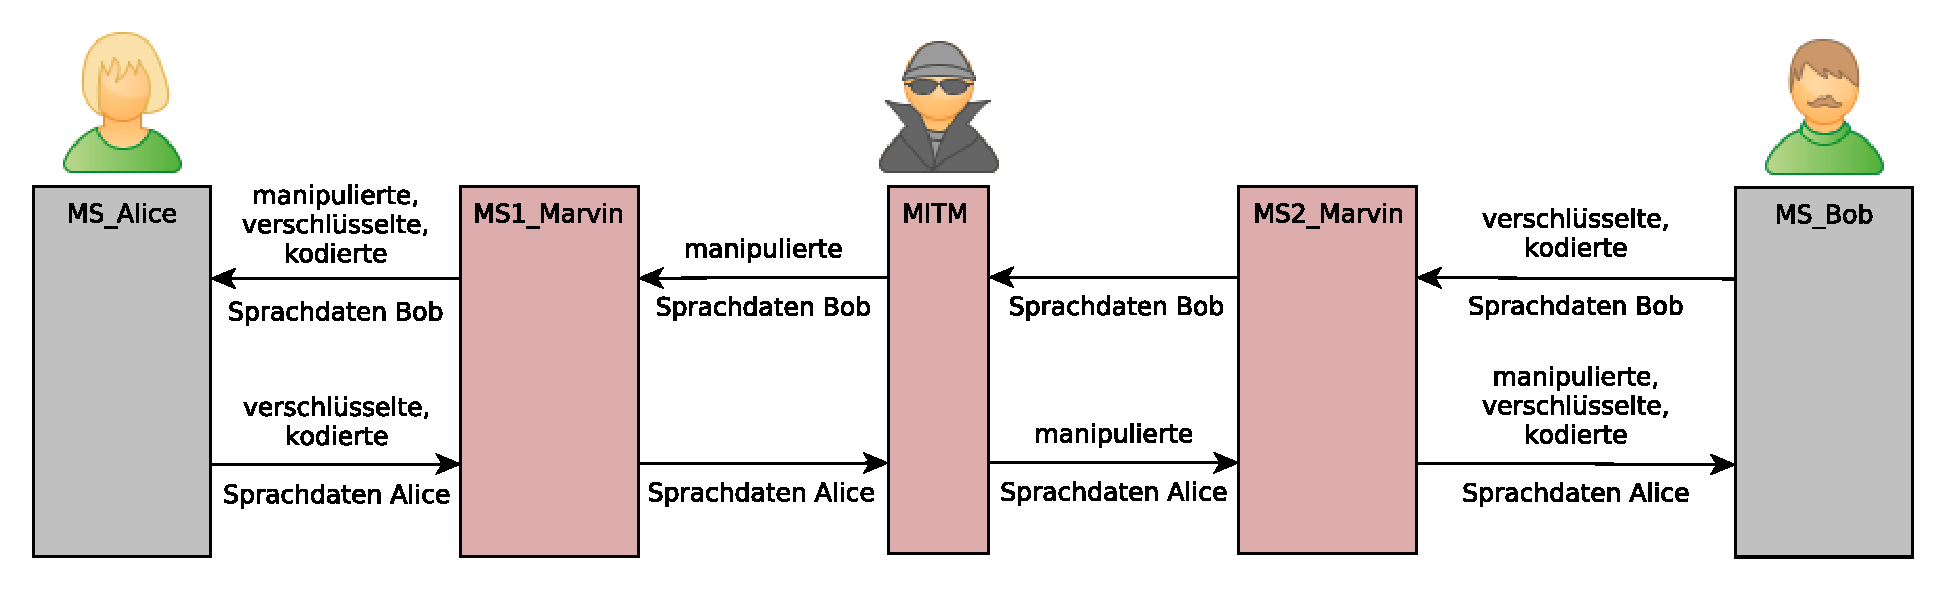
\includegraphics[width=1.0\linewidth]{figures/mitm_in_voice_connection.pdf}
	\caption[Der entwickelte MitM-Angriff auf eine Sprachverbindung]{Der entwickelte \ac{MitM}-Angriff auf eine Sprachverbindung, erstellt mit yEd} \label{fig:mitm-in-voice-con}
\end{figure}

Dass ein \ac{MitM}-Angriff auf dem \ac{Um} möglich ist, haben bereits \citet{barkan2003instant}, \citet{meyer2004man} und \citet{paget2010practical} gezeigt. Für ihre \ac{MitM}-Angriffe verwenden sie eine falsche Basisstation (siehe \autoref{hdl:einleitung_stand-der-technik}). Das \ac{MitM}-Gerät für den vorgestellten Angriff benötigt nur Zugriff auf den verschlüsselten, kodierten Datenverkehr und muss den kryptografischen Schlüssels nicht berechnen. Statt einer falschen Basisstation reicht also ein \ac{MitM}-Gerät auf physikalischer Ebene, mit geringer Rechenleistung aus. Das würde in etwa der Funktionalität eines \ac{GSM}-Repeaters mit zusätzlichen Verarbeitungsroutinen für den Datenstrom entsprechen. Statt Daten nur zu verstärken und weiterzuleiten kann er diese auch analysieren und manipulieren. Die Zeit dafür kann durch die Verzögerung des Datenverkehrs von bis zu $233 \mu s$ gewonnen werden, die die Timing Advance Funktion des \ac{GSM}-Standards erlaubt (siehe \autoref{hdl:ta}). Das \ac{MitM}-Gerät in der Funkschnittstelle, mit Zugriff auf den verschlüsselten und kodierten Datenverkehr, wird in dieser Arbeit vorausgesetzt. Die Möglichkeiten der Nutzung eines modifizierten \ac{GSM}-Repeaters für den \ac{MitM}-Angriff werden nicht untersucht.

\section{Analyse des Nachrichtenflusses auf der Um Schnittstelle beim Anrufaufbau}\label{hdl:call-setup-message-flow-analysis}

Um herauszufinden, welche Nachrichten für den Aufbau einer Telefonverbindung zuständig sind, wird der Nachrichtenfluss auf der Um Schnittstelle analysiert. Folgende Fragen müssen beantwortet werden:
\begin{itemize}
\item Wie wird das Opfer identifiziert?
\item Wie wird die für den Anrufaufbau zuständige "`Setup"' Nachricht im Nachrichtenfluss identifiziert?
\end{itemize}

\autoref{fig:moc-um-1} und Folgende enthalten die zwischen \ac{MS} und \ac{BTS} ausgetauschten Signalisierungsnachrichten. Aktuelle (Stand 2015) Informationen zum untersuchten Nachrichtenfluss finden sich in \citetauthor[Kap. 7.3.2]{3gpp:23.108} und \citetauthor[Abb. A.1]{3gpp:24.007}. Übertragene \ac{RR}-Signalisierungsnachrichten sind in \citetauthor{3gpp:04.18}, \ac{MM} und \ac{CM}-Nachrichten, sowie Service-Requests in \citetauthor{3gpp:24.008} spezifiziert.

\begin{figure}[H]
	\centering \includegraphics[width=1.0\textwidth]{figures/mscgen/gsm_MOC_on_UM01.pdf}
	\caption[Nachrichtenfluss auf der Um-Schnittstelle beim Anrufaufbau, Teil 1]{Nachrichtenfluss auf der \ac{Um}-Schnittstelle beim Anrufaufbau, Teil 1, nach \citepauthor[Kap. 7.3.2]{3gpp:23.108} und \citepauthor[Abb. A.1]{3gpp:24.007}} \label{fig:moc-um-1}
\end{figure}

\begin{description}
\item[1:] Das \ac{MS} beantragt mit dem \texttt{CHANNEL-REQUEST} \citepauthor[Kap. 9.1.8]{3gpp:04.18} einen dedizierten Kanal. Der Request enthält ein Flag, das dem Netzwerk signalisiert, für was der Kanal verwendet werden soll. Bei "`Very Early Assignment"' reserviert das Netzwerk an dieser Stelle einen \ac{TCH}. Das bedeutet, die folgende Signalisierung würde auf dem \ac{FACCH} und nicht wie in der Abbildung auf dem \ac{SDCCH} erfolgen \citepauthor[Kap. 7.3.2]{3gpp:23.108}. Mit dem \texttt{IMMEDIATE-ASSIGNMENT} \citepauthor[Kap. 9.1.18]{3gpp:04.18} erhält das \ac{MS} vom Netzwerk die benötigten Informationen zum reservierten Kanal, was es ihm ermöglicht, auf diesen zu wechseln. Nach dem Wechsel in den "`Dedicated Mode"' beantragt das \ac{MS} auf dem \ac{SDCCH} mit einem \ac{SABM}-Frame den Wechsel vom unacknowledged in den asynchronous balanced \ac{LAPDm}-Modus. Damit initiiert es den Aufbau einer von der Datensicherungsschicht geschützten Verbindung (siehe \autoref{hdl:einfuehrung-gsm_schnittstellen_protokolle-um_interface-layer2}). Das \ac{SABM}-Frame trägt den \texttt{CM-SERVICE-REQUEST} \citepauthor[Kap. 9.2.9]{3gpp:24.008} mit der \ac{IMSI} oder \ac{TMSI} des Netzteilnehmers, dem Typ des angeforderten \ac{CM}-Dienstes und Informationen zu \ac{MS}-seitig unterstützten Verschlüsselungsverfahren mit sich. Der Empfang der \ac{SABM}-Nachricht und der netzwerkseitige Wechsel in den asynchronous balanced Mode, wird durch ein \ac{UA}-Frame mit einer Kopie des erhaltenen Service-Requests bestätigt. Alle weiteren Signalisierungsnachrichten auf dem dedizierten Kanal sind in \ac{I}-Frames verpackt und werden bei erfolgreichem Empfang mit einem \ac{RRm}-Frame bestätigt. Das \ac{RRm}-Frame hat in dem Fall nichts mit \acl{RR} zu tun, sondern ist eine Kontrollnachricht des \ac{LAPDm}-Protokolls. Die Werte der Zähler \ac{N(R)} und \ac{N(S)} für empfangene und gesendetet Nachrichten sind im Flussdiagramm für \ac{I} und \ac{RRm}-Frames dargestellt.
\item[2:] Die Identitätsabfrage des Netzteilnehmers \citep[Kap. 4.3.3]{3gpp:24.008} erfolgt, wenn das Netzwerk die \ac{TMSI} aus dem \texttt{CM-SERVICE-REQUEST} keiner \ac{IMSI} zuweisen kann. Sie sollte nur wenn nötig ausgeführt werden, um die Anonymität der Netzteilnehmer zu schützen, also in der Regel nicht bei jeder Anfrage eines Teilnehmers. Der \texttt{IDENTITY-REQUEST} \citep[Kap. 9.2.10]{3gpp:24.008} enthält den Identitätstyp, der abgefragt wird (\ac{IMSI}, \ac{TMSI}, \ac{IMEI}). Das Netzwerk kann mehr als einen Identity Request schicken um weitere Identitäten anzufordern. Nachdem die \ac{MS} den Request mit einer \texttt{IDENTITY-RESPONSE} \citep[Kap. 9.2.11]{3gpp:24.008} beantwortet und die gewünschte Identität geliefert hat, ist die Routine abgeschlossen.
\item[3:] Wie die Identitätsabfrage erfolgt auch die Authentifizierung nur bei Bedarf. Aus dem \texttt{CM"=SERVICE"=REQUEST} kennt das Netzwerk die aktuellen Sicherheitsparameter des \ac{MS} und kann mit diesen überprüfen, ob ein gültiger Security-Context besteht (siehe \autoref{hdl:keygen}). Existiert kein gültiger Security-Context muss das \ac{AKA} erneut durchgeführt werden, ansonsten kann die Authentifizierung übersprungen werden. Wenn \ac{MS} und \ac{AuC} \ac{UMTS}-fähig sind, wird das \ac{UMTS}-\ac{AKA} ausgeführt (siehe \autoref{hdl:umts-aka}), andernfalls das \ac{GSM}-\ac{AKA} (siehe \autoref{hdl:authentication}). Die ausgetauschten Nachrichten unterscheiden sich dabei nur in der Interpretation des Inhalts von \ac{RES} und \ac{RAND}. Das Netzwerk schickt dem \ac{MS} im \texttt{AUTHENTICATION-REQUEST} \citep[Kap. 9.2.2]{3gpp:24.008}, je nach verwendetem \ac{AKA}, die \ac{GSM} oder \ac{UMTS} Challenge \ac{RAND}. Das \ac{MS} berechnet die Antwort auf die Challenge und schickt sie dem Netzwerk in der \texttt{AUTHENTICATION-RESPONSE} \citep[Kap. 9.2.2]{3gpp:24.008} zurück. Ist die Authentifizierung erfolgreich, kennen beide Seiten auch den synchronen, kryptografischen Schlüssel für das A5 Verschlüsselungsverfahren.
\end{description}

\begin{figure}[H]
	\centering \includegraphics[width=1.0\linewidth]{figures/mscgen/gsm_MOC_on_UM02.pdf}
	\caption[Nachrichtenfluss auf der Um-Schnittstelle beim Anrufaufbau, Teil 2]{Nachrichtenfluss auf der \ac{Um}-Schnittstelle beim Anrufaufbau, Teil 2, nach \citepauthor[Kap. 7.3.2]{3gpp:23.108} und \citepauthor[Abb. A.1]{3gpp:24.007}} \label{fig:moc-um-2}
\end{figure}

\begin{description}
\item[4:] Mit dem \texttt{CIPHERING-MODE-COMMAND} \citep[Kap. 9.1.9]{3gpp:04.18} befiehlt das Netzwerk dem \ac{MS}, von jetzt an die Verschlüsselung des Uplinks zu starten. Sobald die korrekt verschlüsselte \texttt{CIPHERING-MODE-COMPLETE} \citep[Kap. 9.1.10]{3gpp:04.18} Bestätigung des \ac{MS} empfangen wird, beginnt das Netzwerk den Downlink zu verschlüsseln. Der darauf folgende Nachrichtenverkehr auf dem dedizierten Kanal ist bidirektional durch das ausgehandelte, synchrone Verschlüsselungsverfahren (zum Beispiel A5/3) geschützt.
\item[5:] Mit dem Call \texttt{SETUP} \citep[Kap. 9.3.23.2]{3gpp:24.008} wird der Anruf vom \ac{MS} initiiert. Die angerufene Nummer und weitere Informationen zum Anruf werden dem Netzwerk erst in dieser Nachricht mitgeteilt. Um den Anruf umzuleiten, muss also die \texttt{SETUP}-Nachricht manipuliert werden. Mit \texttt{CALL-PROCEEDING} \citep[Kap. 9.3.3]{3gpp:04.18} wird dem \ac{MS} signalisiert, dass das Netzwerk das \texttt{SETUP} erhalten hat und den Anruf bearbeitet.
\item[6:] Bei "`Early Assignment"' erfolgt, direkt nach dem \texttt{CALL-PROCEEDING}, der Wechsel vom \ac{SDCCH} auf den \ac{TCH}. Er wird durch einen \texttt{ASSIGNMENT-COMMAND} \citep[Kap. 9.1.2]{3gpp:04.18} initiiert. Auf dem \ac{TCH} wird für die weitere Signalisierung eine zuverlässige Verbindung benötigt, die mit den \ac{LAPDm}-Frames \ac{SABM} und \ac{UA} aufgebaut wird. Die Frames tragen diesmal keine Informationen höherer Schichten mit sich, der \texttt{CM-SERVICE-REQUEST} wurde ja bereits übertragen. Mit dem \texttt{ASSIGNMENT-COMPLETE} teilt das \ac{MS} dem Netzwerk mit, dass es erfolgreich den Kanal gewechselt hat.
\end{description}

\begin{figure}[H]
	\centering \includegraphics[width=1.0\linewidth]{figures/mscgen/gsm_MOC_on_UM03.pdf}
	\caption[Nachrichtenfluss auf der Um-Schnittstelle beim Anrufaufbau, Teil 3]{Nachrichtenfluss auf der \ac{Um}-Schnittstelle beim Anrufaufbau, Teil 3, nach \citepauthor[Kap. 7.3.2]{3gpp:23.108} und \citepauthor[Abb. A.1]{3gpp:24.007}} \label{fig:moc-um-3}
\end{figure}

\begin{description}
\item[7:] Mit \texttt{PROGRESS}-Nachrichten \citep[Kap. 9.3.17]{3gpp:24.008} wird das \ac{MS} mit Informationen zum aktuellen Stand der Bearbeitung des Anrufs versorgt. \texttt{PROGRESS} kann während des Anrufaufbaus mehrfach verschickt werden \citep[Kap. 5.5.6]{3gpp:24.008}.
\item[8:] Erhält das \ac{MS} ein \texttt{ALERTING} \citep[Kap. 5.2.1.5]{3gpp:24.008} vom Netzwerk, wurde der Anruf durchgestellt und es klingelt beim angerufenen Netzteilnehmer. Dem Anrufer wird das durch Abspielen des Freizeichens signalisiert.
\item[9:] Wenn der angerufene Netzteilnehmer abgehoben hat, wird dem \ac{MS} das mit einer \texttt{CONNECT}-Nachricht mitgeteilt. Das \ac{MS} bestätigt diese mit einer \texttt{CONNECT"=ACKNOWLEDGE}-Nachricht und wechselt in den "`call-active"' State. Die beiden Gesprächspartner sind jetzt erfolgreich miteinander verbunden und auf dem \ac{TCH} werden ihre Sprachdaten übertragen.
\end{description}
Obiger Ablauf wurde mit der Aufzeichnung eines ausgehenden Anrufs mit Wireshark verifiziert. Der Anruf erfolgte von einem mit OsmocomBB gesteuerten Motorola C123 über eine reguläre E-Plus \ac{BTS}. Der analysierte Mitschnitt wurde von OsmocomBB erstellt und kann im Anhang in \autoref{lst:real_bts_traffic_det_wireshark} eingesehen werden. 

\textbf{Ergebnis}:

Das Opfer kann im \texttt{CM-SERVICE-REQUEST} identifiziert werden, da in diesem seine Identität in Form der \ac{TMSI} oder \ac{IMSI} enthalten ist. Der \texttt{CM-SERVICE-REQUEST} ist Teil des \ac{MM} und wird vom \ac{SABM} huckepack getragen (piggybacking). Der \ac{SABM} ist unverschlüsselt, die Nachrichten können somit vom $\ac{MitM}_{Um}$ nach der Identität des Opfers gefiltert werden. Da die \ac{TMSI} nur die temporäre Identität eines Netzteilnehmers ist, muss sie seiner eindeutigen Identität (\ac{IMSI} oder \ac{MSISDN}), zugeordnet werden. Dazu gibt es zwei Möglichkeiten:
\begin{itemize}
\item \textbf{Silent \ac{SMS}}: Eine "`lautlose"' \ac{SMS} wird an die Telefonnummer des Opfers geschickt und der \ac{PCH} des \ac{BTS}, in dessen Zuständigkeitsbereich es sich befindet, auf Paging Nachrichten abgehört. Die \ac{TMSI}, die über die eingehende \ac{SMS} benachrichtigt wird, gehört zur \ac{MSISDN} des Opfers.
\item \textbf{\ac{IMSI} Catcher}: Hat der Angreifer über ein \ac{MitM}-Gerät Zugriff auf den Datenverkehr des \ac{Um}, kann er auf alle eingehenden \texttt{L3-SERVICE-REQUESTS} mit einem \texttt{IDENTITY-REQUEST} die \ac{IMSI} des Netzteilnehmers abfragen. Laut Spezifikation müssen \ac{MS} jederzeit bereit sein, auf einen Identity Request zu antworten \citep[Kap. 4.3.3.2]{3gpp:24.008}. Hat die \ac{MS} als Identität die \ac{TMSI} im \texttt{L3-SERVICE-REQUEST} angegeben, bekommt der Angreifer so die Zuordnung zur \ac{IMSI}.
\end{itemize}

Kennt der Angreifer die \ac{TMSI} des Opfer, filtert er den \ac{SDCCH} der \ac{BTS} nach \ac{SABM}-Nachrichten, die einen \texttt{CM-SERVICE-REQUEST} tragen. Diese sind immer noch unverschlüsselt, er kann also mit dem "`\ac{CM} Service Type"' Feld überprüfen, ob der angeforderte Dienst ein "`\ac{CM} mobile originated call establishment"' ist. Da nur ausgehende Anrufe für den Angriff von Interesse sind, können alle anderen angeforderten Dienste verworfen werden.

Die Verschlüsselung der Signalisierung beginnt erst mit dem \texttt{CIPHERING-MODE-COMMAND}. Da dieser selbst noch unverschlüsselt übertragen wird, kann er identifiziert werden. Ab dem \texttt{CIPHERING-MODE-COMMAND} werden im Uplink die 184 Datenbit der \ac{LAPDm}-Frames verschlüsselt. Der Angreifer hat keinen Zugriff mehr auf Informationen ab einschließlich Schicht 2 und kann deshalb die \texttt{SETUP}-Nachricht nicht ohne Weiteres identifizieren. Vom \ac{MS} werden aber, wenn keine Fehler in der Datensicherungsschicht auftreten, nach dem \texttt{CIPHERING-MODE-COMMAND} immer die zwei gleichen Signalisierungsnachrichten gesendet. Zuerst ein \ac{LAPDm}-\ac{RRm}-Frame, dann die \texttt{CIPHERING-MODE-COMPLETE}-Nachricht. Unter der Voraussetzung, dass auf Ebene 2 keine Fehler aufgetreten sind, kann der Angreifer die \texttt{SETUP}-Nachricht im verschlüsselten Datenstrom also durch Mitzählen aller Nachrichten ab dem \texttt{CIPHERING-MODE-COMMAND} lokalisieren. 

\section{Analyse des CM-Service-Request}

Da der \ac{CM}-Service-Request auf dem \ac{SDCCH} übertragen wird, ist das verwendete \ac{LAPDm}-Format A (siehe \autoref{hdl:lapdm-format}). Die Nachricht beginnt also mit 24 Bit \ac{LAPDm}-Header Informationen, gefolgt von maximal 160 Bit Schicht 3 Header und/oder Nutzdaten. Da die Nachricht unverschlüsselt übertragen wird, hat ein Angreifer Zugriff auf alle übertragenen Informationen. Die Identifizierung der für den Angriff in Frage kommenden \ac{CM}-Service-Request Nachrichten im $\ac{MitM}_{Um}$ erfolgt in drei Schritten:

\subsection*{Schritt 1 -- Filtern nach logischem Kanal}

Die Konfiguration der physikalischen Kanäle einer \ac{BTS}, also deren Multiframe Struktur, kann dem \ac{BCCH} entnommen werden \citepauthor[Kap. 3.3.2.3]{3gpp:05.02}. Der Angreifer kann damit den Datenstrom auf dem Downlink in logische Kanäle unterteilen und nach dem \ac{SDCCH} filtern. Alle anderen logischen Kanäle müssen nicht betrachtet werden.

\subsection*{Schritt 2 -- Filtern nach Schicht 2 Informationen}

Die auf dem \ac{SDCCH} übertragene Nachricht ist vom \ac{LAPDm}-\ac{U}-Format (siehe \autoref{fig:lapdm-format-ctl}). Das \ac{LAPDm}-Nachrichtenformat wird durch Bit 1 und 2 des Kontrollfeldes beschrieben. Die Bitfolge \texttt{[1 1]} steht für das \ac{U}-Format. Alle Nachrichten eines anderen Formats müssen nicht näher betrachtet werden. Das Kontrollfeld des \ac{U}-Formats enthält mehrere U-Bits, die für die Beschreibung der verwendeten \ac{U}-Funktion verwendet werden (siehe \autoref{fig:lapdm-format-ctl}). Die \ac{SABM}-Funktion wird durch folgende Bitfolge beschrieben:

\begin{table}[H]
\centering
\begin{tabular}{|l|l|l|l|l|l|l|l|l|}
\hline
Bit       & 8        & 7        & 6        & 5   & 4              & 3             & 2              & 1              \\ \hline
Bedeutung & \multicolumn{3}{l|}{Funktion} & P/F & \multicolumn{2}{l|}{Funktion} & \multicolumn{2}{l|}{Format} \\ \hline
SABM      & 0        & 0        & 1        & P   & 1              & 1             & 1              & 1              \\ \hline
\end{tabular}
\caption[Der LAPDm-Header für die SABM-Funktion]{Der \ac{LAPDm}-Header für die \ac{SABM}-Funktion, nach \citep[Tabelle 4]{3gpp:04.06}}
\label{tab:sabm-bits}
\end{table}

Wenn die U-Bits ein \ac{SABM} beschreiben wird die Nachricht weiter betrachtet, ansonsten wird sie verworfen.

\subsection*{Schritt 3 -- Filtern nach Schicht 3 Informationen}

Als nächstes wird die Schicht 3 Information der Nachricht analysiert \citep[Kap. 9.2.9]{3gpp:24.008}. Der Aufbau eines \ac{CM}-Service-Requests ist in \autoref{fig:cm-service-request} dargestellt.

\begin{figure}[H]
	\centering \includegraphics[width=1.0\linewidth]{figures/24008_tab_9-2-11.pdf}
	\caption[Der Aufbau des CM-Service-Request]{Der Aufbau des \ac{CM}-Service-Request, aus \citep[Tabelle 9.2.11]{3gpp:24.008}} \label{fig:cm-service-request}
\end{figure}

Die ersten drei Byte des Schicht 3 Headers sind immer gleich aufgebaut und ermöglichen die Unterscheidung der Schicht 3 Protokolle und Funktionen (siehe \autoref{fig:l3-common-hdr}). In obiger Tabelle mit M gekennzeichnete Elemente sind Pflichtfelder ("`mandatory"'), O  bedeutet optional. Die Elemente, die vom Angreifer untersucht werden müssen, haben folgende Reihenfolge:
\begin{itemize}
\item \textbf{Protocol Discriminator} == \texttt{0x5} == \texttt{[0 1 0 1]}, für \ac{MM} (siehe \autoref{tab:l3-prot-disc-values}).
\item \textbf{Message Type} == \texttt{0x24} == \texttt{[x x 1 0 0 1 0 0]}, für \texttt{CM-SERVICE-REQUEST} \citep[Tabelle 10.2]{3gpp:24.008}. Mit x gekennzeichnete Bits sind in \ac{MM} anderweitig reserviert und gehen nicht in den Nachrichtentyp mit ein.
\item \textbf{\ac{CM} Service Type} == \texttt{0x1} == \texttt{[0 0 0 1]}, für "`Mobile originating call establishment"' \citep[Tabelle 10.5.91]{3gpp:24.008}. Dieser Typ beschreibt einen ausgehenden Anruf.
\end{itemize}
Alle unpassenden Nachrichten können verworfen werden.

\section{Analyse der Setup-Nachricht}

Um den Anruf umzuleiten muss der Angreifer beim Aufbau des Telefongesprächs, die Telefonnummer des angerufenen Opfers (Bob) austauschen. 
Die in \ac{GSM} dafür zuständige Nachricht ist die Setup-Nachricht des \ac{CC}-Protokolls. Die Informationen der Setup-Nachricht sind kanalkodiert (siehe \autoref{hdl:encoding}) und mit dem zwischen \ac{MS} und \ac{BTS} ausgehandelten \ac{A5} Verschlüsselungsverfahren geschützt (siehe \autoref{hdl:ciphering}). Ein Angreifer kann also nicht ohne Weiteres die Informationen auslesen, aufgrund des fehlenden Integritätsschutzes in Kombination mit Stromverschlüsselung jedoch bekannte Teile der Daten ändern (siehe \autoref{hdl:einleitung_verschlue_ohne_int}). Um die Telefonnummer zu ändern, muss er deren Ziffern, Kodierung und Position in der Setup-Nachricht kennen. Diese ist in \citepauthor[Kap. 9.3.23.2]{3gpp:24.008} spezifiziert, ihr Aufbau ist in Tabelle \autoref{fig:setup-msg} zu sehen. Das Feld in der die Telefonnummer steht ist rot markiert.

\begin{figure}[H]
	\centering \includegraphics[width=1.0\linewidth]{figures/24008_tab_9-70a.pdf}
	\caption[Der Aufbau der Setup-Nachricht]{Der Aufbau der Setup-Nachricht, aus \citep[Tabelle 9.70a]{3gpp:24.008}} \label{fig:setup-msg}
\end{figure}

Die angerufene Telefonnummer steht im Feld "`Called party BCD number"', auf den Aufbau des Feldes und die verwendete \ac{BCD}-Kodierung wird in \autoref{hdl:analysis-tel} eingegangen. In diesem Abschnitt interessieren vor allem die Elemente, die vor der Telefonnummer stehen und ihre Position in der Nachricht verschieben können. Alle anderen Elemente sind grau markiert und werden hier nicht behandelt. Sie können unter den in obiger Tabelle angegebenen Referenzen in der \citetauthor{3gpp:24.008} Spezifikation nachgelesen werden.

\begin{itemize}
\item \textbf{Protocol Discriminator}: Das Pflichtfeld ist Teil des Standardheaders von Schicht 3 und hat die feste Länge von 4 Bit. Er verschiebt die Telefonnummer um einen konstanten Wert und ist keine Gefahr für den Angriff. Für \ac{CC} hat er den Wert \texttt{0x3} == \texttt{[0 0 1 1]} (siehe \autoref{tab:l3-prot-disc-values}).
\item \textbf{Transaction Identifier}: Das Pflichtfeld ist Teil des Standardheaders von Schicht 3 und hat die feste Länge von 4 Bit. In der Setup-Nachricht wird er nicht verwendet und muss mit Nullbits befüllt werden \citep[Kap. 8.3.1]{3gpp:24.008}. 
\item \textbf{Message Type}: Der Typ einer Setup-Nachricht ist \texttt{0x5} == \texttt{[x x 0 0 0 0 1 1]} \citep[Tabelle 10.3 ]{3gpp:24.008}. Mit x gekennzeichnete Bits gehen bei \ac{CC} nicht in den Typen ein. Das Pflichtfeld hat eine feste Länge von einem Byte.
\item \textbf{BC Repeat Indicator}: Dieses Feld ist optional und ist gesetzt, wenn beide "`Bearer Capability"' Felder vorhanden sind.
\item \textbf{Bearer Capability 1}: Das Feld ist optional und liefert der \ac{BTS} Informationen über die Fähigkeiten des \ac{MS}, was Sprachkodierung und Modus angeht. Ist das Feld nicht gesetzt, wird ein Default-Sprachmodus verwendet. Es hat eine dynamische Länge von bis zu 16 Byte.
\item \textbf{Bearer Capability 2}: Das Feld ist optional und kommt nur in Kombination mit "`BC Repeat Indicator"' vor. Das \ac{MS} kann damit einen Fallback angeben, falls das Netzwerk die Angaben in "`Bearer Capability 1"' nicht akzeptiert. Es hat eine variable Länge von bis zu 16 Byte. 
\item \textbf{Facility}: Das Feld ist optional und von variabler Länge \citep[Kap. 3.6]{3gpp:24.080}. Es kann verwendet werden, um anrufbezogene \acp{SS} anzufordern und findet bei \ac{CCBS}, bei einen vom Netzwerk initiierten, automatischen Rückruf des \ac{MS} Verwendung. Für einen normalen, vom \ac{MS} ausgehenden Anruf wird es nicht genutzt.
\item \textbf{Calling Party Subaddress} Das Feld ist optional und hat eine variable Länge. Die \ac{ISDN}-Subaddresse ist in \citetauthor{itu:i.330} definiert, der Aufbau des \ac{TLV}-Elements findet sich in \citetauthor[Abb. 10.5.94 und 10.5.95]{3gpp:24.008}. Das Feld wird in der Regel in der Setup-Nachricht nicht angegeben, da der Anrufer bereits eindeutig mit seiner \ac{IMSI} im Netz identifiziert ist und seine \ac{MSISDN} dem \ac{VLR} bekannt ist.
\item \textbf{Called Party BCD Number} In diesem Pflichtfeld steht die \ac{BCD}-kodierte \ac{MSISDN} des angerufenen Netzteilnehmers. Das Feld kann zwischen drei und 43 Byte lang sein, was Platz für zwei bis 82 \ac{BCD}-kodierte Ziffern entspricht. Die hohe maximale Länge kommt daher, dass das Feld nicht nur \ac{ISDN} und \ac{MSISDN}-Nummern, sondern auch Adressen anderen Typs enthalten kann.
\end{itemize}

Die Felder, die wegen ihrer variablen Länge für die "`Known Plaintext"' Voraussetzung des Angriffs eine Gefahr darstellen, werden im Folgenden genauer betrachtet.

\subsection*{BC-Repeat-Indicator, Bearer-Capability-1 und Bearer-Capability-2}

In den im Zuge dieser Masterarbeit aufgezeichneten Signalisierungsnachrichten wurde das Fallbackfeld Bearer-Capability-2 nicht im Anrufaufbau verwendet. Für die Arbeit wird deshalb angenommen, dass die Felder BC-Repeat-Indicator und Bearer-Capability-2 nicht in der Setup-Nachricht vorkommen.

Bearer-Capability-1 konnte in den Aufzeichnungen mehrfach beobachtet werden. Das Feld liefert dem \ac{BTS} Präferenzen und Fähigkeiten des \ac{MS} für die zu etablierende Sprachverbindung. Der Inhalt ist also abhängig von der im \ac{MS} verbauten Hardware und damit dessen Hersteller und Modell. Der Angreifer kann entweder durch Social-Engineering oder die \ac{IMEI} an Informationen über das vom Opfer verwendeten Mobilfunkgeräts kommen. Die \ac{IMEI} kann wie die \ac{IMSI}, mit einem Identity Request vom \ac{IMSI}-Catcher, beziehungsweise dem \ac{MitM}-Gerät in der Funkschnittstelle, abgefragt werden. Verschiedene Onlinedienste\footnote{\url{http://www.imei.info}}\footnote{\url{https://imeidata.net}}\footnote{\url{http://imei-number.com/imei-number-lookup}} liefern Informationen zur \ac{IMEI}, wie Hersteller und Modell des Geräts. Es wird angenommen, dass das vom Opfer verwendete Mobilfunkgerät den Inhalt von Bearer-Capability-1 eindeutig festlegt, womit dessen Länge als bekannt vorausgesetzt werden kann.

Für die Arbeit wurden Mitschnitte der Modelle Motorola C123 und Samsung Galaxy S4 Active aufgezeichnet, für die die Annahmen gültig waren. Durch Tests mit mehreren, verschiedenen Geräten sollten sie aber noch klarer bestätigt werden.

\subsection*{Facility}

Das Facility-Feld wird in der Setup-Nachricht nur in \ac{CCBS}, für den Rückruf einen beschäftigten Netzteilnehmers beim Netzwerk verwendet. Das ist eine Routine, die es dem Netzwerk erlaubt, den Anrufs eines \ac{CCBS}-fähigen \ac{MS} zu initiieren \citep[Kap. 5.2.3]{3gpp:24.008}. Sie wird verwendet, falls das \ac{MS} gerade beschäftigt ist und nicht sofort auf einen eingehenden Anruf antworten kann. Das \ac{MS} erhält dabei vom Netzwerk das Facility-Feld mit Daten, die den nicht entgegengenommenen Anruf referenzieren. Beim anschließenden Anrufaufbau fügt das \ac{MS} das dieses Facility-Feld in die Setup-Nachricht ein \citep[Kap. 5.2.3.2.1]{3gpp:24.008} wodurch das Netzwerk den Anruf zuordnen und vermitteln kann. 

Der oben beschriebene Anwendungsfall trifft beim vorgestellten Angriff nicht zu. Das Opfer initiiert den Anruf von sich aus.

\subsection*{Calling party subaddress}

Die \ac{ISDN}-Subadresse wurde spezifiziert, um Routing von \ac{ISDN}-Adressen im \ac{OSI}-Adressierungsmodell zu ermöglichen. Mit der Subadresse kann die Netzwerkschicht der Adresse spezifiziert werden \citepauthor{itu:i.334}, \citepauthor{itu:i.334}. Bei einem Anruf von einem \ac{GSM}-Netzteilnehmer bei einem \ac{GSM}-Netzteilnehmer wird das Feld nicht verwendet, da auf beiden Seiten die \ac{ISDN}-Adressierung verwendet wird.

Für den Angriff kann das Feld also als leer angenommen werden.

\section{Analyse der Telefonnummer} \label{hdl:analysis-tel}

Der Aufbau einer \ac{MSISDN} folgt dem \citetauthor{itu:e.164} Standard für \ac{ISDN}-Adressierung und ist in \citetauthor[Abschnitt 3.3]{3gpp:23.003} definiert. Die \ac{MSISDN} setzt sich aus \ac{CC.tel}, \ac{NDC} und \ac{SN} zusammen und hat eine maximale Länge von 15 Zeichen. Dabei adressiert \ac{CC.tel} das Land in dem der Netzteilnehmer angemeldet ist, \ac{NDC} das Netzwerk und \ac{SN} den Teilnehmer. Die Kombination $\ac{MSISDN} = \ac{CC.tel} \parallel \ac{NDC} \parallel \ac{SN}$ ist international eindeutig.

Für den Angriff muss die angerufene Nummer (von Bob) nicht vollständig bekannt sein. Die verwendeten Mobilfunknummern haben, wie am Beispiel der Deutschen Adaption des Standards (\autoref{tab:ger_mobile_num}) zu sehen ist, mehrere gleiche oder ähnliche Teile. Hat der Angreifer ein genügend großes Portfolio von \acp{MSISDN}, an die er den Anruf umleiten kann, reicht im Idealfall die Kenntnis und der Austausch einer einzelnen Ziffer. Die fehlenden Ziffern von Bob's Nummer können aus der Rufnummer, bei der das umgeleitete Telefonat eingeht, hergestellt werden. Wird in der Nummer ein internationales Präfix verwendet, könnte der Anruf vom Angreifer auch ins Ausland umgeleitet \citep{itu:e.164-list} und von dort, entsprechende Kontakte des Angreifers vorausgesetzt, zu ihm weitergeleitet werden.

\begin{table}[H]
\centering
\begin{tabular}{|l|l|l|l|l|}
\hline
\rowcolor[HTML]{F7F7F7}
\textbf{\begin{tabular}[c]{@{}l@{}}Präfix\\ (1-2 Ziffern)\end{tabular}}       & \textbf{\begin{tabular}[c]{@{}l@{}}Country Code\\ (0-3 Ziffern)\end{tabular}} & \multicolumn{3}{l|}{\textbf{nationale Rufnummer (10-11 Ziffern)}}                                                                                                                                                                                                        \\ \hline
\begin{tabular}[c]{@{}l@{}}national\\ {[}0{]}\end{tabular}                    & -                                                                             & \multirow{2}{*}{\begin{tabular}[c]{@{}l@{}}Dienste-\\ kennzahl\\ {[}15, 16, 17{]}\\ (2 Ziffern)\end{tabular}} & \multicolumn{2}{l|}{Teilnehmerrufnummer (8-9 Ziffern)}                                                                                                   \\ \cline{1-2} \cline{4-5} 
\begin{tabular}[c]{@{}l@{}}international\\ {[}00{]}\end{tabular} & 1-3 Ziffern                                                                   &                                                                                                               & \begin{tabular}[c]{@{}l@{}}Blockkennung\\ (3-5 Ziffern)\end{tabular} & \begin{tabular}[c]{@{}l@{}}Endeinrichtungs-\\ nummer\\ (6-8 Ziffern)\end{tabular} \\ \hline
\end{tabular}
\caption[Der Aufbau deutscher Mobilfunkrufnummern]{Der Aufbau deutscher Mobilfunkrufnummern, nach \citep{amtsblatt:mobile_numbering}}\label{tab:ger_mobile_num}
\end{table}

Das Präfix einer internationalen Rufnummer ist 00, ihm folgt der \ac{CC.tel} des Landes vor der nationalen Telefonnummer. Das Präfix einer nationalen Nummer ist nur eine einzelne 0, ohne \ac{CC.tel} kommt direkt danach die nationale Rufnummer. Nationale Rufnummern werden nur innerhalb des Landes, in dem sich der Anrufer befindet, vermittelt, da sie international nicht eindeutig sind. In Deutschland entspricht die Dienstekennzahl dem \ac{NDC} und die Teilnehmerrufnummer der \ac{SN}.

\begin{figure}[H]
	\centering \includegraphics[width=0.85\linewidth]{figures/24008_fig_10-5-91.pdf}
	\caption[Der Aufbau des Datenfelds für die angerufene Telefonnummer]{Der Aufbau des Datenfelds für die angerufene Telefonnummer, aus \citep[Abb. 10.5.4.7]{3gpp:24.008}} \label{fig:called-number}
\end{figure}

Der Aufbau des Datenfelds der angerufenen Telefonnummer \citepauthor[10.5.4.7]{3gpp:24.008} ist in \autoref{fig:called-number} zu sehen. Das Feld ist ein \ac{TLV}-Element, das erste Byte wird für den \ac{IEI} und das zweite für die Länge der Daten verwendet. Bit 8 im dritten Oktett ist das \ac{TI} Extension Bit \citepauthor[Kap. 11.2.3.1.3]{3gpp:24.007}, wird nicht genutzt und ist immer 1. Danach kommt der Typ der Nummer. Für die Typen national und international wird in der folgenden Rufnummer das Präfix weggelassen. Bei unbekanntem Typ ist das Präfix in der Telefonnummer enthalten und muss vom Netzwerk interpretiert werden. Die Kodierung der relevanten Typen ist in der folgenden Tabelle zusammengefasst. Im "`Numbering Plan Identification"' Feld steht für Mobilfunknummern der Code \texttt{[0 0 0 1]} für eine nach "`ISDN/telephony numbering plan (Rec. E.164/E.163)"' aufgebaute Nummer.
\begin{table}[H]
\centering
\begin{tabular}{|l|l|l|l|}
\hline
\rowcolor[HTML]{F7F7F7}
\textbf{Bit 7} & \textbf{Bit 6} & \textbf{Bit  5} & \textbf{Beschreibung} \\ \hline
\textbf{0}     & 0              & 0               & unbekannt             \\ \hline
\textbf{0}     & 0              & 1               & international         \\ \hline
\textbf{0}     & 1              & 0               & national              \\ \hline
\end{tabular}
\caption[Die verschiedenen Rufnummerntypen]{Die verschiedenen Rufnummerntypen, nach \citepauthor[Tabelle 10.5.118]{3gpp:24.008}}
\label{tab:number-type-coding}
\end{table}

Byte 4* und folgende werden im Datenfeld für die \ac{BCD}-kodierten Ziffern der Telefonnummer verwendet. Dabei muss die Reihenfolge beachtet werden, die entgegengesetzt der Leserichtung ist. Da die kodierte Rufnummer byte-aligned ist, bleiben bei ungeradzahligen Rufnummern vier Bit übrig, die mit einer Endmarkierung als ungenutzt gekennzeichnet werden. Die in \ac{GSM} verwendete Variante der \ac{BCD}-Kodierung ist in folgender Tabelle dargestellt.

\begin{table}[H]
\centering
\begin{tabular}{|l|l|}
\hline
\rowcolor[HTML]{F7F7F7}
\textbf{Ziffer/Zeichen} & \textbf{binäre Darstellung} \\ \hline
0                       & 0000                        \\ \hline
1                       & 0001                        \\ \hline
2                       & 0010                        \\ \hline
3                       & 0011                        \\ \hline
4                       & 0100                        \\ \hline
5                       & 0101                        \\ \hline
6                       & 0110                        \\ \hline
7                       & 0111                        \\ \hline
8                       & 1000                        \\ \hline
9                       & 1001                        \\ \hline
*                       & 1010                        \\ \hline
\#                      & 1011                        \\ \hline
a                       & 1100                        \\ \hline
b                       & 1101                        \\ \hline
c                       & 1110                        \\ \hline
Endmarkierung           & 1111                        \\ \hline
\end{tabular}
\caption[Die Adaption der BCD-Kodierung in GSM]{Die Adaption der \ac{BCD}-Kodierung in \ac{GSM}, nach \citepauthor[Tabelle 10.5.118]{3gpp:24.008}}
\label{tab:bcd}
\end{table}

In \autoref{lst:called_number} wird ein mit Beispieldaten gefülltes Called-Party-Number-Feld analysiert und in seine Bestandteile zerlegt. Die Daten wurden aus dem Wireshark Mitschnitt zu \autoref{lst:mitm_attack_wireshark} entnommen und mithilfe von Wireshark und der Spezifikation in \citetauthor{3gpp:24.008} interpretiert.\\

%\begin{adjustbox}{max width={0.95\textwidth}, frame={} 10pt 0pt, center}
\begin{lstlisting}[caption={[Dekodierung und Inhalt des Called Party Number Feldes an einem Beispiel]Dekodierung und Inhalt des Called Party Number Feldes an einem Beispiel, Daten des Feldes entnommen aus Wireshark Mitschnitt, siehe \autoref{lst:mitm_attack_wireshark}}, captionpos=b, label={lst:called_number}, language=bytetxt, numbers=none, frame=single]
Kodiertes Feld in Hexdarstellung:
5e 09 81 00 94 71 15 18 18 18 f8

Bedeutung:
5e == [0101 1100] := T, Typ, IEI
09 == [0000 1001] := L, Länge des Datenteils in Bytes
81 == [1000 0001] := [Extension][Number Type][Numbering Plan]
      [1        ] := keine Erweiterung
      [ 000     ] := unbekannter Nummerntyp
      [     0001] := ISDN Nummernplan nach ITU.T Rec. E.164/E.163
00 == [0000 0000] := 00 (internationales Prefix)	  
94 == [1001 0100] := 49 (Country Code Deutschland)
71 == [1001 0100] := 17 (nationale Vorwahl)
15 == [0001 0101]
      [     0101] := 5  (nationale Vorwahl)
      [0001     ] := 1  (nationale Rufnummer)
18 == [0001 1000] := 81 (nationale Rufnummer)
18 == [0001 1000] := 81 (nationale Rufnummer)
18 == [0001 1000] := 81 (nationale Rufnummer)
f8 == [1111 1000]
      [     1000] := 8  (nationale Rufnummer)
      [1111     ] := Endmarkierung wegen ungerader Ziffernzahl
      
Dekodierte Rufnummer:
00 49 175 18181818
\end{lstlisting}
%\end{adjustbox}

\section{Mathematischer Nachweis der Manipulation einer kodierten, verschlüsselten Setup-Nachricht}

Der Angreifer hat die verschlüsselte und kodierte Setup-Nachricht als Eingangparameter für die Manipulation. Um die Manipulation mathematisch darstellen zu können, werden in \ref{eq:coding_general_defs} Variablen definiert.
\begin{equation}\label{eq:coding_general_defs}
\begin{aligned}
& \mathbb{B}          				  & &:= \{0,1\}, \text{Menge der binären Zahlen} \\
& \oplus                              & &, \text{binäre Addition oder bitweises exklusives ODER (XOR)} \\
& \odot                               & &, \text{binäre Multiplikation oder bitweises UND} \\
& \boldsymbol{d} \in \mathbb{B}^{184}              & &, \text{Daten im Klartext} \\
& \boldsymbol{d_m} \in \mathbb{B}^{184}            & &, \text{manipulierte Daten im Klartext} \\
& \boldsymbol{r} \in \mathbb{B}^{228}              & &, \text{Rest der Polynomdivision eines Blockcodes} \\
& \boldsymbol{k_s} \in \mathbb{B}^{456}            & &, \text{Schlüsselstrom der Stromverschlüsselung} \\
\end{aligned}
\end{equation}\noindent
\ref{eq:coding_fun_def} definiert die bei der Kanalkodierung eingesetzten Verfahren auf den Datenströmen als Funktionen auf binären Vektoren.
\begin{equation}\label{eq:coding_fun_def}
\begin{aligned}
& \boldsymbol{u}: \mathbb{B}^{184} \to \mathbb{B}^{228}, \boldsymbol{x} \mapsto \boldsymbol{u}(\boldsymbol{x})  & ,& \,\text{Funktion Blockkodierung} \\
& \boldsymbol{c}: \mathbb{B}^{228} \to \mathbb{B}^{456}, \boldsymbol{x} \mapsto \boldsymbol{c}(\boldsymbol{x})  & ,& \,\text{Funktion Faltungskodierung} \\
& \boldsymbol{i}: \mathbb{B}^{456} \to \mathbb{B}^{456}, \boldsymbol{x} \mapsto \boldsymbol{i}(\boldsymbol{x})  & ,& \,\text{Funktion Interleaving} \\
& \boldsymbol{a}: \mathbb{B}^{456} \to \mathbb{B}^{456}, \boldsymbol{x} \mapsto \boldsymbol{x} \oplus \boldsymbol{k_s}  & ,& \,\text{Funktion Verschlüsselung} \\
& \boldsymbol{b}: \mathbb{B}^{456} \to \mathbb{B}^{464}, \boldsymbol{x} \mapsto \boldsymbol{b}(\boldsymbol{x})  & ,& \,\text{Funktion Burstmapping} \\
& \boldsymbol{u_r}(\boldsymbol{x}) = \boldsymbol{u}(\boldsymbol{x}) \oplus \boldsymbol{r}   				    & ,& \,\text{Blockcode mit definiertem Rest} \\
& \left( \boldsymbol{b} \circ \boldsymbol{a} \circ  \boldsymbol{i} \circ \boldsymbol{c} \circ \boldsymbol{u_r} \right) \left(\boldsymbol{d}\right)          								              & ,& \,\text{kanalkodierte, verschlüsselte LAPDm Daten}
\end{aligned}
\end{equation}\noindent
Für Lineare Abbildungen $\boldsymbol{f}: \boldsymbol{V} \to \boldsymbol{W}$ auf dem Galoiskörper $\mathbb{F}_2$ 2. Ordnung gilt \citep[S. 142 Tabelle 3.2]{werner2008codierung}:
\begin{equation}
\begin{aligned}
& \boldsymbol{f}(a \odot \boldsymbol{x} \oplus \boldsymbol{y}) = a \odot \boldsymbol{f}(\boldsymbol{x}) \oplus \boldsymbol{f}(\boldsymbol{y}), \,\text{mit}\, \boldsymbol{x}, \boldsymbol{y} \in \boldsymbol{V} \text{und}\, a \in \{0, 1\} 
\end{aligned}
\end{equation}\label{eq:lin_func}\noindent
Die \ac{XOR} Operation ist kommutativ, assoziativ und hat als inverse Element das Element selbst und als neutrales Element 0.
\begin{align}
& \boldsymbol{x} \oplus \boldsymbol{x} = 0 & &\text{inverses Element} \label{eq:inverse_element} \\
& \boldsymbol{x} \oplus 0 = \boldsymbol{x} & &\text{neutrales Element} \label{eq:neutral_element} \\
& \boldsymbol{x} \oplus \boldsymbol{y} = \boldsymbol{y} \oplus \boldsymbol{x} & &\text{Kommutativität} \label{eq:komm} \\
& \left( \boldsymbol{x} \oplus \boldsymbol{y} \right) \oplus \boldsymbol{z} = \boldsymbol{x} \oplus \left( \boldsymbol{y} \oplus \boldsymbol{z} \right) & &\text{Assoziativität} \label{eq:asso}
\end{align}\noindent
Da Blockkodierung, Faltungskodierung und Interleaving lineare Abbildungen sind \citep[S. 142 ff.]{werner2008codierung}, gilt für sie Additivität.
\begin{equation}\label{eq:additivity_codes}
\begin{aligned}
& \boldsymbol{u}(\boldsymbol{x} \oplus \boldsymbol{y}) = \boldsymbol{u}(\boldsymbol{x}) \oplus \boldsymbol{u}(\boldsymbol{y}) \\
& \boldsymbol{c}(\boldsymbol{x} \oplus \boldsymbol{y}) = \boldsymbol{c}(\boldsymbol{x}) \oplus \boldsymbol{c}(\boldsymbol{y}) \\
& \boldsymbol{i}(\boldsymbol{x} \oplus \boldsymbol{y}) = \boldsymbol{i}(\boldsymbol{y}) \oplus \boldsymbol{i}(\boldsymbol{y})\end{aligned}
\end{equation}\noindent
In \ac{GSM} wird für die Blockkodierung mit dem Firecode ein Rest $\boldsymbol{r}$ definiert, der bei der Polynomdivision übrig bleiben muss (siehe \autoref{hdl:blockcode}. Für die Funktion $\boldsymbol{u_r}(\boldsymbol{x})$ aus \ref{eq:coding_general_defs} ändert sich die Additivität damit wie folgt:
\begin{align}
& \boldsymbol{u_r}(\boldsymbol{x}) \oplus \boldsymbol{u_r}(\boldsymbol{y}) = \boldsymbol{u}(\boldsymbol{x}) \oplus \boldsymbol{r} \oplus \boldsymbol{u}(\boldsymbol{y}) \oplus \boldsymbol{r} \aoverb{\ref{eq:inverse_element}}{=} \boldsymbol{u}(\boldsymbol{x}) \oplus \boldsymbol{u}(\boldsymbol{y}) \aoverb{\ref{eq:additivity_codes}}{=} \boldsymbol{u}(\boldsymbol{x} \oplus \boldsymbol{y}) \label{eq:blockcode_rest_1} \\
& \Rightarrow \boldsymbol{u_r}(\boldsymbol{x} \oplus \boldsymbol{y}) = \boldsymbol{u}(\boldsymbol{x} \oplus \boldsymbol{y}) \oplus \boldsymbol{r} \aoverb{\ref{eq:blockcode_rest_1}}{=} \boldsymbol{u_r}(\boldsymbol{x}) \oplus \boldsymbol{u_r}(\boldsymbol{y}) \oplus \boldsymbol{r} \label{eq:blockcode_rest_2}
\end{align}\noindent
Für modifizierte Daten $\boldsymbol{d_m}$ gilt somit:
\begin{equation}\label{eq:mod_data}
\begin{aligned}
& \left( \boldsymbol{c} \circ \boldsymbol{u_r} \right) \left(\boldsymbol{d_m}\right) & &\aoverb{\ref{eq:inverse_element},\ref{eq:neutral_element}}{=} \,\,\,\left( \boldsymbol{c} \circ \boldsymbol{u_r} \right) \left((\boldsymbol{d} \oplus \boldsymbol{d}\right) \oplus \boldsymbol{d_m}\right) \\ 
& & &\aoverb{\ref{eq:komm}}{=} \left( \boldsymbol{c} \circ \boldsymbol{u_r} \right) \left(\boldsymbol{d} \oplus \left(\boldsymbol{d} \oplus \boldsymbol{d_m}\right)) \\
& & &\aoverb{\ref{eq:blockcode_rest_2}}{=} \boldsymbol{c}\left(\boldsymbol{u_r}\left(\boldsymbol{d}\right) \oplus \boldsymbol{u_r}\left(\boldsymbol{d} \oplus \boldsymbol{d_m}\right) \oplus \boldsymbol{r}\right) \\
& & &\aoverb{\ref{eq:additivity_codes}}{=} \left( \boldsymbol{c} \circ \boldsymbol{u_r} \right) \left(\boldsymbol{d}\right) \oplus \left( \boldsymbol{c} \circ \boldsymbol{u_r} \right) \left(\boldsymbol{d} \oplus \boldsymbol{d_m}\right) \oplus \boldsymbol{c}\left(\boldsymbol{r}\right)
\end{aligned}
\end{equation}\noindent
Die Stromverschlüsselung kann als \ac{XOR} Verknüpfung eines Datenstroms mit dem Schlüsselstrom $\boldsymbol{k_s}$ dargestellt werden. 
Wegen der Kommutativität und Assoziativität der \ac{XOR} Operation gilt:
\begin{equation}\label{eq:streamcipher}
\begin{aligned}
& \boldsymbol{a}(\boldsymbol{x} \oplus \boldsymbol{y}) & &= (\boldsymbol{x} \oplus \boldsymbol{y}) \oplus \boldsymbol{k_s} \\ 
& & &\aoverb{\ref{eq:komm}}{=} \boldsymbol{x} \oplus (\boldsymbol{y} \oplus \boldsymbol{k_s}) =  \boldsymbol{x} \oplus \boldsymbol{a}(\boldsymbol{y}) \\
& & &\aoverb{\ref{eq:asso}}{=} \boldsymbol{y} \oplus (\boldsymbol{x} \oplus \boldsymbol{k_s}) = \boldsymbol{y} \oplus \boldsymbol{a}(\boldsymbol{x})
\end{aligned}
\end{equation}\noindent
Mit \autoref{eq:streamcipher} können die verschlüsselten, kodierten Daten wie folgt dargestellt werden:\noindent
\begin{equation}\label{eq:manip}
\begin{aligned}
& \left( \boldsymbol{a} \circ \boldsymbol{i} \circ \boldsymbol{c} \circ \boldsymbol{u_r} \right) \left(\boldsymbol{d_m}\right) & &= \left( \boldsymbol{i} \circ \boldsymbol{c} \circ \boldsymbol{u_r} \right) \left(\boldsymbol{d_m}\right) \oplus \boldsymbol{k_s} \\
&                   & &\aoverb{\ref{eq:mod_data}}{=} \boldsymbol{i}\left(( \boldsymbol{c} \circ \boldsymbol{u_r}\right)\left(\boldsymbol{d}\right) \oplus \left( \boldsymbol{c} \circ \boldsymbol{u_r}\right) \left(\boldsymbol{d_m} \oplus \boldsymbol{d}\right) \oplus \boldsymbol{c}\left(\boldsymbol{r}\right)) \oplus \boldsymbol{k_s} \\
&                   & &\aoverb{\ref{eq:additivity_codes}}{=} \left( \boldsymbol{i} \circ \boldsymbol{c} \circ \boldsymbol{u_r}\right)\left(\boldsymbol{d}\right) \oplus \left( \boldsymbol{i} \circ \boldsymbol{c} \circ \boldsymbol{u_r}\right) \left(\boldsymbol{d_m} \oplus \boldsymbol{d}\right) \oplus \left( \boldsymbol{i} \circ \boldsymbol{c}\right)\left(\boldsymbol{r}\right) \oplus \boldsymbol{k_s} \\
&                   & &\aoverb{\ref{eq:streamcipher}}{=} \underbrace{\left(\boldsymbol{a} \circ \boldsymbol{i} \circ \boldsymbol{c} \circ \boldsymbol{u_r}\right)\left(\boldsymbol{d}\right)}_\text{Teil 1} \oplus \underbrace{\left(\boldsymbol{i} \circ \boldsymbol{c} \circ \boldsymbol{u_r}\right)\left(\boldsymbol{d_m} \oplus \boldsymbol{d}\right)}_\text{Teil 2} \oplus \underbrace{\left(\boldsymbol{i} \circ \boldsymbol{c}\right)\left(\boldsymbol{r}\right)}_\text{Teil 3}
\end{aligned}
\end{equation}\noindent
\textbf{Teil 1} der obigen Gleichung ist bekannt. Er kann mit der Umkehrfunktion der Burstmapping Funktion $\boldsymbol{b}^{-1}(\boldsymbol{x})$, aus der als bekannt vorausgesetzten, kanalkodierten und verschlüsselten \ac{LAPDm}-Nachricht berechnet werden. Die Umkehrfunktion entspricht dem Burst unmapping beim Dekodierungsvorgang. \autoref{eq:pt-1-gen} zeigt den Zusammenhang. 
\begin{equation}\label{eq:pt-1-gen}
\begin{aligned}
\left( \boldsymbol{a} \circ \boldsymbol{i} \circ \boldsymbol{c} \circ \boldsymbol{u_r}\right)\left(\boldsymbol{d}\right) = \left(( \boldsymbol{b}^{-1} \circ \boldsymbol{b} \right) \circ \boldsymbol{a} \circ \boldsymbol{i} \circ \boldsymbol{c} \circ \boldsymbol{u_r}\right)\left(\boldsymbol{d}\right)
\end{aligned}
\end{equation}\noindent
\textbf{Teil 2} aus \autoref{eq:manip} kann berechnet werden, da der manipulierte Teil der Originaldaten $\boldsymbol{d}$, die Daten durch die man diesen Teil ersetzen möchte $\boldsymbol{d_m}$, sowie Algorithmen für Interleaving, Faltungskodierung und Blockcode bekannt sind.

\textbf{Teil 3} aus \autoref{eq:manip} kann berechnet werden, da der Sollrest $\boldsymbol{r}$ des Blockcodes (siehe \autoref{hdl:blockcode}) sowie Algorithmen für Faltungskodierung und Interleaving bekannt sind.

Als Ergebnis kann festgehalten werden, dass ein Angreifer die Rufnummer des angerufenen Netzteilnehmers in der verschlüsselten, kodierten Nachricht manipulieren kann sofern er deren Inhalt und Position im Datenstrom kennt ("`Known Plaintext"'). Diese Manipulation, in Kombination mit dem fehlenden Integritätsschutz in \ac{GSM}, ist die Grundlage des vorgestellten Angriffs. Sie wird ausgenutzt, um den Anruf umzuleiten.

Die Manipulation wurde durch Anwendung der Algorithmen auf einen konkreten, verschlüsselten und kodierten Beispieldatensatz verifiziert. In \autoref{hdl:a_example_setup_manip} kann das Ergebnis eingesehen werden.
	\input{misc/emptypage}
	\chapter{Die praktische Umsetzung des Angriffs}

Dieses Kapitel beschreibt die Implementierungen und Anwendungen, die im Zuge der Arbeit entstanden sind. Insbesondere wird auf die Programme eingegangen, mit denen die Machbarkeit des Angriffs praktisch verifiziert wurde. Zuerst wurde die Manipulation der Telefonnummer in einer verschlüsselten und kodierten Setup-Nachricht umgesetzt. Im Anschluss wurde der Angriff von der Identifikation des Opfers, über die Identifikation der Setup-Nachricht, bis hin zu deren Manipulation in einer Testumgebung mit virtualisierter Funkschnittstelle durchgeführt. Die Beschreibung der Einrichtung und Konfiguration der verwendeten Testumgebung ist im Anhang in \autoref{hdl:a_einrichtung_testumgebung} zu finden.

\section{Die Virtualisierung der physikalischen Schicht der Um-Schnittstelle}

Für die Verifikation des \ac{MitM}-Angriffs wurde die physikalische Schicht der \ac{Um}-Schnittstelle virtualisiert. Damit ist eine Kommunikation über das \ac{Um} möglich, ohne spezielle Transceiverhardware für \ac{MS}, \ac{BTS} und \ac{MitM} zu benötigen. Die Verwendung einer Testumgebung mit virtueller \ac{Um}-Schnittstelle hat mehrere Vorteile. Da für den Nachrichtenaustausch keine Transceiverhardware benötigt wird, kann deren Konfiguration und Implementierung als Fehlerquelle bei der Entwicklung ausgeschlossen werden. Datenflüsse können schnell und kostengünstig aufgezeichnet und analysiert werden, was bei der Softwareentwicklung die Überprüfung der Auswirkungen einer Änderung vereinfacht. Im Vergleich mit einer Testumgebung mit realer Funkschnittstelle kann die virtualisierte Testumgebung einfacher eingerichtet und konfiguriert werden. Zudem werden Probleme mit der Legalität einer \ac{BTS} und dem Funkverkehr auf für \ac{GSM} reservierten Frequenzbändern vermieden. 

Als Grundlage für die Implementierung kamen zwei mögliche Ansätze in Frage. Die in MATLAB\footnote{\url{https://de.mathworks.com}} geschriebene Virtualisierung der Funkschnittstelle von kkro\footnote{\url{https://github.com/kkroo/matphy}} und die angefangene Implementierung einer virtuellen \ac{BTS} im osmoBTS Projekt von Harald Welte\footnote{\url{https://github.com/osmocom/osmo-bts.git}}. Für die Masterarbeit wurde der zweite Ansatz verfolgt. Für die virtuelle \ac{BTS} fehlten zwar noch Teile der Funktionalität und das Gegenstück in osmocomBB, die Implementierung war aber deutlich aktueller. Des Weiteren konnte so die vorhandene Funktionalität aus osmocomBB, osmoBTS und der libosmocore Bibliothek genutzt werden.

Um die Übertragung auf der Funkschnittstelle nachzubilden, müssen Nachrichten die \ac{TDMA}/\ac{FDMA} Informationen der physikalischen Schicht des \ac{Um} enthalten (siehe \autoref{hdl:a_tdma_fdma}). Die \textbf{Frequenz} wird in \ac{GSM} über die \ac{ARFCN} festgelegt. Eine \ac{ARFCN} definiert eine Uplink- und eine Downlinkfrequenz, über die \ac{MS} und \ac{BTS} kommunizieren. Der \ac{TDMA}-Zeitschlitz legt den \textbf{physikalischen Kanal} der Nachricht fest, die \ac{FN} ihren \textbf{logischen Kanal} (siehe \autoref{hdl:logical-channels}). Durch physikalischen und logischen Kanal wird eindeutig festgelegt, wie die physikalische Schicht mit der Nachricht umgehen muss und über welchen \ac{SAP} sie diese an höhere Schichten weiterleitet. Auf dem \ac{Um} werden in der Regel auch Messungen der Signalqualität durchgeführt und übertragen. Für das virtuelle \ac{Um} sind diese weniger von Bedeutung, da alle Nachrichten mit gleicher Qualität übertragen werden.

Für die Virtualisierung sollen die Nachrichten des \ac{Um} statt über Funksignale zwischen Sockets auf einer Linux Maschine übertragen werden. Für die Kapselung von \ac{Um}"=Nach\-rich\-ten und deren Übertragung über \ac{UDP}/\ac{IP} bietet die libosmocore Bibliothek den \ac{GSMTAP}"=Header an. \ac{TAP} Header sind dazu gedacht, einem Analyse- oder Testgerät Informationen über den Datenverkehr einer Netzwerkschnittstelle zugänglich zu machen. Er übernimmt in Osmocom Projekten die Funktion des Wireshark-Dissektors bei der Aufzeichnung und Protokollierung des Nachrichtenverkehr auf dem \ac{Um} mit Wireshark. Von der \ac{IANA} wurde dem \ac{GSMTAP}-Dissektor der Port 4729 zugewiesen. \autoref{lst:gsmtap_hdr} zeigt den Aufbau des \ac{GSMTAP} Headers. \\

%\begin{adjustbox}{max width={0.95\textwidth}, padding=20pt 10pt 10pt 10pt, frame, center}
\begin{lstlisting}[caption={[Der Aufbau des GSMTAP-Headers]Der Aufbau des \ac{GSMTAP}-Headers, aus der libosmocore Bibliothek}, label={lst:gsmtap_hdr}, boxpos=c, frame=single, style=CStyle, numbers=none]
/*! \brief Structure of the GTMTAP pseudo-header */
struct gsmtap_hdr {
uint8_t version;	/*!< version, set to 0x01 currently */
uint8_t hdr_len;	/*!< length in number of 32bit words */
uint8_t type;		/*!< see GSMTAP_TYPE_* */
uint8_t timeslot;	/*!< timeslot (0..7 on Um) */

uint16_t arfcn;		/*!< ARFCN (frequency) */
int8_t signal_dbm;	/*!< signal level in dBm */
int8_t snr_db;		/*!< signal/noise ratio in dB */

uint32_t frame_number;	/*!< GSM Frame Number (FN) */

uint8_t sub_type;	/*!< Type of burst/channel, see above */
uint8_t antenna_nr;	/*!< Antenna Number */
uint8_t sub_slot;	/*!< sub-slot within timeslot */
uint8_t res;		/*!< reserved for future use (RFU) */
} __attribute__((packed));
\end{lstlisting}
%\end{adjustbox}

Die Implementierung des virtuellen \ac{Um} auf \ac{UDP}/\ac{IP} Basis verwendet den \ac{GSMTAP}"=Header für die Datenübertragung und erweitert damit seinen bisherigen Einsatzbereich. Das Feld \texttt{arfcn} enthält ein Uplink Flag und definiert so eindeutig die \textbf{Frequenz}. Der \textbf{physikalische Kanal} wird von \texttt{timeslot} definiert und der \textbf{logische Kanal} von \texttt{frame\_number} und \texttt{sub\_type}. Im Gegensatz zur Funkschnittstelle werden die Pakete auf dem virtuellen \ac{Um} dabei nicht in Bursts unterteilt. Es werden vollständige \ac{LAPDm}-Nachrichten von bis zu 184 Bit in einer \ac{GSMTAP}-Nachricht verpackt und über \ac{UDP}/\ac{IP} zur Gegenseite des virtuellen \ac{Um} geschickt. Durch die Verwendung des \ac{GSMTAP}-Headers erhält Wireshark außerdem out-of-the-box die Fähigkeit, den Datenverkehr auf dem virtuellen \ac{Um} darzustellen. Der \ac{GSMTAP}-Header ist nicht für die Übertragung von kanalkodierten und verschlüsselten Nachrichten konzipiert. Das virtuelle \ac{Um} unterstützt deshalb weder Kanalkodierung noch verschlüsselte Verbindungen. Für die praktische Durchführung des Angriffs wurde diese Funktionalität im osmoMITM Projekt implementiert (siehe \autoref{hdl:mitm_impl}).

Wegen der benötigten Broadcast Eigenschaften der Funkschnittstelle, eignen sich Linux Multicast-Sockets für die Kommunikation auf dem virtuellen \ac{Um}. Sie ermöglichen es einem \ac{BTS}-Prozess, Nachrichten an mehrere \ac{MS}-Prozesse zu versenden und umgekehrt. Für Multicast-Sockets ist auf Linux/Unix Systemen der \ac{IP}-Adressraum von 224.0.0 - 240.0.0.0 reserviert. Es gibt Multicast-Server-Sockets und Client-Sockets. Ein Server versendet Nachrichten an eine \ac{IP}-Adresse aus dem für Multicast reservierten Adressraum. Client-Sockets können diese empfangen, indem sie der Multicast Gruppe beitreten, die dieser \ac{IP}-Adresse entspricht. Die Konfiguration von Multicast kann dem Linux Benutzerhandbuch unter ip(7)\footnote{\url{http://man7.org/linux/man-pages/man7/ip.7.html}} entnommen werden. Um die Funkschnittstelle mit Multicast-Sockets zu simulieren, wird für Uplink und Downlink je ein Client und ein Server-Socket benötigt. \autoref{fig:virt-um-with-mcast} veranschaulicht die Verwendung der Multicast-Sockets im virtuellen \ac{Um}.

\begin{figure}[H]
	\centering 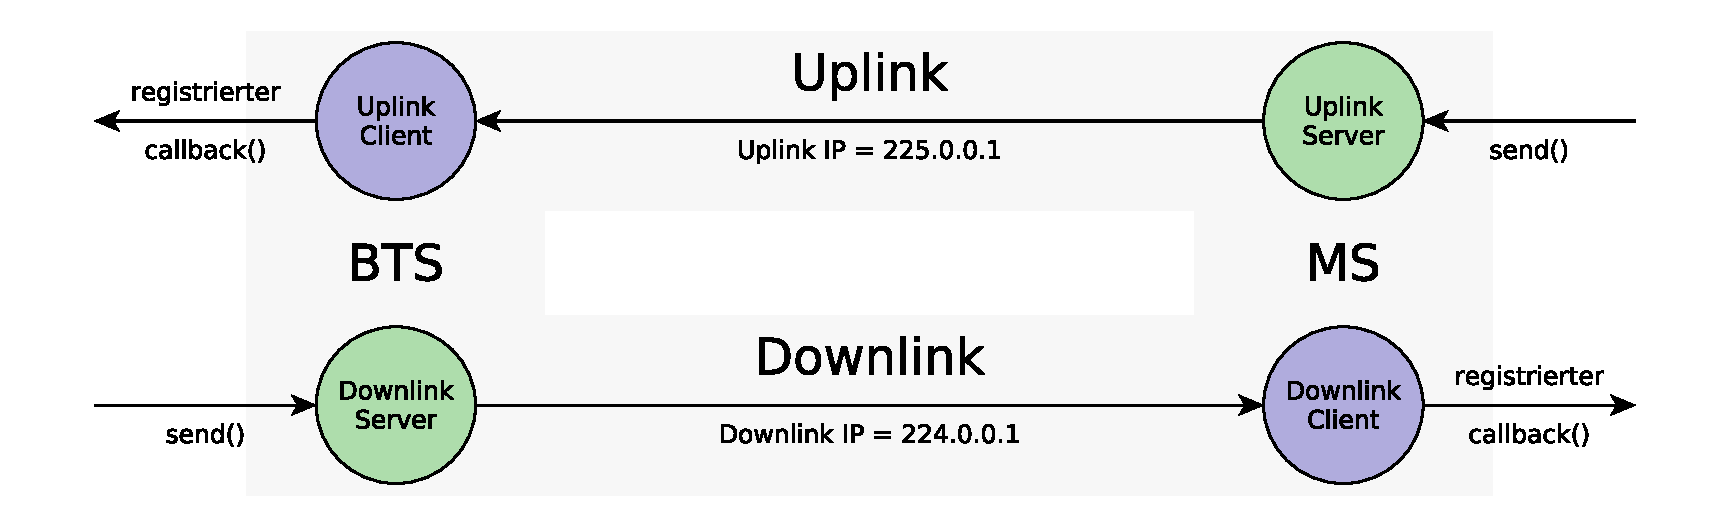
\includegraphics[width=0.9\textwidth]{figures/virt_um_with_multicast.pdf}
	\caption[Die Umsetzung der virtuellen Funkschnittstelle mit Multicast-Sockets]{Die Umsetzung der virtuellen Funkschnittstelle mit Multicast-Sockets, erstellt mit yEd} \label{fig:virt-um-with-mcast}
\end{figure}

Wie in \autoref{fig:virt-um-with-mcast} zu sehen, werden dabei je ein Server-Socket und ein Client-Socket zu Uplink und Downlink zusammengeschlossen. Die \ac{MS} kann über die \texttt{send()} Funktion Daten auf dem Uplink senden und über den \texttt{callback()} auf dem Downlink empfangen. Der Callback wird beim Start des virtuellen \ac{Um} registriert und ist die Methode, die vom Betriebssystem bei eingehenden Daten auf dem Socket aufgerufen wird. Umgekehrt dazu empfängt die \ac{BTS} auf dem Uplink und sendet auf dem Downlink. Durch die Realisierung mit Multicast-Sockets, können mehrere \ac{MS} und auch \ac{BTS} am virtuellen \ac{Um} angemeldet werden. Fügt man in \autoref{fig:virt-um-with-mcast} zum Beispiel eine weitere \ac{MS} hinzu und konfiguriert sie mit den selben \ac{IP}-Adressen für Uplink (225.0.0.1) und Downlink (224.0.0.1), werden alle vom \ac{BTS} gesendeten Nachrichten von beiden \ac{MS} empfangen. Für die Virtualisierung wurde in den beiden Osmocom Projekten osmocomBB und osmoBTS die Implementierung der physikalischen Schicht der Funkschnittstelle ersetzt. Da auf der Socket-Ebene die Anforderungen des virtuellen \ac{Um} auf \ac{MS} und \ac{BTS}-Seite die selben sind, wurde die damit zusammenhängende Funktionalität gekapselt. Die Datei \texttt{virt\_um.c} wird auf beiden Seiten als geteilte Ressource verwendet, automatisiert die Erstellung der Sockets, lässt sich mit Uplink und Downlink-Adressen sowie der \texttt{callback()} Methode konfigurieren und bietet die \texttt{send()} Funktion an.

Mit der Einbindung des virtuellen \ac{Um} in osmocomBB, osmoBTS und osmoMITM konnte der \ac{MitM}-Angriff erfolgreich simuliert und verifiziert werden. Auf der OsmoDevCon2017\footnote{\url{https://osmocom.org/projects/osmo-dev-con/wiki/OsmoDevCon2017}} wurde die Möglichkeit angesprochen, das virtuelle \ac{Um} in Zukunft in das Projekt osmoTester einzubinden. Da dadurch schnelle, hardwareunabhängige Tests möglich sind, kann es von Jenkins \footnote{\url{https://jenkins.io/}} zur Überprüfung korrekter Nachrichtenabläufe auf der Funkschnittstelle bei neuen Commits verwendet werden. Jenkins ist ein webbasiertes Tool für die Automatisierung des Software-Building Prozesses und wird dafür in Osmocom verwendet.

\section{OsmoBTS mit virtueller Um-Schnittstelle}

Das osmoBTS Projekt unterstützt unterschiedliche Hardware, was sich in der Ordnerstruktur widerspiegelt. So ist ein Großteil der \ac{BTS}-Funktionalität in einem Ordner \texttt{src/common}, der gemeinsam genutzte Funktionalität beinhaltet, ausgelagert. Er enthält vor allem die Implementierungen der hardwareunabhängigen, höheren Protokollschichten. Die Schnittstellen für die Unterstützung unterschiedlicher Transceiverhardware sind in mehreren weiteren Ordnern zu finden. Im Ordner \texttt{src/osmo-bts-trx} liegt zum Beispiel Code der Bursts auf einer \ac{UDP}-Schnittstelle von verschiedenen \ac{SDR}-Geräten entgegennimmt und verarbeitet. In \texttt{src/osmo-bts-sysmo} liegt eine Implementierung der physikalischen Schicht, mit der von sysmocom hergestellte \ac{BTS} Produkte über Ethernet angebunden werden können. Der Automake\footnote{\url{https://www.gnu.org/software/automake/manual}} Build-Prozess verbindet die Implementierungen der Protokollschichten und baut für jede der unterstützen Hardwaregeräte eine eigene Anwendung zusammen.

Für osmoBTS wurde in dieser Arbeit im Ordner \texttt{src/osmo-bts-virtual} die physikalische Schicht zur Unterstützung der virtuellen \ac{Um}-Schnittstelle implementiert. Sie erwartet und verarbeitet in \ac{GSMTAP} verpackte Nachrichten auf einem Multicast-Socket. Folgende Grafik zeigt die Schnittstellen der virtuellen \ac{BTS} (\texttt{osmo-bts-virt}) im Vergleich zu den anderen erwähnten \ac{BTS}-Anwendungen \texttt{osmo-bts-trx} und \texttt{osmo-bts-sysmo}.

\begin{figure}[H]
	\centering 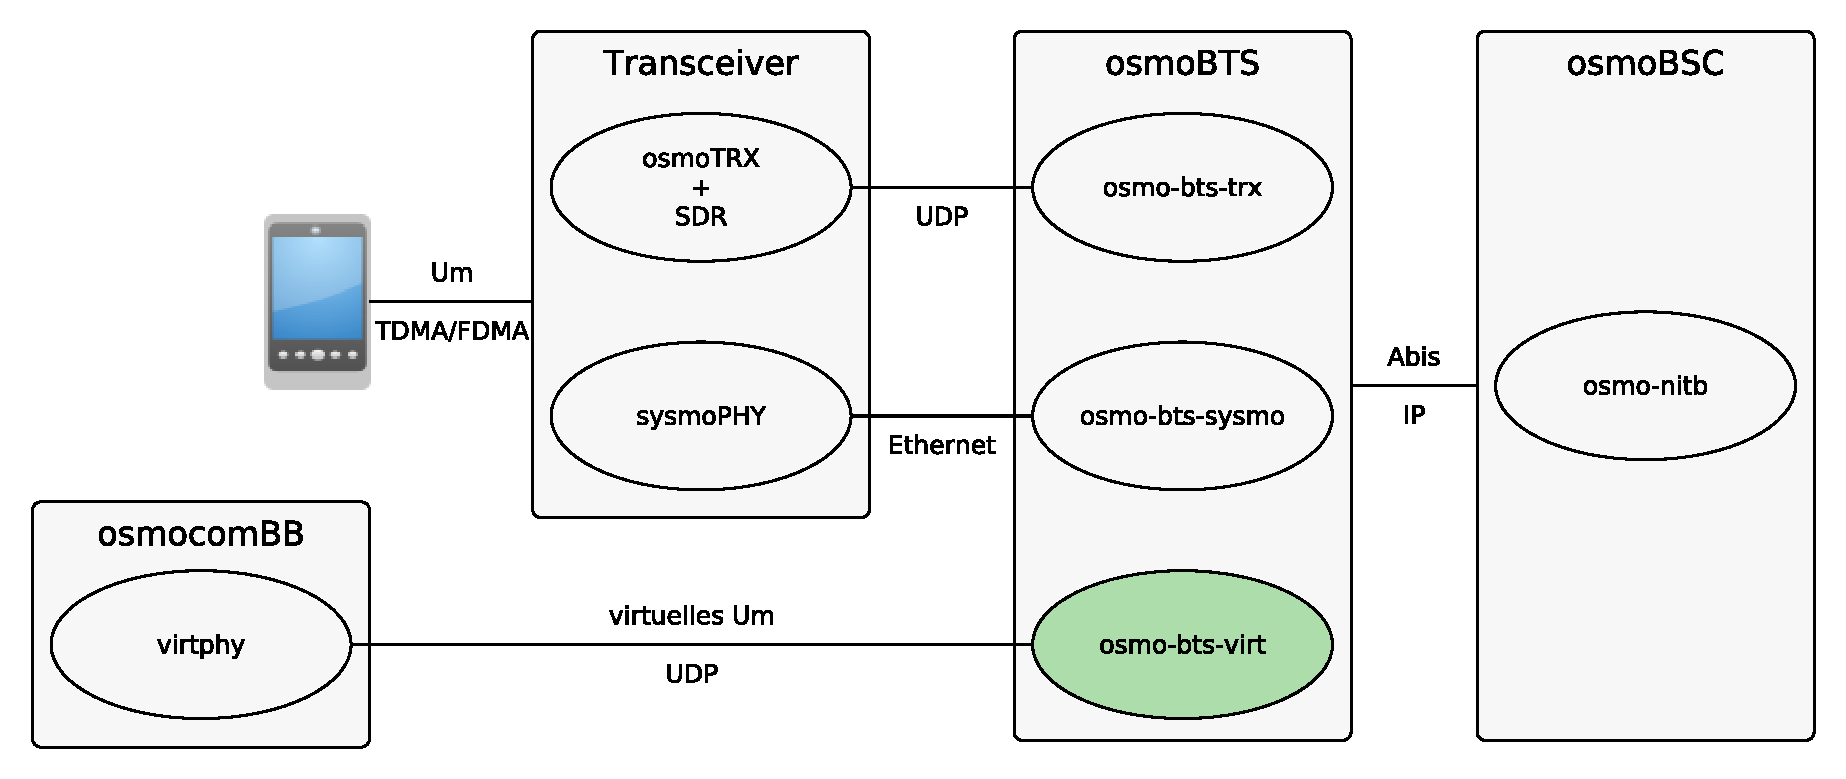
\includegraphics[width=1.0\linewidth]{figures/virt-bts-in-osmocom.pdf}
	\caption[Die Integration der virtuellen physikalischen Schicht in osmoBTS]{Die Integration der virtuellen physikalischen Schicht in osmoBTS, erstellt mit yEd} \label{fig:virt-bts-in-osmocom}
\end{figure}

Wie in obiger Grafik zu sehen, kann die virtuelle \ac{BTS} direkt über das virtuelle \ac{Um} mit verbundenen Mobiltelefonen kommunizieren und braucht keine Schnittstelle zu Transceiverhardware, wie \texttt{osmo-bts-trx} und \texttt{osmo-bts-sysmo}. Die Abis-Schnittstelle zum \ac{BSC} genauso wie die Protokollschichten 2 und 3 sind im \texttt{common} Teil des osmoBTS Projekts implementiert und werden aus diesem eingebunden. In der virtuellen Testumgebung wurde in dieser Arbeit \texttt{osmo-nitb} als \ac{BSC} verwendet (siehe \autoref{hdl:grundlagen_osmocom_OpenBSC}). Neben der Funktion als \ac{BSC} enthält \texttt{osmo-nitb} weitere Funktionalität von Komponenten des \ac{SS7} Netzwerks, wie zum Beispiel dem \ac{HLR}. Bei der Implementierung der physikalischen Schicht von \texttt{osmo-bts-virt} wurden folgende Aufgaben gelöst:
\begin{description}
\item[Build-Prozess] Das neue Programm wurde in den Automake Build-Prozess von osmoBTS eingebunden.
\item[Implementierung des \ac{SAP} der physikalischen Schicht zu höheren Schichten.] Die in \texttt{src/common} implementierten Protokolle \ac{LAPDm} und \ac{RR}, rufen verschiedene \ac{SAP}"=Rou\-tinen der physikalischen Schicht auf (siehe \autoref{hdl:sap}). Sie erwarten vom \ac{SAP} die korrekte Bestätigung (\ac{CON}-Primitives) ihrer Anfragen (\ac{REQ}-Primitives) und den Versand einiger \ac{IND}-Primitives von der physikalischen Schicht. Da andernfalls die höheren Schichten nicht korrekt arbeiten, wurde in der physikalischen Schicht die vollständige \ac{SAP}-Schnittstelle implementiert. Die Funktionalität der \ac{SAP}-Routinen wurde an das virtuelle \ac{Um} angepasst. Die Routine zur Übertragung einer Nutz- oder Signalisierungsnachricht verpackt diese zum Beispiel in \ac{GSMTAP} und schickt sie mit der \texttt{send()} Funktion von \texttt{virt\_um.c} an die konfigurierte Multicast-Adresse. Um die \ac{RR}-Schicht regelmäßig mit der aktuellen \ac{GSM}-Zeit zu versorgen, wurde ein alle 4.615 ms (Dauer eines Frames, siehe \autoref{hdl:a_tdma_fdma}) wiederkehrender Timerinterrupt definiert. Die Interrupt-Routine signalisiert der \ac{RR}-Schicht mit einem \ac{IND}-Primitive den Anfang eines neuen Frames. Die Funktionalität einiger \ac{SAP}-Routinen wird im virtuellen \ac{Um} nicht simuliert und wurde deshalb nicht implementiert. Dazu gehören zum Beispiel "`Frequency Hopping"', die Anpassung der Stärke des gesendeten Signals und die Verschlüsselung von \ac{RR}-Verbindungen.
\item[Parsen der eingehenden \ac{GSMTAP}-Nachrichten.] Da die Verwendung von \ac{GSMTAP} zur Nachrichtenübertragung innerhalb von Osmocom Programmen neu ist, fehlte die Logik zum Auslesen der Informationen des Headers. Diese wurde implementiert.
\item[Multiframe und \ac{TDMA}-Scheduling.] Damit ausgehende Nachrichten auf dem richtigen physikalischen und logischen Kanal gesendet werden, ist ein Scheduler notwendig. Es müssen periodische Aufgaben, wie das Broadcasting von \ac{SI}-Nachrichten und einmalige Aufgaben, wie der durch einen \ac{SAP}-Befehl initiierte Versand einer Nachricht, vom Scheduler für eine bestimmte \ac{FN} geplant und ausgeführt werden. In osmoBTS ist eine Kombination aus Multiframe- und \ac{TDMA}-Scheduler implementiert, dessen Basisfunktionalität im \texttt{common}-Teil zu finden ist. Die Funktionalität für die Planung von einmaligen und periodischen Aufgaben konnte übernommen werden. Die Routinen zur Ausführung, also in der Regel dem Versand einer Nachricht auf einem logischen Kanal, wurden neu geschrieben, so dass sie das virtuelle \ac{Um} für die Übertragung nutzen.
\item[Konfiguration der \ac{BTS} über \ac{VTY}.] Um die virtuelle \ac{BTS} über das Terminal konfigurieren zu können, wurde die \ac{VTY}-Schnittstelle implementiert. Die Konfiguration wird im physikalischen Modell der virtuellen \ac{BTS} (ein C-Struct) gespeichert und verschiedenen Routinen durch Shared-Memory zur Verfügung gestellt. Mit \ac{VTY} können zum Beispiel die Multicast-Adressen für Uplink und Downlink konfiguriert werden.
\item[Implementierung von \ac{OML}.] Beim Start meldet sich die \ac{BTS} bei ihrem zuständigen \ac{BSC} und nimmt anschließend auf der Abis Schnittstelle über den \ac{OML} mehrere Konfigurationen von diesem entgegen. So kann der \ac{BSC} zum Beispiel die Transceiverhardware der \ac{BTS} sowie aktive physikalische Kanäle und das zugewiesene Multiframe konfigurieren. Dabei handelt es sich um Konfigurationen auf physikalischer Ebene, die auf dem Hardwaremodell abgebildet werden müssen. Die \ac{OML}-Routinen wurden implementiert und auf dem physikalischen Modell der virtuellen \ac{BTS} abgebildet.
\end{description}

Zu Beginn der Arbeit war bereits die Implementierung eines Gerüsts für die virtuelle \ac{BTS} vorhanden. Das Gerüst umfasste die Einbindung und Konfiguration des Schedulers, die teilweise Implementierung der \ac{SAP} und \ac{OML}-Schnittstellen sowie Anpassungen an der \ac{VTY}-Schnittstelle der \ac{BTS}. Diese Implementierung wurde als Grundlage übernommen und erweitert. Sie befindet sich unverändert im Branch \texttt{laforge/virt-phy} des osmoBTS Github Repositories\footnote{\url{https://github.com/osmocom/osmo-bts.git}}. Die neue Implementierung, die mit ihrer Gegenseite im osmocomBB Projekt kompatibel ist, befindet sich im Branch \texttt{stumpf/virt"=phy}. Das Programm kann mit Automake und einem C-Compiler kompiliert und dann mit der ausführbaren Datei \texttt{osmo-bts-virtual} gestartet werden. Die Konfiguration erfolgt entweder über die \ac{VTY}-Konfigurationsschnittstelle, über die im osmoBTS Benutzerhandbuch nachgelesen werden kann, oder direkt über die Konfigurationsdatei im Projektordner. Beispielkonfigurationsdateien sind in \texttt{src/osmo-bts-virtual/example-configs} zu finden.

\section{OsmocomBB mit virtueller Um-Schnittstelle}

OsmocomBB ist eine Sammlung von Software rund um eine \ac{MS}, die in der Regel mit dem Konsolenprogramm Osmocon verwendet wird. Mit Osmocon ist es möglich, die Firmware im flüchtigen Speicher eines der unterstützten Mobiltelefone, wie zum Beispiel dem Motorola C123, auszutauschen. Über eine serielle Schnittstelle kann man das Telefon mit einem Linux Rechner verbinden und von diesem aus steuern, welches der vorkompilierten Firmware Pakete auf das Telefon geladen werden soll. Die einfachste Firmware dürfte \texttt{hello\_world} sein, die auf dem Display des Mobiltelefons einen Text ausgibt. \texttt{rssi\_scan} kann die \acp{RSSI}, also die Signalstärken der \ac{BTS} im Umkreis, messen und stellt diese auf dem Display dar. Die umfangreichste Firmware ist \texttt{layer1}. Sie implementiert die physikalische Schicht des \ac{GSM}-Protokollstapels für den Baseband-Prozessor. Für die Steuerung der Funktionen des Baseband-Prozessors und des \ac{DSP} von außen gibt es eine Kontrollschnittstelle. Diese Schnittstelle wird \ac{L1CTL} genannt und ist ein nicht spezifiziertes, osmocomBB-internes Protokoll. Osmocon bietet für den Zugriff auf die Schnittstelle ein lokales Linux-Domain-Socket an und leitet den Datenverkehr auf diesem über die serielle Schnittstelle zur \texttt{layer1}-Firmware weiter. Der Funktionsumfang des \ac{L1CTL}-Protokolls entspricht im Großen und Ganzen dem \ac{SAP} der physikalischen Schicht, die verschiedenen \ac{L1CTL}-Headertypen den \ac{SAP}-Primitives. Im Gegensatz zu einer internen \ac{SAP}-Schnittstelle ist die externe \ac{L1CTL}-Schnittstelle aber von außen über das Socket zugänglich. Mehrere sogenannte L23-Apps, die die Funktionalität der höheren \ac{GSM}-Protokollschichten implementieren, nutzen \ac{L1CTL} für die Steuerung der physikalischen Schicht des verbundenen Mobiltelefons. Die L23-App \texttt{ccch\_scan} ist ein passiver \ac{CCCH} und \ac{BCCH} Sniffer, der empfangene Nachrichten über \ac{GSMTAP} protokolliert. \texttt{cell\_log} macht einen vollständigen Messdurchlauf der Empfangsstärken aller \ac{ARFCN} und gibt das Ergebnis auf der Kommandozeile aus. Besonders interessant ist die L23-App \texttt{mobile}, die die Funktionalität eines klassischen Mobiltelefons simuliert und über eine \ac{VTY}-Schnittstelle gesteuert werden kann. Damit kann der Nutzer zum Beispiel eine Telefonnummer anrufen, eine \ac{SMS} versenden oder nach \ac{BTS} in Reichweite suchen. 

Die Struktur des Projekts trennt strikt zwischen Host-Software und Target-Software. Im Ordner \texttt{src/host} befinden sich alle Anwendungen, die auf dem Linux-Rechner laufen, wie die L23-Apps und Osmocon. In \texttt{src/target} wird die Software für das Mobiltelefon gesammelt. Sie muss zuerst cross-kompiliert und dann mit Osmocon geladen werden. Das sind alle Firmware- Implementierungen wie \texttt{layer1} oder \texttt{rssi\_scan}. Da die Anwendung für das virtuelle \ac{MS} nicht auf dem Mobiltelefon, sondern auf dem Rechner ausgeführt wird, wurde der Ordner \texttt{virt\_phy} für dessen Entwicklung in \texttt{src/host} angelegt. Folgende Grafik zeigt die Schnittstellen der virtuellen physikalischen Schicht (\texttt{virthphy}) in osmocomBB im Vergleich mit anderen Target- und Host-Anwendungen.

\begin{figure}[H]
	\centering 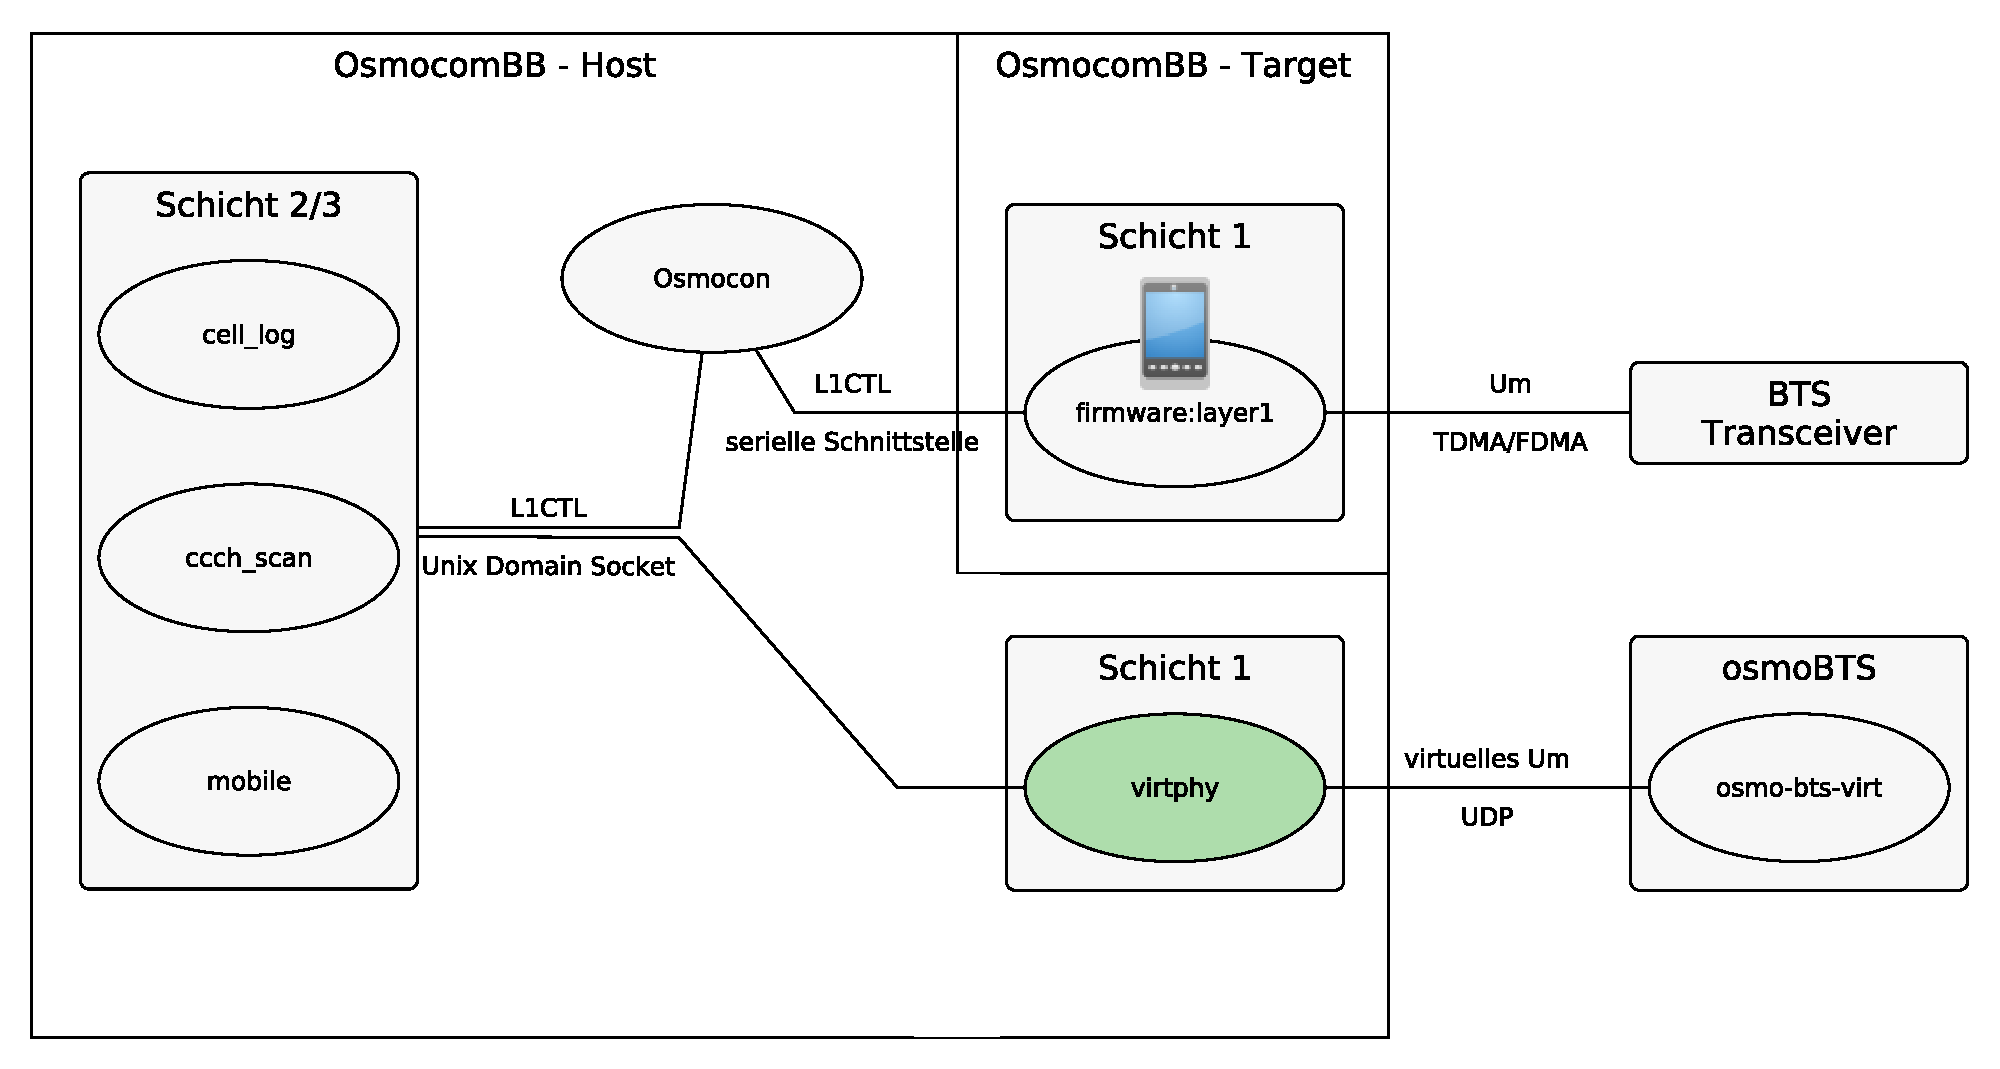
\includegraphics[width=1.0\linewidth]{figures/virt-bb-in-osmocom.pdf}
	\caption[Die Integration der virtuellen physikalischen Schicht in osmocomBB]{Die Integration der virtuellen physikalischen Schicht in osmocomBB, erstellt mit yEd} \label{fig:virt-bb-in-osmocom}
\end{figure}

In \autoref{fig:virt-bb-in-osmocom} kann man erkennen, dass \texttt{virtphy} die strikte Trennung der physikalischen Schicht von den höheren Schichten einhält. \texttt{virtphy} implementiert nur die physikalische Schicht der virtuellen \ac{MS}, die höheren Protokollschichten liegen in den L23-Apps. Die Osmocon Anwendung wurde nicht mit eingebunden, da dessen Hauptfunktionalität, Firmware auf ein Target zu laden, nicht benötigt wird. Neben der Schnittstelle zum virtuellen \ac{Um}, bietet die virtuelle physikalische Schicht also auch die \ac{L1CTL}-Schnittstelle über ein Linux-Domain-Socket an. Der Funktionsumfang von \texttt{virtphy}, das als eigener Prozess auf dem Rechner läuft, entspricht in etwa der \texttt{layer1}-Firmware. Alle Aufgaben die bei der Implementierung der gelöst wurden sind im Folgenden zusammengefasst.
\begin{description}
\item[Build-Prozess.] Die \texttt{virt-phy} Anwendung wurde in den Build-Prozess von osmocomBB eingebunden. Wie in osmoBTS wird Automake verwendet.
\item[Implementierung des \ac{L1CTL}-Sockets] Die Funktionalität zur Erstellung und Konfiguration des \ac{L1CTL}-Sockets wurde aus Osmocon übernommen und in einer eigenen Datei \texttt{l1ctl\_sock} gekapselt.
\item[Parsen von \ac{GSMTAP}.] Die \ac{GSMTAP}-Logik wurde über geteilte Ressourcen aus der virtuellen \ac{BTS} Implementierung eingebunden. 
\item[Implementierung der \ac{L1CTL}-Schnittstelle.] Um das \ac{L1CTL}-Protokoll implementieren zu können wurde die Kommunikation zwischen der \texttt{layer1}-Firmware und verschiedenen L23-Apps analysiert. Von der L1CTL-Schnittstelle gibt es keine offizielle Dokumentation. Die Aufgaben der verschiedenen \ac{L1CTL}-Routinen wurden durch Debugging und Codeanalyse, sowie teilweise Dokumentation im Code herausgefunden, was deren Implementierung in der virtuellen physikalischen Schicht ermöglichte. Das \ac{L1CTL}-Protokoll orientiert sich dabei stark am \ac{SAP} der physikalischen Schicht und definiert verschiedene \ac{REQ}, \ac{IND} und \ac{CON}-Nachrichtentypen (siehe \autoref{hdl:sap}). Um Fehler in den L23-Apps zu vermeiden, wurde die Schnittstelle vollständig implementiert und die ausgeführten \ac{L1CTL}-Routinen an das virtuelle \ac{Um} angepasst. Unter anderem wurde die Funktionalität der Routinen zur Messungen von Signalstärken, Senden einer Signalisierungsnachricht, dem Wechsel in den dedizierten Modus und der Synchronisation mit einer \ac{BTS} implementiert. Alle Nachrichten des \ac{L1CTL}-Protokolls sind mit einer kurzen Beschreibung und dem Status der zugehörigen Routine in der Implementierung der virtuellen physikalischen Schicht, in \autoref{hdl:a_l1ctl-routines} hinterlegt.
\item[Routine zur Messung von Signalstärken.] Auf dem virtuellen \ac{Um} gibt es keine unterschiedlichen Signalstärken. Alle Nachrichten auf dem Multicast-Socket werden mit gleicher Qualität empfangen. Da die \ac{MS} sich jedoch immer mit der \ac{BTS} mit dem besten Empfang verbindet, ist die Simulation der Signalstärken wichtig. Durch die Konfiguration unterschiedlicher Signalstärken für verschiedene \acp{BTS}, kann Einfluss darauf genommen werden, mit welcher \ac{BTS} sich das \ac{MS} verbindet. Die Messung von Signalstärken wird über die \ac{L1CTL}-Nachricht \texttt{L1CTL\_PM\_REQ} von der L23-App, für eine Liste von \acp{ARFCN}, gestartet. Die in der Antwort \texttt{L1CTL\_PM\_CON} zurückgegebenen Messwerte der virtuellen physikalischen Schicht wurden so definiert: \acp{ARFCN} von denen regelmäßig eine Nachricht auf dem virtuellen \ac{Um} empfangen wird, erhalten die maximale Signalstärke (> -63 dBm in \ac{GSM}), alle anderen die minimale Signalstärke (< -110 dBm in \ac{GSM}). Damit wird gewährleistet, dass die \ac{RR}-Schicht nur die Verbindung mit verfügbaren \ac{ARFCN} initiiert. Des Weiteren kann mit Kommandozeilenparametern von \texttt{virtphy}, für jede \ac{ARFCN} ein Signalstärkereduktionswert angegeben werden, um den der zurückgegebene Signalstärkemesswert dieser \ac{ARFCN} reduziert wird. Damit kann der Anwender unterschiedlichen Empfang für die \ac{BTS} auf dem virtuellen \ac{Um} konfigurieren und so beeinflussen, mit welcher \ac{BTS} sich das \ac{MS} verbindet.
\item[Routine zur Synchronisation der \ac{MS} mit einer \ac{BTS}.] Die \ac{RR}-Schicht in der L23-App schickt die \ac{L1CTL}-Nachricht \texttt{L1CTL\_FBSB\_REQ}, um sich mit einer ausgewählten \ac{ARFCN} zu verbinden, sobald ihr die Signalstärkemesswerte aller \acp{ARFCN} vorliegen. Im Gegensatz zur realen Funkschnittstelle ist auf dem virtuellen \ac{Um} keine Frequenzsynchronisation nötig, da auf dem Multicast-Socket die Nachrichten aller \ac{BTS} empfangen werden. Auf dem virtuellen \ac{Um} senden die \acp{BTS} außerdem keine Nachrichten auf dem \ac{SCH}, der für die zeitliche Synchronisation mit dem Multiframe verwendet wird. Die Synchronisationsmechanismen wurden deshalb wie folgt an das virtuelle \ac{Um} angepasst. Die Synchronisation mit einer \ac{ARFCN} wird durch das Herausfiltern aller Nachrichten von anderen \acp{ARFCN} erreicht. Die zeitliche Synchronisation ist auf der realen Funkschnittstelle nötig, um die empfangenen Nachrichten den korrekten logischen und physikalischen Kanälen zuordnen zu können. Auf dem virtuellen \ac{Um} sind die Informationen, die für die Zuordnung benötigt werden (\ac{FN} und \ac{TDMA}-Zeitschlitz), im \ac{GSMTAP}-Header jeder Nachricht verfügbar. Insofern wird die zeitliche Synchronisation dafür nicht benötigt. Der Scheduler muss für die Planung von Aufgaben für eine \ac{FN} in der Zukunft aber die aktuelle \ac{FN} kennen. Um dem Scheduler diese Information zu Verfügung zu stellen, aktualisiert die virtuelle physikalische Schicht, mit jeder eingehenden Nachricht von der synchronisierten \ac{BTS}, eine lokale \ac{FN} im Modell der virtuellen \ac{MS}. Diese wird dem Scheduler zur Verfügung gestellt.
\item[Scheduling.] Die Implementierung des Schedulers besteht aus der Planungslogik, die Aufgaben für den richtigen physikalischen und logischen Kanal einplant und der Ausführungslogik der Aufgaben. Der Scheduler wird, sobald die \ac{MS} mit einer \ac{BTS} verbunden ist, bei jeder auf dem virtuellen \ac{Um} empfangenen Nachricht ausgeführt. Der Scheduler ist damit nicht aktiv zeitgesteuert, sondern passiv und abhängig von eingehenden Nachrichten. Da das \ac{MS} von der \ac{BTS} jedoch regelmäßig Nachrichten auf dem \ac{BCCH} und anderen Kanälen erhält, ist diese einfache und passive Lösung ausreichend. Der Scheduler wird mit dieser Lösung nicht für jede \ac{FN} aufgerufen und führt deshalb der Reihe nach alle Aufgaben aus, die für die aktuelle und kleinere \ac{FN} geplant wurden. Für den Scheduler wurde bewusst eine einfache Variante gewählt. In den aufgezeichneten Mitschnitten konnte die Lösung die richtige Reihenfolge und \ac{FN} der gesendeten Nachrichten gewährleisten und war somit ausreichend.
\item[Schnittstelle zum \ac{SIM}.] Für die Ausführung der Sicherheitsalgorithmen benötigt die \ac{MS} eine Schnittstelle zum \ac{SIM}. In der \texttt{layer1}-Firmware ist diese implementiert und wird über eine \ac{L1CTL}-Routine für höhere Schichten zur Verfügung gestellt. Auch das virtuelle \ac{MS} braucht Zugriff auf Daten und Sicherheitsalgorithmen der \ac{SIM}-Karte. Dazu kann entweder das \ac{SIM} simuliert, oder die Schnittstelle zu einem \ac{SIM}-Kartenlesegerät implementiert werden. In der L23-App \texttt{mobile} kann eine \texttt{test-sim} Option aktiviert werden, mit der sie eine \ac{SIM}-Karte simuliert und zur Verfügung stellt. Die \ac{L1CTL}-Routine für den Zugriff auf die \ac{SIM}-Karte wurde deshalb nicht implementiert, sondern stattdessen die Aktivierung der \texttt{test-sim} Option vorausgesetzt. Damit ein virtuelles \ac{MS} Zugriff auf alle Netzwerkdienste hat, muss die \ac{SIM}-Karte einen gültigen Netzteilnehmer identifizieren. Dazu muss die auf der Test-\ac{SIM} gespeicherte \ac{IMSI} auch im \ac{HLR} vorhanden sein. In osmoNITB ist das \ac{HLR} durch eine SQLite-Datenbank realisiert, in die die Werte der Netzteilnehmer eingetragen werden.
\end{description}

Einige Funktionen der \ac{Um}-Schnittstelle werden aktuell (Stand Mai 2017) noch nicht von den Implementierungen für das virtuelle \ac{MS} und \ac{BTS} unterstützt. Dazu gehören Frequency Hopping, Sprachdatenübertragung, sowie Kodierung und Verschlüsselung des Nachrichtenverkehrs. Für die praktische Durchführung des \ac{MitM}-Angriffs war die Implementierung dieser Funktionen nicht notwendig. Für die virtuelle physikalische Schicht gibt es zudem keine \ac{VTY} Konfigurationsschnittstelle. Die Konfiguration erfolgt über Kommandozeilenparameter beim Start des Programms.

\section{Die Validierung der Manipulation der Setup-Nachricht mit Testdaten}\label{hdl:coder-impl}

Wegen der fehlenden Kanalkodierung und Verschlüsselung auf dem virtuellen \ac{Um} wurden das Kommandozeilenprogramm \texttt{dummycoder} und das Python Skript \texttt{xor\_hexstrings} geschrieben. Beide Programme befinden sich im osmoMITM\footnote{\url{https://github.com/BastusIII/osmo-mitm.git}} Repository.

Die Kodierungsfunktionalität wurde in \texttt{coder.c} implementiert. Für die Kodierung und Dekodierung einer Nachricht auf dem  \ac{FACCH} wurden die Funktionen \texttt{facch\_encode()} und \texttt{facch\_decode()} geschrieben, für alle anderen Signalisierungskanäle \texttt{xcch\_encode()} und \texttt{xcch\_decode()}. Die Funktionen nehmen als Eingangsdaten das beliebige Ergebnis eines Zwischenschrittes der Kanalkodierung entgegen und geben die Zwischenergebnisse aller angewendeten Kodierungsfunktionen zurück. Der Grund für die Trennung von \ac{FACCH} von anderen Signalisierungskanälen liegt in den unterschiedlichen kombinierten Kodierungsverfahren (siehe \autoref{hdl:encoding}). Die Kodierungsverfahren für Firecode und Faltungskodierung werden von der libosmocore Bibliothek zur Verfügung gestellt und wurden aus dieser verwendet. Die Logik für Interleaving und Burstmapping wird nicht von der Bibliothek angeboten, konnte aber aus \texttt{osmo-bts-trx} übernommen werden.

Das Programm \texttt{dummycoder} liest Hexstrings aus Textdateien ein, kodiert oder dekodiert sie auf Wunsch des Anwenders und speichert das Ergebnis wieder ab. Dafür verwendet es die von \texttt{coder.c} bereitgestellten Funktionen und enthält selbst nur die Logik zum Einlesen und Formatieren der Eingangs- und Ergebnisdaten. Das Python Skript \texttt{xor\_hexstrings} ließt zwei Hexstrings ein und verknüpft diese mit der \ac{XOR}-Operation. Dadurch lässt sich die Stromverschlüsselung einer \ac{GSM}-Nachricht simulieren.

Im Ordner \texttt{tests} befinden sich zwei Testfälle, in denen die beiden Programme verwendet werden, um eine Beispiel Setup-Nachricht zu kodieren und zu manipulieren. Die Ergebnisse aus \texttt{tests/encode\_decode\_test} sind in die Beispieldaten der Kanalkodierung in \autoref{hdl:encoding} eingeflossen. Das Skript in \texttt{tests/setup\_manip\_test} wurde verwendet, um die Manipulation der Telefonnummer in einer Setup-Nachricht anhand von Beispieldaten zu validieren. Die Konsolenausgabe des Tests ist in \autoref{hdl:a_example_setup_manip} zu finden.

\section{Die Validierung des Angriffs mit einem Man-in-the-Middle im virtuellen Um}\label{hdl:mitm_impl}

Für die praktische Nachstellung des in \autoref{hdl:theroetical-attack} ausgearbeiteten Angriffs wurde ein \ac{MitM} auf dem virtuellen \ac{Um} implementiert. Der \ac{MitM} hat Zugriff auf den Uplink und Downlink des virtuellen und eines korrumpierten \ac{Um} und stellt die Verbindung zwischen beiden her. Alle \ac{MS} die sich mit dem korrumpierten virtuellen \ac{Um} verbinden, kommunizieren so über den \ac{MitM} mit dem Netzwerk und der \ac{MitM} hat Zugriff auf den kompletten Datenverkehr. Die Implementierung besteht aus einem Rahmen, der die Funktionalität der zwei virtuellen \ac{Um}-Schnittstellen anbietet, und einer Verarbeitungslogik. Die Verarbeitungslogik wird über zwei als extern deklarierte Callbackfunktionen eingebunden. Der Uplink-Callback wird bei einer eingehenden Nachricht auf dem korrumpierten Uplink aufgerufen, sein Rückgabewert an das \ac{Um} weitergeleitet. Der Downlink-Callback wird bei einer eingehenden Nachricht auf dem Downlink aufgerufen, sein Rückgabewert an das korrumpierte \ac{Um} weitergeleitet. Ein Rückgabewert von NULL bedeutet, dass die Nachricht blockiert wurde. Damit können Nachrichten von der Verarbeitungslogik verändert, verzögert oder abgefangen werden. \autoref{fig:virtual-um-mitm} zeigt, wie die \ac{MitM}-Verarbeitungsroutinen im \ac{MitM}-Gerüst eingebunden sind und die Vermittlung von Nachrichten zwischen virtuellen \ac{Um} und korrumpiertem virtuellen \ac{Um}.

\begin{figure}[H]
	\centering 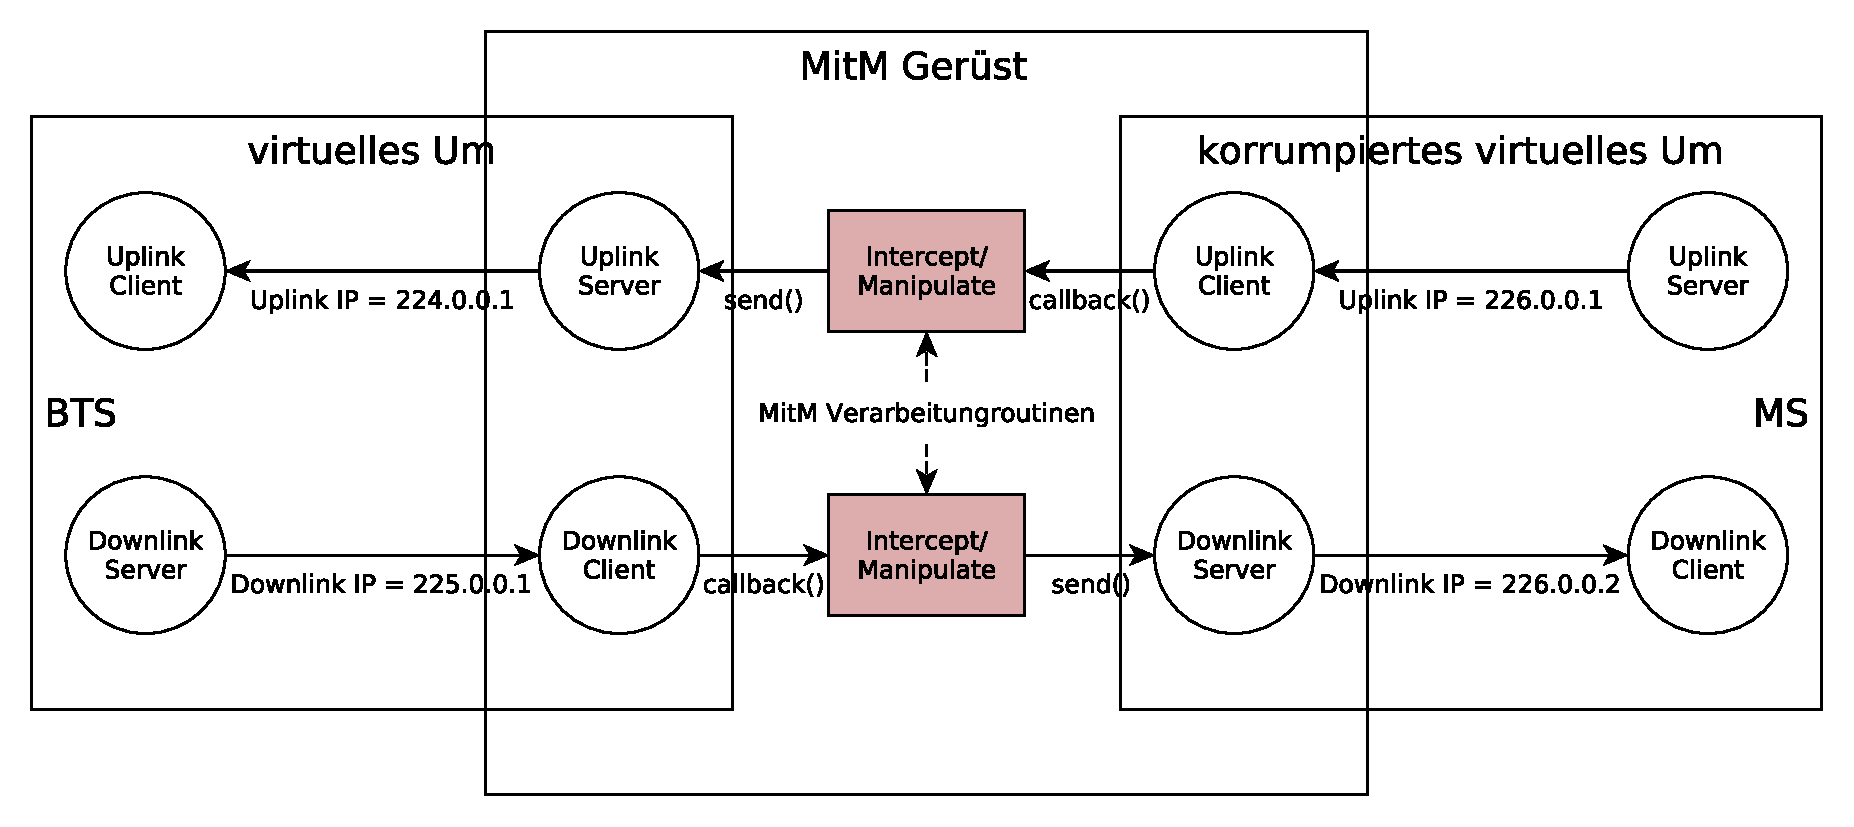
\includegraphics[width=1.0\textwidth]{figures/mitm_in_virt_um_with_multicast.pdf}
	\caption[Die MitM-Implementierung im virtuellen Um]{Die \ac{MitM}-Implementierung im virtuellen \ac{Um}, erstellt mit yEd} \label{fig:virtual-um-mitm}
\end{figure}

Das \ac{MitM}-Gerüst muss über Kommandozeilenparameter mit den \ac{IP}-Adressen von Uplink und Downlink des \ac{Um} und des korrumpierten \ac{Um} konfiguriert werden, da es die Logik für den Aufbau der virtuellen \ac{Um}-Schnittstellen enthält. Von den Verarbeitungsroutinen benötigte, zusätzliche Optionen können über einen Optionshandler definiert werden. Eine Verarbeitungsroutine muss neben dem Optionshandler nur die beiden Funktionen implementieren die empfangene Nachrichten analysieren und bearbeiten. Sie kann deshalb leicht ausgetauscht werden. Im Zuge der Masterarbeit wurden drei Verarbeitungslogiken entwickelt. \texttt{SimpleForward} leitet alle Nachrichten, ohne sie zu verändern, sobald sie eingehen, sofort weiter. \texttt{ImsiCatcher} realisiert einen \ac{IMSI}-Catcher, der eine \ac{GSM} Schwachstelle ausnutzt, um die aktuellen \acp{TMSI} der Netzteilnehmer ihren \acp{IMSI} zuzuordnen und damit ihre Identität offenlegt. \texttt{CallSetupManipulation} kombiniert die Funktionalität des \ac{IMSI}-Catchers mit der im Zuge der Masterarbeit ausgearbeiteten Identifikation und Manipulation der Setup-Nachricht (siehe \autoref{hdl:theroetical-attack}), um ein ausgehendes Telefonat umzuleiten. Die einfachste Routine ist in folgendem Codebeispiel zu sehen. Das C-Struct \texttt{msgb} wird innerhalb von Osmocom verwendet, um eine Nachricht mit Nutzdaten und mehreren Headern zu definieren.\\

%\begin{adjustbox}{max width={0.95\textwidth}, padding=20pt 10pt 10pt 10pt, frame, center}
\begin{lstlisting}[caption={[Die Simple-Forward Verarbeitungsroutine des MitM]Die Simple-Forward Verarbeitungsroutine des \ac{MitM}}, label={lst:simple_forward}, boxpos=c, frame=single, style=CStyle, numbers=none]
#include <osmocom/core/msgb.h>

/**
 * Simple Forward hat keine zusätzlichen Optionen.
 */
void handle_suboptions(int argc, char **argv)
{
	return;
}
/**
 * Rückgabe und damit einfache Weiterleitung der originalen Nachricht.
 */
struct msgb* downlink_rcv_cb_handler(struct msgb *msg) {
	return msg;
}
/**
 * Rückgabe und damit einfache Weiterleitung der originalen Nachricht.
 */
struct msgb* uplink_rcv_cb_handler(struct msgb *msg) {
	return msg;
}
\end{lstlisting}
%\end{adjustbox}

Die Implementierung des \ac{MitM} Frameworks auf dem virtuellen \ac{Um} mitsamt den Verarbeitungsroutinen ist im osmoMITM\footnote{\url{https://github.com/BastusIII/osmo-mitm.git}} Repository hinterlegt.

\subsection{Die Verarbeitungsroutine des IMSI-Catchers}

Die Identitäten auf dem \ac{Um} werden durch die Verwendung einer temporären ID, der \ac{TMSI}, verschleiert. Der Angreifer im vorgestellten \ac{MitM}-Angriff möchte nur die ausgehenden Anrufe von einem bestimmten Netzteilnehmer umleiten. Damit dieser eindeutig vom Angreifer identifiziert werden kann, wird die aktuelle \ac{TMSI} benötigt, die ihm vom Netzwerk zugewiesen wurde. Da die Zuweisung der \ac{TMSI} im "`Location Updating Accept"' oder "`TMSI Reallocation Command"' verschlüsselt geschieht, kann sie nicht aus dem Datenverkehr auf dem \ac{Um} ausgelesen werden. Ein sogenannter \ac{IMSI}-Catcher nutzt Schwachstellen im \ac{GSM}-Standard aus, um die Identitäten verbundener Netzteilnehmer zu sammeln. Da der Angriff die Kenntnis der Identität des Opfers voraussetzt, wurde das \ac{MitM}-Gerüst im virtuellen \ac{Um} um die Logik eines \ac{IMSI}-Catchers erweitert.

Die Grundlage des \ac{IMSI}-Catchers ist eine falsche \ac{BTS}, die auf alle eingehenden Anfragen von verbundenen \ac{MS} mit einem "`Identity Request"' die \ac{IMSI} des \ac{MS} abfragt, diese sammelt und einem Angreifer zur Verfügung stellt. Der \ac{GSM}-Standard spezifiziert, dass eine \ac{MS} während einer \ac{RR}-Verbindung eingehende Identity-Requests immer erwarten und beantworten muss \citepauthor[Kap. 4.3.3.2]{3gpp:24.008}. Da der Identity-Request des Angreifers erfolgt, bevor die Verschlüsselung aktiviert wird, muss er sich darum nicht kümmern.

Hat ein Angreifer Zugriff auf den Datenverkehr auf dem \ac{Um} gibt es zudem mehrere Möglichkeiten, den IMSI-Catcher so zu erweitern, dass er die temporäre Identität (\ac{TMSI}) von Netzteilnehmern auf dem \ac{Um} ihrer eindeutigen Identität (\ac{IMSI}, \ac{MSISDN}) zuordnen kann. Überwacht der Angreifer mit einem passiven Sniffer den \ac{PCH} einer \ac{BTS}, kann er die von einer sogenannten "`Silent \ac{SMS}"' an die \ac{MSISDN} des Opfers ausgelösten Paging Nachrichten analysieren. In einer Paging Nachricht steht in der Regel die \ac{TMSI} des Opfers \citepauthor[Kap. 3.3.2.1.1]{3gpp:04.18}, die der Angreifer so dessen \ac{MSISDN} zuordnen kann. Dem Opfer wird der Empfang einer Silent \ac{SMS} nicht angezeigt, er hat also keine Möglichkeit, den Angriff zu bemerken.

Der in dieser Arbeit implementierte \ac{IMSI}-Catcher setzt einen aktiven Eingriff in den Datenverkehr auf dem \ac{Um} voraus. Der von der \ac{IMSI}-Catcher Verarbeitungsroutine manipulierte Nachrichtenfluss ist in \autoref{fig:mitm-imsi-catcher} dargestellt.

\begin{figure}[H]
	\centering \includegraphics[width=1.0\linewidth]{figures/mscgen/gsm_imsi_catcher.pdf}
	\caption[Die IMSI-Catcher Verarbeitungsroutine des MitM]{Die \ac{IMSI}-Catcher Verarbeitungsroutine des \ac{MitM}, verifiziert mit Wireshark-Mitschnitt auf virtuellem \ac{Um}, siehe \autoref{lst:mitm_attack_wireshark}} \label{fig:mitm-imsi-catcher}
\end{figure}

Die Identität des \ac{MS} wird in der \ac{SABM}-Anfrage (siehe \autoref{fig:mitm-imsi-catcher}, Teil 1) an das Netzwerk entweder als \ac{IMSI} oder als \ac{TMSI} angehängt. Ist die angehängte \ac{TMSI} in einer Anfrage unbekannt, so wird die Nachricht vom Angreifer mit einem Identity-Request beantwortet, der die zugehörige \ac{IMSI} vom \ac{MS} abfragt. Die Identity Response mit der \ac{IMSI} vom \ac{MS} wird abgefangen und die Zuordnung der \ac{IMSI} zur \ac{TMSI} in einer Datenstruktur abgespeichert (siehe Teil 2). Anschließend wird die \ac{RR}-Verbindung mit einem Channel Release vom \ac{MitM} beendet (siehe Teil 3). Das \ac{MS} sendet und empfängt nach dem \ac{DISC} keine weiteren Nachrichten mehr auf dieser Verbindung. Da das Netzwerk vom Release nichts mitbekommt, horcht es noch eine Weile auf der \ac{RR}-Verbindung, wird aber, nachdem es eine bestimmte Zeit keine Nachrichten vom \ac{MS} erhalten hat, von einem Fehler ausgehen und die Verbindung ebenfalls beenden. Da die blockierten Anfragen, wie der Location Update-Request, in der Regel automatisch vom \ac{MS} generiert werden, bemerkt der Nutzer den Angriff nicht.

Der \ac{IMSI}-Catcher auf dem virtuellen \ac{Um} ist wie ein Zustandsautomat aufgebaut. Jeder Nachricht, die als nächstes erwartet wird, wurde ein Zustand zugewiesen. Die beim Zustandsübergang ausgeführten Funktionen definieren, ob und wie die eingegangene Nachricht verändert wird. Mit dem \ac{IMSI}-Catcher wurden Wireshark Mitschnitte mit erfolgreichen Zuordnungen von \ac{TMSI} zu \ac{IMSI} auf dem virtuellen \ac{Um} erstellt (siehe \autoref{lst:mitm_attack_wireshark}). 

\subsection{Die Verarbeitungsroutine der Setup Manipulation}
Die in \autoref{hdl:theroetical-attack} beschriebe Logik für die Manipulation der kodierten und verschlüsselten Setup-Nachricht wurde in dieser Verarbeitungsroutine für den \ac{MitM} auf dem virtuellen \ac{Um} implementiert. Das Ziel ist die Umleitung des Anrufs, indem die angerufene Telefonnummer ausgetauscht wird.

Die Funktionalität der Implementierung umfasst die Identifikation des Opfers, wofür die Logik der oben beschriebenen \ac{IMSI}-Catcher Verarbeitungsroutine eingebunden wurde. Des Weiteren wird die Datenübertragung auf vom identifizierten Opfer ausgehende Anrufe analysiert. Wie die dafür zuständige Setup-Nachricht im Nachrichtenfluss erkannt werden kann, wurde in \autoref{hdl:call-setup-message-flow-analysis} herausgearbeitet. Als Letztes ist die Manipulation der Setup-Nachricht implementiert. Die dafür zuständige Funktion erwartet die \ac{LAPDm}-Nachricht verschlüsselt und kanalkodiert, wofür die Funktionalität des Coders eingebunden wurde (siehe \autoref{hdl:coder-impl}). Das Programm wird über Kommandozeilenparameter mit den als bekannt vorausgesetzten Werten initialisiert und erwartet beim Start deshalb die Telefonnummer des angerufenen Opfers (\texttt{msisdn-called}), die \ac{IMSI} des anrufenden Opfers (\texttt{imsi-victim}) und das Offset der Telefonnummer in der Call Setup-Nachricht (\texttt{msisdn-to-setup-offset}). In folgendem Codebeispiel kann man erkennen, dass die Funktion \texttt{manip\_setup\_msg()}, in der die Manipulation der Setup-Nachricht stattfindet, mit kodierten Daten aufgerufen wird. Die Kodierung übernimmt die \texttt{xcch\_encode()} Funktion aus dem Coder. Die Daten werden nicht verschlüsselt, was ein zusätzliches \ac{XOR} mit einem Schlüsselstrom wäre. Der Nachweis, dass der Angriff mit verschlüsselten Daten funktioniert, ist hier nicht mehr nötig. Er wurde in den Tests in \autoref{hdl:coder-impl} erbracht.\\

%\begin{adjustbox}{max width={0.95\textwidth}, padding=20pt 10pt 10pt 10pt, frame, center}
\begin{lstlisting}[caption={[Die Callbackfunktion für eingehende Nachrichten auf dem Uplink, Auszug aus der Setup-Manipulation Verarbeitungsroutine des MitM]Die Callbackfunktion für eingehende Nachrichten auf dem Uplink, Auszug aus der Setup-Manipulation Verarbeitungsroutine des \ac{MitM}}, label={lst:setup_manip1}, boxpos=c, frame=single, style=CStyle, numbers=none]
// Auszug aus dem Uplink Callback der Setup Manipulation MitM Verarbeitungsroutine.
// msg enthält die empfangene Originalnachricht.
struct msgb* uplink_rcv_cb_handler(struct msgb *msg)
{
	// Extraktion des GSMTAP Headers aus der Nachricht
	struct gsmtap_hdr *gh = msgb_l1(msg);
	// Puffer für manipulierte Nachricht
	struct msgb *manip_msg;
	// Puffer für kodierte Originalnachricht. LEN_BURSTMAP_XCCH ist 4*116.
	uint8_t encoded_msg[LEN_BURSTMAP_XCCH / 8];
	// Puffer für kodierte, manipulierte Nachricht
	uint8_t encoded_manip_msg[LEN_BURSTMAP_XCCH / 8];
	(...)
	switch(mitm_state) {
	(...)
	case STATE_IMSI_CATCHER_SABM:
		// Kopieren des GSMTAP Headers (l1h) in den Puffer für die manipulierte Setup 
		// Nachricht
		manip_msg->l1h = msgb_put(manip_msg, sizeof(*gh));
		memcpy(manip_msg->l1h, gh, sizeof(*gh));
		(...)
		manip_msg->l1h = msgb_put(manip_msg, sizeof(*gh));
		// Kanalkodierung der Nachricht. Der Kodierungsfunktion aus coder.c wird mit
		// der unkodierten Nachricht vom Typ PLAIN aufgerufen. Das wird Ergebnis im  
		// Puffer encoded_msg abgespeichert.
		xcch_encode(PLAIN, msgb_data(msg), encoded_msg, NULL, NULL, NULL);
		// Die Funktion die die Telefonnummer in der Setup-Nachricht austauscht. 
		// Die manipulierte Nachricht wird im Puffer encoded_manip_msg abgespeichert
		manip_setup_msg(encoded_manip_msg, encoded_msg, LEN_BURSTMAP_XCCH / 8);
		// Dekodieren der manipulierten Setup-Nachricht. Das Ergebnis wird im msgb 
		// Puffer manip_msg an Position des LAPDm Header abgespeichert (l2h).
		xcch_decode(BURSTMAP_XCCH, encoded_manip_msg, NULL, NULL, NULL, manip_msg->l2h);
		(...)
		break;
	}
	(...)
	// Der Rückgabewert der Verarbeitungsroutine ist die manipulierte Nachricht, 
	// vom MitM Gerüst wird diese also an die BTS weitergeleitet
	return manip_msg;
}
\end{lstlisting}
%\end{adjustbox}

Mit dem \ac{MitM} und der Setup Manipulation Verarbeitungslogik konnte der Angriff erfolgreich auf dem virtuellen \ac{Um} ausgeführt und damit seine Machbarkeit gezeigt werden. Der Wireshark Mitschnitt des Nachrichtenverkehrs auf dem virtuellen \ac{Um} ist im Anhang in \autoref{lst:mitm_attack_wireshark} zu finden.
	%%%%%%%%%%%%%%%%%%%%%%%%%%%%%%%%%%%%%%%%%%%%%%%%%%%%%%%%%%%
%%% Ergebnis
%%%%%%%%%%%%%%%%%%%%%%%%%%%%%%%%%%%%%%%%%%%%%%%%%%%%%%%%%%%
\chapter{Das Ergebnis der Arbeit} \label{hdl:ergebnis}

Das Ergebnis dieser Arbeit ist die Entwicklung und erfolgreiche Durchführung eines praktischen \ac{MitM}-Angriffs auf \ac{GSM}. Der Vorteil gegenüber anderen aktuellen Angriffen liegt in seiner Unabhängigkeit vom verwendeten Verschlüsselungsverfahren. Da der Angriff ohne Kenntnis des kryptografischen Schlüssels auskommt, ist das Brechen der Verschlüsselung nicht notwendig. Das ermöglicht seine Ausführung in vollständig mit sicheren Algorithmen wie A5/3 oder A5/4 geschützten Verbindungen.

Der Angriff wurde erfolgreich in einer Testumgebung durchgeführt und seine praktische Machbarkeit dadurch verifiziert. Für die Testumgebung wurden die Osmocom Projekte osmoBTS und osmocomBB, die die \ac{BTS} und die \ac{MS} realisieren, modifiziert und um eine virtuelle \ac{Um}-Schnittstelle erweitert. Für die Durchführung des Angriffs wurde eine \ac{MS} über eine \ac{MitM}-Implementierung  im virtuellen \ac{Um} mit der \ac{BTS} verbunden. Die \ac{MS} tätigte anschließend einen Anruf an eine bekannte Rufnummer. Die \ac{MitM}-Implementierung konnte mit der eingebauten \ac{IMSI}-Catcher Funktionalität das Opfer anhand seiner \ac{IMSI} erfolgreich identifizieren und den ausgehenden Anruf diesem zuordnen. Über die vor dem Anrufaufbau ausgetauschten, unverschlüsselten Signalisierungsnachrichten zwischen \ac{MS} und \ac{BTS} konnte die \ac{MitM}-Implementierung die für den Anrufaufbau zuständige, verschlüsselte Setup-Nachricht im Nachrichtenfluss erfolgreich identifizieren. Der letzte Schritt des durchgeführten Angriffs bestand in der Manipulation der angerufenen Nummer in der Setup-Nachricht. Ohne Kenntnis des für die Generierung des Schlüsselstroms verwendeten kryptografischen Schlüssels war es möglich, die Telefonnummer in der verschlüsselten und kodierten Setup-Nachricht zu lokalisieren und bekannte Ziffern zu manipulieren. Das Ergebnis des durchgeführten Angriffs war die erfolgreiche Umleitung eines vom Opfer ausgehenden Anrufs an eine vom Angreifer bestimmte Rufnummer.

Da auf der virtuellen Funkschnittstelle \ac{GSMTAP}-Nachrichten über \ac{UDP}-Multicast-Sockets kommuniziert werden, konnte der gesamte durchgeführte Angriff von Wireshark aufgezeichnet werden (siehe \autoref{lst:mitm_attack_wireshark}).

Die Implementierung der virtuellen \ac{Um}-Schnittstelle wurde des Weiteren auf der OsmocDevCon2017, der Entwicklerkonferenz des Osmocom Projekts, vorgeführt und positiv aufgenommen. Aktuell liegen die Implementierungen noch in eigenen Branches des osmoBTS und osmocomBB Projekts, sollen aber als nächster Schritt in den Masterbranch integriert werden. Des Weiteren gibt es Pläne, das virtuelle \ac{Um} als Grundlage für schnelle und hardwareunabhängige Tests im relativ neuen Projekt osmoTester zu integrieren. 
	\chapter{Verwandte Arbeiten und Angriffe} \label{hdl:einleitung_stand-der-technik}

Neben dem hier vorgestellten Angriff gibt es eine Reihe von weiteren Angriffen auf das \ac{GSM}-Netzwerk, die Schwachstellen der \ac{GSM}-Protokolle ausnutzen. Passive Angriffe lauschen nur und greifen nicht in den Datenverkehr ein, bei aktiven Angriffen kann der Angreifer den Datenverkehr manipulieren. In diesem Kapitel wird auf passive und aktive Angriffe eingegangen, die in Bezug zur Arbeit stehen.

\section{Passive Angriffe} \label{hdl:passive-attacks}
Die Angriffe in diesem Abschnitt beziehen sich auf Schwachstellen der \ac{GSM}-Protokolle, die es einem passiven Angreifer ermöglichen, an Daten zu gelangen, die nicht für ihn bestimmt sind.

Die erste Kryptoanalyse des A5/1 Algorithmus wurde drei Jahre, nachdem sein Design bekannt wurde, veröffentlicht. \citet{golic1997cryptanalysis} legte darin mehrere Schwachstellen offen und stellte die Idee eines Time-Memory-Trade-Off Angriffs vor, der auf dem Geburtstagsparadoxon beruht. \citet{Biryukov2001} analysierten den Angriff mit dem Ergebnis, dass er nicht praktikabel war. Er hätte für die Durchführung 15 TB vorberechnete Daten und mehrere Stunden bekannter Gesprächsdaten benötigt. \citet{Biryukov2001} entwickelten den Angriff in ihrer Arbeit weiter, indem sie mehrere weitere Schwachstellen des A5/1 Algorithmus ausnutzten. Ihr vorgestellter Angriff braucht bis zu 290 GB vorberechneter Daten und hat eine Ausführungszeit von etwa einer Sekunde. Der Nachteil liegt in der mit bis zu zwei Minuten relativ langen Sequenz von Gesprächsdaten, die bekannt sein müssen. Eine weitere Verbesserung des Angriffs auf A5/1 entwickelten \citet{barkan2003instant}. Der Angriff nutzt durch Fehlerkorrekturmechanismen generierte, bekannte Redundanz auf dem \ac{TCH} aus und kommt deshalb ohne die Voraussetzung von bekannten Gesprächsdaten aus. Die Dauer des Angriffs wurde außerdem auf unter eine Sekunde reduziert und kommt damit Echtzeitentschlüsselung nahe. Der Nachteil ist die mit mehreren Terabyte große Menge an Daten, die für den Angriff vorberechnet werden müssen. Für die Zeit der Veröffentlichung wäre mit der Berechnung der Daten für die Entschlüsselung eines 5 Minuten Gesprächs ein handelsüblicher Computer mehrere Jahre beschäftigt gewesen, was die praktische Anwendung unrealistisch machte. Auf einer Blackhat Präsentation erwähnte  \citet{hulton2008intercepting} die Arbeit an der Berechnung von Rainbow-Tables für einen Time-Memory-Trade-Off Echtzeitangriff auf A5/1. \citet{nohl2009gsm} stellte auf der 26C3 den ersten praktisch durchführbaren Angriff auf A5/1 vor. Er schätzte, dass die Berechnungsdauer der Rainbow-Tables von 100.000 Jahren auf einem Prozessor, durch parallele Programmierung mit CUDA\footnote{\url{http://www.nvidia.de/object/cuda-parallel-computing-de.html}} und Ausführung auf 80 \acp{GPU}, auf 3 Monate reduziert werden kann. Auf der 27C3 führte er den Angriff mit Munaut praktisch durch \citep{nohl2010wideband}. Die Größe der für den Angriff verwendeten Rainbow-Tables konnte auf 2 TB und deren Berechnungsdauer auf einen Monat mit vier \acp{GPU} reduziert werden. Im Anschluss an den Vortrag wurden die Tables veröffentlicht\footnote{\url{https://opensource.srlabs.de/projects/a51-decrypt}}. Die Erfolgsrate des Angriffs wird von Nohl auf 99\% geschätzt, sofern die Registrierung des Nutzers am Netzwerk mit aufgenommen werden kann, da die bekannten Signalisierungsnachrichten dann maximal sind. Andernfalls sinkt die Erfolgschance auf 50\%. Mit dem von Nohl vorgestellten Angriff und den veröffentlichten Rainbow-Tables ist es möglich, einen belauschten und A5/1 geschützten Anruf zu entschlüsseln. Für das Abhören des Telefonats nutzten Nohl und Munaut in ihrer Präsentation zwei Motorola C123 Mobiltelefone (2017 ca. 30 Euro) mit angepasster Firmware aus osmocomBB. Um die Nachrichten auf der Funkschnittstelle zu belauschen, kann auch ein \ac{USRP} (Ettus Research ca. 1500 Euro) oder ein \ac{SDR} wie HackRF (ca. 300 Euro) und freie Software\footnote{\url{http://cgit.osmocom.org/gr-osmosdr/}} genutzt werden.

A5/2 wurde mit der Einführung von \ac{GSM} für Exportregionen entwickelt und bietet signifikant geringeren Schutz als der zu dieser Zeit als sicher geltende A5/1. Seine kryptografische Schwäche beruht auf einer geringeren verwendeten Schlüssellänge als in A5/1. \citet{goldberg1999real} veröffentlichten einen Angriff, mit dem das Verschlüsselungsverfahren in Echtzeit gebrochen werden kann. A5/2 wurde einige Jahre, nachdem ein praktischer Angriff von \citet{barkan2003instant} veröffentlicht wurde, von \ac{3GPP} offiziell aus der Liste der unterstützten Algorithmen genommen \citep{osmocom:withdrawal-a52}.

\citet{dunkelman2010practical} publizierten einen praktischen Angriff auf den KASUMI Algorithmus, der in A5/3 für die Generierung des Schlüsselstroms verwendet wird. Wegen der Art der Verwendung von KASUMI ist der veröffentlichte Sandwich-Angriff aber nicht auf A5/3 anwendbar. KASUMI arbeitet mit einem 128 Bit Schlüssel, da der kryptografische Schlüssel in \ac{GSM} nur 64 Bit hat, geht dieser also konkateniert ($\ac{Kc} \parallel \ac{Kc}$) in KASUMI ein. Durch die resultierende Entropie des Schlüssels von nur 64 Bit ist A5/3 generell anfällig für Bruteforce Angriffe. \citet{nohl2014mobile} bezeichnete A5/3 auf der 31C3 als "`NSA verwundbar"'. Wegen seiner geringen Schlüssellänge kann der Algorithmus Angreifern mit entsprechenden finanziellen Mitteln nicht widerstehen. Laut \citet{theintercept:nsa-auroragold} arbeitet die \ac{NSA} daran, den A5/3 Algorithmus zu brechen. Auch wenn noch kein praktischer Angriff auf A5/3 veröffentlicht wurde, sollte man sich auf längere Sicht nicht auf dessen Sicherheit verlassen.
\begin{sloppypar}
Um das Problem der geringen Schlüssellänge zu beheben, wurde A5/4 spezifiziert \citepauthor{3gpp:55.226}. Dieser nimmt volle 128 Bit für den in KASUMI verwendeten Schlüssel entgegen. Sofern eine 3G \ac{USIM}-Karte verwendet wird, die einen Schlüssel mit dieser Entropie bereitstellt, ist A5/4 nicht anfällig für Bruteforce Angriffe. 2G \ac{SIM}-Karte Karten werden von Netzanbietern nicht mehr vertrieben und praktisch nicht mehr verwendet, allerdings gibt es in Deutschland auch noch keinen Mobilfunkanbieter, dessen \ac{GSM}-Netz A5/4 unterstützt \citep{gsmmap:secrep-ger}.
\end{sloppypar}
Neben den Schwachstellen der Algorithmen gibt es in \ac{GSM} das Problem, dass Mobiltelefone auch unverschlüsselte Verbindungen akzeptieren, wenn das Netzwerk keine Verschlüsselung bereitstellt. Für passive Angriffe ist die Schwachstelle nicht relevant, da \ac{BTS} von Netzanbietern Verschlüsselung verlangen, für aktive Angriffe ist sie aber von Bedeutung. 

Neben der Verschlüsselung stellt auch Frequency Hopping ein Problem beim Aufzeichnen, Abhören und Manipulieren von Datenverbindungen dar. Der Angreifer muss die verwendete Sprungsequenz der Frequenz kennen und ihr folgen, um den Datenverkehr aufzeichnen zu können. \citet{nohl2010wideband} bemängelten, dass Frequency Hopping in den meisten Fällen nicht genutzt wird. In seiner Präsentation setzte Nohl den Punkt auf seine Wunschliste an die Netzanbieter. Aus Untersuchungen geht hervor, dass in Deutschland zum Stand 2016 Frequency Hopping zwar in der Regel genutzt wird, die verwendeten Sprungsequenzen aber oft vorhersehbar sind. Auch weitere angemerkte Sicherheitsverbesserungen, wie zufälliges Padding, häufiger Wechsel der \ac{TMSI} und das Aushandeln eines neuen kryptografischen Schlüssels für jeden genutzten Dienst, sind in Deutschland bis 2016 kaum umgesetzt worden \citep{gsmmap:secrep-ger}.

\section{Aktive Angriffe}
Die Angriffe in diesem Abschnitt beziehen sich auf Schwachstellen im \ac{GSM}-Protokoll, die es einem aktiven Angreifer ermöglichen, den Nachrichtenverkehr so zu manipulieren, dass er an Informationen kommt, die nicht für ihn bestimmt sind.

Die Grundlage für die meisten vorgestellten aktiven Angriffe ist ein Designfehler im \ac{GSM}-Authentifizierungsverfahren, der es einem Angreifer ermöglicht, sich Mobiltelefonen gegenüber als \ac{BTS} auszugeben. Durch das einseitige \ac{GSM}-\ac{AKA} kann eine \ac{MS} die Authentizität der \ac{BTS} nicht überprüfen. Diese falschen \ac{BTS} wurden erstmals in \citet{gobel1996strafprozess}, als \ac{IMSI}-Catcher erwähnt. Das ursprünglich von Rohde{\&}Schwarz\footnote{\url{https://www.rohde-schwarz.com}} entwickelte Gerät "`GA 090"' wurde von Behörden eingesetzt, um die \acp{IMSI} der Netzteilnehmer in Reichweite zu sammeln, wodurch deren Identität und Standort ermittelt werden konnte. Das Sammeln der Identitäten ist durch eine weitere Schwachstelle im \ac{GSM}-Protokoll möglich. In der Regel wird die \ac{IMSI} der Teilnehmer auf dem \ac{Um} verschleiert und durch eine \ac{TMSI} ersetzt. Die \ac{IMSI} kann aber jederzeit vom Netzwerk angefordert werden, falls dieses die Zuordnung von \ac{IMSI} zur \ac{TMSI} verliert. Da das Netzwerk die Identität und damit den kryptografischen Schlüssel des Teilnehmers nicht kennt, ist der "`Identity Request"', mit dem die \ac{IMSI} abgefragt wird, unverschlüsselt. In \ac{GSM} ist außerdem spezifiziert, dass eine \ac{MS} während einer \ac{RR}-Verbindung einen Identity Request des Netzwerks jederzeit beantworten muss \citepauthor[Kap. 4.3.3.2]{3gpp:24.008}. Ein solcher Identity Request kann vom Angreifer direkt beim von der \ac{MS} initiierten \ac{RR}-Verbindungsaufbau geschickt werden, um an die \ac{IMSI} zu kommen. Durch geringe Modifikationen an der Betriebssoftware des Geräts, konnte der \ac{IMSI}-Catcher auch Nachrichten zwischen den \ac{MS} und der echten \ac{BTS} des Netzanbieters abhören und weiterleiten \citep{fox2002imsi}.

Für ihren vorgeschlagenen \ac{MitM}-Angriff zum Abhören eines verschlüsselten Telefonats setzten \citet{barkan2003instant} eine falsche \ac{BTS} mit Zugriff auf den Nachrichtenverkehr zwischen \ac{MS} und Netzwerk voraus. Der Angreifer ist über diese auf der einen Seite mit dem Netzwerk und auf der anderen mit dem Opfer verbunden. Um die falsche \ac{BTS} als das Opfer beim Netzwerk authentifizieren zu können, wird die Authentifizierungsanfrage des Netzwerks an die \ac{MS} des Opfers weitergeleitet, die \ac{SRES} berechnet und dem Angreifer zurückschickt. Mit \ac{SRES} kann die falsche \ac{BTS} sich nun ihrerseits beim Netzwerk authentifizieren und sich ihm gegenüber als Opfer ausgeben. Der Angreifer kann die Verschlüsselung zwischen falscher \ac{BTS} und \ac{MS} selbst festlegen, unabhängig von der Verschlüsselung, die ihm vom Netzwerk vorgegeben wird. Wählt er einen schwachen Algorithmus wie A5/2, so kann er dessen Schwachstellen ausnutzen, um den von der \ac{MS} des Opfers generierten kryptografischen Schlüssel \ac{Kc} zu gewinnen und damit die Daten des Opfers entschlüsseln. Da der selbe kryptografische Schlüssel \ac{Kc} für alle \ac{A5} Algorithmen verwendet wird, können die Daten des Opfers für das Netzwerk mit jeder beliebigen, geforderten Verschlüsselung verschlüsselt werden.

\citet{nohl2009gsm} zeigten auf der 26C3, dass es mit günstiger Hardware und freier Software möglich ist, einen \ac{IMSI}-Catcher umzusetzen. Die praktische Umsetzung des Angriffs führte \citet{paget2010practical} ein Jahr später auf der DefCon vor. Er verwendete einen \ac{USRP}, der über seinen Laptop mit OpenBTS verbunden war, als \ac{BTS} und Asterisk, sowie Wireshark zum Aufzeichnen und Dekodieren des Datenverkehrs. Er brachte Mobiltelefone dazu, sich mit A5/0, also ohne Verschlüsselung, mit der falschen \ac{BTS} zu verbinden. Des Weiteren führte er vor, dass durch Stören der \ac{UMTS}-Frequenzen, \acp{MS} trotz Anwesenheit eines 3G Netzes dazu gezwungen werden können, sich auf den \ac{GSM}-Frequenzen mit der falschen \ac{BTS} zu verbinden. Auch den \ac{MitM}-Angriff von \citet{barkan2003instant} konnte er mit seiner falschen \ac{BTS} praktisch vorführen und die schwachen Algorithmen A5/1 und A5/2 für die Verschlüsselung aushandeln.

Mit dem \ac{UMTS}-Standard wurde ein gegenseitiges Authentifizierungsverfahren eingeführt, um \ac{MitM}-Angriffe zu verhindern. Der Datenverkehr auf der \ac{Um}-Schnittstelle wird in \ac{UMTS} mit einem Integritätsschlüssel \ac{IK} geschützt und das Netzwerk authentifiziert sich mit \ac{AUTN} beim Mobiltelefon. \citet{meyer2004man} stellten jedoch Szenarien vor, in denen ein \ac{MitM}-Angriff trotz der \ac{UMTS}-Sicherheitsmechanismen möglich ist. Die Voraussetzung dafür ist, dass das Telefon des Opfers zusätzlich zu \ac{UMTS} das \ac{GSM}-Netzwerk unterstützt und eine \ac{GSM}-\ac{BTS} in Reichweite ist. Der parallele Betrieb von \ac{GSM} und \ac{UMTS}-Infrastruktur ist auch 2017 noch meistens der Fall. Der Angriff macht sich zu Nutze, dass in \ac{GSM}-Netzwerken auch bei Verwendung des \ac{UMTS}-\ac{AKA} kein Integritätsschutz unterstützt wird. Der Angreifer kann so an die Authentifizierungsparameter \ac{RAND} und \ac{AUTN} des Netzwerks gelangen und sich der \ac{MS} gegenüber als dieses ausgeben. Wie in den vorherigen Fällen kann dann eine schwache Verschlüsselung gefordert und ein \ac{MitM}-Angriff ausgeführt werden.

Neben der Identifikation von Opfern und Angriffen die darauf abzielen verschlüsselte Kommunikation mit dem Netzwerk abzuhören, gibt es eine Reihe von weiteren Anwendungsfällen für eine \ac{MitM}-\ac{BTS} auf der Funkschnittstelle. So kann durch binäre \ac{SMS} mit \ac{OTA} Befehlen Schadcode auf der \ac{JVM} von \ac{USIM}-Karten ausgeführt werden. Dieser kann geheime Daten von Bankanwendungen oder den geheimen Schlüssel des Opfers auslesen und dem Angreifer über \ac{SMS} zuschicken \citep{nohl2013rooting}. Mit speziellen Nachrichten kann ein Angreifer außerdem auf die Kontrollschnittstelle für die Fernwartung von Mobiltelefonen zugreifen. Damit ist es zum Beispiel möglich, einen neuen \ac{APN} oder \ac{HTTP}-Proxy einzustellen und so einen permanenten \ac{MitM} einzurichten \citep{solnik2014cellular}.

Die Notwendigkeit von Integritätsschutz für verschlüsselte Daten ist bekannt. Daraus resultierende Sicherheitsprobleme wurden zum Beispiel von \citet{yu2004perils} für den Authentifizierungsdienst Kerberos behandelt. \citet{paterson2006cryptography} wiesen auf die selben Probleme in der \ac{IPSec}-Implementierung im Linux Kernel hin, woraufhin \citet{degabriele2007attacking} eine Reihe implementierungsunabhängiger Angriffe auf die \ac{IPSec}-Spezifikation entwickelten. Von besonderem Interesse für diese Masterarbeit ist der von \citet{bittau2006final} publizierte Fragmentierungsangriff auf die Stromverschlüsselung von \ac{ESP}-Paketen in \ac{WEP}. Der 802.11 Standard spezifiziert, dass ein großes Paket auch fragmentiert mit mehreren kleinen Paketen übertragen werden kann. Bittau und Handley konnten durch den bekannten Klartext des Protokollheaders 8 Byte des Schlüsselstroms extrahieren. Da der 802.11 Standard die Wiederverwendung des Schlüsselstroms für bis zu 16 aufeinanderfolgende Pakete erlaubt, konnten in Kombination mit der Fragmentierung bis zu 64 Byte an Daten eingeschleust werden. Die 8 Byte Fragmente wurden alle mit dem bekannten Teil des Schlüsselstroms verschlüsselt. Das besondere am Angriff ist, dass er nicht darauf abzielt, den kryptografischen Schlüssel herauszufinden, der für die Generierung des Schlüsselstroms verwendet wird. Stattdessen nutzt er einen bekannten Teil des Schlüsselstroms und Schwachstellen des Protokolls aus, um den stromverschlüsselten Datenverkehr zu manipulieren. Der in dieser Arbeit vorgestellte Angriff fällt in die gleiche Kategorie.

Statt einen \ac{MitM}-Angriff über eine falsche \ac{BTS} auf der Funkschnittstelle durchzuführen, kann ein Angreifer das Netzwerk auch direkt angreifen. So zeigten \citet{golde2012weaponizing}, dass ein Angreifer sich Zugang zu einer Femtozelle verschaffen und diese so manipulieren kann, dass sie für oben erwähnte \ac{MitM}-Angriffe, wie Verkörperung eines Nutzers und Abhören und Modifizieren des Datenverkehrs, genutzt werden kann. Eine Femtozelle ist eine typischerweise in Privat- oder Firmenumgebungen installierte \ac{BTS} mit geringer Reichweite, die über einen \ac{DSL} Anschluss direkt mit dem Netzwerk des Netzanbieters verbunden ist. Ein weiterer Ansatz ist der direkte Angriff auf das Kernnetzwerk des Netzanbieters. Die Sicherheit dieses \ac{SS7}-Netzwerks basiert auf dem gegenseitigen Vertrauen aller im Netzwerk agierenden Komponenten, der Datenverkehr wird nicht weiter geschützt. Ein 2014 erschienener Artikel der Washington Post\footnote{"`For sale: Systems that can secretly track where cellphone users go around the globe"' (Timberg,
2014)} zeigte unter Referenz der Broschüre eines Überwachungsdienstleisters, dass das Szenario eines Angreifers mit Zugriff auf das \ac{SS7}-Netzwerk Realität ist. Daraufhin beschäftigten sich unter anderem \citet{nohl2014mobile} und \citet{Mourad:fall-of-ss7} mit den Konsequenzen für die Sicherheit des Mobilfunks und stellten eine Vielzahl von \ac{MitM}-Angriffen vor, die den Zugang zum \ac{SS7}-Netzwerk voraussetzen und nutzen.

Eine weitere Schwachstelle in \ac{GSM} ist die Möglichkeit, einen kryptografischen Schlüssel für mehrere Dienste hintereinander benutzen zu können. Ein Angreifer kann so auf Kosten und mit der Identität eines Opfers, Netzwerkdienste in Anspruch nehmen \citep{gsmmap:secrep-ger}. Das Vorgeben einer falschen Identität ist ebenfalls durch sogenanntes "`Call Spoofing"' möglich, also das Fälschen der Rufnummer des Anrufers. Der Dienst wird von mehreren Webseiten\footnote{\url{https://www.spoofcard.com/}} und Smartphone Apps\footnote{\url{http://calleridfaker.com/}} angeboten und ist in Deutschland nach \ac{TKG} §66k Rufnummernübermittlung verboten. Dabei wird der Anruf in der Regel über \ac{VoIP} Dienste geleitet, bei denen die Telefonnummer des Anrufers konfigurierbar ist. Auch Asterisk kann für Call-Spoofing genutzt werden. Die Anwendung erlaubt es dem Angreifer, seine Telefonnummer beliebig zu ändern, bevor ein Anruf an einen \ac{VoIP}-Dienst weitergeleitet wird.

\section{Vergleich mit dem neu entwickelten MitM-Angriff}

In dieser Masterarbeit wurde der erste \ac{MitM}-Angriff für \ac{GSM} entwickelt, der ohne Kenntnis des kryptografischen Schlüssels funktioniert. Der Angriff nutzt, wie der von \citet{bittau2006final} publizierte Angriff auf \ac{WEP}, den fehlenden Integritätsschutz aus, um verschlüsselte und bekannte Daten zu manipulieren. In Kombination mit vorhersehbarem Nachrichtenverkehr kann in \ac{GSM} so die Nachricht für den Anrufaufbau identifiziert und eine bekannte, angerufene Rufnummer geändert werden. Der Angreifer kann den Anruf so an ein Mobiltelefon in seinem Besitz umleiten. Verknüpft der Angreifer den bei seinem Mobiltelefon eingehenden Anruf mit einem Anruf zur ersetzten Nummer, kann er das Gespräch abhören und manipulieren -- ein \ac{MitM}-Angriff mit Zugriff auf die unverschlüsselten, zwischen den Opfern kommunizierten Sprachdaten.

Im Gegensatz zu den \ac{MitM}-Angriffen von \citet{barkan2003instant} und \citet{meyer2004man} beruht der vorgestellte Angriff nicht auf der Verwendung einer schwachen Verschlüsselung wie A5/1 oder A5/2. Da der Angriff keine Kenntnis des kryptografischen Schlüssels voraussetzt, funktioniert er mit allen spezifizierten Verschlüsselungen. Selbst wenn Netzwerk und \ac{MS} nur absolut sicher verschlüsselte Verbindungen zulassen (z.B. A5/4), kann der \ac{MitM}-Angriff durchgeführt werden. 

Mit der Spezifikation von A5/4 hat \ac{3GPP} ein Verschlüsselungsverfahren ohne die in \autoref{hdl:passive-attacks} gezeigen Schwächen spezifiziert. Der vorgestellte Angriff zeigt auf, dass alle Bemühungen, ein sicheres, auf Stromverschlüsselung basiertes  Verschlüsselungsverfahren für \ac{GSM} zu entwickeln, umsonst sind. Keine Stromverschlüsselung ist in der Lage, den fehlenden Integritätsschutz aufzuwiegen. Solange die Integrität einer Nachricht nicht durch einen sicheren Hashwert geschützt wird, kann ein Angreifer beliebige, ihm bekannte Daten ändern. Der Angriff nutzt diese Schwachstelle aus, um eine bekannte Telefonnummer im Anrufaufbau zu manipulieren. Es wäre jedoch genauso möglich, die oftmals bekannten Inhalte von Signalisierungs- oder anderer Nachrichten zu ändern. Angriffe, die auf solchen oder ähnlichen Manipulationen beruhen, müssen noch untersucht werden.

Mit dem \ac{MitM}-Angriff ist es mit der Manipulation von einigen wenigen Bits in einer einzigen Nachricht möglich, alle Sicherheits- und Netzwerkmechanismen für den weiteren Verlauf des Gesprächs zu umgehen. Ist der Angriff einmal aufgebaut, kann der Angreifer sich auf viel höherer Ebene mit dem Abhören oder Eingreifen in die Kommunikation beschäftigen - auf Ebene der Audiodaten des Gesprächs. Das Netzwerk und die beteiligten \acp{MS} erledigen Verschlüsselung, Kodierung und Frequency-Hopping, sowie den Handover der beiden Opfer und des Angreifers. Selbst ein Handover zu echten Basisstationen, die nicht mehr unter Kontrolle des Angreifers sind, ist möglich, was bedeutet, dass sich Angreifer und Opfer während eines laufenden \ac{MitM}-Angriffs beliebig bewegen können. Die geringe technische Komplexität des \ac{MitM}-Angriffs macht ihn als Dienstleistung für Angreifer mit wenig technischem Knowhow interessant. Vorstellbar wäre ein Szenario, in dem Überwachungsdienstleister X anbietet, ausgehende Anrufe von Opfer A an die Nummer von Opfer B über Angreifer Y als \ac{MitM} zu leiten. Der Dienstleister übernimmt dabei den \ac{MitM}-Angriff auf dem \ac{Um} und somit die technisch anspruchsvollere Umleitung des Anrufs und verkauft Angreifer Y den \ac{MitM}-Angriff auf die Sprachverbindung. Angreifer Y kann im einfachsten Fall "`einfach zuhören"'.

Für den \ac{MitM}-Angriff auf dem \ac{Um} ergibt sich eine neue Möglichkeit der Umsetzung, verglichen mit der herkömmlichen über eine falsche Basisstation. Wegen der geringen rechnerischen Komplexität der Manipulation der Setup-Nachricht im Vergleich zur Berechnung des kryptografischen Schlüssels könnte auf dem \ac{Um} ein rein auf physikalischer Ebene, in Echtzeit arbeitender \ac{MitM} zum Einsatz kommen. Das \ac{MitM}-Gerät würde in etwa einem \ac{GSM}-Repeater mit einer beim Empfang und Versand von Nachrichten vorgeschalteten Verarbeitungsroutine entsprechen, die die Bits im Datenstrom flippt. Hardware für \ac{GSM}-Repeater wird kostengünstig von verschiedenen Onlineshops angeboten \citep{teltarif:gsm-repeater}. Die Zeit für die Analyse und Manipulation der Daten (sieh \autoref{hdl:theroetical-attack}), könnte durch Ausnutzung der Timing Advance Funktionalität gewonnen werden (siehe \autoref{hdl:ta}). Mit Timing Advance ist der Gewinn von bis zu $233 \mu s$ für die Verarbeitung möglich.

Dass die mit \ac{UMTS} eingeführte, gegenseitige Authentifizierung keinen \ac{MitM}-Angriff verhindern kann, haben \citet{meyer2004man} gezeigt. Auch der vorgestellte \ac{MitM} Angriff funktioniert in \ac{GSM}-Netzwerken mit \ac{UMTS}-\ac{AKA}, da dieses in \ac{GSM} keinen Integritätsschutz bietet und Nachrichten unbemerkt von einem Angreifer manipuliert werden können.

Der vorgestellte \ac{MitM}-Angriff hat noch zwei Nachteile, die durch Gegenmaßnahmen behoben werden können. Erstens sehen die Opfer die Rufnummer des Angreifers, an den das Telefonat umgeleitet wird. Mit Call-Spoofing kann der Angreifer seine eigene Identität verschleiern und den Opfern die erwartete Identität vorgegeben. Zweitens ergibt sich eine größere Signallaufzeit für die übertragenen Daten, da diese von Opfer 1 zuerst zum Angreifer und dann zu Opfer 2 geschickt werden. Der Angreifer kann den Effekt möglichst gering halten, indem er sich in der Nähe von einem der beiden Opfer aufhält. Die zusätzliche Latenz durch den höheren \ac{TA}-Wert wegen einem \ac{MitM} auf der physikalischen Ebene fällt nicht ins Gewicht.
	\input{misc/emptypage}
	%%%%%%%%%%%%%%%%%%%%%%%%%%%%%%%%%%%%%%%%%%%%%%%%%%%%%%%%%%%
%%% Ausblick
%%%%%%%%%%%%%%%%%%%%%%%%%%%%%%%%%%%%%%%%%%%%%%%%%%%%%%%%%%%
\chapter{Zusammenfassung und Ausblick} \label{hdl:ausblick}
Der in dieser Arbeit vorgestellte, praktisch durchführbare \ac{MitM}-Angriff auf \ac{GSM} ist der erste seiner Art. Aktuelle existierende \ac{MitM}-Angriffe, die in den Datenverkehr auf der Funkschnittstelle eingreifen, basieren auf der Verwendung von schwachen Verschlüsselungsverfahren über die der kryptografische Schlüssel gewonnen und die Verschlüsselung gebrochen werden kann. Der entwickelte \ac{MitM}-Angriff hingegen basiert rein auf der Schwachstelle des fehlenden Integritätsschutzes in \ac{GSM} und kann unabhängig von verwendeten Verschlüsselungsverfahren durchgeführt werden. Wie schon bei dem von \citet{meyer2004man} veröffentlichten \ac{MitM}-Angriff schützt auch die Verwendung des gegenseitigen \ac{UMTS}-Authentifizierungsverfahrens nicht, da es für \ac{GSM} keinen Integritätsschutz bietet.

Der Angriff kombiniert zwei \ac{MitM}-Angriffe. Beim ersten wird vorausgesetzt, dass die Kommunikation zwischen dem Mobiltelefon des Opfers und dem Netzwerk über ein vom Angreifer kontrolliertes Gerät auf der Funkschnittstelle läuft. Dieses Gerät kann entweder eine falsche Basisstation sein, oder rein auf physikalischer Ebene arbeiten. Ein \ac{MitM}-Gerät auf physikalischer Ebene wäre zum Beispiel ein modifizierter \ac{GSM}-Repeater. Der Angreifer kann aus der unverschlüsselten, vor dem Anrufaufbau notwendigen Kommunikation zwischen einem Netzteilnehmer und dem Netzwerk Rückschlüsse auf die Identität des Anrufers und das exakte Frame, in dem die Setup-Nachricht gesendet wird, schließen. Die Setup-Nachricht enthält Informationen über den ausgehenden Anruf, unter anderem auch die angerufene Telefonnummer. Die Setup-Nachricht ist in der Regel gleich aufgebaut, womit sich die Telefonnummer an einer dem Angreifer bekannten Position befindet. Mit den vorhandenen Informationen kann der Angreifer die Setup-Nachricht eines vom Opfer ausgehenden Anrufs eindeutig identifizieren. Die Nachricht enthält kodierte und verschlüsselte Daten, ist also ohne Kenntnis des kryptografischen Schlüssels nicht ohne weiteres lesbar. Da die verwendeten Kodierungsverfahren bekannt sind, eine Stromverschlüsselung benutzt wird und kein Integritätsschutz vorhanden ist, kann der Angreifer aber bekannte Originaltextteile beliebig ändern. Der Angriff macht sich das zu Nutze, um die angerufene Nummer zu ändern und den Anruf an ein Mobiltelefon unter Kontrolle des Angreifers weiterzuleiten. Es wird vorausgesetzt, dass die angerufene Telefonnummer oder Teile dieser vom Angreifer in Erfahrung gebracht wurde, zum Beispiel durch Social Engineering. Der Angreifer verknüpft nun den eingehenden Anruf mit einem neuen Anruf bei der ersetzten Nummer und leitet kommunizierte Gesprächsdaten zwischen diesen weiter. Das Ergebnis ist ein \ac{MitM}-Angriff mit Zugriff auf den unverschlüsselten Gesprächsverkehr zwischen zwei Opfern. Die Daten können unabhängig vom verwendeten Verschlüsselungsverfahren abgehört, aufgenommen und manipuliert werden. Zudem besteht nach dem Anrufaufbau keine Abhängigkeit mehr zum \ac{MitM}-Gerät auf der Funkschnittstelle. Ein Handover zu einer anderen \ac{BTS} unterbricht den \ac{MitM}-Angriff nicht, Opfer und Angreifer können sich frei bewegen.

Der Angriff wurde in dieser Arbeit sowohl theoretisch ausgearbeitet, als auch praktisch in einer virtuellen Testumgebung durchgeführt. Im theoretischen Teil wurde zuerst der für den Anrufaufbau notwendige Nachrichtenverkehr sowie der Inhalt der Setup-Nachricht analysiert. Im Anschluss wurde die Möglichkeit, bekannte Daten in einer \ac{GSM} kodierten und stromverschlüsselten Nachricht zu manipulieren, mathematisch nachgewiesen. Für die praktische Verifikation des Angriffs wurde freie Software aus dem Osmocom Projekt verwendet. Um hardwareunabhängig testen zu können, wurden die Projekte osmoBTS (die Basisstation) und osmocomBB (das Mobilfunkgerät) um eine virtuelle Luftschnittstelle erweitert. Die physikalische Ebene der Funkschnittstelle wurde dafür durch Multicast-Sockets ersetzt, die \ac{GSMTAP} gekapselte Nachrichten austauschen. Für den \ac{MitM}-Angriff wurde eine \ac{MitM}-Implementierung für das virtuelle \ac{Um} geschrieben, die einen \ac{IMSI}-Catcher für die Identifikation des Opfers sowie Funktionalität für die Identifikation und Manipulation der kodierten, verschlüsselten Setup-Nachricht umsetzt. Der Angriff konnte damit erfolgreich durchgeführt und seine praktische Machbarkeit so verifiziert werden.

Was diese Arbeit offenlässt, ist die Durchführung des kompletten vorgestellten \ac{MitM}"=Angriffs. Die Verknüpfung der Audiodaten der beiden Gesprächspartner für den \ac{MitM}-Angriff beim Mobiltelefon des Angreifers sollte aber keine große Hürde darstellen. Die Machbarkeit des \ac{MitM}-Angriffs auf der \ac{Um}-Schnittstelle wurde in einer Testumgebung nachgewiesen. Mit den Erkenntnissen aus dieser Arbeit und basierend auf den Implementierungen wäre der nächste Schritt die praktische Durchführung des Angriffs auf der realen Funkschnittstelle. Interessant wäre dabei insbesondere die Verwendung eines \ac{GSM}-Repeaters als \ac{MitM}, da die Eignung und Möglichkeiten dieser Geräte dahingehend noch nicht untersucht wurde. Auf Basis der durch Timing Advance gewonnenen Zeitspanne für die Echtzeitverarbeitung und Änderung von Daten, sollte er aber möglich sein. Zuletzt wird in dieser Arbeit vorausgesetzt, dass die Länge des Felds für die Bearer-Capability in der Setup-Nachricht bekannt ist. Eine unbekannte Länge würde ein unbekanntes Offset der Telefonnummer bedeuten und deshalb ein Problem für den Angriff darstellen. Das Feld wird für die Übermittlung von unterstützten Sprachkodierungen und weiteren, anrufbezogenen Einstellungen verwendet. Die Länge des Feldes wird im Standard als dynamisch spezifiziert, in Mitschnitten der Testumgebung wurde sie jedoch als konstant beobachtet. Wegen der Funktion des Feldes wird angenommen, dass sein Inhalt vom Telefonmodell eines Herstellers abhängt und so durch die Abfrage der \ac{IMEI} des Gerätes oder durch Social-Engineering in Erfahrung gebracht werden kann. Diese Annahme muss durch ausreichende Tests mit verschiedenen Mobilfunkgeräten noch nachgewiesen werden.

Das Fazit der Arbeit ist allgemein bekannt \citep{yu2004perils}\citep{paterson2006cryptography}\citep{degabriele2007attacking}\citep{bittau2006final}: Verschlüsselung ohne Integritätsschutz gewährleistet keine Vertraulichkeit von Daten. Für \ac{GSM} bedeutet das im speziellen, dass auf der \ac{Um}-Schnittstelle übertragene Daten nicht vor Angriffen geschützt sind, auch wenn eigentlich sichere Verschlüsselungsverfahren wie A5/4 verwendet werden. \ac{GSM} bleibt solange verwundbar, bis Methoden für den Schutz der Datenintegrität spezifiziert und in den Netzwerken verwendet werden. Die Umsetzung eines praktischen, von der Verschlüsselung unabhängigen \ac{MitM}-Angriffs in dieser Arbeit verdeutlicht diese gravierende Sicherheitsschwachstelle des \ac{GSM}-Netzwerks.
\end{spacing}
\newpage

%%% LEERE SEITE %%%
\input{misc/emptypage}

%%% VERZEICHNISSE %%%
\pagenumbering{Roman}
\begin{appendix}

%%% APPENDIX
% Listen, Auswertungen, Tabellen, etc. %%%
\chapter{Entwicklung des Mobilfunks} \label{hdl:einleitung_entwicklung}

Der Grundstein für \ac{GSM} wurde bereits 1982 auf der \ac{CEPT} mit der Gründung der "`Groupe Spécial Mobile"' gelegt. Deren Aufgabe war es, einen einheitlichen Standard für die europäischen Mobilfunknetze zu entwickeln. Die Arbeit an der Standardisierung wurde ab 1988 nach und nach von der \ac{ETSI} übernommen und die "`Groupe Spécial Mobile"' ein Komitee der \ac{ETSI}. 1990 wurden die Spezifikationen des \ac{GSM}-900-Standards eingefroren und als Basis für den Aufbau der Infrastruktur des Mobilfunknetzes und die Herstellung von Mobiltelefonen verwendet. Ab 1991 begannen die Netzbetreiber, auf Messen für das neue Mobilfunknetz zu werben, der kommerzielle Start des \ac{GSM}-900 Netzes dauerte aber noch bis 1992. In Deutschland traten als erste Betreiber die Deutsche Telekom (D1 Netz) und Mannesmann Mobilfunk (D2 Netz) auf.
2000 wurden alle \ac{GSM}-Standards von \ac{ETSI} nach \ac{3GPP} überführt. Aktuell werden sie dort von der \ac{GERAN} Arbeitsgruppe weiterentwickelt und gepflegt.
Seit der Einführung von \ac{GSM} wurden die Standards mehrfach überarbeitet, erweitert und an neue Technologien angepasst. Im Folgenden wird die Geschichte der Entwicklung des Mobilfunks nach \citet{handyflatrate24:umts-gprs-lte-und-co} und \citet{3gpp:gsm-history} kurz aufgeführt. 

\begin{description}
\item[Ab Ende 50er -- Diverse analoge Mobilfunknetze (1G)]
Die analogen Systeme für Mobilfunk vor \ac{GSM} waren nicht einheitlich und länderübergreifend standardisiert, teuer und unhandlich. In Deutschland waren das A-, B- und C-Netz der Deutschen Bundespost verbreitet.
\item[1992 -- \acl{GSM} (\acs{GSM} - 2G)]
Seit 1992 ersetzt \ac{GSM} als europäischer Standard die vorherigen Mobilfunknetze. Neben Übertragung von Sprachdaten bietet \ac{GSM} noch die Möglichkeit, Kurzmitteilungen über \ac{SMS} zu versenden und stellt Roaming Dienste für länderübergreifende Telefonie zur Verfügung. Der Standard wird als 2. Generation (2G) bezeichnet und ist der digitale Nachfolger der veralteten analogen Netze. Mit ca. 700 \ac{GSM}-Mobilfunknetzen in 200 Ländern ist \ac{GSM} noch immer eines der verbreitetsten Netze weltweit.
\item[2000 -- \ac{HSCSD}]
Die Unterscheidung mehrerer Mobiltelefone auf der Luftschnittstelle (siehe \autoref{hdl:einfuehrung-gsm_schnittstellen_protokolle-um_interface}) zur Basisstation funktioniert über \ac{TDMA}. Eine Verbindung zwischen zwei Mobiltelefonen belegt dabei einen Kanal, was einem \ac{TDMA} Timeslot entspricht. Pro Kanal können 14,4 kbit/s übertragen werden. \ac{HSCSD} ermöglicht es einem Mobiltelefon bis zu 4 Kanäle für die Datenübertragung zu belegen. Dadurch erhöht sich die Auslastung der \ac{BTS} bei wenigen aktiven Netzteilnehmern und die maximale Transferrate einer Verbindung steigt auf 57,6 kbit/s.
\item[2000 -- \acl{GPRS} (\acs{GPRS} - 2.5G)]
\ac{GSM} verwendet Leitungsvermittlung, um eine Verbindung zwischen zwei Netzteilnehmern aufzubauen. Über den reservierten physikalischen Kanal können für die Dauer der Verbindung Daten übertragen werden. Für Telefonie ist das sinnvoll, da während der Dauer eines Gesprächs kontinuierlicher Datenverkehr zwischen den Teilnehmern besteht. \ac{GPRS} erweitert \ac{GSM} um paketorientierte Datenübertragung. Statt eine dauerhafte Verbindung zu reservieren, werden zu sendende Daten in Pakete aufgeteilt, die nur bei Bedarf verschickt werden. Damit können mehr Nutzern gleichzeitig Datendienste zur Verfügung gestellt werden und die Kapazität des Netzes wird besser ausgenutzt.
\ac{GPRS} ermöglicht theoretisch Datenraten von 110kBit/s. Um \ac{GPRS} in das Netzwerk einzubinden, muss das \ac{NSS} um \ac{SGSN}, \ac{GGSN} und das \ac{BSS} um eine \ac{PCU} erweitert werden (siehe \fullref{hdl:einfuehrung-gsm_architektur}). Für die \ac{BTS} müssen zudem neue Kanäle für die Paketdatenübertragung konfiguriert werden. Da die Infrastruktur des \ac{GSM}-\ac{BSS} weiter verwendet wird, spricht man von der 2.5ten Generation.
\item[2005/2006 -- \ac{EDGE}]
 \ac{EDGE} führt eine neue Modulationsart ein, welche erhöhte Datenraten für \ac{HSCSD} und \ac{GPRS} erlaubt.  \ac{EDGE} erhöht zudem die Stabilität der Datenübertragung. Mit \ac{EDGE} können bei Belegung von 4 Timeslots bis zu 220kBit/s im Downlink und 110kBit/s im Uplink erreicht werden.
\item[2004 --  \acl{UMTS} (\acs{UMTS} - 3G)]
Der  \ac{UMTS}"=Standard wird als 3. Generation bezeichnet, da er nicht länger auf der bestehenden \ac{BSS} Infrastruktur aufbaut, sondern mit \ac{UTRAN} eine neue Infrastruktur benötigt. Das Core Network wird unter dem Namen \ac{GERAN} größtenteils weiterverwendet. Der Standard schließt Sicherheitslücken in \ac{GSM} und erhöht Stabilität und Datenrate von Verbindungen. Eine wichtige Änderung war die Überarbeitung des Authentifizierungsverfahrens. Wo das \ac{GSM}-\ac{AKA} noch keine Möglichkeit bietet, die Authentizität der \ac{BTS} zu überprüfen \citepauthor{3gpp:03.20}, wird mit dem \ac{UMTS} \ac{AKA} eine gegenseitige Authentifizierung eingeführt \citepauthor{3gpp:33.102}. Unterstützen \ac{AuC} des Netzanbieters und Mobiltelefon das neue Authentifizierungsverfahren, so kann es auch in nur 2G-fähigen \acp{BSS} verwendet werden -- für den \ac{GSM}-Standard ein deutliches Sicherheitsupgrade.
Auf Architektur und Spezifikationen des  \ac{UMTS}-Standards wird in dieser Arbeit nicht näher eingegangen.
\item[2006 -- \acl{HSPA} (\acs{HSPA} - 3.5G)]
Ein Standard zur weiteren Erhöhung der  \ac{UMTS} Datenraten durch Optimierung der Datenübertragung.
\item[2010 -- \acl{LTE} (\acs{LTE} - 4G)]
Der aktuellste Mobilfunkstandard mit zukunftssicheren Datenraten bis theoretisch 300Mbit/s, Sicherheit, Stabilität und geringer Latenz. Das Mobilfunknetz der 4. Generation setzt komplett auf paketorientierte Übertragung und ist nicht kompatibel zu  \ac{UMTS} Hardware. Die Netzinfrastruktur muss für flächendeckende \ac{LTE} Unterstützung also ausgebaut werden. Mit der \ac{VoLTE} Erweiterung ist auch Sprachübertragung möglich, für die davor auf ältere Standards zurückgegriffen wurde. Vodafone machte 2015 den Anfang, inzwischen unterstützen laut \citetauthor{lte-anbieter:volte} alle deutschen Anbieter \ac{VoLTE}. Die Weiterentwicklung des Standards, \ac{LTE}-Advanced, ermöglicht Datenraten bis 1000Mbit/s. Aktuell bieten in Deutschland sowohl Vodafone als auch Telekom eine sehr gute \ac{LTE}-Abdeckung \citep{ltemap:ltemap}\citep{opensignal}. Auf Architektur und Spezifikationen des \ac{LTE}-Standards wird in dieser Arbeit nicht näher eingegangen.
\item [2014 -- 5G]
Die Entwicklung eines 5G Standards wurde 2014 von Huawei auf der eigens dafür einberufenen \href{http://www.5gsummit.org/}{5G@Europe Summit} initiiert. Führende europäische Netzbetreiber forschen seitdem an dem neuen Standard, der mit bis zu 10 GBit/s, niedrigeren Latenzzeiten und Energieverbrauch sowie einer deutlich größeren Kapazität das 4G Netz ablösen soll. Die Standardisierung wurde im Juni 2016 mit Release 15 veröffentlicht und soll im September 2018 abgeschlossen sein \citepauthor{3gpp:releases}. Erste Testnetzwerke mit Datenraten von bis zu 3-4 GBit/s wurden auf Messen bereits installiert, für 2020 sind erste Installationen für Endnutzer vorausgesagt \citep{lte-anbieter:5g}.
\end{description}
\chapter{Grundlagen -- Anhang} \label{hdl:a_grundlagen}

Folgenden Abschnitte umfassen Grundlagen, die für das Verständnis der Arbeit nicht notwendig sind.

\section{GSM Architektur} \label{hdl:a_gsm_arch}

\begin{figure}[H]
	\centering 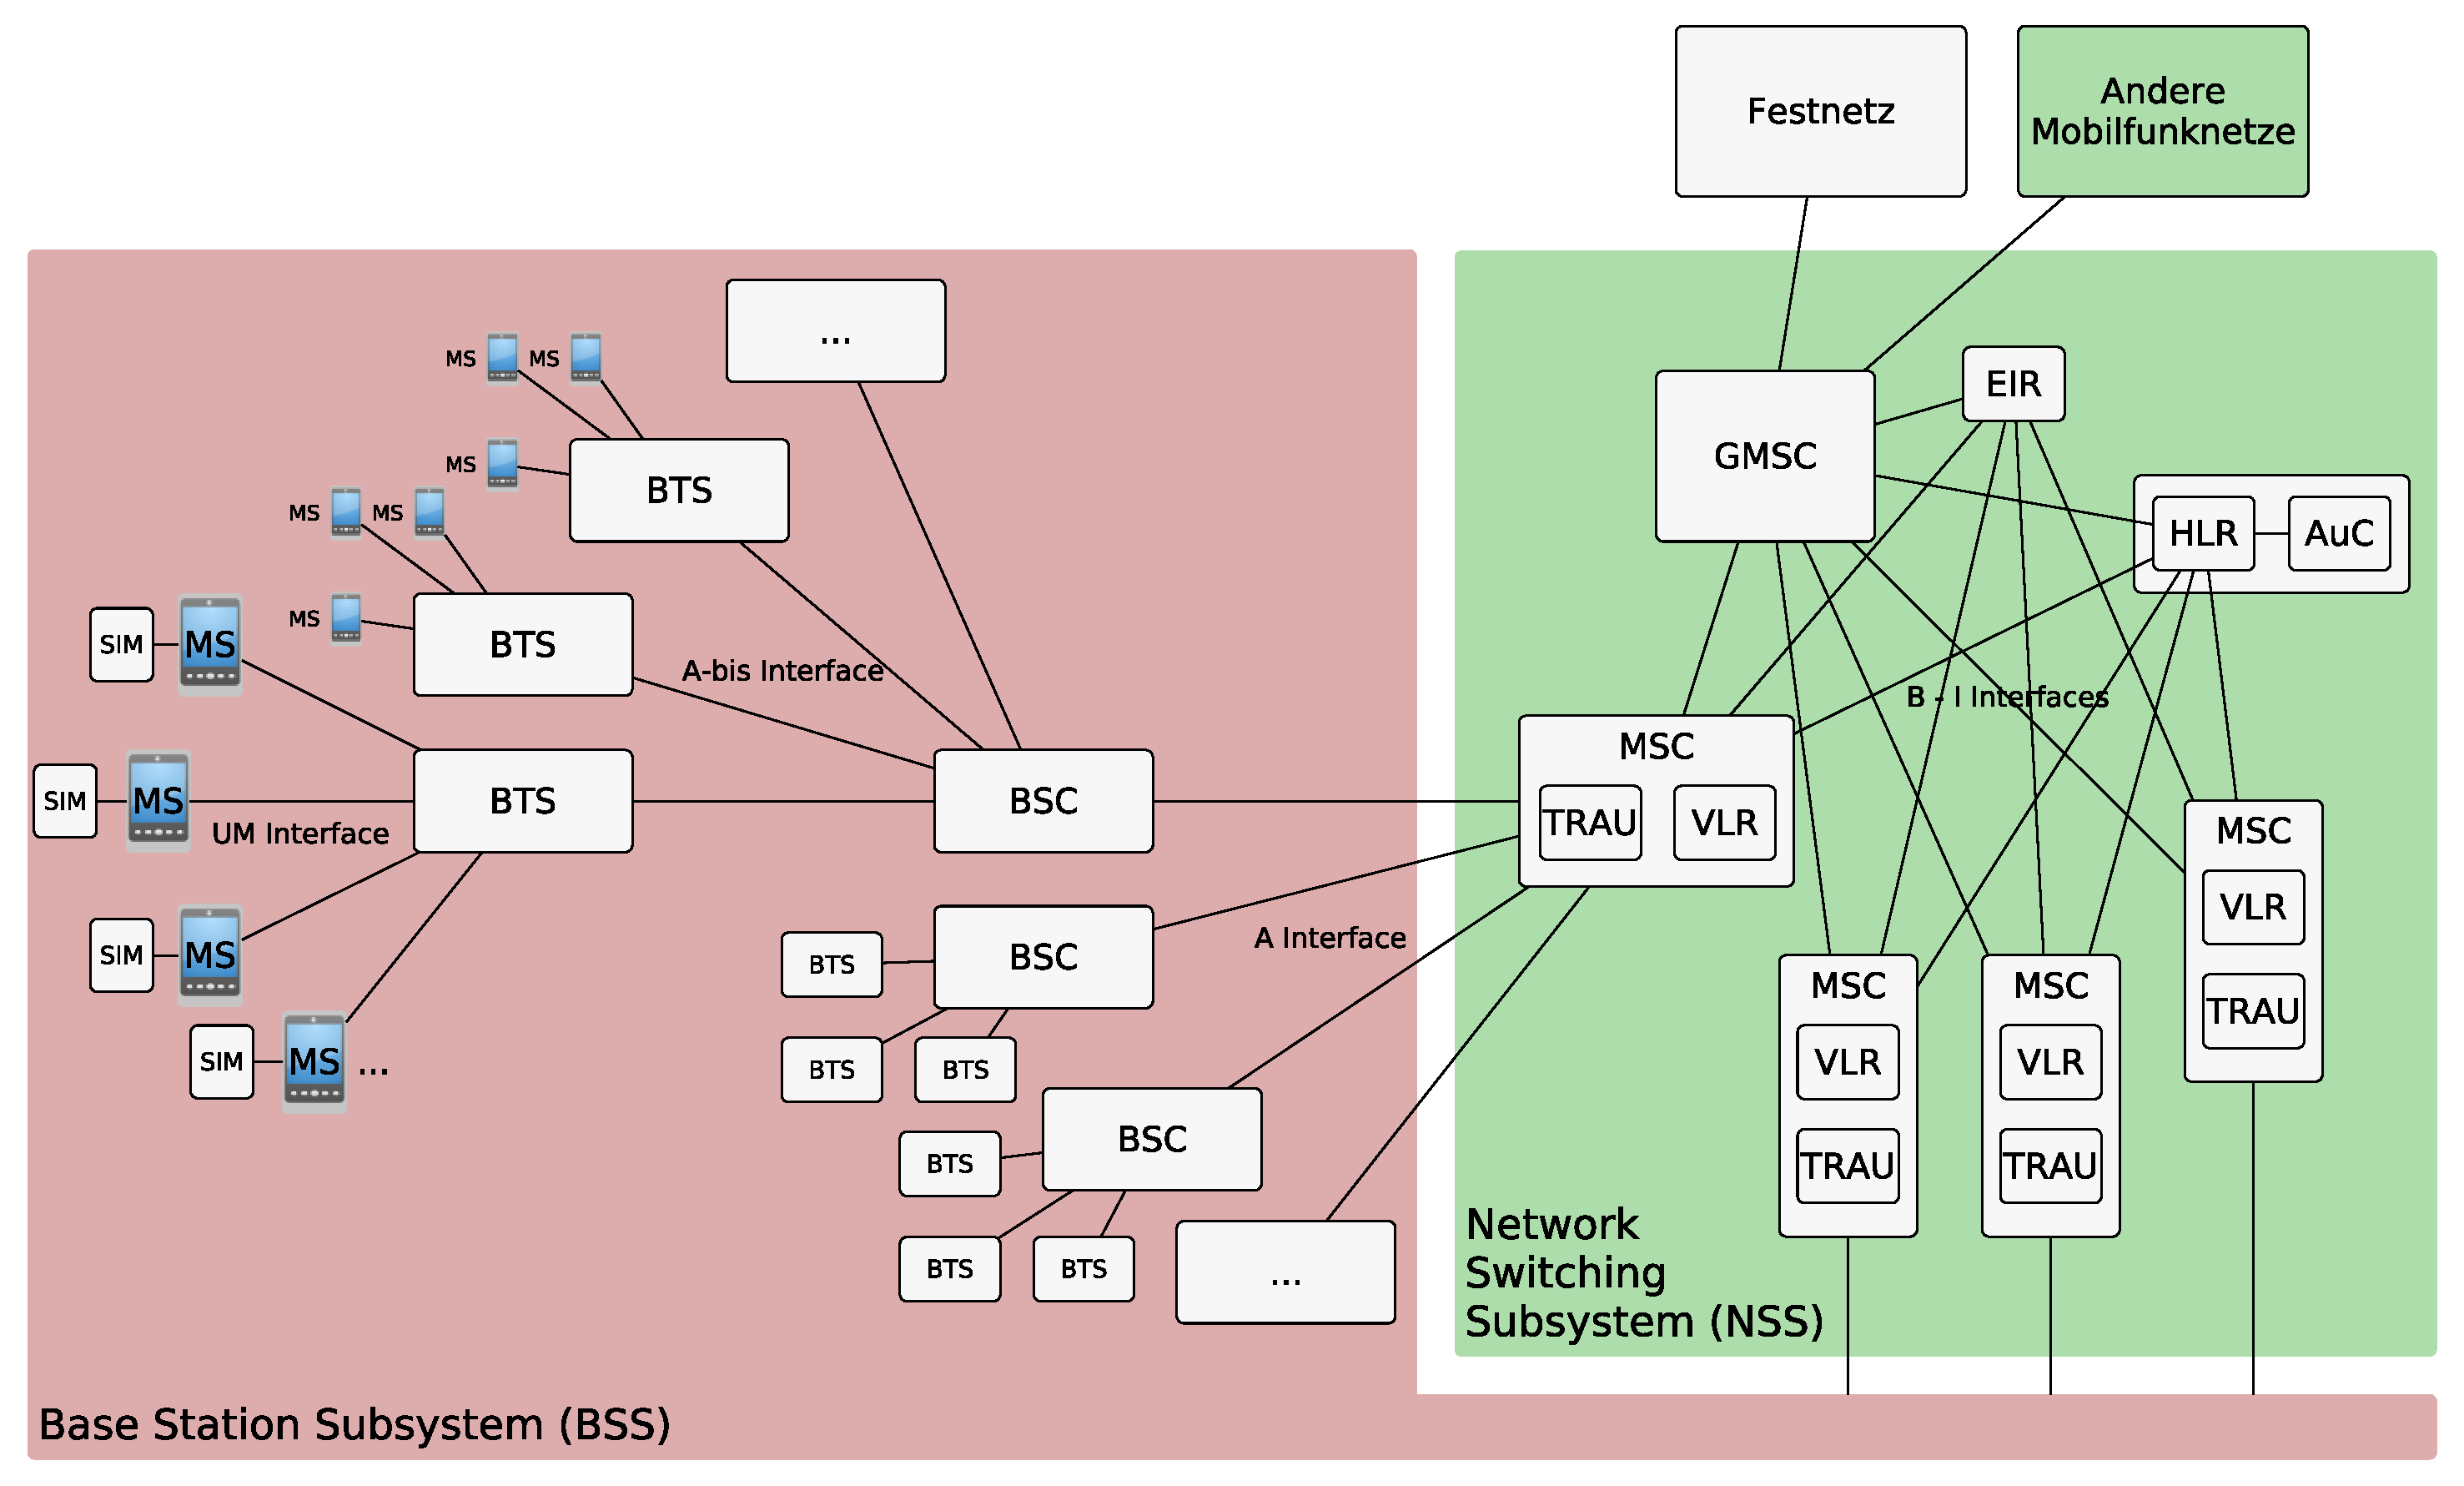
\includegraphics[width=1.0\linewidth]{figures/gsm_network_architecture.pdf}
\end{figure}

\begin{description}
\item[\acused{TRAU}\acs{TRAU} - \acl{TRAU}] Die \ac{TRAU} transkodiert \ac{GSM}-kodierte Sprachdaten in das im Netzwerk verwendete \ac{ISDN} Format (ITU-T A-law). Obwohl sie funktionell dem \ac{BSS} zugeordnet ist, kann sie entweder zwischen \ac{BTS} und \ac{BSC}, oder zwischen \ac{BSC} und \ac{MSC} eingebaut werden. Meist wird sie direkt im \ac{MSC} integriert, da dann weniger \ac{TRAU} Einheiten benötigt werden und Bandbreite auf dem Abis und A Interface gespart wird. \ac{GSM} kodierte Sprachdaten brauchen 13kBit/s, \ac{ISDN} kodierte 64kBit/s. \citep[Kap. 5.2.1]{eberspacher:2008:gsm-architecture}
\item[\acused{EIR}\acs{EIR} - \acl{EIR}] Das \ac{EIR} ist eine optionale Datenbank, die für die Verwaltung von Teilnehmer- und Gerätenummern zuständig ist. Hier werden die \acp{IMEI} von Geräten, die als gestohlen gemeldet wurden, auf einer Blacklist geführt. Diesen kann dann ein Zugriff zum Netz verwehrt werden.
\item[\acused{GMSC}\acs{GMSC} - \acl{GMSC}] Das \ac{GMSC} verbindet mehrere \acp{MSC} mit anderen Mobilfunknetzen und dem Festnetz. Es ist zuständig für die Vermittlung von Anrufen und Nachrichten zwischen diesen. Für Routing zwischen den \acp{PLMN} hat es innerhalb des \ac{SS7} Zugriff auf das \ac{HLR} und \ac{EIR}. In der Regel wird ein reguläres \ac{MSC} zusätzlich an andere \acp{PLMN} angebunden und um die Gateway Funktionalität erweitert.
\item[Abis Schnittstelle]
Die Abis Schnittstelle verbindet \ac{BTS} und \ac{BSC} über E-1 Leitungen. Neben der Weiterleitung von Anwenderdaten erlaubt sie über entsprechende Protokolle die Konfiguration des Transceivers sowie Allokation von Frequenzen im \ac{BTS}.
\item[A Schnittstelle] Das A Interface dient dem Datenaustausch zwischen \ac{BTS} und \ac{MSC}. Letzteres kann darüber Konfigurationsnachrichten an das \ac{BSS} schicken und Nutzerdaten weiterleiten.
\item[B-I Schnittstellen]
Hierbei handelt es sich um Interfaces, die zur Kommunikation zwischen Komponenten des \ac{NSS} definiert wurden. Die Komponenten sind über ein \ac{SS7}-Netzwerk miteinander verbunden und kommunizieren über verschiedene \ac{MAP} Protokolle.
\end{description}

\section{GSM Protokolle und Schnittstellen} \label{hdl:a_schnittstellen_protokolle}

\begin{figure}[H]
  \begin{center}
    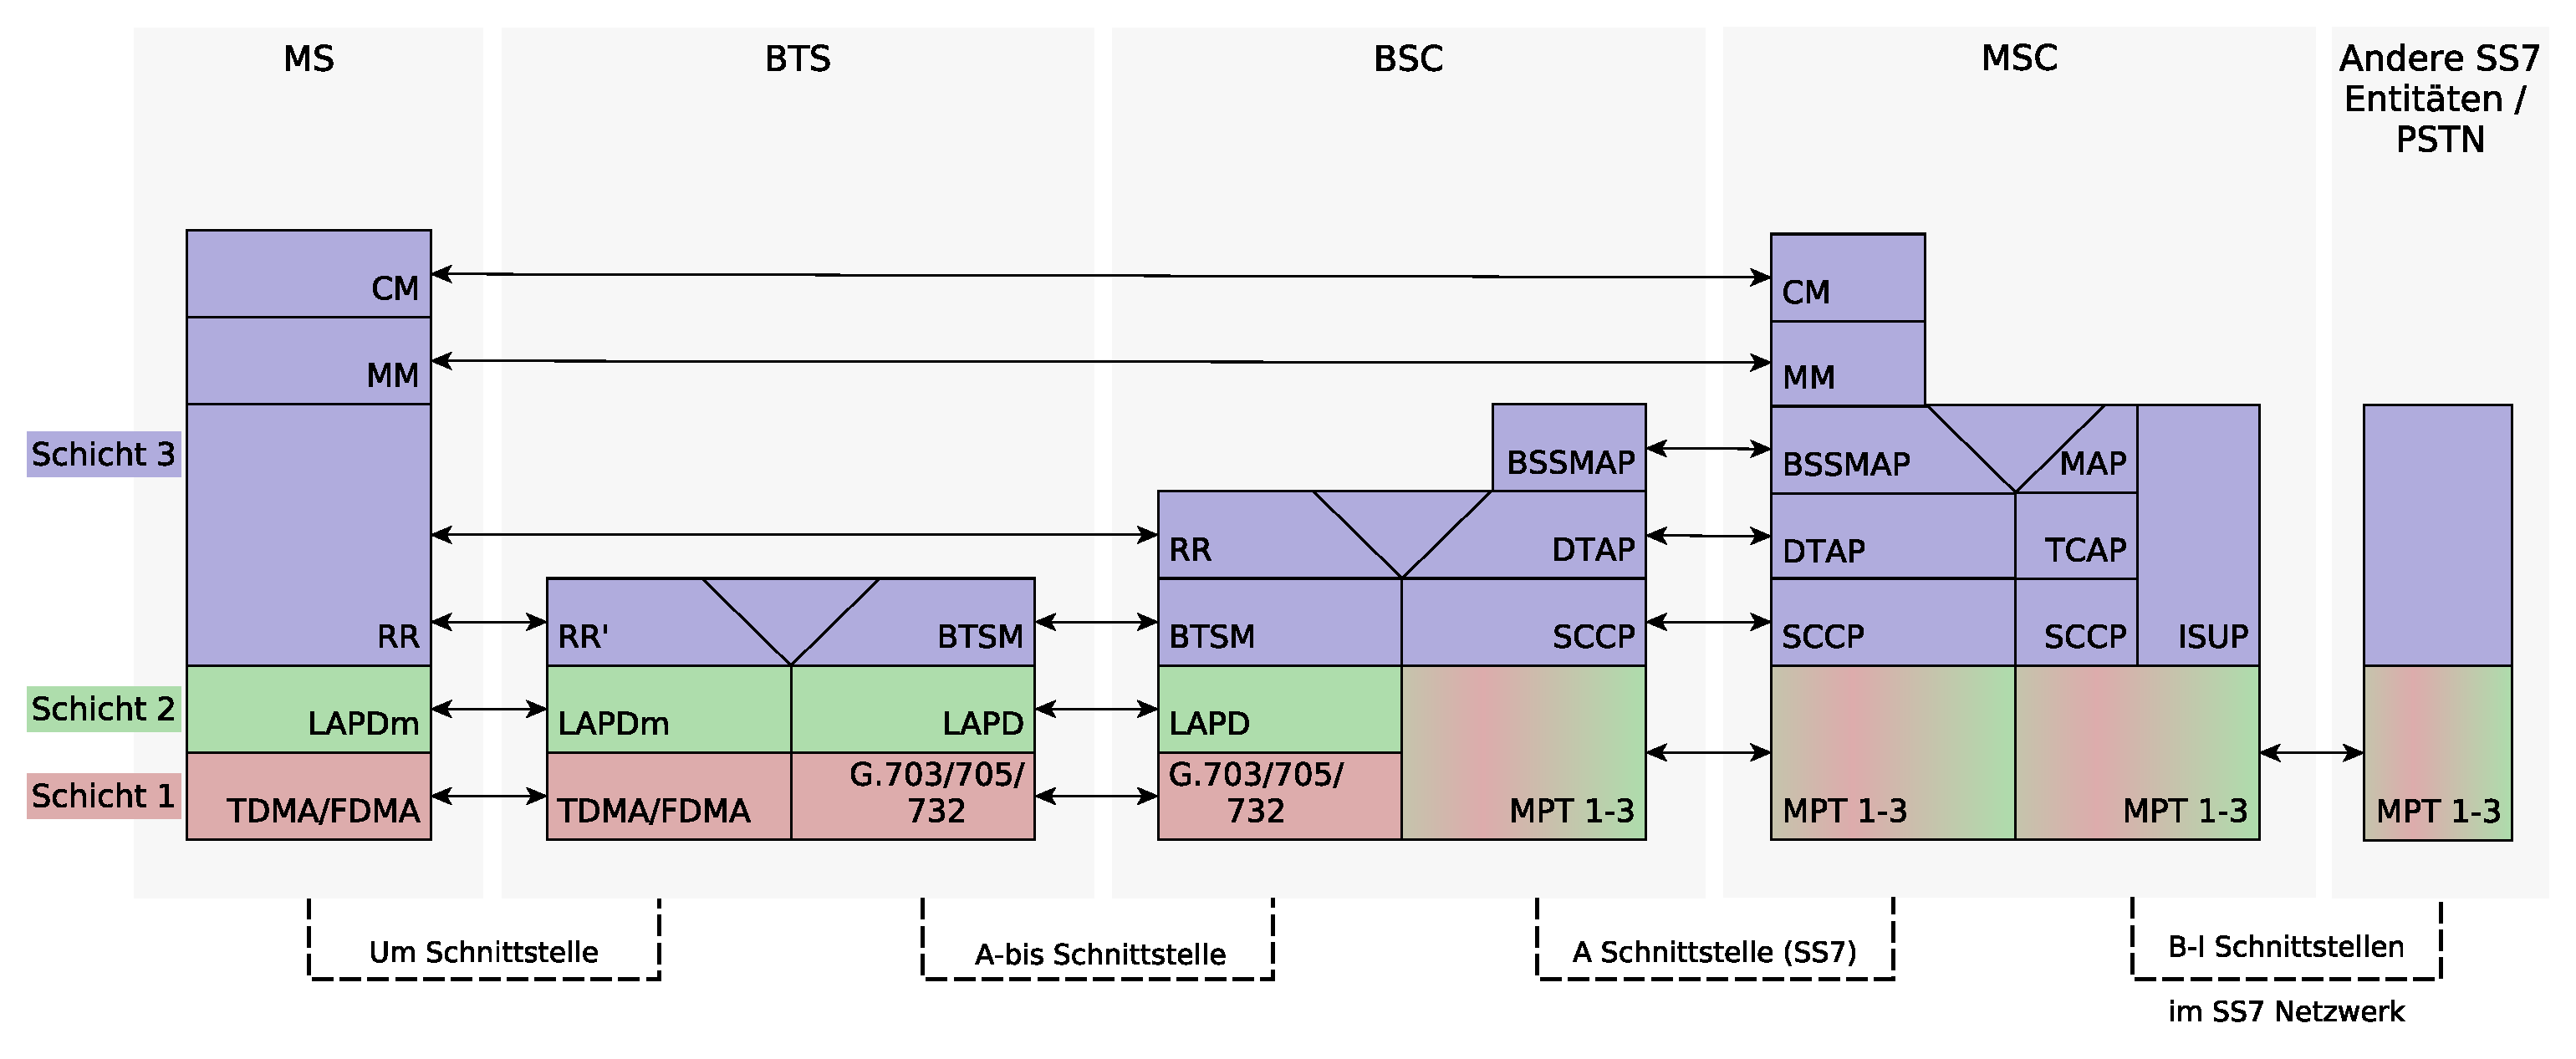
\includegraphics[width=1.0\textwidth]{figures/gsm_protocol_stack.pdf}
  \end{center}
\end{figure}

\subsection{TDMA/FDMA} \label{hdl:a_tdma_fdma}

\ac{GSM} verwendet als Phasenmodulation \ac{GMSK}, um das Spektrum bei Modulation eines digitalen Signals effektiv auszunutzen \citepauthor{3gpp:05.04}. Dadurch kann das in \ac{GSM}-900 zur Verfügung stehende Frequenzband, von 890.0-915.0 MHz für Uplink und 935.0-960.0 MHz für Downlink, in jeweils 124 Trägerfrequenzen mit 200kHz Abstand eingeteilt werden. Über die \acp{ARFCN} werden einer \ac{BTS} Funkkanäle für Uplink und Downlink zugeordnet. \citep{schnabel2003kommunikationstechnik}

In \citetauthor[Kap. 4.3]{3gpp:05.02} wird das in \ac{GSM} verwendete \ac{TDMA} Verfahren spezifiziert. Ein \ac{TDMA} Frame (4.615 ms) besteht darin aus 8 Zeitschlitzen mit einer Zeitdauer von 577 $\mu$s, sogenannten physikalischen Kanälen. Ein mit jedem \ac{TDMA} Frame inkrementierter Zähler gibt an, in welchem Frame man sich gerade befindet.

\begin{figure}[H]
  \begin{center}
    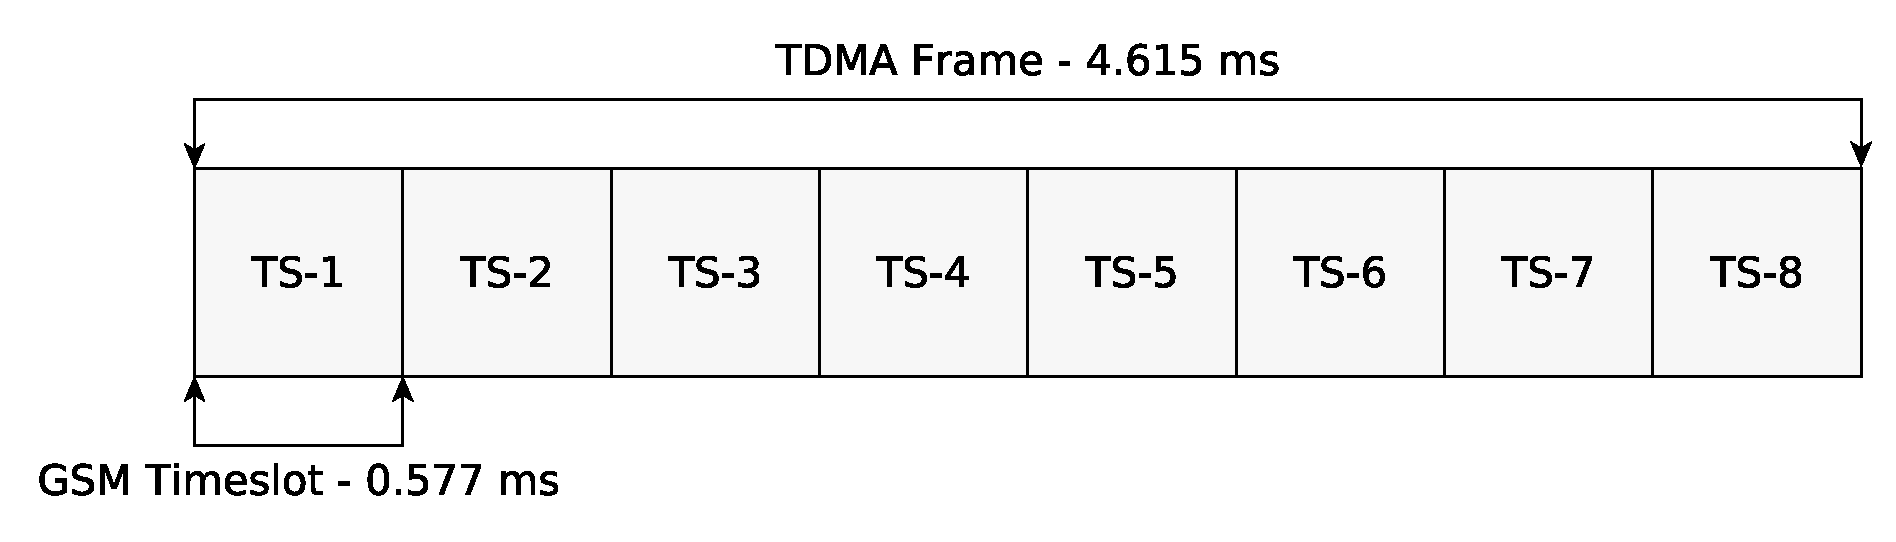
\includegraphics[width=1.0\textwidth]{figures/gsm_timeslots.pdf}
  \end{center}
  \caption[TDMA-Zeitschlitze in GSM]{\ac{TDMA}-Zeitschlitze in \ac{GSM}, nach \citepauthor[Kap. 4.3]{3gpp:05.02}} \label{fig:gsm-timeslots} 
\end{figure}

In einem Timeslot kann die Datenmenge von genau einem \ac{GSM}-Burst übertragen werden. Je nach Inhalt gibt es verschiedene Typen von Bursts, die in \citetauthor[5.2]{3gpp:05.02} nachgelesen werden können. Der Aufbau eines \acp{NB} ist in \autoref{fig:normal_burst} dargestellt. Neben kodierten Daten enthalten Bursts auch eine "`Guard Period"' am Ende, die keine Information mehr enthält, als Puffer zwischen den Timeslots.

Der Uplink wird um 3 Zeitschlitze verzögert mit dem Downlink synchronisiert, damit die \acp{MS} genug Zeit haben auf empfangene Daten zu reagieren. Physikalische Kanäle können unterschiedliche Aufgaben wie Broadcasting (\ac{BCCH}), Signalisierung (\ac{CCCH}) und Sprachdatenübertragung (\ac{TCH}) zugewiesen werden. Durch die Konfiguration von bis zu 7 Sprachkanälen pro Trägerfrequenz können je Trägerfrequenz mehrere Sprachverbindungen gleichzeitig übertragen werden. \citep{schnabel2003kommunikationstechnik}

In der Regel wird TS-0 eine Kombination aus \ac{BCCH} und \ac{CCCH}, TS-1 \ac{CCCH} zugeordnet und die restlichen Kanäle für Sprach- oder Datenübertragung verwendet.

\subsection{Abis Interface} \label{hdl:a_abis}

Die \ac{BSS}-interne Schnittstelle zwischen \ac{BTS} und \ac{BSC} ist nicht standardisiert. Das Abis Interface ermöglicht die Steuerung und Konfiguration der \ac{BTS} über \ac{BTSM} und die Weiterleitung transparenter \ac{RR}, \ac{MM} und \ac{CM} Nachrichten.

Die physikalische Schicht besteht meist aus einer kabelgebundenen Verbindung nach \citetauthor{itu:g.703} (oder 705 / 732) mit 2,048 MBit/s (Europa) oder 1,544 MB/s (USA). Die Bandbreite wird über \ac{TDMA} in 30 Zeitschlitze für Sprache und Daten und zwei Zeitschlitze für Synchronisation und Signalisierung unterteilt.

Für die Datensicherungsschicht wird das \ac{ISDN} Protokoll \ac{LAPD} verwendet. Dessen Aufgabe ist der zuverlässige Datentransfer zwischen \ac{BTS} und \ac{BSC} auf dem D-Kanal. Der D-Kanal ist in \ac{ISDN} der Kanal zur Übertragung von Steuerinformationen. Für \ac{ISDN} ist das Protokoll in \citetauthor{itu:q.920} und \citetauthor{itu:q.921} spezifiziert, die \ac{GSM} Adaption findet man in \citetauthor{3gpp:08.56}.

\ac{LAPD} umfasst folgende allgemeine Funktionen:
\begin{itemize}
\item Bereitstellung von einem oder mehreren \ac{LAPD}-Verbindungen auf dem D-Kanal
\item Bereitstellung einer zuverlässigen Verbindung auf dem D-Kanal
\item Ablaufkontrolle
\item Flußkontrolle
\item Fehlererkennung und Korrekturmechanismen
\item Benachrichtigung von Layer 3 Einheiten bei fatalen Fehlern
\end{itemize}

Für Layer 3 werden mehrere \ac{LAPD}-Verbindungen zur Verfügung gestellt, die über verschiedene \acp{SAPI} unterschieden werden. Jede \ac{SAPI} verwendet dabei ein eigenes Protokoll. Layer 3 auf der A-bis Schnittstelle ist in \citetauthor{3gpp:08.58} beschrieben.

Übersicht über die Protokolle der \acp{SAPI}:
\begin{description}
\item [SAPI 0, \acf{RSL}] wird für Weiterleitung des Datenverkehrs von und an die Luftschnittstelle verwendet, also \ac{RR}-Signalisierungsnachrichten und die transparenten \ac{CC} und \ac{CM} Nachrichten.
\item [SAPI 62, \acf{OML}] wird für Verwaltung, Konfiguration und Überwachung des \ac{BTS} und seiner Transceivereinheiten verwendet.
\item [SAPI 63, \acf{L2ML}] ist für die dynamische Verwaltung von \acp{TEI} und der Adressierung der Transceivern zuständig.
\end{description}

\subsection{A Interface} \label{hdl:a_a_interface}

Das A Interface liegt zwischen \ac{BSC} und \ac{MSC}. Der Protokollstack basiert auf dem \ac{SS7} Standard, der auch für die Signalisierung im restlichen \ac{NSS} verwendet wird. Die physikalische Verbindung ist, wie beim Abis Interface, kabelgebunden mit 2,048 oder 1,544 MBit/s. Sie wird über \ac{TDMA} in 32 Kanäle unterteilt. Davon werden 30 für Datenübertragung und zwei für Signalisierung verwendet. Bei Positionierung der \ac{TRAU} im \ac{BSC} \ac{TRAU} benötigt ein Sprachkanal im \ac{ISDN} Format 64 kBit/s und füllt damit einen kompletten Slot aus. Es können also bis zu 30 Verbindungen gleichzeitig unterstützt werden. Sitzt die \ac{TRAU} hingegen im \ac{MSC}, braucht ein Sprachkanal nur 16 kBit/s. Dadurch sind mehr gleichzeitige Verbindungen möglich. 

Schicht 1 und 2 verwenden in \ac{SS7} definierte \ac{MTP}, die eine zuverlässige Verbindung zwischen \ac{BSC} und \ac{MSC} gewährleisten.

\ac{SCCP} ermöglicht auf Schicht 3 eine globale Adressierung von Elementen im \ac{SS7}-Netzwerk. Mit \ac{BSSMAP} Nachrichten kann das \ac{BSS} vom \ac{MSC} konfiguriert und überwacht werden. Des Weiteren stellt \ac{SCCP} verbindungslose und verbindungsorientierte Nachrichtenflüsse für \acf{RR}, \ac{CM} und \ac{MM} zur Verfügung.

\section{A5 Verschlüsselungsverfahren}\label{hdl:a_a5}
Von \ac{3GPP} aktuell (Stand 2017) spezifizierte, synchrone Verschlüsselungsverfahren auf der Funkschnittstelle.

\subsection{A5/0}
Wird A5/0 ausgehandelt, ist die Verbindung auf der Luftschnittstelle unverschlüsselt. In \citetauthor[4.8]{3gpp:03.20} wird zwar ausdrücklich erwähnt, dass Mobiltelefonen die nur A5/0 unterstützen, abgewiesen werden sollen, umgekehrt gilt das aber nicht. So akzeptieren die meisten Handys eine unverschlüsselte Verbindung, wenn die \ac{BTS} diese fordert. Dem Benutzer wird das oft nicht signalisiert. 

A5/0 wird von echten \ac{BTS} der Netzbetreiber nicht verwendet, Angreifer mit falschen \ac{BTS} können diese Schwachstelle aber nutzen.

\subsection{A5/1}

A5/1 ist eine 1987 für \ac{GSM} entwickelte Stromchiffre und war bis zur Veröffentlichung von A5/3 der sicherste verfügbare Algorithmus.

Die geringe Schlüsselänge von 64 Bit in Kombination mit Schwachstellen gegen Angriffe mit bekanntem Klartext macht den Algorithmus verwundbar \citep{golic1997cryptanalysis}. \citet{nohl2010wideband} führte auf der 27C3 vor, dass eine A5/1 verschlüsselte Verbindung mit handelsüblicher und kostengünstiger Hardware in Echtzeit gebrochen werden kann. Da die für den Angriff verwendeten Rainbow Tables veröffentlicht wurden, kann der Angriff seitdem mit geringem eigenen Aufwand von beliebigen Angreifern ausgeführt werden.

A5/1 wird trotz seiner Schwächen auch 2017 noch mit einem Anteil von ca. 50\% im \ac{GSM}-Netz verwendet \citep{gsmmap:secrep-ger}. 

\subsection{A5/2}

A5/2 ist eine Stromchiffre, die 1989 für Exportländer von \ac{GSM} entwickelt wurde. Mit nur 50 Bit Entropie im kryptografischen Schlüssel ist der Algorithmus deutlich schwächer als A5/1 und wurde von \citet{barkan2003instant} in Echtzeit geknackt.

Um 2007 wurde in den \ac{3GPP} Meetings festgelegt, dass A5/2 offiziell nicht mehr von neuen Mobiltelefonen und im \ac{GSM}-Netz unterstützt werden soll. Alle Netzbetreiber davon zu überzeugen sollte aber noch bis 2008 dauern. \citep{osmocom:withdrawal-a52}

\subsection{A5/3, GEA3}

Der A5/3 Algorithmus basiert auf der Blockchiffre KASUMI \citepauthor{3gpp:35.202} und wurde 2002 in \citetauthor{3gpp:55.216} im Zuge der \ac{EDGE}/\ac{EGPRS} Entwicklung als Nachfolger von A5/1 spezifiziert. In \ac{UMTS} wird der Algorithmus standardmäßig unterstützt, in \ac{GSM} musste er von den Netzbetreibern erst nachgerüstet werden, was den Einzug in \ac{GSM}-Netzwerken hinauszögerte. In Deutschland wurde A5/3 erst 2013 von der Deutschen Telekom zusätzlich zu A5/1 für \ac{GSM} eingeführt \citep{telekom:a53-gsm}.

\autoref{fig:fig-a53-encryption} veranschaulicht das Mapping der Input- und Outputparameter auf die KASUMI-KGCORE-Funktion. Dabei ist \ac{Kc} der vom \ac{A8} aus dem geheimen Schlüssel des Mobilfunkteilnehmers generierte Schlüssel und COUNT die Framenumber der zu verschlüsselnden Nachricht. Die Framenumber kann den maximalen Wert von 2715648 erreichen, wofür die 22 verwendeten Bits ausreichen. A5/3 verwendet KASUMI nur mit 64 Bit Entropie, der von KASUMI verlangte Schlüsselparameter mit 128 Bit wird durch Konkatenation von zwei 64 Bit Schlüsseln erreicht.

Als Ergebnis liefert die Funktion zwei Blöcke BLOCK1 und BLOCK2 mit 114 Bits, die für die Verschlüsselung und Entschlüsselung von je einem Uplink und Downlink Burst verwendet werden. Verschlüsselt wird über binäre Addition der Datenbits mit dem Schlüsselstrom.

\begin{figure}[H]
  \begin{center}
    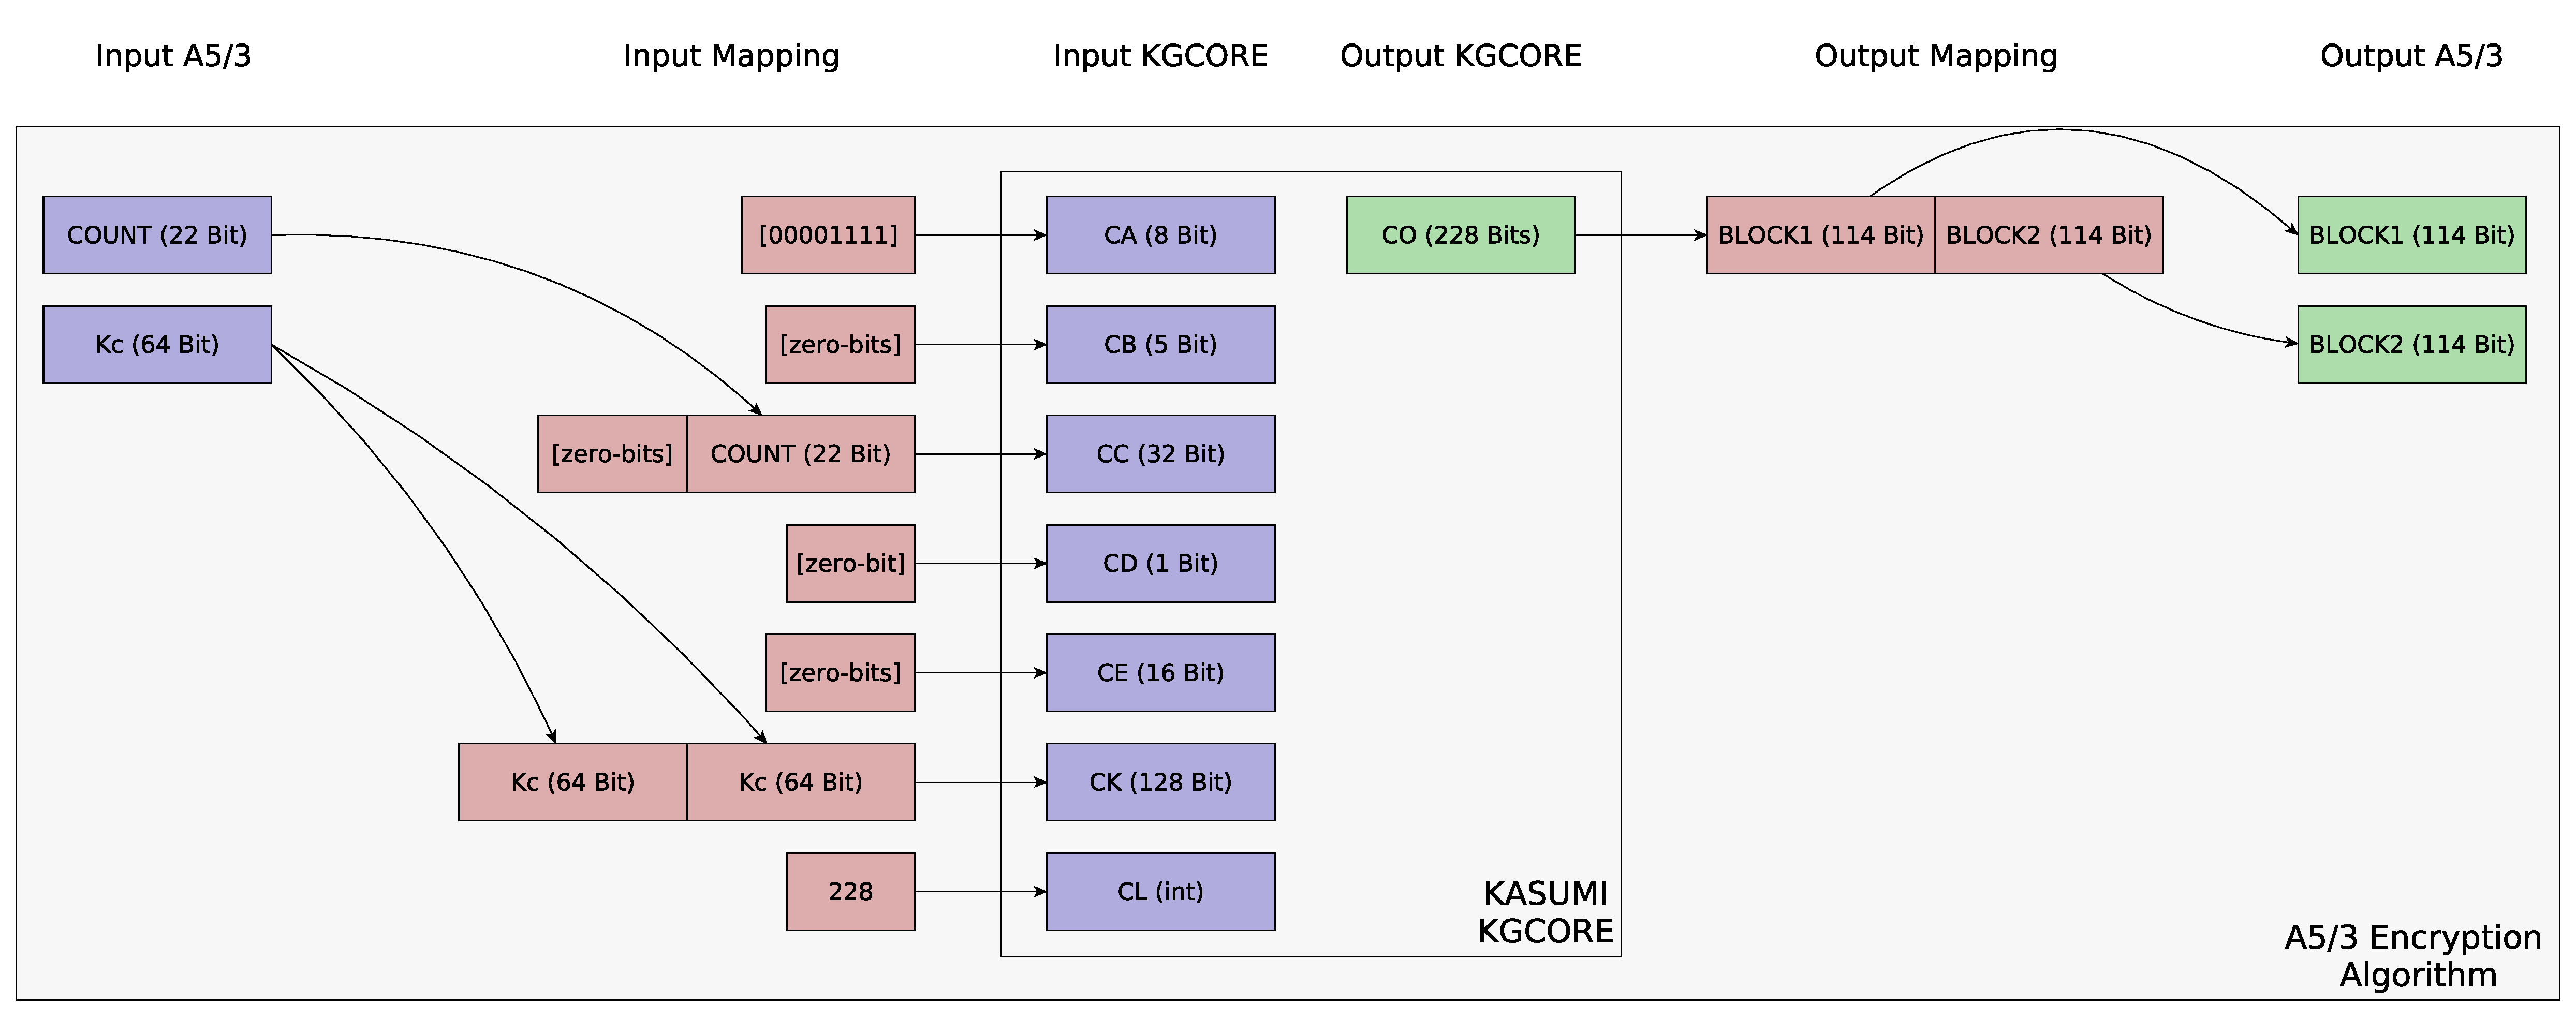
\includegraphics[width=1.0\textwidth]{figures/a53_encryption.pdf}
  \end{center}
  \caption[Das Parameter Mapping von A5/3 auf die Kasumi-KGCORE-Funktion]{Das Parameter Mapping von A5/3 auf die Kasumi-KGCORE-Funktion, erstellt mit yEd} \label{fig:fig-a53-encryption}
\end{figure}

Kasumi konnte von \citet{dunkelman2010practical} geknackt werden. Allerdings kann der Angriff nicht auf seine Verwendung im A5/3 Algorithmus angewendet werden. Trotz seiner geringen effektiven Schlüssellänge von 64 Bit gilt er deshalb als relativ sicher. Die Schlüssellänge macht ihn jedoch grundsätzlich verwundbar für Bruteforce Attacken. \citep{nohl2014mobile}

A5/3 ist der sicherste aktuell in \ac{GSM}-Netzwerken verwendete Algorithmus und deshalb für den vorgestellten Angriff von besonderem Interesse.

\subsection{A5/4, GEA4}
Ein in \citetauthor{3gpp:55.226} spezifiziertes Verschlüsselungsverfahren, das wie A5/3 auf KASUMI basiert, im Gegensatz zu diesem aber die kompletten verfügbaren 128 Bit als Schlüssel verwendet.

Der Algorithmus wird in aktuellen 2G Netzwerken nicht verwendet.

\subsection{GIA5, GEA5}
Ein recht neuer Algorithmus, der 2016 in \citetauthor{3gpp:55.226} spezifiziert wurde.

Der Algorithmus wird in aktuellen 2G Netzwerken nicht verwendet.

\section{Frequency-Hopping}

Frequency-Hopping kann in \ac{GSM} optional verwendet werden, um für die Übertragung von Daten ein breiteres Frequenzspektrum zu benutzen. Dabei springt die Trägerfrequenz innerhalb eines bestimmten Bereichs. Die Sprungparameter werden in einer bestehenden Verbindung vom \ac{BTS} vorgegeben und dem Endgerät im \ac{SDCCH} mitgeteilt.

Damit werden auf der Luftschnittstelle häufige frequenzbedingte Übertragungsprobleme verringert und das Signal-Rausch-Verhältnis verbessert. Frequency Hopping ist - solange eine nicht vorhersehbare Hopping Sequenz verwendet wird - auch eine sicherheitsrelevante Funktion. Die Zuweisung von abgefangenen Signalen zu einer Verbindung wird ohne das Wissen der verwendeten Sprungsequenz erschwert.

\ac{GSM} definiert in \citetauthor{3gpp:05.02} folgende Parameter für Frequency Hopping:
\begin{description}
\item[\acf{MA}] Eine Liste von erlaubten Sprungfrequenzen für das Mobiltelefon. Es können maximal 63 Frequenzen angegeben werden.
\item[\acf{HSN}] Legt die in der Zelle verwendete Sprungsequenz fest. Es können 64 verschiedene \acp{HSN} verwendet werden. \ac{HSN} = 0 bedeutet zyklisches Springen, die Werte 1 bis 63 geben verschiedene pseudo-zufällige Sequenzen vor.
\item[\acf{MAIO}] Legt die Startfrequenz fest, auf der die \ac{MS} zu Senden beginnt. Der Wert kann zwischen 0 und der maximal in \ac{MA} festgelegten Anzahl an unterstützten Frequenzen liegen.
\end{description}
\chapter{Umsetzung -- Anhang}
In diesem Kapitel werden verschiedene Anhänge mit Bezug zur theoretischen oder praktischen Umsetzung aufgelistet.

\section{Einrichtung des Testnetzwerks mit virtueller Um-Schnittstelle}\label{hdl:a_einrichtung_testumgebung}

In diesem Abschnitt wird die Einrichtung und Konfiguration des Testnetzwerks, in dem der \ac{MitM}-Angriff durchgeführt wurde, erklärt.

Die Testumgebung wurde in der Masterarbeit auf Linux-Debian Jessie eingerichtet. Folgende Osmocom-Bibliotheken müssen entweder über Github, Autoconf und Automake selbst kompiliert und installiert oder über verfügbare Nigthly-Builds des Paketmanagers installiert werden.
\begin{itemize}
\item libosmocore -- \url{git://git.osmocom.org/libosmocore.git}, Branch: master
\item libosmo-abis -- \url{git://git.osmocom.org/libosmo-abis.git}, Branch: master
\item libosmo-netif -- \url{git://git.osmocom.org/libosmo-netif.git}, Branch: master
\end{itemize}
Folgende Projekte müssen über Github, Autoconf und Automake selbst kompiliert werden:
\begin{itemize}
\item osmoBSC -- \url{git://git.osmocom.org/openbsc.git}, Branch: master
\item osmoBTS -- \url{git://git.osmocom.org/osmo-bts}, Branch: stumpf/virt-phy
\item osmocomBB -- \url{git://git.osmocom.org/osmocom-bb}, Branch: stumpf/virt-phy
\item osmoMITM -- \url{https://github.com/BastusIII/osmo-mitm}, Branch: master
\end{itemize}
Beim Kompilieren und der Installation obiger Komponenten und ihrer Abhängigkeiten kann man sich an folgenden Anleitungen im Osmocom Wiki orientieren:
\begin{itemize}
\item \url{osmocom.org/projects/cellular-infrastructure/wiki/SDR_OsmoTRX_network_from_scratch}
\item \url{osmocom.org/projects/openbsc/wiki/Building_OpenBSC}
\item \url{osmocom.org/projects/cellular-infrastructure/wiki/Build_from_source}
\end{itemize}

Sind die Bibliotheken installiert und konnten die Projekte erfolgreich kompiliert werden, geht es an die Konfiguration. 

Aus dem osmoBSC Projekt wird die osmoNITB Anwendung benötigt. Für die Verwendung von osmoNITB mit dem virtuellen \ac{Um} ist keine spezielle Konfiguration notwendig, es kann also die Standardkonfiguration benutzt werden. Es empfiehlt sich aber folgende Parameter anzupassen:\\

\begin{lstlisting}[boxpos=c, frame=single, language=bytetxt, numbers=none, basicstyle=\tiny\ttfamily, tabsize=1 ]
network
 auth policy accept-all !!accept all subscribers!!
 authorized-regexp .* !!wildcard needs to be set to really accept all subscribers!!
 encryption a5 0 !!don't use encryption, as its currently not supported by virtual Um!!
 (...)
 bts 0
  type sysmobts !!declaring the type as sysmobts will work with the virtual bts!!
  (...)
  trx 0 
   (...)
   timeslot 0 
    phys_chan_config CCCH+SDCCH4 
    hopping enabled 0 !!hopping should be disabled for all timeslots, not only for this one!!
    (...)
nitb
 subscriber-create-on-demand !!create subscribers in hlr automatically!!
 subscriber-create-on-demand random 1 24
 assign-tmsi !!activates tmsi assignment and reallocation!!
\end{lstlisting}

Aus osmoBTS wird die Anwendung für die virtuelle \ac{BTS} benötigt. Eine Beispielkonfigurationsdatei ist im Projektordner unter \texttt{src/osmo-bts-virtual/example\_configs} zu finden. Für die Kommunikation mit dem \ac{BSC} über die Abis-Schnittstelle muss die \texttt{ipa unit-id} mit dem gleichen Wert wie in osmoNITB konfiguriert sein. Informationen dazu finden sich auch in den oben referenzierten Wiki-Links. Für das virtuelle \ac{Um} müssen folgende Einträge konfiguriert werden, der Rest ist Standard.\\

\begin{lstlisting}[boxpos=c, frame=single, language=bytetxt, numbers=none, basicstyle=\tiny\ttfamily, tabsize=1 ]
(...)
phy 0
 virtual-um ms-multicast-group 224.0.0.1 !!the multicast ip address, the bts will send to!!
 virtual-um ms-udp-port 4729 !!4729 will be recognized by Wireshark as GSMTAP!!
 virtual-um bts-multicast-group 225.0.0.1 !!the multicast ip address, the bts will receive from!!
 virtual-um bts-udp-port 4729
(...)
\end{lstlisting}

Aus osmocomBB wird die Anwendung für die physikalische Schicht des \ac{Um} \texttt{virtphy} und die L23-App \texttt{mobile} benötigt. \texttt{virtphy} wird über Kommandozeilenparameter erst beim Aufruf des Programms konfiguriert. Für \texttt{mobile} findet sich eine Beispielkonfigurationsdatei im Projektordner in \texttt{src/host/virt\_phy/example\_configs}. Wichtig ist die Aktivierung der \texttt{test-sim} Option, da die Implementierung der virtuellen physikalischen Schicht den Zugriff auf die \ac{SIM}-\ac{APDU} nicht über das \ac{L1CTL}-Socket anbietet.\\

\begin{lstlisting}[boxpos=c, frame=single, language=bytetxt, numbers=none, basicstyle=\tiny\ttfamily, tabsize=1 ]
ms 1
 layer2-socket /tmp/osmocom_l2 !!the path to the L1CTL socket used!!
 sim test !!define that the test-sim should be used!!
(...)
test-sim
 imsi 901700000000403 !!can be chosen as wished!!
 ki comp128 12 34 56 78 90 1b cd ef 12 34 56 78 90 ab cd ef !!can be chosen as wished!!
 no barred-access
 rplmn 262 42 0x0001 !!can be used to set the preferred network to avoid the long network search at startup!!
 hplmn-search everywhere
exit
(...)
\end{lstlisting}

Der \ac{MitM} im virtuellen \ac{Um} aus osmoMITM wird ebenfalls über Kommandozeilenparameter gestartet.

Nach der Konfiguration müssen die Anwendungen in folgender Reihenfolge und mit folgenden Kommandozeilenparametern gestartet werden. Es wird angenommen die Projekte befinden sich alle im Ordner \texttt{\textasciitilde/Osmocom} im Home-Verzeichnis des Benutzers und die angepassten Konfigurationsdateien sowie die SQLite-Datenbank für das \ac{HLR} von osmoNITB in \texttt{\textasciitilde/Osmocom/config}.\\

\begin{lstlisting}[boxpos=c, frame=single, language=bytetxt, numbers=none, basicstyle=\footnotesize\ttfamily, tabsize=1 ]
NITB: 
~/Osmocom/openbsc/src/osmo-nitb/osmo-nitb 
  -c ~/Osmocom/config-files/openbsc-virtual.cfg
  -l ~/Osmocom/config-files/hlr.sqlite3 
  -P -C
      
BTS: 
~/Osmocom/osmo-bts/src/osmo-bts-virtual/osmo-bts-virtual 
  -c ~/Osmocom/config-files/osmobts-virtual.cfg    
      
MS layer1: 
~/Osmocom/osmocom-bb/src/host/virt\_phy/src/virtphy 
  --l1ctl-sock /tmp/osmocom\_l2 
  --port 4729 
  --ul-tx-grp 226.0.0.1 
  --dl-rx-grp 226.0.0.2

MS L23-App mobile: 
~/Osmocom/osmocom-bb/src/host/layer23/src/mobile/mobile 
  -c ~/Osmocom/config-files/osmocom-bb-mobile-virtual-ms1.cfg

MITM:
~/Osmocom/osmo-mitm/src/osmomitmsetupmanip 
  --ul-rx-grp 226.0.0.1 
  --dl-tx-grp 226.0.0.2 
  --ul-tx-grp 225.0.0.1 
  --dl-rx-grp 224.0.0.1 
  --dump-msgs 
  --imsi-victim 901700000000403 
  --msisdn-called 017518181818 
  --msisdn-attacker 017517171717 
  --msisdn-to-setup-offset 11
\end{lstlisting}

Wenn alle Anwendungen korrekt gestartet wurden, kann über Wireshark der Nachrichtenverkehr auf dem virtuellen \ac{Um} aufgezeichnet werden. Es bietet sich an, die Nachrichten dazu nach \texttt{gsmtap} oder \texttt{lapdm} zu filtern.

Die Konfigurationen von \texttt{nitb}, \texttt{bts} und \texttt{mobile} können nach dem Start über deren \ac{VTY}-Schnittstelle eingesehen und angepasst werden. Das \ac{VTY} von \texttt{mobile} wird des Weiteren verwendet, um den Anruf vom Opfer aus zu starten. Ist der \ac{MitM} wie oben konfiguriert, dann leitet er ausgehende Anrufe der \ac{IMSI} \texttt{901700000000403} an die \ac{MSISDN} \texttt{017518181818} zur \ac{MSISDN} \texttt{017517171717} um. Der Anruf vom Opfer, bzw. \texttt{mobile} sollte also an die Telefonnummer \texttt{017518181818} erfolgen. Auf das \ac{VTY} von \texttt{mobile} kann, sofern dessen Port nicht verändert wurde, mit telnet zugegriffen werden (\texttt{telnet localhost 4247}). Mit dem \ac{VTY}-Befehl \texttt{call 1 017518181818} kann der Anruf gestartet werden.

\section{L1CTL-Routinen in osmocomBB}\label{hdl:a_l1ctl-routines}

\begin{table}[H]
\begin{adjustbox}{max width={0.8\textwidth}, padding=4pt 2pt 4pt 0pt, center}
\begin{tabular}{|p{5cm}|p{5cm}|p{5cm}|}
\hline
\rowcolor[HTML]{F7F7F7}
\textbf{L1CTL Routine}                  & \textbf{Beschreibung}                                                                     & \textbf{Status}                                                                                             \\ \hline
\texttt{L1CTL\_FBSB\_REQ/CONF}                   & Cumulated request to sync frequency to a given ARFCN and then start time synchronization. & Implemented                                                                                                 \\ \hline
\texttt{L1CTL\_DATA\_IND/REQ/CONF}               & Transmit / receive data on one of the signaling channels FACCH, SDCCH, SACCH.             & Implemented                                                                                                 \\ \hline
\texttt{L1CTL\_RACH\_REQ/CONF}                   & Transmit data on RACH.                                                                    & Implemented                                                                                                 \\ \hline
\texttt{L1CTL\_TRAFFIC\_REQ/CONF/IND}            & Transmit traffic on a TCH/F or TCH/R.                                                     & Implemented                                                                                                 \\ \hline
\texttt{L1CTL\_PM\_REQ/CONF}                     & Start power measurement on given frequencies.                                             & Implemented                                                                                                 \\ \hline
\texttt{L1CTL\_NEIGH\_PM\_REQ/IND}               & Start neighbor power measurement.                                                         & Not implemented Currently not used as handover is not yet implemented                                       \\ \hline
\texttt{L1CTL\_TCH\_MODE\_REQ/CONF}              & Configure TCH mode and audio mode.                                                        & Status: Implemented but unused, as we do not support speech recording and transmission yet.                 \\ \hline
\texttt{L1CTL\_CCCH\_MODE\_REQ/CONF}             & Configure CCCH combined / non-combined mode.                                              & Implemented                                                                                                 \\ \hline
\texttt{L1CTL\_RESET\_IND/REQ/CONF}              & Request or indicate a layer 1 full reset or scheduler reset.                              & Implemented, used to tell L23 that physical layer has started up e.g.                                       \\ \hline
\texttt{L1CTL\_ECHO\_REQ/CONF}                   & Print something out on the display.                                                       & Not implemented, but also not needed for the virtual physical layer.                                        \\ \hline
\texttt{L1CTL\_SIM\_REQ/CONF}                    & Forward a command to the SIM card.                                                        & Not implemented SIM cards are currently not supported. We use the mobile's test-sim option to simulate one. \\ \hline
\texttt{L1CTL\_DM\_EST\_REQ/L1CTL\_DM\_REL\_REQ} & Handle state chance from idle to dedicated mode and vice-versa.                           & Implemented                                                                                                 \\ \hline
\texttt{L1CTL\_DM\_FREQ\_REQ}                    & Handle frequency change for a dedicated channel.                                          & Not implemented, as frequency hopping is not yet supported.                                                 \\ \hline
\texttt{L1CTL\_PARAM\_REQ}                       & Change timing advance value and / or sending power.                                       & Not implemented, but also not needed for the virtual physical layer.                                        \\ \hline
\texttt{L1CTL\_CRYPTO\_REQ}                      & Configure the key and algorithm used for cryptographic operations.                        & Not implemented, as encryption is not yet supported.                                                        \\ \hline
\end{tabular}
\end{adjustbox}\caption[L1CTL-Routinen und deren Implementierungsstand in osmocomBB]{\ac{L1CTL}-Routinen und deren Implementierungsstand in osmocomBB}\label{hdl:a_l1ctl_routines}
\end{table}

\section{Manipulation von Beispieldaten mit \texttt{dummycoder} und \texttt{xor\_hexstrings.py}}\label{hdl:a_example_setup_manip}

Die Ausgabe wurde von Hand formatiert und farblich gekennzeichnet und wird nicht so von der Testroutine generiert. Die Datenmanipulation und ihre Auswirkung auf die Kodierungsschritte ist rot gekennzeichnet, Kommentare sind blau dargestellt. Die Testroutine kann mit beliebigen Daten ausgeführt werden und liegt im osmoMITM Projekt im Ordner \texttt{tests/setup\_manip\_test}. Das Skript \texttt{setup\_manip\_exec.sh} ruft die Programme \texttt{dummycoder} und \texttt{xor\_hexstrings.py} mehrmals auf, um die Ausgabe zu generieren. Dort müssen die Dateien \texttt{data}, \texttt{data\_manip}, \texttt{cipherstream} und \texttt{remainder} liegen und mit Daten in Form von Hexstrings befüllt sein. Alle Ergebnisse werden im Ordner \texttt{tests/setup\_manip\_test/test\_data} auch als Textdateien abgespeichert.\\

\begin{lstlisting}[caption={Die Kommandozeilenausgabe von \texttt{setup\_manip\_test} aus osmoMITM}, boxpos=c, frame=single, language=bytetxt, numbers=none, basicstyle=\tiny\ttfamily, tabsize=1 ]
!!Hinweise:!!
!!data:             Originalnachricht als Plaintext!!
!!data_manip:       Manipulierte Nachricht als Plaintext!!
!!remainder:        Rest des Firecodes in GSM!!
!!cipherstream:     Schlüsselstrom !!
!!.crc:             Daten nach Anwendung von Firecode!!
!!.cc:              Daten nach Anwendung von Convolutional Coding!!
!!XORcipherstream:  Stromverschlüsselung!!

01 20 51 03 45 04 04 60  02 00 81 5e 07 81 10 57
81 81 81 81 15 01 01                             !!= data!!

01 20 51 03 45 04 04 60  02 00 81 5e 07 81 10 57 
@1@1 81 81 81 15 01 01                             !!= data_manip!!

00 00 00 00 00 00 00 00  00 00 00 00 00 00 00 00 
@9@0 00 00 00 00 00 00                             !!= dataXORdata_manip!!

00 00 00 00 00 00 00 00  00 00 00 00 00 00 00 00 
@9@0 00 00 00 00 00 00 2f  93 7e 5f 2f 00          !!= dataXORdata_manip.crc!!

00 00 00 00 00 00 00 00  00 00 00 00 00 00 00 00 
00 00 00 00 00 00 00 ff  ff ff ff ff 00          !!= remainder!!

00 00 00 00 00 00 00 00  00 00 00 00 00 00 00 00 
@9@0 00 00 00 00 00 00 d0  6c 81 a0 d0 00          !!= dataXORdata_manip.crcXORremainder!!

01 20 51 03 45 04 04 60  02 00 81 5e 07 81 10 57 
81 81 81 81 15 01 01 f8  b8 1c ef e5 00          !!= data.crc!!

01 20 51 03 45 04 04 60  02 00 81 5e 07 81 10 57 
@1@1 81 81 81 15 01 01 28  d4 9d 4f 35 00          !!= dataXORdata_manip.crcXORremainderXORdata.crc!!

01 20 51 03 45 04 04 60  02 00 81 5e 07 81 10 57 
@1@1 81 81 81 15 01 01 28  d4 9d 4f 35 00          !!= data_manip.crc!!

00 00 00 00 00 00 00 00  00 00 00 00 00 00 00 00 
00 00 00 00 00 00 00 00  00 00 00 00 00          !!= dataXORdata_manip.crcXORremainderXORdata.crcXORdata_manip.crc!!

!!TEST1 - CHECK == 0 OK!!

00 03 42 3c 37 bc 4f 0e  47 c7 bf 34 f0 34 c9 cc 
00 0d 3c 00 d3 c3 78 55  0c 3a 50 c3 4c 4f 37 85 
@80 4c@ 9c c3 9c c3 9c c3  4c 78 bf 03 4f 03 @42 ef@ 
@24 4b 20 6b 4b 19 4d 44@  bf                      !!= [dataXORdata_manip.crcXORremainderXORdata.crc].cc!!

00 03 42 3c 37 bc 4f 0e  47 c7 bf 34 f0 34 c9 cc 
00 0d 3c 00 d3 c3 78 55  0c 3a 50 c3 4c 4f 37 85 
50 c3 9c c3 9c c3 9c c3  4c 78 bf 03 4f 03 a6 90
1d 60 c3 a8 da e5 a9 3b  bf                       !!= data.cc!!

00 00 00 00 00 00 00 00  00 00 00 00 00 00 00 00 
00 00 00 00 00 00 00 00  00 00 00 00 00 00 00 00 
00 00 00 00 00 00 00 00  00 00 00 00 00 00 00 00 
00 00 00 00 00 00 00 00  00                       !!= [dataXORdata_manip.crcXORremainderXORdata.crc].ccXORdata_manip.cc!!

!!TEST2 - CHECK == 0 OK!!

00 00 00 00 00 00 00 00  00 00 00 00 00 00 00 00 
00 00 00 00 00 00 00 00  00 00 00 00 00 00 00 00 
@d0 8f@ 00 00 00 00 00 00  00 00 00 00 00 00 @0d d5@ 
@93 81 49 69 3b 56 4e d5@  43                       !!= [dataXORdata_manip].cc!!

00 00 00 00 00 00 00 00  00 00 00 00 00 00 00 00 
00 00 00 00 00 00 00 00  00 00 00 00 00 00 00 00 
00 00 00 00 00 00 00 00  00 00 00 00 00 00 e9 aa 
aa aa aa aa aa aa aa aa  43                       !!= remainder.cc!!

00 00 00 00 00 00 00 00  00 00 00 00 00 00 00 00 
00 00 00 00 00 00 00 00  00 00 00 00 00 00 00 00 
@d0 8f@ 00 00 00 00 00 00  00 00 00 00 00 00 @e4 7f@ 
@39 2b e3 c3 91 fc e4 7f@  00                       !!= [dataXORdata_manip].ccXORremainder.cc!!

00 03 42 3c 37 bc 4f 0e  47 c7 bf 34 f0 34 c9 cc 
00 0d 3c 00 d3 c3 78 55  0c 3a 50 c3 4c 4f 37 85 
@80 4c@ 9c c3 9c c3 9c c3  4c 78 bf 03 4f 03 @42 ef@ 
@24 4b 20 6b 4b 19 4d 44@  bf                       !!= [dataXORdata_manip].ccXORremainder.ccXORdata.cc!!

00 03 42 3c 37 bc 4f 0e  47 c7 bf 34 f0 34 c9 cc 
00 0d 3c 00 d3 c3 78 55  0c 3a 50 c3 4c 4f 37 85 
@80 4c@ 9c c3 9c c3 9c c3  4c 78 bf 03 4f 03 @42 ef@ 
@24 4b 20 6b 4b 19 4d 44@  bf                       !!= data_manip.cc!!

00 00 00 00 00 00 00 00  00 00 00 00 00 00 00 00 
00 00 00 00 00 00 00 00  00 00 00 00 00 00 00 00 
00 00 00 00 00 00 00 00  00 00 00 00 00 00 00 00 
00 00 00 00 00 00 00 00  00                       !!= [dataXORdata_manip].ccXORremainder.ccXORdata.ccXORdata_manip.cc!!

!!TEST3 - CHECK == 0 OK!!

12 34 56 78 90 ab cd ef  12 34 56 78 90 ab cd ef 
12 34 56 78 90 ab cd ef  12 34 56 78 90 ab cd ef 
12 34 56 78 90 ab cd ef  12 34 56 78 90 ab cd ef 
12 34 56 78 90 ab cd ef  11                       !!= cipherstream!!

12 37 14 44 a7 17 82 e1  55 f3 e9 4c 60 9f 04 23 
12 39 6a 78 43 68 b5 ba  1e 0e 06 bb dc e4 fa 6a 
42 f7 ca bb 0c 68 51 2c  5e 4c e9 7b df a8 6b 7f 
0f 54 95 d0 4a 4e 64 d4  ae                       !!= data.ccXORcipherstream!!

12 37 14 44 a7 17 82 e1  55 f3 e9 4c 60 9f 04 23 
12 39 6a 78 43 68 b5 ba  1e 0e 06 bb dc e4 fa 6a 
@92 78@ ca bb 0c 68 51 2c  5e 4c e9 7b df a8 @8f 00@ 
@36 7f 76 13 db b2 80 ab@  ae                       !!= data_manip.ccXORcipherstream!!

00 00 00 00 00 00 00 00  00 00 00 00 00 00 00 00 
00 00 00 00 00 00 00 00  00 00 00 00 00 00 00 00 
@d0 8f@ 00 00 00 00 00 00  00 00 00 00 00 00 @e4 7f@ 
@39 2b e3 c3 91 fc e4 7f@  00                       !!= [dataXORdata_manip].ccXORremainder.cc!!

12 37 14 44 a7 17 82 e1  55 f3 e9 4c 60 9f 04 23 
12 39 6a 78 43 68 b5 ba  1e 0e 06 bb dc e4 fa 6a 
@92 78@ ca bb 0c 68 51 2c  5e 4c e9 7b df a8 @8f 00@ 
@36 7f 76 13 db b2 80 ab@  ae                       !!= [dataXORdata_manip].ccXORremainder.ccXORdata.ccXORcipherstream!!

00 00 00 00 00 00 00 00  00 00 00 00 00 00 00 00 
00 00 00 00 00 00 00 00  00 00 00 00 00 00 00 00 
00 00 00 00 00 00 00 00  00 00 00 00 00 00 00 00 
00 00 00 00 00 00 00 00  00                       !!= [dataXORdata_manip].ccXORremainder.ccXORdata.ccXORcipherstreamXOR!!
                                                    !!data_manip.ccXORcipherstream!!

!!TEST4 - CHECK == 0 OK!!
\end{lstlisting}
\chapter{Relevante GSM-Abläufe} \label{hdl:grundlagen_ablufe}

Im Folgenden werden verschiedene Abläufe in \ac{GSM} anhand von Nachrichtenflussdiagrammen oder Wireshark-Mitschnitten aufgelistet.

\section{\acl{RR} Connection Establishment} \label{hdl:grundlagen_rr-conn-est}

Neben den \ac{BCCH} und \ac{CCCH} gibt es in \ac{GSM} noch die dedizierten logischen Kanäle, bei denen eine Verbindung zwischen je einem \ac{MS} und einem \ac{BTS} aufgebaut wird. Der interne Nachrichtenaustausch zwischen den Protokollschichten läuft über \acp{SAP}.

Um bidirektional über einen solchen Kanal kommunizieren zu können, ist der Aufbau einer \ac{LAPDm} und darauf aufbauend einer \ac{RR} Verbindung notwendig. Die Signalisierung, die zur Einrichtung und Auflösung einer \ac{RR}-Verbindung nötig ist, wird in \autoref{fig:rr-conn-est} dargestellt.

\begin{figure}[H]
  \begin{center}
    \includegraphics[width=1.00\textwidth]{figures/gsm_rr-chan-est-rel.pdf}
  \end{center}
  \caption[Nachrichtenfluss von RR-Verbindungsaufbaus und Release]{Nachrichtenfluss von \ac{RR}-Verbindungsaufbau und Release} \label{fig:rr-conn-est}
\end{figure}

\begin{description}
\item[1] Der Verbindungsaufbau wird durch ein \texttt{RR-ESTABLISH-REQ} Primitive vom $\ac{MM}_{MS}$ an das \ac{SAP} des $\ac{RR}_{MS}$ in Auftrag gegeben. Entweder initiativ vom \ac{MS}, oder als Reaktion einer eingehenden Paging Nachricht auf dem \ac{PCH}.
\item[2] $\ac{RR}_{MS}$ lässt daraufhin von der physikalischen Schicht auf dem \ac{RACH} eine \texttt{CHANNEL-REQUEST}-Nachricht an $\ac{RR}_{Netzwerk}$ schicken. Wir sehen in \autoref{fig:interface-physical-layer}, dass diese einen \ac{SAP} direkt für \ac{RR} zur Verfügung stellt, die Datensicherungsschicht \ac{LAPDm} wird dabei übergangen.
\item[3] $\ac{RR}_{Netzwerk}$ reserviert entsprechende Ressourcen auf einem der dedizierten Kanäle. Das ist bei Early und Late-Assignment ein \ac{SDCCH} und bei Very-Early-Assignment bereits der \ac{TCH}. Über den \ac{AGCH} werden $\ac{RR}_{MS}$ in einer \texttt{IMMEDIATE-ASSIGNMENT}-Nachricht anschließend Informationen zum reservierten Kanal mitgeteilt. Schicht 2 wird wieder übergangen.
\item[4] Nach Erhalt des Immediate-Assignments wechselt das \ac{MS} in den "`Dedicated Mode"' und empfängt nur noch Nachrichten auf dem zugewiesenen dedizierten Kanal. \ac{BCCH}, \ac{CCCH} werden ignoriert. Eine zuverlässige Verbindung (\autoref{hdl:einfuehrung-gsm_schnittstellen_protokolle-um_interface-layer2}) wird von $L2_{MS}$ über die \ac{LAPDm}-Nachricht \ac{SABM} im unacknowledged Mode initiiert \citepauthor[3.8.2]{3gpp:04.06}.
\item[5] \ac{SABM} trägt dabei den kompletten von $\ac{MM}_{MS}$ in Auftrag gegebenen Service Request (\texttt{L3-SERVICE-REQUEST}) mit sich, was "`piggybacking"' genannt wird. Nachdem $L2_{Netzwerk}$ über den \ac{SAP} mit einer \texttt{DL-ESTABLISHED-IND} $\ac{RR}_{Netzwerk}$ über die Einrichtung der zuverlässigen Verbindung informiert hat, schickt dieses den Service Request weiter an $\ac{MM}_{Netzwerk}$. 
\item[6] Mit der \ac{LAPDm}-Nachricht \ac{UA} wird $L2_{MS}$ angewiesen, nun in den Acknowledged Information Transfer Mode zu wechseln. Ab dann werden durchnummerierte \ac{I}-Frames geschickt und die Verbindung ist durch die Retransmission Prozeduren, \ac{ACK} und \ac{REJ}-Nachrichten von Schicht 2 vor Paketverlust geschützt.
\item[7] Durch entsprechende \ac{SAP} Confirm Primitives werden $\ac{RR}_{MS}$ und $\ac{MM}_{MS}$ über die aufgebaute zuverlässige Verbindung informiert. Schicht 3 kann nun über \ac{LAPDm} auf diese zugreifen und Daten übertragen. Im Anschluss kann die Signalisierung für Authentifizierung und Verschlüsselung ablaufen, wofür die zuverlässige Verbindung benötigt wird. \citepauthor[3.3]{3gpp:04.18} \citepauthor[Figure A.1 ff.]{3gpp:24.007}
\item[8] In der Abbildung initiiert $\ac{MM}_{Netzwerk}$ das Auflösen der Verbindung mit einem \texttt{RR-RELEASE-REQ}, was aber auch vom \ac{MS} ausgehen kann.
\item[9] Der \texttt{CHANNEL-RELEASE-REQUEST} wird an $\ac{RR}_{MS}$ weitergeleitet.
\item[10] $\ac{RR}_{MS}$ reagiert indem es $\ac{MM}_{MS}$ über die beendete Verbindung informiert und $L2_{MS}$ befiehlt, diese aufzulösen. $L2_{MS}$ kommt dem nach und informiert über \ac{LAPDm} \texttt{DISC} $L2_{Netzwerk}$ über den Wechsel in den Unacknowledged Information Transfer Mode, der mit einem \ac{UA} Frame bestätigt wird.
\item[11] Erhält $\ac{RR}_{MS}$ die Bestätigung über das Beenden der zuverlässigen Verbindung, wechselt das \ac{MS} vom "`Dedicated"' wieder in den "`Idle Mode"'. Es werden also wieder Nachrichten auf \ac{BCCH} und \ac{CCCH} empfangen und bearbeitet. \citepauthor[3.4.13]{3gpp:04.18} \citepauthor[Figure A.1 ff.]{3gpp:24.007}
\end{description} 

\section{Wireshark Mitschnitte}

Im Folgenden sind Mitschnitte des Nachrichtenverkehrs auf dem \ac{Um} aufgelistet. Mitschnitte \autoref{lst:real_bts_traffic_det_wireshark} und \autoref{lst:real_bts_traffic_short_wireshark} wurden von osmocomBB mit aktivem \ac{GSMTAP} Logging erstellt. Die Destination-\ac{IP}-Adresse ist deshalb immer das lokale Netzwerkinterface. \autoref{lst:mitm_attack_wireshark} zeigt den aufgezeichneten \ac{MitM}-Angriff auf dem virtuellen \ac{Um}. Dabei sind die \ac{MS} unter der \ac{IP}-Adresse 226.0.0.1 zu erreichen, der \ac{MitM} unter 226.0.0.1 und die \ac{BTS}. Da sowohl die Verbindung von \ac{MS} zu \ac{MitM}, als auch von \ac{MitM} zu \ac{BTS} aufgezeichnet wird, scheinen manche Nachrichten doppelt zu sein. In \autoref{lst:mitm_attack_wireshark} wurden die Details von interessanten Nachrichten aufgeklappt.

Der in Wireshark angewendete Filter für den detaillierten Nachrichtenverlauf mit \ac{LAPDm}"=Kontrollnachrichten ist: 
\begin{verbatim}
   !(gsmtap.chan_type == 137) 
&& !(gsmtap.chan_type == 136) 
&& !(gsm_a.dtap.msg_rr_type == 0x15) 
&& lapdm
\end{verbatim}
Für den detaillierten Nachrichtenverlauf mit \ac{LAPDm}-Kontrollnachrichten ist der Filter:
\begin{verbatim}
   !(lapdm.length_field == 0x01) 
&& !(gsmtap.chan_type == 137) 
&& !(gsmtap.chan_type == 136) 
&& !(gsm_a.dtap.msg_rr_type == 0x15) 
&& lapdm
\end{verbatim}

Kommentare in den Mitschnitten werden in blau angezeigt und sind nicht Teil der Nachrichten. Manipulierte Nachrichten in \autoref{lst:mitm_attack_wireshark} sind rot gekennzeichnet.\\

\begin{lstlisting}[caption={[Aufgezeichneter Nachrichtenverkehr mit E-plus BTS, kurz]Aufgezeichneter Nachrichtenverkehr mit E-plus \ac{BTS}, kurz (ohne \ac{LAPDm}-Kontrollnachrichten), generiert mit Filtern aus Wireshark-Mitschnitt}, label={lst:real_bts_traffic_short_wireshark}, boxpos=c, frame=single, language=bytetxt, numbers=none, basicstyle=\tiny\ttfamily, tabsize=1 ]
No.     Destination           Protocol 
    293 127.0.0.1             LAPDm    U P, func=SABM(DTAP) (MM) Location Updating Request 
    298 127.0.0.1             LAPDm    U F, func=UA(DTAP) (MM) Location Updating Request 
    299 127.0.0.1             LAPDm    I, N(R)=0, N(S)=0(DTAP) (MM) Identity Request 
    301 127.0.0.1             LAPDm    I, N(R)=1, N(S)=0(DTAP) (MM) Identity Response 
    303 127.0.0.1             LAPDm    I, N(R)=0, N(S)=1(DTAP) (MM) Identity Request 
    307 127.0.0.1             LAPDm    I, N(R)=2, N(S)=1(DTAP) (MM) Identity Response 
    309 127.0.0.1             LAPDm    I P, N(R)=1, N(S)=1(DTAP) (MM) Identity Request 
    313 127.0.0.1             LAPDm    I, N(R)=2, N(S)=2(DTAP) (MM) Authentication Request 
    323 127.0.0.1             LAPDm    I, N(R)=3, N(S)=2(DTAP) (MM) Authentication Response 
    329 127.0.0.1             LAPDm    I, N(R)=3, N(S)=3(DTAP) (RR) Ciphering Mode Command 
    331 127.0.0.1             LAPDm    I, N(R)=4, N(S)=3(DTAP) (RR) Ciphering Mode Complete 
    333 127.0.0.1             LAPDm    I, N(R)=4, N(S)=4(DTAP) (MM) Identity Request 
    335 127.0.0.1             LAPDm    I, N(R)=5, N(S)=4(DTAP) (MM) Identity Response 
    339 127.0.0.1             LAPDm    I, N(R)=5, N(S)=5(DTAP) (MM) Location Updating Accept 
    341 127.0.0.1             LAPDm    I, N(R)=6, N(S)=5(DTAP) (MM) TMSI Reallocation Complete 
    348 127.0.0.1             LAPDm    I, N(R)=5, N(S)=6 (Fragment)
    353 127.0.0.1             LAPDm    I P, N(R)=6, N(S)=6 (Fragment)
    355 127.0.0.1             LAPDm    I, N(R)=6, N(S)=7(DTAP) (MM) MM Information 
    357 127.0.0.1             LAPDm    I, N(R)=6, N(S)=0(DTAP) (RR) Channel Release 
   2987 127.0.0.1             LAPDm    U P, func=SABM(DTAP) (MM) CM Service Request 
   2992 127.0.0.1             LAPDm    U F, func=UA(DTAP) (MM) CM Service Request 
   2994 127.0.0.1             LAPDm    I, N(R)=0, N(S)=0(DTAP) (MM) Identity Request 
   2996 127.0.0.1             LAPDm    I, N(R)=1, N(S)=0(DTAP) (MM) Identity Response 
   2997 127.0.0.1             LAPDm    I, N(R)=0, N(S)=1(DTAP) (MM) Authentication Request 
   3007 127.0.0.1             LAPDm    I, N(R)=2, N(S)=1(DTAP) (MM) Authentication Response 
   3008 127.0.0.1             LAPDm    I P, N(R)=1, N(S)=1(DTAP) (MM) Authentication Request 
   3012 127.0.0.1             LAPDm    I, N(R)=2, N(S)=2(DTAP) (RR) Ciphering Mode Command 
   3014 127.0.0.1             LAPDm    I, N(R)=3, N(S)=2(DTAP) (RR) Ciphering Mode Complete 
   3023 127.0.0.1             LAPDm    I, N(R)=0, N(S)=0 (Fragment)
   3025 127.0.0.1             LAPDm    I, N(R)=0, N(S)=1 (Fragment)
   3029 127.0.0.1             GSM SMS  I, N(R)=0, N(S)=2(DTAP) (SMS) CP-DATA (RP) RP-DATA (MS to Network) 
   3030 127.0.0.1             LAPDm    I, N(R)=3, N(S)=0(DTAP) (SMS) CP-ACK 
   3033 127.0.0.1             GSM SMS  I, N(R)=3, N(S)=1(DTAP) (SMS) CP-DATA (RP) RP-ACK (Network to MS) 
   3037 127.0.0.1             LAPDm    I, N(R)=2, N(S)=3(DTAP) (SMS) CP-ACK 
   3040 127.0.0.1             LAPDm    I, N(R)=3, N(S)=3(DTAP) (RR) Channel Release 
   4630 127.0.0.1             LAPDm    U P, func=SABM(DTAP) (MM) CM Service Request 
   4635 127.0.0.1             LAPDm    U F, func=UA(DTAP) (MM) CM Service Request 
   4637 127.0.0.1             LAPDm    I, N(R)=0, N(S)=0(DTAP) (MM) Identity Request 
   4639 127.0.0.1             LAPDm    I, N(R)=1, N(S)=0(DTAP) (MM) Identity Response 
   4640 127.0.0.1             LAPDm    I, N(R)=0, N(S)=1(DTAP) (RR) Ciphering Mode Command 
   4645 127.0.0.1             LAPDm    I, N(R)=2, N(S)=1(DTAP) (RR) Ciphering Mode Complete 
   4646 127.0.0.1             LAPDm    I P, N(R)=1, N(S)=1(DTAP) (RR) Ciphering Mode Command 
   4650 127.0.0.1             LAPDm    I, N(R)=2, N(S)=2(DTAP) (CC) Setup 
   4654 127.0.0.1             LAPDm    I, N(R)=3, N(S)=2(DTAP) (CC) Call Proceeding 
   4658 127.0.0.1             LAPDm/GSM MAP I, N(R)=3, N(S)=3(DTAP) (CC) Facility (GSM MAP) invoke notifySS 
   4661 127.0.0.1             LAPDm    I, N(R)=3, N(S)=4 (Fragment)
   4663 127.0.0.1             LAPDm    I, N(R)=3, N(S)=5(DTAP) (RR) Assignment Command 
   4668 127.0.0.1             LAPDm    I, N(R)=0, N(S)=0(DTAP) (RR) Assignment Complete 
   4670 127.0.0.1             LAPDm    I, N(R)=1, N(S)=0(DTAP) (CC) Progress 
   4693 127.0.0.1             LAPDm    I, N(R)=1, N(S)=1(DTAP) (CC) Progress 
   4695 127.0.0.1             LAPDm    I, N(R)=1, N(S)=2(DTAP) (CC) Alerting 
   4732 127.0.0.1             LAPDm    I, N(R)=1, N(S)=3(DTAP) (CC) Connect 
   4736 127.0.0.1             LAPDm    I, N(R)=4, N(S)=1(DTAP) (CC) Connect Acknowledge 
   4777 127.0.0.1             LAPDm    I, N(R)=2, N(S)=4(DTAP) (CC) Disconnect 
   4781 127.0.0.1             LAPDm    I, N(R)=5, N(S)=2(DTAP) (CC) Release 
   4783 127.0.0.1             LAPDm    I, N(R)=3, N(S)=5(DTAP) (CC) Release Complete 
\end{lstlisting}

\begin{lstlisting}[caption={[Aufgezeichneter Nachrichtenverkehr mit E-plus BTS, lang]Aufgezeichneter Nachrichtenverkehr mit E-plus \ac{BTS}, detailliert (mit \ac{LAPDm}-Kontrollnachrichten), generiert mit Filtern aus Wireshark-Mitschnitt}, label={lst:real_bts_traffic_det_wireshark}, boxpos=c, frame=single, language=bytetxt, numbers=none, basicstyle=\tiny\ttfamily, tabsize=1 ]
No.     Destination           Protocol 
    293 127.0.0.1             LAPDm    U P, func=SABM(DTAP) (MM) Location Updating Request !!this RR-connection is for the LU!!
    298 127.0.0.1             LAPDm    U F, func=UA(DTAP) (MM) Location Updating Request 
    299 127.0.0.1             LAPDm    I, N(R)=0, N(S)=0(DTAP) (MM) Identity Request 
    300 127.0.0.1             LAPDm    S, func=RR, N(R)=1
    301 127.0.0.1             LAPDm    I, N(R)=1, N(S)=0(DTAP) (MM) Identity Response 
    303 127.0.0.1             LAPDm    I, N(R)=0, N(S)=1(DTAP) (MM) Identity Request 
    304 127.0.0.1             LAPDm    S, func=RR, N(R)=2
    306 127.0.0.1             LAPDm    S, func=RR, N(R)=1
    307 127.0.0.1             LAPDm    I, N(R)=2, N(S)=1(DTAP) (MM) Identity Response 
    309 127.0.0.1             LAPDm    I P, N(R)=1, N(S)=1(DTAP) (MM) Identity Request 
    310 127.0.0.1             LAPDm    S F, func=REJ, N(R)=2 !!identity response rejected by lapdm-> needs to be retransmitted!!
    311 127.0.0.1             LAPDm    S, func=RR, N(R)=2
    313 127.0.0.1             LAPDm    I, N(R)=2, N(S)=2(DTAP) (MM) Authentication Request 
    314 127.0.0.1             LAPDm    S, func=RR, N(R)=3
    323 127.0.0.1             LAPDm    I, N(R)=3, N(S)=2(DTAP) (MM) Authentication Response 
    329 127.0.0.1             LAPDm    I, N(R)=3, N(S)=3(DTAP) (RR) Ciphering Mode Command 
    330 127.0.0.1             LAPDm    S, func=RR, N(R)=4
    331 127.0.0.1             LAPDm    I, N(R)=4, N(S)=3(DTAP) (RR) Ciphering Mode Complete !!up from here everything in this
                                                                                            RR-connection is enciphered!!
    333 127.0.0.1             LAPDm    I, N(R)=4, N(S)=4(DTAP) (MM) Identity Request 
    334 127.0.0.1             LAPDm    S, func=RR, N(R)=5
    335 127.0.0.1             LAPDm    I, N(R)=5, N(S)=4(DTAP) (MM) Identity Response 
    339 127.0.0.1             LAPDm    I, N(R)=5, N(S)=5(DTAP) (MM) Location Updating Accept !!MS gets its TMSI here!!
    340 127.0.0.1             LAPDm    S, func=RR, N(R)=6
    341 127.0.0.1             LAPDm    I, N(R)=6, N(S)=5(DTAP) (MM) TMSI Reallocation Complete !!TMSI has been changed in MS!!
    348 127.0.0.1             LAPDm    I, N(R)=5, N(S)=6 (Fragment) !!some LAPDm frames are too big and will be fragmented!!
    349 127.0.0.1             LAPDm    S, func=RR, N(R)=7
    351 127.0.0.1             LAPDm    S, func=RR, N(R)=6
    353 127.0.0.1             LAPDm    I P, N(R)=6, N(S)=6 (Fragment)
    354 127.0.0.1             LAPDm    S F, func=REJ, N(R)=7
    355 127.0.0.1             LAPDm    I, N(R)=6, N(S)=7(DTAP) (MM) MM Information 
    356 127.0.0.1             LAPDm    S, func=RR, N(R)=0
    357 127.0.0.1             LAPDm    I, N(R)=6, N(S)=0(DTAP) (RR) Channel Release 
    358 127.0.0.1             LAPDm    S, func=RR, N(R)=1
    359 127.0.0.1             LAPDm    U P, func=DISC
    362 127.0.0.1             LAPDm    U F, func=UA
   2987 127.0.0.1             LAPDm    U P, func=SABM(DTAP) (MM) CM Service Request !!this RR-connection is for sending the SMS!!
   2992 127.0.0.1             LAPDm    U F, func=UA(DTAP) (MM) CM Service Request 
   2994 127.0.0.1             LAPDm    I, N(R)=0, N(S)=0(DTAP) (MM) Identity Request 
   2995 127.0.0.1             LAPDm    S, func=RR, N(R)=1
   2996 127.0.0.1             LAPDm    I, N(R)=1, N(S)=0(DTAP) (MM) Identity Response 
   2997 127.0.0.1             LAPDm    I, N(R)=0, N(S)=1(DTAP) (MM) Authentication Request !!that e-plus BTS wanted the ms to
                                                                                           authenticate again!!
   2998 127.0.0.1             LAPDm    S, func=RR, N(R)=2
   3006 127.0.0.1             LAPDm    S, func=RR, N(R)=1
   3007 127.0.0.1             LAPDm    I, N(R)=2, N(S)=1(DTAP) (MM) Authentication Response 
   3008 127.0.0.1             LAPDm    I P, N(R)=1, N(S)=1(DTAP) (MM) Authentication Request 
   3009 127.0.0.1             LAPDm    S F, func=REJ, N(R)=2
   3011 127.0.0.1             LAPDm    S, func=RR, N(R)=2
   3012 127.0.0.1             LAPDm    I, N(R)=2, N(S)=2(DTAP) (RR) Ciphering Mode Command 
   3013 127.0.0.1             LAPDm    S, func=RR, N(R)=3
   3014 127.0.0.1             LAPDm    I, N(R)=3, N(S)=2(DTAP) (RR) Ciphering Mode Complete 
   3015 127.0.0.1             LAPDm    U P, func=SABM
   3020 127.0.0.1             LAPDm    S, func=RR, N(R)=3
   3022 127.0.0.1             LAPDm    U F, func=UA
   3023 127.0.0.1             LAPDm    I, N(R)=0, N(S)=0 (Fragment) !!that is the first SMS fragment, it is too big to fit in one frame!!
   3024 127.0.0.1             LAPDm    S, func=RR, N(R)=1
   3025 127.0.0.1             LAPDm    I, N(R)=0, N(S)=1 (Fragment) !!second fragment!!
   3028 127.0.0.1             LAPDm    S, func=RR, N(R)=2
   3029 127.0.0.1             GSM SMS  I, N(R)=0, N(S)=2(DTAP) (SMS) CP-DATA (RP) RP-DATA (MS to Network) !!and the complete SMS on an
                                                                                                          upper layer!!
   3030 127.0.0.1             LAPDm    I, N(R)=3, N(S)=0(DTAP) (SMS) CP-ACK 
   3031 127.0.0.1             LAPDm    S, func=RR, N(R)=1
   3033 127.0.0.1             GSM SMS  I, N(R)=3, N(S)=1(DTAP) (SMS) CP-DATA (RP) RP-ACK (Network to MS)
   3036 127.0.0.1             LAPDm    S, func=RR, N(R)=2
   3037 127.0.0.1             LAPDm    I, N(R)=2, N(S)=3(DTAP) (SMS) CP-ACK 
   3040 127.0.0.1             LAPDm    I, N(R)=3, N(S)=3(DTAP) (RR) Channel Release 
   3041 127.0.0.1             LAPDm    S, func=RR, N(R)=4
   3042 127.0.0.1             LAPDm    U P, func=DISC
   3044 127.0.0.1             LAPDm    S, func=RR, N(R)=4
   3045 127.0.0.1             LAPDm    U F, func=UA
   4630 127.0.0.1             LAPDm    U P, func=SABM(DTAP) (MM) CM Service Request !!this RR-connection is for an outgoing call!!
   4635 127.0.0.1             LAPDm    U F, func=UA(DTAP) (MM) CM Service Request 
   4637 127.0.0.1             LAPDm    I, N(R)=0, N(S)=0(DTAP) (MM) Identity Request 
   4638 127.0.0.1             LAPDm    S, func=RR, N(R)=1
   4639 127.0.0.1             LAPDm    I, N(R)=1, N(S)=0(DTAP) (MM) Identity Response !!no authentication this time, the BTS accepts the
                                                                                      ms's security context!!
   4640 127.0.0.1             LAPDm    I, N(R)=0, N(S)=1(DTAP) (RR) Ciphering Mode Command 
   4641 127.0.0.1             LAPDm    S, func=RR, N(R)=2
   4644 127.0.0.1             LAPDm    S, func=RR, N(R)=1
   4645 127.0.0.1             LAPDm    I, N(R)=2, N(S)=1(DTAP) (RR) Ciphering Mode Complete 
   4646 127.0.0.1             LAPDm    I P, N(R)=1, N(S)=1(DTAP) (RR) Ciphering Mode Command 
   4647 127.0.0.1             LAPDm    S F, func=REJ, N(R)=2
   4649 127.0.0.1             LAPDm    S, func=RR, N(R)=2
   4650 127.0.0.1             LAPDm    I, N(R)=2, N(S)=2(DTAP) (CC) Setup !!the setup message with the called number!!
   4654 127.0.0.1             LAPDm    I, N(R)=3, N(S)=2(DTAP) (CC) Call Proceeding 
   4657 127.0.0.1             LAPDm    S, func=RR, N(R)=3
   4658 127.0.0.1             LAPDm/GSM MAP I, N(R)=3, N(S)=3(DTAP) (CC) Facility (GSM MAP) invoke notifySS 
   4659 127.0.0.1             LAPDm    S, func=RR, N(R)=4
   4661 127.0.0.1             LAPDm    I, N(R)=3, N(S)=4 (Fragment)
   4662 127.0.0.1             LAPDm    S, func=RR, N(R)=5
   4663 127.0.0.1             LAPDm    I, N(R)=3, N(S)=5(DTAP) (RR) Assignment Command !!early assignment is configured, network wants
                                                                                       the MS to change to a TCH here!!
   4664 127.0.0.1             LAPDm    S, func=RR, N(R)=6
   4666 127.0.0.1             LAPDm    U P, func=SABM
   4667 127.0.0.1             LAPDm    U F, func=UA
   4668 127.0.0.1             LAPDm    I, N(R)=0, N(S)=0(DTAP) (RR) Assignment Complete !!this msg is already on TCH!!
   4669 127.0.0.1             LAPDm    S, func=RR, N(R)=1
   4670 127.0.0.1             LAPDm    I, N(R)=1, N(S)=0(DTAP) (CC) Progress 
   4671 127.0.0.1             LAPDm    S, func=RR, N(R)=1
   4693 127.0.0.1             LAPDm    I, N(R)=1, N(S)=1(DTAP) (CC) Progress 
   4694 127.0.0.1             LAPDm    S, func=RR, N(R)=2
   4695 127.0.0.1             LAPDm    I, N(R)=1, N(S)=2(DTAP) (CC) Alerting !!the called subscribers MS is ringing!!
   4698 127.0.0.1             LAPDm    S, func=RR, N(R)=3
   4732 127.0.0.1             LAPDm    I, N(R)=1, N(S)=3(DTAP) (CC) Connect !!the called subscriber took up the call!!
   4735 127.0.0.1             LAPDm    S, func=RR, N(R)=4
   4736 127.0.0.1             LAPDm    I, N(R)=4, N(S)=1(DTAP) (CC) Connect Acknowledge 
   4737 127.0.0.1             LAPDm    S, func=RR, N(R)=2
   4777 127.0.0.1             LAPDm    I, N(R)=2, N(S)=4(DTAP) (CC) Disconnect !!somone hang up!!
   4780 127.0.0.1             LAPDm    S, func=RR, N(R)=5
   4781 127.0.0.1             LAPDm    I, N(R)=5, N(S)=2(DTAP) (CC) Release !!don't need TCH anymore, release it!!
   4782 127.0.0.1             LAPDm    S, func=RR, N(R)=3
   4783 127.0.0.1             LAPDm    I, N(R)=3, N(S)=5(DTAP) (CC) Release Complete 
   4784 127.0.0.1             LAPDm    S, func=RR, N(R)=6
   4791 127.0.0.1             LAPDm    I, N(R)=3, N(S)=6(DTAP) (RR) Channel Release 
   4792 127.0.0.1             LAPDm    S, func=RR, N(R)=7
   4793 127.0.0.1             LAPDm    U P, func=DISC
   4801 127.0.0.1             LAPDm    U F, func=UA
\end{lstlisting}

\begin{lstlisting}[caption={[Erfolgreicher MitM-Angriff auf virtuellem Um, detailliert]Erfolgreicher \ac{MitM}-Angriff auf virtuellem \ac{Um}, detailliert (mit \ac{LAPDm}-Kontrollnachrichten), generiert mit Filtern aus Wireshark-Mitschnitt}, label={lst:mitm_attack_wireshark}, boxpos=c, frame=single, language=bytetxt, numbers=none, basicstyle=\tiny\ttfamily, tabsize=1 ]
No.     Destination           Protocol 
    325 226.0.0.1             LAPDm    U P, func=SABM(DTAP) (MM) Location Updating Request 
    326 225.0.0.1             LAPDm    U P, func=SABM(DTAP) (MM) Location Updating Request 
    327 224.0.0.1             LAPDm    U F, func=UA(DTAP) (MM) Location Updating Request 
    328 226.0.0.2             LAPDm    U F, func=UA(DTAP) (MM) Location Updating Request 
    342 224.0.0.1             LAPDm    I, N(R)=0, N(S)=0(DTAP) (MM) Identity Request 
    343 226.0.0.2             LAPDm    I, N(R)=0, N(S)=0(DTAP) (MM) Identity Request 
    354 226.0.0.1             LAPDm    S, func=RR, N(R)=1
    355 225.0.0.1             LAPDm    S, func=RR, N(R)=1
    356 226.0.0.1             LAPDm    I, N(R)=1, N(S)=0(DTAP) (MM) Identity Response 
    357 225.0.0.1             LAPDm    I, N(R)=1, N(S)=0(DTAP) (MM) Identity Response 
    370 224.0.0.1             LAPDm    S, func=RR, N(R)=1
    371 226.0.0.2             LAPDm    S, func=RR, N(R)=1
    387 224.0.0.1             LAPDm    I, N(R)=1, N(S)=1(DTAP) (MM) Location Updating Accept 
    388 226.0.0.2             LAPDm    I, N(R)=1, N(S)=1(DTAP) (MM) Location Updating Accept 
    400 226.0.0.1             LAPDm    S, func=RR, N(R)=2
    401 225.0.0.1             LAPDm    S, func=RR, N(R)=2
    402 226.0.0.1             LAPDm    I, N(R)=2, N(S)=1(DTAP) (MM) TMSI Reallocation Complete 
    403 225.0.0.1             LAPDm    I, N(R)=2, N(S)=1(DTAP) (MM) TMSI Reallocation Complete 
    413 224.0.0.1             LAPDm    I, N(R)=2, N(S)=2 (Fragment)
    414 226.0.0.2             LAPDm    I, N(R)=2, N(S)=2 (Fragment)
    423 226.0.0.1             LAPDm    S, func=RR, N(R)=3
    424 225.0.0.1             LAPDm    S, func=RR, N(R)=3
    428 224.0.0.1             LAPDm    I, N(R)=2, N(S)=3(DTAP) (MM) MM Information 
    429 226.0.0.2             LAPDm    I, N(R)=2, N(S)=3(DTAP) (MM) MM Information 
    443 226.0.0.1             LAPDm    S, func=RR, N(R)=4
    444 225.0.0.1             LAPDm    S, func=RR, N(R)=4
    445 224.0.0.1             LAPDm/RRLP I, N(R)=2, N(S)=4(DTAP) (RR) Application Information 
    446 226.0.0.2             LAPDm/RRLP I, N(R)=2, N(S)=4(DTAP) (RR) Application Information 
    455 226.0.0.1             LAPDm    S, func=RR, N(R)=5
    456 225.0.0.1             LAPDm    S, func=RR, N(R)=5
    462 224.0.0.1             LAPDm    I, N(R)=2, N(S)=5(DTAP) (RR) Channel Release 
    463 226.0.0.2             LAPDm    I, N(R)=2, N(S)=5(DTAP) (RR) Channel Release 
    472 226.0.0.1             LAPDm    S, func=RR, N(R)=6
    473 225.0.0.1             LAPDm    S, func=RR, N(R)=6
    474 226.0.0.1             LAPDm    U P, func=DISC
    475 225.0.0.1             LAPDm    U P, func=DISC
    527 226.0.0.1             LAPDm    U P, func=DISC
    528 225.0.0.1             LAPDm    U P, func=DISC
    794 226.0.0.1             LAPDm    U P, func=SABM(DTAP) (MM) CM Service Request 
    795 225.0.0.1             LAPDm    U P, func=SABM(DTAP) (MM) CM Service Request 
    805 224.0.0.1             LAPDm    U F, func=UA(DTAP) (MM) CM Service Request 
    806 226.0.0.2             LAPDm    U F, func=UA(DTAP) (MM) CM Service Request 
    811 224.0.0.1             LAPDm    I, N(R)=0, N(S)=0(DTAP) (MM) CM Service Accept 
    @812 226.0.0.2             LAPDm    I, N(R)=0, N(S)=0(DTAP) (MM) Identity Request@
!!>>>> Manipulated Identity Request sent from IMSI-Catcher to victim's MS!!
GSM TAP Header, ARFCN: 666 (Downlink), TS: 7, Channel: FACCH/F (0)
    Version: 2
    Header Length: 16 bytes
    Payload Type: GSM Um (MS<->BTS) (1)
    Time Slot: 7
    ..00 0010 1001 1010 = ARFCN: 666
    .0.. .... .... .... = Uplink: 0
    Signal/Noise Ratio (dB): 63
    Signal Level (dBm): 63
    GSM Frame Number: 2220920
    Channel Type: FACCH/F (9)
    Antenna Number: 0
    Sub-Slot: 0
Link Access Procedure, Channel Dm (LAPDm)
    Address Field: 0x03
        .00. .... = LPD: Normal GSM (0)
        ...0 00.. = SAPI: RR/MM/CC (0)
        .... ..1. = C/R: 1
        .... ...1 = EA: Final octet (1)
    Control field: I, N(R)=0, N(S)=0 (0x00)
        000. .... = N(R): 0
        .... 000. = N(S): 0
        .... ...0 = Frame type: Information frame (0x00)
    Length Field: 0x0d
        0000 11.. = Length: 3
        .... ..0. = M: Last segment (0)
        .... ...1 = EL: Final octet (1)
GSM A-I/F DTAP - Identity Request
    Protocol Discriminator: Mobility Management messages (5)
        .... 0101 = Protocol discriminator: Mobility Management messages (0x05)
        0000 .... = Skip Indicator: No indication of selected PLMN (0)
    00.. .... = Sequence number: 0
    ..01 1000 = DTAP Mobility Management Message Type: Identity Request (0x18)
    0000 .... = Spare bit(s): 0
    Identity Type
        .... 0... = Spare bit(s): 0
        .... .001 = Type of identity: IMSI (1)
!!>>>>!!
    815 226.0.0.1             LAPDm    S, func=RR, N(R)=1
    816 225.0.0.1             LAPDm    S, func=RR, N(R)=1
    817 226.0.0.1             LAPDm    I, N(R)=1, N(S)=0(DTAP) (MM) Identity Response 
!!>>>> Identity Response from IMSI!!
    819 226.0.0.2             LAPDm    I, N(R)=1, N(S)=1(DTAP) (RR) Channel Release 
    822 226.0.0.1             LAPDm    S, func=RR, N(R)=2
    823 225.0.0.1             LAPDm    S, func=RR, N(R)=2
    824 226.0.0.1             LAPDm    U P, func=DISC
    825 225.0.0.1             LAPDm    U P, func=DISC
    829 224.0.0.1             LAPDm    U F, func=UA
    830 226.0.0.2             LAPDm    U F, func=UA
   1466 226.0.0.1             LAPDm    U P, func=SABM(DTAP) (MM) CM Service Request 
   1470 225.0.0.1             LAPDm    U P, func=SABM(DTAP) (MM) CM Service Request 
   1479 224.0.0.1             LAPDm    U F, func=UA(DTAP) (MM) CM Service Request 
   1480 226.0.0.2             LAPDm    U F, func=UA(DTAP) (MM) CM Service Request 
   1483 224.0.0.1             LAPDm    I, N(R)=0, N(S)=0(DTAP) (MM) CM Service Accept 
   1485 226.0.0.2             LAPDm    I, N(R)=0, N(S)=0(DTAP) (MM) CM Service Accept 
   1491 226.0.0.1             LAPDm    S, func=RR, N(R)=1
   1493 226.0.0.1             LAPDm    I, N(R)=1, N(S)=0(DTAP) (CC) Setup 
!!>>>> Original Setup Message sent from MS to Network and captured by MitM!!
GSM TAP Header, ARFCN: 666 (Uplink), TS: 6, Channel: FACCH/F (0)
    Version: 2
    Header Length: 16 bytes
    Payload Type: GSM Um (MS<->BTS) (1)
    Time Slot: 6
    ..00 0010 1001 1010 = ARFCN: 666
    .1.. .... .... .... = Uplink: 1
    Signal/Noise Ratio (dB): 63
    Signal Level (dBm): 63
    GSM Frame Number: 2221895
    Channel Type: FACCH/F (9)
    Antenna Number: 0
    Sub-Slot: 0
Link Access Procedure, Channel Dm (LAPDm)
    Address Field: 0x01
        .00. .... = LPD: Normal GSM (0)
        ...0 00.. = SAPI: RR/MM/CC (0)
        .... ..0. = C/R: 0
        .... ...1 = EA: Final octet (1)
    Control field: I, N(R)=1, N(S)=0 (0x20)
        001. .... = N(R): 1
        .... 000. = N(S): 0
        .... ...0 = Frame type: Information frame (0x00)
    Length Field: 0x51
        0101 00.. = Length: 20
        .... ..0. = M: Last segment (0)
        .... ...1 = EL: Final octet (1)
GSM A-I/F DTAP - Setup
    Protocol Discriminator: Call Control; call related SS messages (3)
        .... 0011 = Protocol discriminator: Call Control; call related SS messages (0x03)
        0... .... = TI flag: allocated by sender
        .000 .... = TIO: 0
    01.. .... = Sequence number: 1
    ..00 0101 = DTAP Call Control Message Type: Setup (0x05)
    Bearer Capability 1 - (MS supports at least full rate speech version 1 and half rate speech version 1. MS has a greater preference
                           for full rate speech version 1 than for half rate speech version 1)
        Element ID: 0x04
        Length: 4
        Octet 3
            0... .... = Extension: Extended
            .11. .... = Radio channel requirement: MS supports at least full rate speech version 1 and half rate speech version 1.
                        MS has a greater preference for full rate speech version 1 than for half rate speech version 1
            ...0 .... = Coding standard: GSM standardized coding
            .... 0... = Transfer mode: circuit
            .... .000 = Information transfer capability: Speech (0x00)
        Octets 3a - Speech Versions
            0... .... = Extension: Extended
            .0.. .... = Coding: octet used for extension of information transfer capability
            ..00 .... = Spare bit(s): 0
            .... 0010 = Speech version indication: GSM full rate speech version 2(GSM EFR) (0x02)
            0... .... = Extension: Extended
            .0.. .... = Coding: octet used for extension of information transfer capability
            ..00 .... = Spare bit(s): 0
            .... 0000 = Speech version indication: GSM full rate speech version 1(GSM FR) (0x00)
            1... .... = Extension: No Extension
            .0.. .... = Coding: octet used for extension of information transfer capability
            ..00 .... = Spare bit(s): 0
            .... 0001 = Speech version indication: GSM half rate speech version 1(GSM HR) (0x01)
    Called Party BCD Number - ()
        Element ID: 0x5e
        Length: 7
        1... .... = Extension: No Extension
        .000 .... = Type of number: unknown (0x00)
        .... 0001 = Numbering plan identification: ISDN/Telephony Numbering (ITU-T Rec. E.164 / ITU-T Rec. E.163) (0x01)
        @Called Party BCD Number: 017518181818@ !!displayed already decoded by wireshark!!
    Call Control Capabilities
        Element ID: 0x15
        Length: 1
        0000 .... = Maximum number of supported bearers: 1
        .... 0... = MCAT: The mobile station does not support Multimedia CAT
        .... .0.. = ENICM: The mobile station does not support the Enhanced Network-initiated In-Call Modification procedure
        .... ..0. = Prolonged Clearing Procedure: Not supported
        .... ...1 = DTMF: the mobile station supports DTMF as specified in subclause 5.5.7 of TS 24.008
!!>>>>!!
   1495 225.0.0.1             LAPDm    S, func=RR, N(R)=1
   @1496 225.0.0.1             LAPDm    I, N(R)=1, N(S)=0(DTAP) (CC) Setup@ 
!!>>>> Successfully manipulated Setup message sent from MitM to Network!!
GSM TAP Header, ARFCN: 666 (Uplink), TS: 6, Channel: FACCH/F (0)
    Version: 2
    Header Length: 16 bytes
    Payload Type: GSM Um (MS<->BTS) (1)
    Time Slot: 6
    ..00 0010 1001 1010 = ARFCN: 666
    .1.. .... .... .... = Uplink: 1
    Signal/Noise Ratio (dB): 63
    Signal Level (dBm): 63
    GSM Frame Number: 2221895
    Channel Type: FACCH/F (9)
    Antenna Number: 0
    Sub-Slot: 0
Link Access Procedure, Channel Dm (LAPDm)
    Address Field: 0x01
        .00. .... = LPD: Normal GSM (0)
        ...0 00.. = SAPI: RR/MM/CC (0)
        .... ..0. = C/R: 0
        .... ...1 = EA: Final octet (1)
    Control field: I, N(R)=1, N(S)=0 (0x20)
        001. .... = N(R): 1
        .... 000. = N(S): 0
        .... ...0 = Frame type: Information frame (0x00)
    Length Field: 0x51
        0101 00.. = Length: 20
        .... ..0. = M: Last segment (0)
        .... ...1 = EL: Final octet (1)
GSM A-I/F DTAP - Setup
    Protocol Discriminator: Call Control; call related SS messages (3)
        .... 0011 = Protocol discriminator: Call Control; call related SS messages (0x03)
        0... .... = TI flag: allocated by sender
        .000 .... = TIO: 0
    01.. .... = Sequence number: 1
    ..00 0101 = DTAP Call Control Message Type: Setup (0x05)
    Bearer Capability 1 - (MS supports at least full rate speech version 1 and half rate speech version 1. MS has a greater preference
                           for full rate speech version 1 than for half rate speech version 1)
        Element ID: 0x04
        Length: 4
        Octet 3
            0... .... = Extension: Extended
            .11. .... = Radio channel requirement: MS supports at least full rate speech version 1 and half rate speech version 1.
                        MS has a greater preference for full rate speech version 1 than for half rate speech version 1
            ...0 .... = Coding standard: GSM standardized coding
            .... 0... = Transfer mode: circuit
            .... .000 = Information transfer capability: Speech (0x00)
        Octets 3a - Speech Versions
            0... .... = Extension: Extended
            .0.. .... = Coding: octet used for extension of information transfer capability
            ..00 .... = Spare bit(s): 0
            .... 0010 = Speech version indication: GSM full rate speech version 2(GSM EFR) (0x02)
            0... .... = Extension: Extended
            .0.. .... = Coding: octet used for extension of information transfer capability
            ..00 .... = Spare bit(s): 0
            .... 0000 = Speech version indication: GSM full rate speech version 1(GSM FR) (0x00)
            1... .... = Extension: No Extension
            .0.. .... = Coding: octet used for extension of information transfer capability
            ..00 .... = Spare bit(s): 0
            .... 0001 = Speech version indication: GSM half rate speech version 1(GSM HR) (0x01)
    Called Party BCD Number - ()
        Element ID: 0x5e
        Length: 7
        1... .... = Extension: No Extension
        .000 .... = Type of number: unknown (0x00)
        .... 0001 = Numbering plan identification: ISDN/Telephony Numbering (ITU-T Rec. E.164 / ITU-T Rec. E.163) (0x01)
        @Called Party BCD Number: 017517171717@ !!successfully changed the number!!
    Call Control Capabilities
        Element ID: 0x15
        Length: 1
        0000 .... = Maximum number of supported bearers: 1
        .... 0... = MCAT: The mobile station does not support Multimedia CAT
        .... .0.. = ENICM: The mobile station does not support the Enhanced Network-initiated In-Call Modification procedure
        .... ..0. = Prolonged Clearing Procedure: Not supported
        .... ...1 = DTMF: the mobile station supports DTMF as specified in subclause 5.5.7 of TS 24.008
!!>>>>!!
   1508 224.0.0.1             LAPDm    S, func=RR, N(R)=1
   1509 226.0.0.2             LAPDm    S, func=RR, N(R)=1
   1512 224.0.0.1             LAPDm    I, N(R)=1, N(S)=1(DTAP) (CC) Call Proceeding 
   1513 226.0.0.2             LAPDm    I, N(R)=1, N(S)=1(DTAP) (CC) Call Proceeding 
   1520 226.0.0.1             LAPDm    S, func=RR, N(R)=2
   1522 225.0.0.1             LAPDm    S, func=RR, N(R)=2
   1532 224.0.0.1             LAPDm    I, N(R)=1, N(S)=2(DTAP) (RR) Channel Mode Modify 
   1533 226.0.0.2             LAPDm    I, N(R)=1, N(S)=2(DTAP) (RR) Channel Mode Modify 
   1538 226.0.0.1             LAPDm    S, func=RR, N(R)=3
   1542 225.0.0.1             LAPDm    S, func=RR, N(R)=3
   1544 226.0.0.1             LAPDm    I, N(R)=3, N(S)=1(DTAP) (RR) Channel Mode Modify Acknowledge 
   1545 225.0.0.1             LAPDm    I, N(R)=3, N(S)=1(DTAP) (RR) Channel Mode Modify Acknowledge 
   1561 224.0.0.1             LAPDm    I, N(R)=2, N(S)=3(DTAP) (CC) Release 
   1562 226.0.0.2             LAPDm    I, N(R)=2, N(S)=3(DTAP) (CC) Release 
   1569 226.0.0.1             LAPDm    S, func=RR, N(R)=4
   1570 225.0.0.1             LAPDm    S, func=RR, N(R)=4
   1571 226.0.0.1             LAPDm    I, N(R)=4, N(S)=2(DTAP) (CC) Release Complete 
   1572 225.0.0.1             LAPDm    I, N(R)=4, N(S)=2(DTAP) (CC) Release Complete 
   1580 224.0.0.1             LAPDm    S, func=RR, N(R)=3
   1581 226.0.0.2             LAPDm    S, func=RR, N(R)=3
   1587 224.0.0.1             LAPDm    I, N(R)=3, N(S)=4(DTAP) (RR) Channel Release 
   1588 226.0.0.2             LAPDm    I, N(R)=3, N(S)=4(DTAP) (RR) Channel Release 
   1593 226.0.0.1             LAPDm    S, func=RR, N(R)=5
   1594 225.0.0.1             LAPDm    S, func=RR, N(R)=5
   1595 226.0.0.1             LAPDm    U P, func=DISC
   1596 225.0.0.1             LAPDm    U P, func=DISC
   1743 226.0.0.1             LAPDm    U P, func=DISC
   1744 225.0.0.1             LAPDm    U P, func=DISC
\end{lstlisting}



%%% ABKÜRZUNGSVERZEICHNIS %%%
\input{misc/acronym}
%%% ABBILDUNGSVERZEICHNIS %%%
\listoffigures 
\listoftables
\renewcommand{\lstlistlistingname}{Verzeichnis für Code und Textbeispiele}
\lstlistoflistings

%%% LITERATURVERZEICHNIS
% erstellt aus den bib Dateien das Literaturverzeichnis. %%%
\chapter*{Literaturverzeichnis}
\addcontentsline{toc}{chapter}{Literaturverzeichnis}
\begin{btSect}{bib/articles}
\section*{Wissenschaftliche Artikel}
\btPrintCited
\end{btSect}

\begin{btSect}{bib/books}
\section*{Bücher}
\btPrintCited
\end{btSect}

\begin{btSect}{bib/weblinks}
\section*{Internet}
\btPrintCited
\end{btSect}

\begin{btSect}{bib/3gpp}
\section*{Technische Spezifikationen und Empfehlungen}
\btPrintCited
\end{btSect}


\end{appendix}
\newpage

%%% ERKLÄRUNG %%%
\chapter*{Erklärung}
\thispagestyle{empty}
\vspace*{\fill}

\noindent Hiermit erkläre ich, dass ich die vorliegende Arbeit mit dem Titel \textbf{Ein vom Verschlüsselungsverfahren unabhängiger Man-in-the-Middle Angriff in GSM / An encryption independent Man-In-The-Middle Attack in GSM} selbständig  verfasst, noch nicht anderweitig für Prüfungszwecke vorgelegt, keine  anderen als die angegebenen Quellen oder Hilfsmittel verwendet sowie wörtliche und  sinngemäße Zitate als solche gekennzeichnet habe.\\\\
München, 06.06.2017\\\\\\\\\\\\
\noindent \textit{(Sebastian Stumpf)}

%% temporary stuff
%\chapter{Notizen}

\todo[inline]{Wireshark Mitschnitte, Masterarbeit und Webpages auf CD}

%\listoftodos[TODOS]

\end{document}       